\documentclass{book}
\usepackage[a4paper,top=2.5cm,bottom=2.5cm,left=2.5cm,right=2.5cm]{geometry}
\usepackage{makeidx}
\usepackage{natbib}
\usepackage{graphicx}
\usepackage{multicol}
\usepackage{float}
\usepackage{listings}
\usepackage{color}
\usepackage{ifthen}
\usepackage[table]{xcolor}
\usepackage{textcomp}
\usepackage{alltt}
\usepackage{ifpdf}
\ifpdf
\usepackage[pdftex,
            pagebackref=true,
            colorlinks=true,
            linkcolor=blue,
            unicode
           ]{hyperref}
\else
\usepackage[ps2pdf,
            pagebackref=true,
            colorlinks=true,
            linkcolor=blue,
            unicode
           ]{hyperref}
\usepackage{pspicture}
\fi
\usepackage[utf8]{inputenc}
\usepackage{mathptmx}
\usepackage[scaled=.90]{helvet}
\usepackage{courier}
\usepackage{sectsty}
\usepackage{amssymb}
\usepackage[titles]{tocloft}
\usepackage{doxygen}
\lstset{language=C++,inputencoding=utf8,basicstyle=\footnotesize,breaklines=true,breakatwhitespace=true,tabsize=4,numbers=left }
\makeindex
\setcounter{tocdepth}{3}
\renewcommand{\footrulewidth}{0.4pt}
\renewcommand{\familydefault}{\sfdefault}
\hfuzz=15pt
\setlength{\emergencystretch}{15pt}
\hbadness=750
\tolerance=750
\begin{document}
\hypersetup{pageanchor=false,citecolor=blue}
\begin{titlepage}
\vspace*{7cm}
\begin{center}
{\Large Ofeli \\[1ex]\large 1.\-0.\-7 }\\
\vspace*{1cm}
{\large Generated by Doxygen 1.8.3}\\
\vspace*{0.5cm}
{\small Mon Jan 14 2013 14:18:08}\\
\end{center}
\end{titlepage}
\clearemptydoublepage
\pagenumbering{roman}
\tableofcontents
\clearemptydoublepage
\pagenumbering{arabic}
\hypersetup{pageanchor=true,citecolor=blue}
\chapter{Developer's documentation}
\label{index}\hypertarget{index}{}\hypertarget{index_intro_sec}{}\section{Introduction}\label{index_intro_sec}
Ofeli, as an acronym for {\bfseries O}pen, {\bfseries F}ast and {\bfseries E}fficient {\bfseries L}evel set {\bfseries I}mplementation, demonstrates how to operate an image segmentation algorithm of Y. Shi and W. C. Karl {\bfseries \mbox{[}1\mbox{]},} using a discrete approach for the approximation of level-\/set-\/based curve evolution (implicit active contours).

This is a novel (2005) and fast algorithm without the need of solving partial differential equations (P\-D\-E) while preserving the advantages of level set methods, such as the automatic handling of topological changes. Considerable speedups (×100) have been demonstrated as compared to P\-D\-E-\/based narrow band level-\/set implementations.

The Home Page of Ofeli can be found at \-: \href{http://code.google.com/p/ofeli/}{\tt http\-://code.\-google.\-com/p/ofeli/} .\hypertarget{index_structure_sec}{}\section{Structure}\label{index_structure_sec}
In this project, the {\bfseries G}raphical {\bfseries U}ser {\bfseries I}nterface (G\-U\-I) is clearly separated of the image processing part.

G\-U\-I part \-:
\begin{DoxyItemize}
\item file \hyperlink{imageviewer_8cpp_source}{imageviewer.\-cpp} file with the class \hyperlink{classofeli_1_1_image_viewer}{ofeli\-::\-Image\-Viewer} (dependant of framework Qt 5.\-0, Qt\-Core and Qt\-Widgets modules)
\item file \hyperlink{pixmapwidget_8cpp_source}{pixmapwidget.\-cpp} with the class \hyperlink{classofeli_1_1_pixmap_widget}{ofeli\-::\-Pixmap\-Widget} (dependant of framework Qt 5.\-0, Qt\-Core and Qt\-Widgets modules)
\end{DoxyItemize}

Image processing part \-:
\begin{DoxyItemize}
\item file linked\-\_\-list.\-tpp with the class \hyperlink{classofeli_1_1list}{ofeli\-::list}
\item file \hyperlink{activecontour_8cpp_source}{activecontour.\-cpp} with the class \hyperlink{classofeli_1_1_active_contour}{ofeli\-::\-Active\-Contour}
\begin{DoxyItemize}
\item file \hyperlink{ac__withoutedges_8cpp_source}{ac\-\_\-withoutedges.\-cpp} with the class \hyperlink{classofeli_1_1_a_cwithout_edges}{ofeli\-::\-A\-Cwithout\-Edges}
\item file \hyperlink{ac__withoutedges__yuv_8cpp_source}{ac\-\_\-withoutedges\-\_\-yuv.\-cpp} with the class \hyperlink{classofeli_1_1_a_cwithout_edges_y_u_v}{ofeli\-::\-A\-Cwithout\-Edges\-Y\-U\-V}
\item file \hyperlink{geodesic__ac_8cpp_source}{geodesic\-\_\-ac.\-cpp} with the class \hyperlink{classofeli_1_1_geodesic_a_c}{ofeli\-::\-Geodesic\-A\-C}
\end{DoxyItemize}
\item file \hyperlink{hausdorff__distance_8cpp_source}{hausdorff\-\_\-distance.\-cpp} with the class \hyperlink{classofeli_1_1_hausdorff_distance}{ofeli\-::\-Hausdorff\-Distance}
\item file \hyperlink{filters_8cpp_source}{filters.\-cpp} with the class \hyperlink{classofeli_1_1_filters}{ofeli\-::\-Filters} (dependant of library Boost 1.\-52 for the random variables)
\end{DoxyItemize}\hypertarget{index_reusability_sec}{}\section{Reusability}\label{index_reusability_sec}
This Qt project is built as an application and not as a static or shared library. So if you are interested to use this C++ code, especially for the image processing part of the project, you must just include this file(s) thanks to the preprocessor directive in your file(s). After you must just pass to each constructor an input argument pointer on a row-\/wise image data buffer and for the class A\-Cwithout\-Edges\-Y\-U\-V, a pointer on a R\-G\-B interleaved data buffer (R1 G1 B1 R2 G2 B2 ...).

If you prefer a command-\/line interface or if you are interested in a tracking example of this algorithm, you can find a fork of this project interfaced with Matlab (M\-E\-X-\/file). Each constructor takes an input pointer on a column-\/wise image data buffer and for the class A\-Cwithout\-Edges\-Y\-U\-V, a pointer on a R\-G\-B planar data buffer (R1 R2 R3 ... G1 G2 G3 ... B1 B2 B3 ...).\hypertarget{index_license_sec}{}\section{License}\label{index_license_sec}
This software is distributed under the \href{http://www.cecill.info/licences/Licence_CeCILL_V2-en.html}{\tt Ce\-C\-I\-L\-L license version 2} \href{http://www.cecill.info/licences/Licence_CeCILL_V2-fr.html}{\tt (link to the french version here)}.\hypertarget{index_acknowl_sec}{}\section{Acknowledgments}\label{index_acknowl_sec}
Thanks to \-:
\begin{DoxyItemize}
\item J. Olivier, R. Boné, J-\/\-M. Girault, F. Amed, A. Lissy, C. Rouzière, L. Suta.
\item {\itshape pattern recognition and image analysis research team}, {\itshape computer science laboratory}, {\itshape François Rabelais University}.
\item students and professors of the M\-Sc in medical imaging.
\end{DoxyItemize}



 \hypertarget{index_ref_sec}{}\section{References}\label{index_ref_sec}
{\bfseries \mbox{[}1\mbox{]}} Y. Shi, W. C. Karl -\/ \href{https://docs.google.com/viewer?a=v&pid=explorer&chrome=true&srcid=0Bzx5IoqehNE_MGIwYmUwYzctYTRkMC00ODMwLWI3YmUtNTFjYThlMTBkOTIy&hl=en&authkey=CPT1xeYN}{\tt A real-\/time algorithm for the approximation of level-\/set based curve evolution} -\/ {\itshape I\-E\-E\-E Trans. Image Processing}, vol. 17, no. 5, May 2008

{\bfseries \mbox{[}2\mbox{]}} T. F. Chan, L. A. Vese -\/ \href{https://docs.google.com/viewer?a=v&pid=explorer&chrome=true&srcid=0Bzx5IoqehNE_NWY5ZGMyMmYtNzkwNi00NjI0LWE4ZGMtODllZTVmZWQ5NGRm&hl=en&authkey=CNfMkNEI}{\tt Active contours without edges} -\/ {\itshape I\-E\-E\-E Trans. Image Processing}, vol. 10, no. 2, Feb 2001

{\bfseries \mbox{[}3\mbox{]}} V. Caselles, R. Kimmel, G. Sapiro -\/ \href{https://docs.google.com/viewer?a=v&pid=explorer&chrome=true&srcid=0Bzx5IoqehNE_ZWEzNzk2ZjgtNzlkMi00NDY0LTkzZjQtYWQ5N2EyNDA5NGE3&hl=en&authkey=CKi1w7cE}{\tt Geodesic active contours} -\/ {\itshape International Journal of Computer Vision}, 22(1), 61–79 (1997)

{\bfseries \mbox{[}4\mbox{]}} P. Perona, J. Malik -\/ \href{https://docs.google.com/viewer?a=v&pid=explorer&chrome=true&srcid=0Bzx5IoqehNE_NmJmZWZkM2ItN2ZhZS00NjA4LTk3Y2UtNTNmYzkxYjFjNjU4&hl=en&authkey=CPDnxN8H}{\tt Scale-\/space and edge detection using anistropic diffusion} -\/ {\itshape I\-E\-E\-E Trans. Pattern Analysis and Machine Intelligence}, vol. 12, no. 17, Jul 1990
\chapter{Namespace Index}
\section{Namespace List}
Here is a list of all documented namespaces with brief descriptions\-:\begin{DoxyCompactList}
\item\contentsline{section}{\hyperlink{namespaceofeli}{ofeli} \\*\mbox{[}0\mbox{]} }{\pageref{namespaceofeli}}{}
\end{DoxyCompactList}

\chapter{Hierarchical Index}
\section{Class Hierarchy}
This inheritance list is sorted roughly, but not completely, alphabetically\-:\begin{DoxyCompactList}
\item \contentsline{section}{ofeli\-:\-:Active\-Contour}{\pageref{classofeli_1_1_active_contour}}{}
\begin{DoxyCompactList}
\item \contentsline{section}{ofeli\-:\-:A\-Cwithout\-Edges}{\pageref{classofeli_1_1_a_cwithout_edges}}{}
\item \contentsline{section}{ofeli\-:\-:A\-Cwithout\-Edges\-Y\-U\-V}{\pageref{classofeli_1_1_a_cwithout_edges_y_u_v}}{}
\item \contentsline{section}{ofeli\-:\-:Geodesic\-A\-C}{\pageref{classofeli_1_1_geodesic_a_c}}{}
\end{DoxyCompactList}
\item \contentsline{section}{ofeli\-:\-:list$<$ T $>$\-:\-:const\-\_\-iterator}{\pageref{classofeli_1_1list_1_1const__iterator}}{}
\item \contentsline{section}{ofeli\-:\-:equal\-\_\-to$<$ T $>$}{\pageref{structofeli_1_1equal__to}}{}
\item \contentsline{section}{ofeli\-:\-:Filters}{\pageref{classofeli_1_1_filters}}{}
\item \contentsline{section}{ofeli\-:\-:greater$<$ T $>$}{\pageref{structofeli_1_1greater}}{}
\item \contentsline{section}{ofeli\-:\-:greater\-\_\-equal$<$ T $>$}{\pageref{structofeli_1_1greater__equal}}{}
\item \contentsline{section}{ofeli\-:\-:Hausdorff\-Distance}{\pageref{classofeli_1_1_hausdorff_distance}}{}
\item \contentsline{section}{ofeli\-:\-:list$<$ T $>$\-:\-:iterator}{\pageref{classofeli_1_1list_1_1iterator}}{}
\item \contentsline{section}{ofeli\-:\-:less$<$ T $>$}{\pageref{structofeli_1_1less}}{}
\item \contentsline{section}{ofeli\-:\-:less\-\_\-equal$<$ T $>$}{\pageref{structofeli_1_1less__equal}}{}
\item \contentsline{section}{ofeli\-:\-:list$<$ T $>$}{\pageref{classofeli_1_1list}}{}
\item \contentsline{section}{list$<$ T $>$}{\pageref{classlist}}{}
\item \contentsline{section}{ofeli\-:\-:list$<$ int $>$}{\pageref{classofeli_1_1list}}{}
\item \contentsline{section}{ofeli\-:\-:list$<$ T $>$\-:\-:Node}{\pageref{structofeli_1_1list_1_1_node}}{}
\item \contentsline{section}{ofeli\-:\-:not\-\_\-equal\-\_\-to$<$ T $>$}{\pageref{structofeli_1_1not__equal__to}}{}
\item \contentsline{section}{ofeli\-:\-:predicate\-\_\-example$<$ T $>$}{\pageref{structofeli_1_1predicate__example}}{}
\item Q\-Label\begin{DoxyCompactList}
\item \contentsline{section}{ofeli\-:\-:Pixmap\-Widget}{\pageref{classofeli_1_1_pixmap_widget}}{}
\end{DoxyCompactList}
\item Q\-Main\-Window\begin{DoxyCompactList}
\item \contentsline{section}{ofeli\-:\-:Image\-Viewer}{\pageref{classofeli_1_1_image_viewer}}{}
\end{DoxyCompactList}
\end{DoxyCompactList}

\chapter{Class Index}
\section{Class List}
Here are the classes, structs, unions and interfaces with brief descriptions\-:\begin{DoxyCompactList}
\item\contentsline{section}{\hyperlink{classofeli_1_1_active_contour}{ofeli\-::\-Active\-Contour} }{\pageref{classofeli_1_1_active_contour}}{}
\item\contentsline{section}{\hyperlink{classofeli_1_1_a_cwithout_edges}{ofeli\-::\-A\-Cwithout\-Edges} }{\pageref{classofeli_1_1_a_cwithout_edges}}{}
\item\contentsline{section}{\hyperlink{classofeli_1_1_a_cwithout_edges_y_u_v}{ofeli\-::\-A\-Cwithout\-Edges\-Y\-U\-V} }{\pageref{classofeli_1_1_a_cwithout_edges_y_u_v}}{}
\item\contentsline{section}{\hyperlink{classofeli_1_1list_1_1const__iterator}{ofeli\-::list$<$ T $>$\-::const\-\_\-iterator} \\*Const iterator to read a const list }{\pageref{classofeli_1_1list_1_1const__iterator}}{}
\item\contentsline{section}{\hyperlink{structofeli_1_1equal__to}{ofeli\-::equal\-\_\-to$<$ T $>$} }{\pageref{structofeli_1_1equal__to}}{}
\item\contentsline{section}{\hyperlink{classofeli_1_1_filters}{ofeli\-::\-Filters} }{\pageref{classofeli_1_1_filters}}{}
\item\contentsline{section}{\hyperlink{classofeli_1_1_geodesic_a_c}{ofeli\-::\-Geodesic\-A\-C} }{\pageref{classofeli_1_1_geodesic_a_c}}{}
\item\contentsline{section}{\hyperlink{structofeli_1_1greater}{ofeli\-::greater$<$ T $>$} }{\pageref{structofeli_1_1greater}}{}
\item\contentsline{section}{\hyperlink{structofeli_1_1greater__equal}{ofeli\-::greater\-\_\-equal$<$ T $>$} }{\pageref{structofeli_1_1greater__equal}}{}
\item\contentsline{section}{\hyperlink{classofeli_1_1_hausdorff_distance}{ofeli\-::\-Hausdorff\-Distance} }{\pageref{classofeli_1_1_hausdorff_distance}}{}
\item\contentsline{section}{\hyperlink{classofeli_1_1_image_viewer}{ofeli\-::\-Image\-Viewer} }{\pageref{classofeli_1_1_image_viewer}}{}
\item\contentsline{section}{\hyperlink{classofeli_1_1list_1_1iterator}{ofeli\-::list$<$ T $>$\-::iterator} \\*Iterator to modify a list }{\pageref{classofeli_1_1list_1_1iterator}}{}
\item\contentsline{section}{\hyperlink{structofeli_1_1less}{ofeli\-::less$<$ T $>$} }{\pageref{structofeli_1_1less}}{}
\item\contentsline{section}{\hyperlink{structofeli_1_1less__equal}{ofeli\-::less\-\_\-equal$<$ T $>$} }{\pageref{structofeli_1_1less__equal}}{}
\item\contentsline{section}{\hyperlink{classofeli_1_1list}{ofeli\-::list$<$ T $>$} }{\pageref{classofeli_1_1list}}{}
\item\contentsline{section}{\hyperlink{classlist}{list$<$ T $>$} }{\pageref{classlist}}{}
\item\contentsline{section}{\hyperlink{structofeli_1_1list_1_1_node}{ofeli\-::list$<$ T $>$\-::\-Node} \\*This structure implements a node of class {\itshape list}. It is composed by an element of type {\itshape T} and a pointer on the next node }{\pageref{structofeli_1_1list_1_1_node}}{}
\item\contentsline{section}{\hyperlink{structofeli_1_1not__equal__to}{ofeli\-::not\-\_\-equal\-\_\-to$<$ T $>$} }{\pageref{structofeli_1_1not__equal__to}}{}
\item\contentsline{section}{\hyperlink{classofeli_1_1_pixmap_widget}{ofeli\-::\-Pixmap\-Widget} }{\pageref{classofeli_1_1_pixmap_widget}}{}
\item\contentsline{section}{\hyperlink{structofeli_1_1predicate__example}{ofeli\-::predicate\-\_\-example$<$ T $>$} }{\pageref{structofeli_1_1predicate__example}}{}
\end{DoxyCompactList}

\chapter{File Index}
\section{File List}
Here is a list of all documented files with brief descriptions\-:\begin{DoxyCompactList}
\item\contentsline{section}{{\bfseries ac\-\_\-withoutedges.\-cpp} }{\pageref{ac__withoutedges_8cpp}}{}
\item\contentsline{section}{{\bfseries ac\-\_\-withoutedges.\-hpp} }{\pageref{ac__withoutedges_8hpp}}{}
\item\contentsline{section}{{\bfseries ac\-\_\-withoutedges\-\_\-yuv.\-cpp} }{\pageref{ac__withoutedges__yuv_8cpp}}{}
\item\contentsline{section}{{\bfseries ac\-\_\-withoutedges\-\_\-yuv.\-hpp} }{\pageref{ac__withoutedges__yuv_8hpp}}{}
\item\contentsline{section}{{\bfseries activecontour.\-cpp} }{\pageref{activecontour_8cpp}}{}
\item\contentsline{section}{{\bfseries activecontour.\-hpp} }{\pageref{activecontour_8hpp}}{}
\item\contentsline{section}{{\bfseries filters.\-cpp} }{\pageref{filters_8cpp}}{}
\item\contentsline{section}{{\bfseries filters.\-hpp} }{\pageref{filters_8hpp}}{}
\item\contentsline{section}{{\bfseries geodesic\-\_\-ac.\-cpp} }{\pageref{geodesic__ac_8cpp}}{}
\item\contentsline{section}{{\bfseries geodesic\-\_\-ac.\-hpp} }{\pageref{geodesic__ac_8hpp}}{}
\item\contentsline{section}{{\bfseries hausdorff\-\_\-distance.\-cpp} }{\pageref{hausdorff__distance_8cpp}}{}
\item\contentsline{section}{{\bfseries hausdorff\-\_\-distance.\-hpp} }{\pageref{hausdorff__distance_8hpp}}{}
\item\contentsline{section}{{\bfseries imageviewer.\-cpp} }{\pageref{imageviewer_8cpp}}{}
\item\contentsline{section}{{\bfseries imageviewer.\-hpp} }{\pageref{imageviewer_8hpp}}{}
\item\contentsline{section}{{\bfseries linked\-\_\-list.\-hpp} }{\pageref{linked__list_8hpp}}{}
\item\contentsline{section}{\hyperlink{main_8cpp}{main.\-cpp} \\*Ofeli }{\pageref{main_8cpp}}{}
\item\contentsline{section}{{\bfseries pixmapwidget.\-cpp} }{\pageref{pixmapwidget_8cpp}}{}
\item\contentsline{section}{{\bfseries pixmapwidget.\-hpp} }{\pageref{pixmapwidget_8hpp}}{}
\end{DoxyCompactList}

\chapter{Namespace Documentation}
\hypertarget{namespaceofeli}{\section{ofeli Namespace Reference}
\label{namespaceofeli}\index{ofeli@{ofeli}}
}


\mbox{[}0\mbox{]}  


\subsection*{Classes}
\begin{DoxyCompactItemize}
\item 
class \hyperlink{classofeli_1_1_a_cwithout_edges}{A\-Cwithout\-Edges}
\item 
class \hyperlink{classofeli_1_1_a_cwithout_edges_y_u_v}{A\-Cwithout\-Edges\-Y\-U\-V}
\item 
class \hyperlink{classofeli_1_1_active_contour}{Active\-Contour}
\item 
class \hyperlink{classofeli_1_1_filters}{Filters}
\item 
class \hyperlink{classofeli_1_1_geodesic_a_c}{Geodesic\-A\-C}
\item 
class \hyperlink{classofeli_1_1_hausdorff_distance}{Hausdorff\-Distance}
\item 
class \hyperlink{classofeli_1_1_image_viewer}{Image\-Viewer}
\item 
class \hyperlink{classofeli_1_1list}{list}
\item 
struct \hyperlink{structofeli_1_1equal__to}{equal\-\_\-to}
\item 
struct \hyperlink{structofeli_1_1not__equal__to}{not\-\_\-equal\-\_\-to}
\item 
struct \hyperlink{structofeli_1_1greater}{greater}
\item 
struct \hyperlink{structofeli_1_1less}{less}
\item 
struct \hyperlink{structofeli_1_1greater__equal}{greater\-\_\-equal}
\item 
struct \hyperlink{structofeli_1_1less__equal}{less\-\_\-equal}
\item 
struct \hyperlink{structofeli_1_1predicate__example}{predicate\-\_\-example}
\item 
class \hyperlink{classofeli_1_1_pixmap_widget}{Pixmap\-Widget}
\end{DoxyCompactItemize}
\subsection*{Functions}
\begin{DoxyCompactItemize}
\item 
\hypertarget{namespaceofeli_af7b300a99ca8e627574941520ef1954b}{std\-::ostream \& {\bfseries operator$<$$<$} (std\-::ostream \&os, const \hyperlink{classofeli_1_1_active_contour}{Active\-Contour} \&ac)}\label{namespaceofeli_af7b300a99ca8e627574941520ef1954b}

\end{DoxyCompactItemize}


\subsection{Detailed Description}
\mbox{[}0\mbox{]} 
\chapter{Class Documentation}
\hypertarget{classofeli_1_1_active_contour}{\section{ofeli\-:\-:Active\-Contour Class Reference}
\label{classofeli_1_1_active_contour}\index{ofeli\-::\-Active\-Contour@{ofeli\-::\-Active\-Contour}}
}


{\ttfamily \#include $<$activecontour.\-hpp$>$}



Inheritance diagram for ofeli\-:\-:Active\-Contour\-:\nopagebreak
\begin{figure}[H]
\begin{center}
\leavevmode
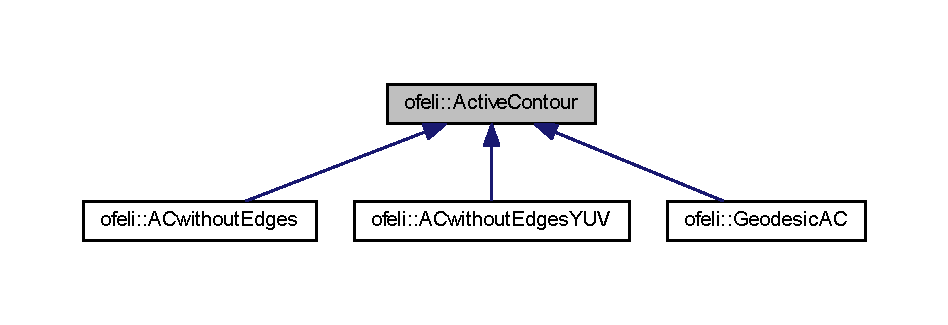
\includegraphics[width=350pt]{classofeli_1_1_active_contour__inherit__graph}
\end{center}
\end{figure}


Collaboration diagram for ofeli\-:\-:Active\-Contour\-:\nopagebreak
\begin{figure}[H]
\begin{center}
\leavevmode
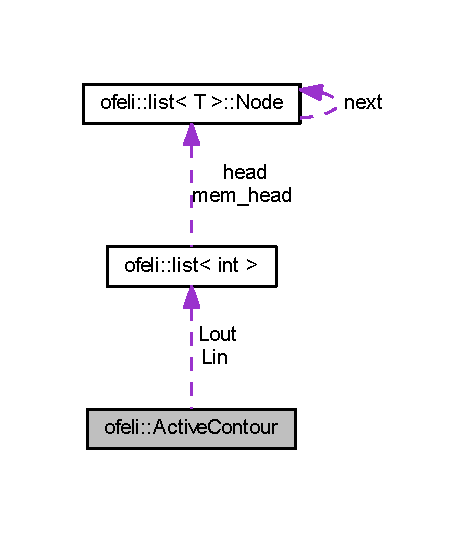
\includegraphics[width=224pt]{classofeli_1_1_active_contour__coll__graph}
\end{center}
\end{figure}
\subsection*{Public Member Functions}
\begin{DoxyCompactItemize}
\item 
\hyperlink{classofeli_1_1_active_contour_abfbc2ecc4b6d511c277eb512ee3749cf}{Active\-Contour} (const unsigned char $\ast$img\-\_\-data1, int img\-\_\-width1, int img\-\_\-height1, bool has\-Ellipse1, double init\-\_\-width1, double init\-\_\-height1, double center\-\_\-x1, double center\-\_\-y1, bool has\-Cycle2\-\_\-1, int kernel\-\_\-length1, double sigma1, int Na1, int Ns1)
\begin{DoxyCompactList}\small\item\em Constructor to initialize the active contour from geometrical parameters of an unique shape, an ellipse or a rectangle. \end{DoxyCompactList}\item 
\hyperlink{classofeli_1_1_active_contour_a38a162e1c928418608067e35c01c1970}{Active\-Contour} (const unsigned char $\ast$img\-\_\-data1, int img\-\_\-width1, int img\-\_\-height1, const char $\ast$phi\-\_\-init1, bool has\-Cycle2\-\_\-1, int kernel\-\_\-length1, double sigma1, int Na1, int Ns1)
\begin{DoxyCompactList}\small\item\em Constructor to initialize the active contour from an initial phi level-\/set function. \end{DoxyCompactList}\item 
\hypertarget{classofeli_1_1_active_contour_a5d077e0b276dea77ea4cdf62ccc50901}{\hyperlink{classofeli_1_1_active_contour_a5d077e0b276dea77ea4cdf62ccc50901}{Active\-Contour} (const \hyperlink{classofeli_1_1_active_contour}{Active\-Contour} \&ac)}\label{classofeli_1_1_active_contour_a5d077e0b276dea77ea4cdf62ccc50901}

\begin{DoxyCompactList}\small\item\em Copy constructor. \end{DoxyCompactList}\item 
\hypertarget{classofeli_1_1_active_contour_af1af6dc1037dda5738dc9964a9476b84}{virtual \hyperlink{classofeli_1_1_active_contour_af1af6dc1037dda5738dc9964a9476b84}{$\sim$\-Active\-Contour} ()}\label{classofeli_1_1_active_contour_af1af6dc1037dda5738dc9964a9476b84}

\begin{DoxyCompactList}\small\item\em Destructor to delete \hyperlink{classofeli_1_1_active_contour_aacb03a6ded4ca51cb52f58aeff955ef7}{phi} and \hyperlink{classofeli_1_1_active_contour_a0f8558877cf436d932838173ba5b8061}{gaussian\-\_\-kernel}. \end{DoxyCompactList}\item 
\hypertarget{classofeli_1_1_active_contour_ac1d127818cc396568532a662951f6f8e}{virtual void \hyperlink{classofeli_1_1_active_contour_ac1d127818cc396568532a662951f6f8e}{initialize\-\_\-for\-\_\-each\-\_\-frame} ()}\label{classofeli_1_1_active_contour_ac1d127818cc396568532a662951f6f8e}

\begin{DoxyCompactList}\small\item\em Initialization for each new frame buffer, used for video tracking. \end{DoxyCompactList}\item 
\hypertarget{classofeli_1_1_active_contour_abf6a4ff642511a4bb2437e11c0943b7e}{void \hyperlink{classofeli_1_1_active_contour_abf6a4ff642511a4bb2437e11c0943b7e}{initialize\-\_\-for\-\_\-each\-\_\-frame} (const unsigned char $\ast$img\-\_\-data1)}\label{classofeli_1_1_active_contour_abf6a4ff642511a4bb2437e11c0943b7e}

\begin{DoxyCompactList}\small\item\em Initialization for each new frame buffer, used for video tracking. \end{DoxyCompactList}\item 
\hypertarget{classofeli_1_1_active_contour_a23013e2eb528bc2fa4e108e928af6f8d}{\hyperlink{classofeli_1_1_active_contour}{Active\-Contour} \& \hyperlink{classofeli_1_1_active_contour_a23013e2eb528bc2fa4e108e928af6f8d}{operator++} ()}\label{classofeli_1_1_active_contour_a23013e2eb528bc2fa4e108e928af6f8d}

\begin{DoxyCompactList}\small\item\em Evolves the active contour of one iteration or one step. This function calls the functions \hyperlink{classofeli_1_1_active_contour_a2ab521c583572158549d416ccc755f3a}{do\-\_\-one\-\_\-iteration\-\_\-in\-\_\-cycle1} or \hyperlink{classofeli_1_1_active_contour_a7cf8243140d8ef8f72a638e9a1442dc2}{do\-\_\-one\-\_\-iteration\-\_\-in\-\_\-cycle2}. \end{DoxyCompactList}\item 
\hypertarget{classofeli_1_1_active_contour_a02cd4d93b90fee487e07f625f337aab1}{void \hyperlink{classofeli_1_1_active_contour_a02cd4d93b90fee487e07f625f337aab1}{evolve} ()}\label{classofeli_1_1_active_contour_a02cd4d93b90fee487e07f625f337aab1}

\begin{DoxyCompactList}\small\item\em Evolves directly the active contour at the final state, i.\-e. it evolves while \hyperlink{classofeli_1_1_active_contour_a610cd07a1013f1b50a5ec5a78c847a40}{is\-Stopped} is not {\ttfamily true}. \end{DoxyCompactList}\item 
\hypertarget{classofeli_1_1_active_contour_a0b5bbfea1f284dd6b94a3ca7883b1373}{void \hyperlink{classofeli_1_1_active_contour_a0b5bbfea1f284dd6b94a3ca7883b1373}{display} () const }\label{classofeli_1_1_active_contour_a0b5bbfea1f284dd6b94a3ca7883b1373}

\begin{DoxyCompactList}\small\item\em Displays the active contour position. \end{DoxyCompactList}\item 
\hypertarget{classofeli_1_1_active_contour_a7b823a8fea40e28c6f27b99158145011}{const char $\ast$ \hyperlink{classofeli_1_1_active_contour_a7b823a8fea40e28c6f27b99158145011}{get\-\_\-phi} () const }\label{classofeli_1_1_active_contour_a7b823a8fea40e28c6f27b99158145011}

\begin{DoxyCompactList}\small\item\em Getter function for the pointer \hyperlink{classofeli_1_1_active_contour_aacb03a6ded4ca51cb52f58aeff955ef7}{phi}. \end{DoxyCompactList}\item 
\hypertarget{classofeli_1_1_active_contour_abfff3ce9cfabd50c3ffc30b93e87b27e}{const \hyperlink{classofeli_1_1list}{ofeli\-::list}$<$ int $>$ \& \hyperlink{classofeli_1_1_active_contour_abfff3ce9cfabd50c3ffc30b93e87b27e}{get\-\_\-\-Lout} () const }\label{classofeli_1_1_active_contour_abfff3ce9cfabd50c3ffc30b93e87b27e}

\begin{DoxyCompactList}\small\item\em Getter function for the linked list \hyperlink{classofeli_1_1_active_contour_a31e0eb18a7ea6ae90acf66ed018fcd85}{Lout}. \end{DoxyCompactList}\item 
\hypertarget{classofeli_1_1_active_contour_af2a8c0c10143490eb7bd3b9c6f14c88d}{const \hyperlink{classofeli_1_1list}{ofeli\-::list}$<$ int $>$ \& \hyperlink{classofeli_1_1_active_contour_af2a8c0c10143490eb7bd3b9c6f14c88d}{get\-\_\-\-Lin} () const }\label{classofeli_1_1_active_contour_af2a8c0c10143490eb7bd3b9c6f14c88d}

\begin{DoxyCompactList}\small\item\em Getter function for the linked list \hyperlink{classofeli_1_1_active_contour_a7662d4f5c8b87d3e642b08b7e341bd79}{Lin}. \end{DoxyCompactList}\item 
\hypertarget{classofeli_1_1_active_contour_abdecbca7ff1f73b2b7ba52d19dfd56f3}{bool \hyperlink{classofeli_1_1_active_contour_abdecbca7ff1f73b2b7ba52d19dfd56f3}{get\-\_\-has\-Lists\-Changes} () const }\label{classofeli_1_1_active_contour_abdecbca7ff1f73b2b7ba52d19dfd56f3}

\begin{DoxyCompactList}\small\item\em Getter function for the boolean \hyperlink{classofeli_1_1_active_contour_acaaac3e08e34cf03c1320c220b188b78}{has\-Lists\-Changes}. \end{DoxyCompactList}\item 
\hypertarget{classofeli_1_1_active_contour_a26b50306becb71e376fc9093f5732e7a}{bool \hyperlink{classofeli_1_1_active_contour_a26b50306becb71e376fc9093f5732e7a}{get\-\_\-has\-Oscillation} () const }\label{classofeli_1_1_active_contour_a26b50306becb71e376fc9093f5732e7a}

\begin{DoxyCompactList}\small\item\em Getter function for the boolean \hyperlink{classofeli_1_1_active_contour_a23e817e4d98cdc2ba8da0b44c5d0ffb8}{has\-Oscillation}. \end{DoxyCompactList}\item 
\hypertarget{classofeli_1_1_active_contour_a7047af04f107b5bb5f18fc719854e1a9}{int \hyperlink{classofeli_1_1_active_contour_a7047af04f107b5bb5f18fc719854e1a9}{get\-\_\-iteration} () const }\label{classofeli_1_1_active_contour_a7047af04f107b5bb5f18fc719854e1a9}

\begin{DoxyCompactList}\small\item\em Getter function for \hyperlink{classofeli_1_1_active_contour_a8723eee8bd5a69dc7c8d7120c642a393}{iteration}. \end{DoxyCompactList}\item 
\hypertarget{classofeli_1_1_active_contour_a88e664f29a5678878b802c886e4d009e}{int \hyperlink{classofeli_1_1_active_contour_a88e664f29a5678878b802c886e4d009e}{get\-\_\-iteration\-\_\-max} () const }\label{classofeli_1_1_active_contour_a88e664f29a5678878b802c886e4d009e}

\begin{DoxyCompactList}\small\item\em Getter function for \hyperlink{classofeli_1_1_active_contour_a7fd09d653e483695eefea4f0e3225bcf}{iteration\-\_\-max}. \end{DoxyCompactList}\item 
\hypertarget{classofeli_1_1_active_contour_a639b05d0dec77fd38b3ace4e4688add3}{bool \hyperlink{classofeli_1_1_active_contour_a639b05d0dec77fd38b3ace4e4688add3}{get\-\_\-is\-Stopped} () const }\label{classofeli_1_1_active_contour_a639b05d0dec77fd38b3ace4e4688add3}

\begin{DoxyCompactList}\small\item\em Getter function for the boolean \hyperlink{classofeli_1_1_active_contour_a610cd07a1013f1b50a5ec5a78c847a40}{is\-Stopped}. \end{DoxyCompactList}\end{DoxyCompactItemize}
\subsection*{Protected Member Functions}
\begin{DoxyCompactItemize}
\item 
\hypertarget{classofeli_1_1_active_contour_a39f22c1bc9d6740180a62520c3f67498}{void \hyperlink{classofeli_1_1_active_contour_a39f22c1bc9d6740180a62520c3f67498}{initialize\-\_\-phi\-\_\-with\-\_\-a\-\_\-shape} (bool has\-Ellipse, double init\-\_\-width, double init\-\_\-height, double center\-\_\-x, double center\-\_\-y)}\label{classofeli_1_1_active_contour_a39f22c1bc9d6740180a62520c3f67498}

\begin{DoxyCompactList}\small\item\em Initialization of \hyperlink{classofeli_1_1_active_contour_aacb03a6ded4ca51cb52f58aeff955ef7}{phi} with a shape. \end{DoxyCompactList}\item 
\hypertarget{classofeli_1_1_active_contour_a181d717496a28d8aac1095d0fc227220}{void \hyperlink{classofeli_1_1_active_contour_a181d717496a28d8aac1095d0fc227220}{initialize\-\_\-lists} ()}\label{classofeli_1_1_active_contour_a181d717496a28d8aac1095d0fc227220}

\begin{DoxyCompactList}\small\item\em Initialization of \hyperlink{classofeli_1_1_active_contour_a31e0eb18a7ea6ae90acf66ed018fcd85}{Lout} and \hyperlink{classofeli_1_1_active_contour_a7662d4f5c8b87d3e642b08b7e341bd79}{Lin}. \end{DoxyCompactList}\item 
\hypertarget{classofeli_1_1_active_contour_ae58a17c4d023abdd142ae24bf8335370}{int \hyperlink{classofeli_1_1_active_contour_ae58a17c4d023abdd142ae24bf8335370}{find\-\_\-offset} (int x, int y) const }\label{classofeli_1_1_active_contour_ae58a17c4d023abdd142ae24bf8335370}

\begin{DoxyCompactList}\small\item\em Calculates the offset of \hyperlink{classofeli_1_1_active_contour_aacb03a6ded4ca51cb52f58aeff955ef7}{phi} or the image data buffer with the position ({\itshape x},{\itshape y}). \end{DoxyCompactList}\item 
\hypertarget{classofeli_1_1_active_contour_adcb560ea7c8b763c7e4e769321807925}{void \hyperlink{classofeli_1_1_active_contour_adcb560ea7c8b763c7e4e769321807925}{find\-\_\-xy\-\_\-position} (int offset, int \&x, int \&y) const }\label{classofeli_1_1_active_contour_adcb560ea7c8b763c7e4e769321807925}

\begin{DoxyCompactList}\small\item\em Calculates the position ({\itshape x},{\itshape y}) of a point of \hyperlink{classofeli_1_1_active_contour_aacb03a6ded4ca51cb52f58aeff955ef7}{phi} or the image with the offset. \end{DoxyCompactList}\end{DoxyCompactItemize}
\subsection*{Static Protected Member Functions}
\begin{DoxyCompactItemize}
\item 
\hypertarget{classofeli_1_1_active_contour_a8a880bf04c5ed62915987145ff05e502}{{\footnotesize template$<$typename T $>$ }\\static T \hyperlink{classofeli_1_1_active_contour_a8a880bf04c5ed62915987145ff05e502}{square} (const T \&value)}\label{classofeli_1_1_active_contour_a8a880bf04c5ed62915987145ff05e502}

\begin{DoxyCompactList}\small\item\em Gives the square of a value. \end{DoxyCompactList}\end{DoxyCompactItemize}
\subsection*{Protected Attributes}
\begin{DoxyCompactItemize}
\item 
\hypertarget{classofeli_1_1_active_contour_a96480d79e9a60817925903da233a5b1e}{const unsigned char $\ast$ \hyperlink{classofeli_1_1_active_contour_a96480d79e9a60817925903da233a5b1e}{img\-\_\-data}}\label{classofeli_1_1_active_contour_a96480d79e9a60817925903da233a5b1e}

\begin{DoxyCompactList}\small\item\em Input pointer on the image data buffer. This buffer must be row-\/wise, except if you define the macro C\-O\-L\-U\-M\-N\-\_\-\-W\-I\-S\-E\-\_\-\-I\-M\-A\-G\-E\-\_\-\-D\-A\-T\-A\-\_\-\-B\-U\-F\-F\-E\-R. \end{DoxyCompactList}\item 
\hypertarget{classofeli_1_1_active_contour_a3623de7ebc0d27ba7fac21a5929afbc6}{const int \hyperlink{classofeli_1_1_active_contour_a3623de7ebc0d27ba7fac21a5929afbc6}{img\-\_\-width}}\label{classofeli_1_1_active_contour_a3623de7ebc0d27ba7fac21a5929afbc6}

\begin{DoxyCompactList}\small\item\em Image width, i.\-e. number of columns. \end{DoxyCompactList}\item 
\hypertarget{classofeli_1_1_active_contour_a88d02b47bab737ec97fe3a7ea9554c0c}{const int \hyperlink{classofeli_1_1_active_contour_a88d02b47bab737ec97fe3a7ea9554c0c}{img\-\_\-height}}\label{classofeli_1_1_active_contour_a88d02b47bab737ec97fe3a7ea9554c0c}

\begin{DoxyCompactList}\small\item\em Image height, i.\-e. number of rows. \end{DoxyCompactList}\item 
\hypertarget{classofeli_1_1_active_contour_a9182e11132f64d7607fbd19a78f58387}{const int \hyperlink{classofeli_1_1_active_contour_a9182e11132f64d7607fbd19a78f58387}{img\-\_\-size}}\label{classofeli_1_1_active_contour_a9182e11132f64d7607fbd19a78f58387}

\begin{DoxyCompactList}\small\item\em Image size, i.\-e. number of pixels. Obviously, it egals to \hyperlink{classofeli_1_1_active_contour_a3623de7ebc0d27ba7fac21a5929afbc6}{img\-\_\-width} × \hyperlink{classofeli_1_1_active_contour_a88d02b47bab737ec97fe3a7ea9554c0c}{img\-\_\-height}. \end{DoxyCompactList}\item 
\hypertarget{classofeli_1_1_active_contour_aacb03a6ded4ca51cb52f58aeff955ef7}{char $\ast$const \hyperlink{classofeli_1_1_active_contour_aacb03a6ded4ca51cb52f58aeff955ef7}{phi}}\label{classofeli_1_1_active_contour_aacb03a6ded4ca51cb52f58aeff955ef7}

\begin{DoxyCompactList}\small\item\em Pointer on the level-\/set function buffer. \end{DoxyCompactList}\end{DoxyCompactItemize}
\subsection*{Private Member Functions}
\begin{DoxyCompactItemize}
\item 
\hypertarget{classofeli_1_1_active_contour_a2ab521c583572158549d416ccc755f3a}{void \hyperlink{classofeli_1_1_active_contour_a2ab521c583572158549d416ccc755f3a}{do\-\_\-one\-\_\-iteration\-\_\-in\-\_\-cycle1} ()}\label{classofeli_1_1_active_contour_a2ab521c583572158549d416ccc755f3a}

\begin{DoxyCompactList}\small\item\em Function called by evolve\-\_\-one\-\_\-iteration() for external or data dependant evolution with {\itshape Fd} speed. \end{DoxyCompactList}\item 
\hypertarget{classofeli_1_1_active_contour_a7cf8243140d8ef8f72a638e9a1442dc2}{void \hyperlink{classofeli_1_1_active_contour_a7cf8243140d8ef8f72a638e9a1442dc2}{do\-\_\-one\-\_\-iteration\-\_\-in\-\_\-cycle2} ()}\label{classofeli_1_1_active_contour_a7cf8243140d8ef8f72a638e9a1442dc2}

\begin{DoxyCompactList}\small\item\em Function called by evolve\-\_\-one\-\_\-iteration() for a curve smoothing or internal evolution with {\itshape Fint} speed. \end{DoxyCompactList}\item 
\hyperlink{classofeli_1_1list}{ofeli\-::list}$<$ int $>$\-::iterator \hyperlink{classofeli_1_1_active_contour_a7d9a557b580af708155ff4ab8bbfd73b}{switch\-\_\-in} (\hyperlink{classofeli_1_1list}{ofeli\-::list}$<$ int $>$\-::iterator Lout\-\_\-point)
\begin{DoxyCompactList}\small\item\em Outward local movement of the curve for a current point ({\itshape x},{\itshape y}) of \hyperlink{classofeli_1_1_active_contour_a31e0eb18a7ea6ae90acf66ed018fcd85}{Lout} that is switched in \hyperlink{classofeli_1_1_active_contour_a7662d4f5c8b87d3e642b08b7e341bd79}{Lin}. \end{DoxyCompactList}\item 
\hypertarget{classofeli_1_1_active_contour_a956318f175100333c4b98aba9253d54a}{void \hyperlink{classofeli_1_1_active_contour_a956318f175100333c4b98aba9253d54a}{add\-\_\-\-Rout\-\_\-neighbor\-\_\-to\-\_\-\-Lout} (int neighbor\-\_\-offset)}\label{classofeli_1_1_active_contour_a956318f175100333c4b98aba9253d54a}

\begin{DoxyCompactList}\small\item\em Second step of procedure \hyperlink{classofeli_1_1_active_contour_a7d9a557b580af708155ff4ab8bbfd73b}{switch\-\_\-in}. \end{DoxyCompactList}\item 
\hyperlink{classofeli_1_1list}{ofeli\-::list}$<$ int $>$\-::iterator \hyperlink{classofeli_1_1_active_contour_a98af656dfc038e6f03c9e4bb67e39bd0}{switch\-\_\-out} (\hyperlink{classofeli_1_1list}{ofeli\-::list}$<$ int $>$\-::iterator Lin\-\_\-point)
\begin{DoxyCompactList}\small\item\em Inward local movement of the curve for a current point ({\itshape x},{\itshape y}) of \hyperlink{classofeli_1_1_active_contour_a7662d4f5c8b87d3e642b08b7e341bd79}{Lin} that is switched in \hyperlink{classofeli_1_1_active_contour_a31e0eb18a7ea6ae90acf66ed018fcd85}{Lout}. \end{DoxyCompactList}\item 
\hypertarget{classofeli_1_1_active_contour_a4c5a0d11f457bc694fb801a153bcd065}{void \hyperlink{classofeli_1_1_active_contour_a4c5a0d11f457bc694fb801a153bcd065}{add\-\_\-\-Rin\-\_\-neighbor\-\_\-to\-\_\-\-Lin} (int neighbor\-\_\-offset)}\label{classofeli_1_1_active_contour_a4c5a0d11f457bc694fb801a153bcd065}

\begin{DoxyCompactList}\small\item\em Second step of procedure \hyperlink{classofeli_1_1_active_contour_a98af656dfc038e6f03c9e4bb67e39bd0}{switch\-\_\-out}. \end{DoxyCompactList}\item 
int \hyperlink{classofeli_1_1_active_contour_ad920bced735a1a78b0bf32e9f452dccb}{compute\-\_\-internal\-\_\-speed\-\_\-\-Fint} (int offset)
\begin{DoxyCompactList}\small\item\em Computes the internal speed Fint for a current point ({\itshape x},{\itshape y}) of \hyperlink{classofeli_1_1_active_contour_a31e0eb18a7ea6ae90acf66ed018fcd85}{Lout} or \hyperlink{classofeli_1_1_active_contour_a7662d4f5c8b87d3e642b08b7e341bd79}{Lin}. \end{DoxyCompactList}\item 
virtual int \hyperlink{classofeli_1_1_active_contour_ae3871b40f2f3e27ae0d75775798cdee1}{compute\-\_\-external\-\_\-speed\-\_\-\-Fd} (int offset)
\begin{DoxyCompactList}\small\item\em Computes the external speed {\itshape Fd} for a current point ({\itshape x},{\itshape y}) of \hyperlink{classofeli_1_1_active_contour_a31e0eb18a7ea6ae90acf66ed018fcd85}{Lout} or \hyperlink{classofeli_1_1_active_contour_a7662d4f5c8b87d3e642b08b7e341bd79}{Lin}. \end{DoxyCompactList}\item 
bool \hyperlink{classofeli_1_1_active_contour_ac734c690a9d10f37b99b6803af335d1d}{is\-Redundant\-Lin\-Point} (int offset) const 
\begin{DoxyCompactList}\small\item\em Finds if a current point ({\itshape x},{\itshape y}) of \hyperlink{classofeli_1_1_active_contour_a7662d4f5c8b87d3e642b08b7e341bd79}{Lin} is redundant. \end{DoxyCompactList}\item 
\hypertarget{classofeli_1_1_active_contour_a1769065c078585aeab98477d0f944b44}{void \hyperlink{classofeli_1_1_active_contour_a1769065c078585aeab98477d0f944b44}{clean\-\_\-\-Lin} ()}\label{classofeli_1_1_active_contour_a1769065c078585aeab98477d0f944b44}

\begin{DoxyCompactList}\small\item\em Eliminates redundant points in \hyperlink{classofeli_1_1_active_contour_a7662d4f5c8b87d3e642b08b7e341bd79}{Lin}. Each point of a list must be connected at least by one point of the other list. \end{DoxyCompactList}\item 
bool \hyperlink{classofeli_1_1_active_contour_a9af52a939f0fd059680383b9d087d6fd}{is\-Redundant\-Lout\-Point} (int offset) const 
\begin{DoxyCompactList}\small\item\em Finds if a current point ({\itshape x},{\itshape y}) of \hyperlink{classofeli_1_1_active_contour_a31e0eb18a7ea6ae90acf66ed018fcd85}{Lout} is redundant. \end{DoxyCompactList}\item 
\hypertarget{classofeli_1_1_active_contour_a17cb6f47e07108bff19a8c45b45c01d1}{void \hyperlink{classofeli_1_1_active_contour_a17cb6f47e07108bff19a8c45b45c01d1}{clean\-\_\-\-Lout} ()}\label{classofeli_1_1_active_contour_a17cb6f47e07108bff19a8c45b45c01d1}

\begin{DoxyCompactList}\small\item\em Eliminates redundant points in \hyperlink{classofeli_1_1_active_contour_a31e0eb18a7ea6ae90acf66ed018fcd85}{Lout}. Each point of a list must be connected at least by one point of the other list. \end{DoxyCompactList}\item 
\hypertarget{classofeli_1_1_active_contour_a403ca7b2a7ed233c9b9cec622140ba60}{virtual void \hyperlink{classofeli_1_1_active_contour_a403ca7b2a7ed233c9b9cec622140ba60}{calculate\-\_\-means} ()}\label{classofeli_1_1_active_contour_a403ca7b2a7ed233c9b9cec622140ba60}

\begin{DoxyCompactList}\small\item\em Specific step reimplemented in the children active contours \hyperlink{classofeli_1_1_a_cwithout_edges}{A\-Cwithout\-Edges} and \hyperlink{classofeli_1_1_a_cwithout_edges_y_u_v}{A\-Cwithout\-Edges\-Y\-U\-V} to calculate the means {\itshape Cout} and {\itshape Cin} in {\itshape O(1)} or {\itshape O}(\hyperlink{classofeli_1_1_active_contour_aefe0738d8a43f3981d591a0cc78ed717}{lists\-\_\-length}) with updates counting and not in {\itshape O}(\hyperlink{classofeli_1_1_active_contour_a9182e11132f64d7607fbd19a78f58387}{img\-\_\-size}). \end{DoxyCompactList}\item 
\hypertarget{classofeli_1_1_active_contour_a72746b8ce52b9cf4ca3549ad6b8ef96b}{virtual void \hyperlink{classofeli_1_1_active_contour_a72746b8ce52b9cf4ca3549ad6b8ef96b}{updates\-\_\-for\-\_\-means\-\_\-in1} ()}\label{classofeli_1_1_active_contour_a72746b8ce52b9cf4ca3549ad6b8ef96b}

\begin{DoxyCompactList}\small\item\em Specific step reimplemented in the children active contours \hyperlink{classofeli_1_1_a_cwithout_edges}{A\-Cwithout\-Edges} and \hyperlink{classofeli_1_1_a_cwithout_edges_y_u_v}{A\-Cwithout\-Edges\-Y\-U\-V} to update the variables to calculate the means {\itshape Cout} and {\itshape Cin} before each \hyperlink{classofeli_1_1_active_contour_a7d9a557b580af708155ff4ab8bbfd73b}{switch\-\_\-in}, in the cycle 1. \end{DoxyCompactList}\item 
virtual void \hyperlink{classofeli_1_1_active_contour_a77e9dc7bcbd0ba48499a499891e021cb}{updates\-\_\-for\-\_\-means\-\_\-in2} (int offset)
\begin{DoxyCompactList}\small\item\em Specific step reimplemented in the children active contours \hyperlink{classofeli_1_1_a_cwithout_edges}{A\-Cwithout\-Edges} and \hyperlink{classofeli_1_1_a_cwithout_edges_y_u_v}{A\-Cwithout\-Edges\-Y\-U\-V} to update the variables to calculate the means {\itshape Cout} and {\itshape Cin} before each \hyperlink{classofeli_1_1_active_contour_a7d9a557b580af708155ff4ab8bbfd73b}{switch\-\_\-in}, in the cycle 2. \end{DoxyCompactList}\item 
\hypertarget{classofeli_1_1_active_contour_aa9bc993165ef307dd52eea763eece326}{virtual void \hyperlink{classofeli_1_1_active_contour_aa9bc993165ef307dd52eea763eece326}{updates\-\_\-for\-\_\-means\-\_\-out1} ()}\label{classofeli_1_1_active_contour_aa9bc993165ef307dd52eea763eece326}

\begin{DoxyCompactList}\small\item\em Specific step reimplemented in the children active contours \hyperlink{classofeli_1_1_a_cwithout_edges}{A\-Cwithout\-Edges} and \hyperlink{classofeli_1_1_a_cwithout_edges_y_u_v}{A\-Cwithout\-Edges\-Y\-U\-V} to update the variables to calculate the means {\itshape Cout} and {\itshape Cin} before each \hyperlink{classofeli_1_1_active_contour_a98af656dfc038e6f03c9e4bb67e39bd0}{switch\-\_\-out}, in the cycle 1. \end{DoxyCompactList}\item 
virtual void \hyperlink{classofeli_1_1_active_contour_a347e650493750ad29b8b73ed52bdcf7a}{updates\-\_\-for\-\_\-means\-\_\-out2} (int offset)
\begin{DoxyCompactList}\small\item\em Specific step reimplemented in the children active contours \hyperlink{classofeli_1_1_a_cwithout_edges}{A\-Cwithout\-Edges} and \hyperlink{classofeli_1_1_a_cwithout_edges_y_u_v}{A\-Cwithout\-Edges\-Y\-U\-V} to update the variables to calculate the means {\itshape Cout} and {\itshape Cin} before each \hyperlink{classofeli_1_1_active_contour_a98af656dfc038e6f03c9e4bb67e39bd0}{switch\-\_\-out}, in the cycle 2. \end{DoxyCompactList}\item 
\hypertarget{classofeli_1_1_active_contour_a7c7275006d98705cd7f04f8a7fe7e697}{void \hyperlink{classofeli_1_1_active_contour_a7c7275006d98705cd7f04f8a7fe7e697}{calculate\-\_\-stopping\-\_\-conditions1} ()}\label{classofeli_1_1_active_contour_a7c7275006d98705cd7f04f8a7fe7e697}

\begin{DoxyCompactList}\small\item\em First stopping condition called at the end of each iteration of the cycle 1. The boolean \hyperlink{classofeli_1_1_active_contour_a0da1bffb7f554ec0b87daa7a0f274d7e}{has\-Last\-Cycle2} is calculated. \end{DoxyCompactList}\item 
\hypertarget{classofeli_1_1_active_contour_a218109b08dd520c95ee7613235bb0593}{void \hyperlink{classofeli_1_1_active_contour_a218109b08dd520c95ee7613235bb0593}{calculate\-\_\-stopping\-\_\-conditions2} ()}\label{classofeli_1_1_active_contour_a218109b08dd520c95ee7613235bb0593}

\begin{DoxyCompactList}\small\item\em Second stopping condition called at the end of the cycle 2. The boolean \hyperlink{classofeli_1_1_active_contour_a610cd07a1013f1b50a5ec5a78c847a40}{is\-Stopped} is calculated. \end{DoxyCompactList}\end{DoxyCompactItemize}
\subsection*{Static Private Member Functions}
\begin{DoxyCompactItemize}
\item 
\hypertarget{classofeli_1_1_active_contour_a6c5e80a286279409a40f279f5e9f848c}{static const int $\ast$const \hyperlink{classofeli_1_1_active_contour_a6c5e80a286279409a40f279f5e9f848c}{make\-\_\-gaussian\-\_\-kernel} (int kernel\-\_\-length1, double sigma1)}\label{classofeli_1_1_active_contour_a6c5e80a286279409a40f279f5e9f848c}

\begin{DoxyCompactList}\small\item\em Creates a normalised gaussian kernel without to divide by {\itshape π} \end{DoxyCompactList}\item 
\hypertarget{classofeli_1_1_active_contour_a419ffe857716df7f33844d93db3d9ace}{static int \hyperlink{classofeli_1_1_active_contour_a419ffe857716df7f33844d93db3d9ace}{signum\-\_\-function} (char value)}\label{classofeli_1_1_active_contour_a419ffe857716df7f33844d93db3d9ace}

\begin{DoxyCompactList}\small\item\em Gives the sign of a value. Return the integer -\/1 or 1. \end{DoxyCompactList}\end{DoxyCompactItemize}
\subsection*{Private Attributes}
\begin{DoxyCompactItemize}
\item 
\hypertarget{classofeli_1_1_active_contour_aa763ff1bed211faa444013cbd5de0be3}{const bool \hyperlink{classofeli_1_1_active_contour_aa763ff1bed211faa444013cbd5de0be3}{has\-Cycle2}}\label{classofeli_1_1_active_contour_aa763ff1bed211faa444013cbd5de0be3}

\begin{DoxyCompactList}\small\item\em Boolean egals to {\ttfamily true} to have the curve smoothing, evolutions in the cycle 2 with the internal speed Fint. \end{DoxyCompactList}\item 
\hypertarget{classofeli_1_1_active_contour_a2b32161d0a9ac64a4e4f4c242fabe27c}{const int \hyperlink{classofeli_1_1_active_contour_a2b32161d0a9ac64a4e4f4c242fabe27c}{kernel\-\_\-length}}\label{classofeli_1_1_active_contour_a2b32161d0a9ac64a4e4f4c242fabe27c}

\begin{DoxyCompactList}\small\item\em Kernel length of the gaussian filter for the curve smoothing. \end{DoxyCompactList}\item 
\hypertarget{classofeli_1_1_active_contour_a66303b7f6b88270133462feb303b039a}{const double \hyperlink{classofeli_1_1_active_contour_a66303b7f6b88270133462feb303b039a}{sigma}}\label{classofeli_1_1_active_contour_a66303b7f6b88270133462feb303b039a}

\begin{DoxyCompactList}\small\item\em Standard deviation of the gaussian kernel for the curve smoothing. \end{DoxyCompactList}\item 
\hypertarget{classofeli_1_1_active_contour_a0f8558877cf436d932838173ba5b8061}{const int $\ast$const \hyperlink{classofeli_1_1_active_contour_a0f8558877cf436d932838173ba5b8061}{gaussian\-\_\-kernel}}\label{classofeli_1_1_active_contour_a0f8558877cf436d932838173ba5b8061}

\begin{DoxyCompactList}\small\item\em Pointer on the gaussian kernel buffer used to calculate Fint. \end{DoxyCompactList}\item 
\hypertarget{classofeli_1_1_active_contour_a8723eee8bd5a69dc7c8d7120c642a393}{int \hyperlink{classofeli_1_1_active_contour_a8723eee8bd5a69dc7c8d7120c642a393}{iteration}}\label{classofeli_1_1_active_contour_a8723eee8bd5a69dc7c8d7120c642a393}

\begin{DoxyCompactList}\small\item\em Number of times the active contour has evolved. \end{DoxyCompactList}\item 
\hypertarget{classofeli_1_1_active_contour_a7fd09d653e483695eefea4f0e3225bcf}{const int \hyperlink{classofeli_1_1_active_contour_a7fd09d653e483695eefea4f0e3225bcf}{iteration\-\_\-max}}\label{classofeli_1_1_active_contour_a7fd09d653e483695eefea4f0e3225bcf}

\begin{DoxyCompactList}\small\item\em Maximum number of times the active contour can evolve. \end{DoxyCompactList}\item 
\hypertarget{classofeli_1_1_active_contour_a610cd07a1013f1b50a5ec5a78c847a40}{bool \hyperlink{classofeli_1_1_active_contour_a610cd07a1013f1b50a5ec5a78c847a40}{is\-Stopped}}\label{classofeli_1_1_active_contour_a610cd07a1013f1b50a5ec5a78c847a40}

\begin{DoxyCompactList}\small\item\em Boolean egals to {\ttfamily true} to stop the algorithm. \end{DoxyCompactList}\item 
\hypertarget{classofeli_1_1_active_contour_a31e0eb18a7ea6ae90acf66ed018fcd85}{\hyperlink{classofeli_1_1list}{ofeli\-::list}$<$ int $>$ \hyperlink{classofeli_1_1_active_contour_a31e0eb18a7ea6ae90acf66ed018fcd85}{Lout}}\label{classofeli_1_1_active_contour_a31e0eb18a7ea6ae90acf66ed018fcd85}

\begin{DoxyCompactList}\small\item\em List of points belong to the outside boundary. \end{DoxyCompactList}\item 
\hypertarget{classofeli_1_1_active_contour_a7662d4f5c8b87d3e642b08b7e341bd79}{\hyperlink{classofeli_1_1list}{ofeli\-::list}$<$ int $>$ \hyperlink{classofeli_1_1_active_contour_a7662d4f5c8b87d3e642b08b7e341bd79}{Lin}}\label{classofeli_1_1_active_contour_a7662d4f5c8b87d3e642b08b7e341bd79}

\begin{DoxyCompactList}\small\item\em List of points belong to the inside boundary. \end{DoxyCompactList}\item 
\hypertarget{classofeli_1_1_active_contour_a00740d5331e8d4f60c1345cc8cabf7ad}{const int \hyperlink{classofeli_1_1_active_contour_a00740d5331e8d4f60c1345cc8cabf7ad}{kernel\-\_\-radius}}\label{classofeli_1_1_active_contour_a00740d5331e8d4f60c1345cc8cabf7ad}

\begin{DoxyCompactList}\small\item\em {\itshape kernel\-\_\-radius} = ( \hyperlink{classofeli_1_1_active_contour_a2b32161d0a9ac64a4e4f4c242fabe27c}{kernel\-\_\-length} -\/ 1) / 2 with \hyperlink{classofeli_1_1_active_contour_a2b32161d0a9ac64a4e4f4c242fabe27c}{kernel\-\_\-length} impair. \end{DoxyCompactList}\item 
\hypertarget{classofeli_1_1_active_contour_a9dcea2f4d6803007fe98e38152adf000}{bool \hyperlink{classofeli_1_1_active_contour_a9dcea2f4d6803007fe98e38152adf000}{has\-Outward\-Evolution}}\label{classofeli_1_1_active_contour_a9dcea2f4d6803007fe98e38152adf000}

\begin{DoxyCompactList}\small\item\em Boolean egals to {\ttfamily true} if one point of \hyperlink{classofeli_1_1_active_contour_a31e0eb18a7ea6ae90acf66ed018fcd85}{Lout} at least is switched in during the scan through the \hyperlink{classofeli_1_1_active_contour_a31e0eb18a7ea6ae90acf66ed018fcd85}{Lout} list. \end{DoxyCompactList}\item 
\hypertarget{classofeli_1_1_active_contour_af437460aa2cdf312166a3fe4d54beeb4}{bool \hyperlink{classofeli_1_1_active_contour_af437460aa2cdf312166a3fe4d54beeb4}{has\-Inward\-Evolution}}\label{classofeli_1_1_active_contour_af437460aa2cdf312166a3fe4d54beeb4}

\begin{DoxyCompactList}\small\item\em Boolean egals to {\ttfamily true} if one point of \hyperlink{classofeli_1_1_active_contour_a7662d4f5c8b87d3e642b08b7e341bd79}{Lin} at least is switched out during the scan through the \hyperlink{classofeli_1_1_active_contour_a7662d4f5c8b87d3e642b08b7e341bd79}{Lin} list. \end{DoxyCompactList}\item 
\hypertarget{classofeli_1_1_active_contour_a59f111cd0910d2e6534b51bb1da3c254}{int \hyperlink{classofeli_1_1_active_contour_a59f111cd0910d2e6534b51bb1da3c254}{Na}}\label{classofeli_1_1_active_contour_a59f111cd0910d2e6534b51bb1da3c254}

\begin{DoxyCompactList}\small\item\em Number of iterations the active contour evolves in the cycle 1 with {\itshape Fd} speed. \end{DoxyCompactList}\item 
\hypertarget{classofeli_1_1_active_contour_a811a28ec9c39400d244783a8a2fe7e2d}{const int \hyperlink{classofeli_1_1_active_contour_a811a28ec9c39400d244783a8a2fe7e2d}{Na\-\_\-max}}\label{classofeli_1_1_active_contour_a811a28ec9c39400d244783a8a2fe7e2d}

\begin{DoxyCompactList}\small\item\em Number of maximum iterations the active contour evolves in the cycle 1 with {\itshape Fd} speed. \end{DoxyCompactList}\item 
\hypertarget{classofeli_1_1_active_contour_a38cc27ae9706801882322f02b5db2df8}{int \hyperlink{classofeli_1_1_active_contour_a38cc27ae9706801882322f02b5db2df8}{Ns}}\label{classofeli_1_1_active_contour_a38cc27ae9706801882322f02b5db2df8}

\begin{DoxyCompactList}\small\item\em Number of iterations the active contour evolves in the cycle 2 with {\itshape Fint} speed. \end{DoxyCompactList}\item 
\hypertarget{classofeli_1_1_active_contour_a908322f93a50ce7808960236478649fe}{const int \hyperlink{classofeli_1_1_active_contour_a908322f93a50ce7808960236478649fe}{Ns\-\_\-max}}\label{classofeli_1_1_active_contour_a908322f93a50ce7808960236478649fe}

\begin{DoxyCompactList}\small\item\em Number of maximum iterations the active contour evolves in the cycle 2 with {\itshape Fint} speed. \end{DoxyCompactList}\item 
\hypertarget{classofeli_1_1_active_contour_acaaac3e08e34cf03c1320c220b188b78}{bool \hyperlink{classofeli_1_1_active_contour_acaaac3e08e34cf03c1320c220b188b78}{has\-Lists\-Changes}}\label{classofeli_1_1_active_contour_acaaac3e08e34cf03c1320c220b188b78}

\begin{DoxyCompactList}\small\item\em Boolean egals to true if \hyperlink{classofeli_1_1_active_contour_a9dcea2f4d6803007fe98e38152adf000}{has\-Outward\-Evolution} egals to {\ttfamily true} or \hyperlink{classofeli_1_1_active_contour_af437460aa2cdf312166a3fe4d54beeb4}{has\-Inward\-Evolution} egals to {\ttfamily true}. \end{DoxyCompactList}\item 
\hypertarget{classofeli_1_1_active_contour_aefe0738d8a43f3981d591a0cc78ed717}{int \hyperlink{classofeli_1_1_active_contour_aefe0738d8a43f3981d591a0cc78ed717}{lists\-\_\-length}}\label{classofeli_1_1_active_contour_aefe0738d8a43f3981d591a0cc78ed717}

\begin{DoxyCompactList}\small\item\em Length of \hyperlink{classofeli_1_1_active_contour_a7662d4f5c8b87d3e642b08b7e341bd79}{Lin} + length of \hyperlink{classofeli_1_1_active_contour_a31e0eb18a7ea6ae90acf66ed018fcd85}{Lout}. \end{DoxyCompactList}\item 
\hypertarget{classofeli_1_1_active_contour_a653c2bcd37ed61e9eacda89a013590d4}{int \hyperlink{classofeli_1_1_active_contour_a653c2bcd37ed61e9eacda89a013590d4}{previous\-\_\-lists\-\_\-length}}\label{classofeli_1_1_active_contour_a653c2bcd37ed61e9eacda89a013590d4}

\begin{DoxyCompactList}\small\item\em Length of \hyperlink{classofeli_1_1_active_contour_a7662d4f5c8b87d3e642b08b7e341bd79}{Lin} + length of \hyperlink{classofeli_1_1_active_contour_a31e0eb18a7ea6ae90acf66ed018fcd85}{Lout} of the previous iteration. \end{DoxyCompactList}\item 
\hypertarget{classofeli_1_1_active_contour_a23e817e4d98cdc2ba8da0b44c5d0ffb8}{bool \hyperlink{classofeli_1_1_active_contour_a23e817e4d98cdc2ba8da0b44c5d0ffb8}{has\-Oscillation}}\label{classofeli_1_1_active_contour_a23e817e4d98cdc2ba8da0b44c5d0ffb8}

\begin{DoxyCompactList}\small\item\em Boolean calculated at the end of the cycle 2 with function {\itshape \hyperlink{classofeli_1_1_active_contour_a218109b08dd520c95ee7613235bb0593}{calculate\-\_\-stopping\-\_\-conditions2()}}. \end{DoxyCompactList}\item 
\hypertarget{classofeli_1_1_active_contour_a01b0cfb6e5593b267bceb72e288cfe88}{int \hyperlink{classofeli_1_1_active_contour_a01b0cfb6e5593b267bceb72e288cfe88}{oscillations\-\_\-in\-\_\-a\-\_\-row}}\label{classofeli_1_1_active_contour_a01b0cfb6e5593b267bceb72e288cfe88}

\begin{DoxyCompactList}\small\item\em To count the number of times the relative gap of the lists length are less of a constant, fixed at 1\%, i.\-e. the number of consecutive oscillations. \end{DoxyCompactList}\item 
\hypertarget{classofeli_1_1_active_contour_a0da1bffb7f554ec0b87daa7a0f274d7e}{bool \hyperlink{classofeli_1_1_active_contour_a0da1bffb7f554ec0b87daa7a0f274d7e}{has\-Last\-Cycle2}}\label{classofeli_1_1_active_contour_a0da1bffb7f554ec0b87daa7a0f274d7e}

\begin{DoxyCompactList}\small\item\em Boolean calculated at the end of each iteration of the cycle 1 with function {\itshape \hyperlink{classofeli_1_1_active_contour_a7c7275006d98705cd7f04f8a7fe7e697}{calculate\-\_\-stopping\-\_\-conditions1()}}. \end{DoxyCompactList}\end{DoxyCompactItemize}
\subsection*{Friends}
\begin{DoxyCompactItemize}
\item 
\hypertarget{classofeli_1_1_active_contour_a4ae6d808948cb0fe309be0d4c4d39755}{std\-::ostream \& \hyperlink{classofeli_1_1_active_contour_a4ae6d808948cb0fe309be0d4c4d39755}{operator$<$$<$} (std\-::ostream \&os, const \hyperlink{classofeli_1_1_active_contour}{Active\-Contour} \&ac)}\label{classofeli_1_1_active_contour_a4ae6d808948cb0fe309be0d4c4d39755}

\begin{DoxyCompactList}\small\item\em Overloading of cout $<$$<$. It displays the active contour position. \end{DoxyCompactList}\end{DoxyCompactItemize}


\subsection{Detailed Description}
The class \hyperlink{classofeli_1_1_active_contour}{Active\-Contour} contains the implementation of the Fast-\/\-Two-\/\-Cycle (F\-T\-C) algorithm of Shi and Karl as it describes in their article \char`\"{}\-A real-\/time algorithm for the approximation of level-\/set based curve evolution\char`\"{} published in I\-E\-E\-E Transactions on Image Processing in may 2008. This class should be never instantiated because the function to calculate the external speed {\itshape Fd} is too general. The 3 classes \hyperlink{classofeli_1_1_a_cwithout_edges}{ofeli\-::\-A\-Cwithout\-Edges}, \hyperlink{classofeli_1_1_a_cwithout_edges_y_u_v}{ofeli\-::\-A\-Cwithout\-Edges\-Y\-U\-V} and \hyperlink{classofeli_1_1_geodesic_a_c}{ofeli\-::\-Geodesic\-A\-C}, inherit of the class \hyperlink{classofeli_1_1_active_contour}{Active\-Contour}, with for each class it own implementation of this function. 

Definition at line 49 of file activecontour.\-hpp.



\subsection{Constructor \& Destructor Documentation}
\hypertarget{classofeli_1_1_active_contour_abfbc2ecc4b6d511c277eb512ee3749cf}{\index{ofeli\-::\-Active\-Contour@{ofeli\-::\-Active\-Contour}!Active\-Contour@{Active\-Contour}}
\index{Active\-Contour@{Active\-Contour}!ofeli::ActiveContour@{ofeli\-::\-Active\-Contour}}
\subsubsection[{Active\-Contour}]{\setlength{\rightskip}{0pt plus 5cm}Active\-Contour\-::\-Active\-Contour (
\begin{DoxyParamCaption}
\item[{const unsigned char $\ast$}]{img\-\_\-data1, }
\item[{int}]{img\-\_\-width1, }
\item[{int}]{img\-\_\-height1, }
\item[{bool}]{has\-Ellipse1, }
\item[{double}]{init\-\_\-width1, }
\item[{double}]{init\-\_\-height1, }
\item[{double}]{center\-\_\-x1, }
\item[{double}]{center\-\_\-y1, }
\item[{bool}]{has\-Cycle2\-\_\-1, }
\item[{int}]{kernel\-\_\-length1, }
\item[{double}]{sigma1, }
\item[{int}]{Na1, }
\item[{int}]{Ns1}
\end{DoxyParamCaption}
)}}\label{classofeli_1_1_active_contour_abfbc2ecc4b6d511c277eb512ee3749cf}


Constructor to initialize the active contour from geometrical parameters of an unique shape, an ellipse or a rectangle. 


\begin{DoxyParams}{Parameters}
{\em img\-\_\-data1} & Input pointer on the image data buffer. This buffer must be row-\/wise, except if you define the macro C\-O\-L\-U\-M\-N\-\_\-\-W\-I\-S\-E\-\_\-\-I\-M\-A\-G\-E\-\_\-\-D\-A\-T\-A\-\_\-\-B\-U\-F\-F\-E\-R. Passed to \hyperlink{classofeli_1_1_active_contour_a96480d79e9a60817925903da233a5b1e}{img\-\_\-data}. \\
\hline
{\em img\-\_\-width1} & Image width, i.\-e. number of columns. Passed to \hyperlink{classofeli_1_1_active_contour_a3623de7ebc0d27ba7fac21a5929afbc6}{img\-\_\-width}. \\
\hline
{\em img\-\_\-height1} & Image height, i.\-e. number of rows. Passed to \hyperlink{classofeli_1_1_active_contour_a88d02b47bab737ec97fe3a7ea9554c0c}{img\-\_\-height}. \\
\hline
{\em has\-Ellipse1} & Boolean to choose the shape of the active contour initialization, {\ttfamily true} for an ellipse or {\ttfamily false} for a rectangle. \\
\hline
{\em init\-\_\-width1} & Width of the shape divided by the image \hyperlink{classofeli_1_1_active_contour_a3623de7ebc0d27ba7fac21a5929afbc6}{img\-\_\-width}. \\
\hline
{\em init\-\_\-height1} & Height of the shape divided by the image \hyperlink{classofeli_1_1_active_contour_a88d02b47bab737ec97fe3a7ea9554c0c}{img\-\_\-height}. \\
\hline
{\em center\-\_\-x1} & X-\/axis position or column index of the center of the shape divided by the image \hyperlink{classofeli_1_1_active_contour_a3623de7ebc0d27ba7fac21a5929afbc6}{img\-\_\-width} subtracted by 0.\-5. \\
\hline
{\em center\-\_\-y1} & Y-\/axis position or row index of the center of the shape divided by the image \hyperlink{classofeli_1_1_active_contour_a88d02b47bab737ec97fe3a7ea9554c0c}{img\-\_\-height} subtracted by 0.\-5.\par
 To have the center of the shape into the image \-: -\/0.\-5 $<$ center\-\_\-x1 $<$ 0.\-5 and -\/0.\-5 $<$ center\-\_\-y1 $<$ 0.\-5. \\
\hline
{\em has\-Cycle2\-\_\-1} & Boolean to have or not the curve smoothing, evolutions in the cycle 2 with an internal speed Fint. Passed to \hyperlink{classofeli_1_1_active_contour_aa763ff1bed211faa444013cbd5de0be3}{has\-Cycle2}. \\
\hline
{\em kernel\-\_\-length1} & Kernel length of the gaussian filter for the curve smoothing. Passed to \hyperlink{classofeli_1_1_active_contour_a2b32161d0a9ac64a4e4f4c242fabe27c}{kernel\-\_\-length}. \\
\hline
{\em sigma1} & Standard deviation of the gaussian kernel for the curve smoothing. Passed to \hyperlink{classofeli_1_1_active_contour_a66303b7f6b88270133462feb303b039a}{sigma}. \\
\hline
{\em Na1} & Number of maximum iterations the active contour evolves in the cycle 1, external or data dependant evolutions with {\itshape Fd} speed. Passed to \hyperlink{classofeli_1_1_active_contour_a811a28ec9c39400d244783a8a2fe7e2d}{Na\-\_\-max}. \\
\hline
{\em Ns1} & Number of maximum iterations the active contour evolves in the cycle 2, curve smoothing or internal evolutions with {\itshape Fint} speed. Passed to \hyperlink{classofeli_1_1_active_contour_a908322f93a50ce7808960236478649fe}{Ns\-\_\-max}. \\
\hline
\end{DoxyParams}


Definition at line 66 of file activecontour.\-cpp.



Here is the call graph for this function\-:\nopagebreak
\begin{figure}[H]
\begin{center}
\leavevmode
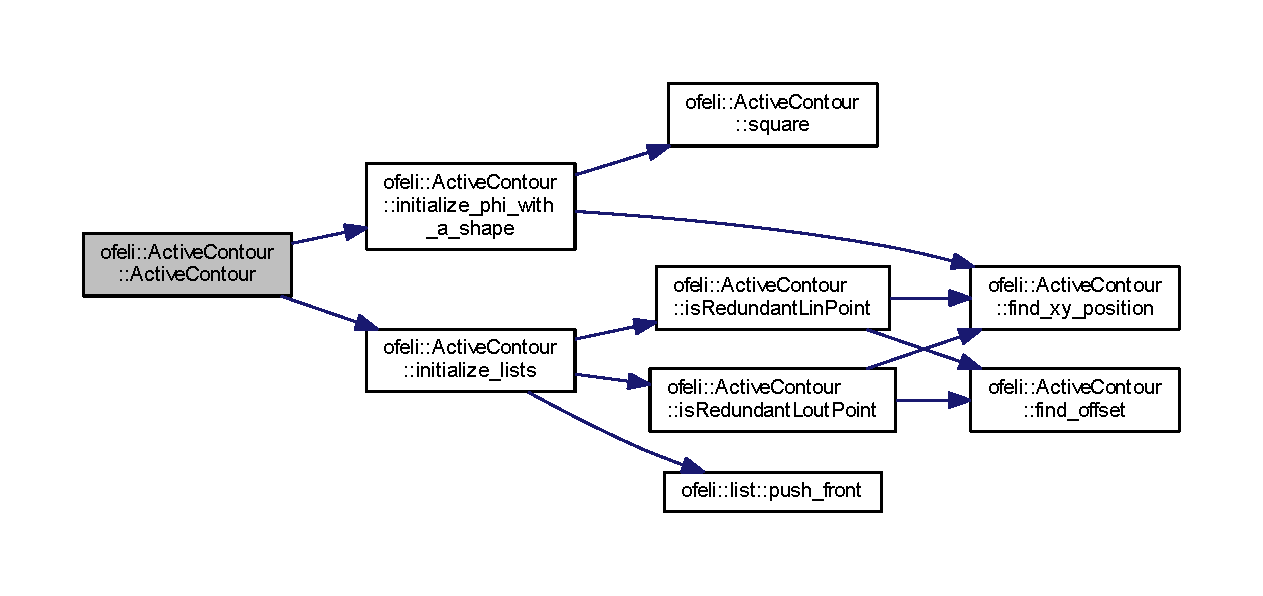
\includegraphics[width=350pt]{classofeli_1_1_active_contour_abfbc2ecc4b6d511c277eb512ee3749cf_cgraph}
\end{center}
\end{figure}


\hypertarget{classofeli_1_1_active_contour_a38a162e1c928418608067e35c01c1970}{\index{ofeli\-::\-Active\-Contour@{ofeli\-::\-Active\-Contour}!Active\-Contour@{Active\-Contour}}
\index{Active\-Contour@{Active\-Contour}!ofeli::ActiveContour@{ofeli\-::\-Active\-Contour}}
\subsubsection[{Active\-Contour}]{\setlength{\rightskip}{0pt plus 5cm}Active\-Contour\-::\-Active\-Contour (
\begin{DoxyParamCaption}
\item[{const unsigned char $\ast$}]{img\-\_\-data1, }
\item[{int}]{img\-\_\-width1, }
\item[{int}]{img\-\_\-height1, }
\item[{const char $\ast$}]{phi\-\_\-init1, }
\item[{bool}]{has\-Cycle2\-\_\-1, }
\item[{int}]{kernel\-\_\-length1, }
\item[{double}]{sigma1, }
\item[{int}]{Na1, }
\item[{int}]{Ns1}
\end{DoxyParamCaption}
)}}\label{classofeli_1_1_active_contour_a38a162e1c928418608067e35c01c1970}


Constructor to initialize the active contour from an initial phi level-\/set function. 


\begin{DoxyParams}{Parameters}
{\em img\-\_\-data1} & Input pointer on the image data buffer. This buffer must be row-\/wise, except if you define the macro C\-O\-L\-U\-M\-N\-\_\-\-W\-I\-S\-E\-\_\-\-I\-M\-A\-G\-E\-\_\-\-D\-A\-T\-A\-\_\-\-B\-U\-F\-F\-E\-R. Passed to \hyperlink{classofeli_1_1_active_contour_a96480d79e9a60817925903da233a5b1e}{img\-\_\-data}. \\
\hline
{\em img\-\_\-width1} & Image width, i.\-e. number of columns. Passed to \hyperlink{classofeli_1_1_active_contour_a3623de7ebc0d27ba7fac21a5929afbc6}{img\-\_\-width}. \\
\hline
{\em img\-\_\-height1} & Image height, i.\-e. number of rows. Passed to \hyperlink{classofeli_1_1_active_contour_a88d02b47bab737ec97fe3a7ea9554c0c}{img\-\_\-height}. \\
\hline
{\em phi\-\_\-init1} & Pointer on the initialized level-\/set function buffer. Copied to \hyperlink{classofeli_1_1_active_contour_aacb03a6ded4ca51cb52f58aeff955ef7}{phi}. \hyperlink{classofeli_1_1_active_contour_aacb03a6ded4ca51cb52f58aeff955ef7}{phi} is checked and cleaned if needed after so {\itshape phi\-\_\-init1} can be a binarized buffer with 1 for outside region and -\/1 for inside region to simplify your task. \\
\hline
{\em has\-Cycle2\-\_\-1} & Boolean to have or not the curve smoothing, evolutions in the cycle 2 with an internal speed Fint. Passed to \hyperlink{classofeli_1_1_active_contour_aa763ff1bed211faa444013cbd5de0be3}{has\-Cycle2}. \\
\hline
{\em kernel\-\_\-length1} & Kernel length of the gaussian filter for the curve smoothing. Passed to \hyperlink{classofeli_1_1_active_contour_a2b32161d0a9ac64a4e4f4c242fabe27c}{kernel\-\_\-length}. \\
\hline
{\em sigma1} & Standard deviation of the gaussian kernel for the curve smoothing. Passed to \hyperlink{classofeli_1_1_active_contour_a66303b7f6b88270133462feb303b039a}{sigma}. \\
\hline
{\em Na1} & Number of maximum iterations the active contour evolves in the cycle 1, external or data dependant evolutions with {\itshape Fd} speed. Passed to \hyperlink{classofeli_1_1_active_contour_a811a28ec9c39400d244783a8a2fe7e2d}{Na\-\_\-max}. \\
\hline
{\em Ns1} & Number of maximum iterations the active contour evolves in the cycle 2, curve smoothing or internal evolutions with {\itshape Fint} speed. Passed to \hyperlink{classofeli_1_1_active_contour_a908322f93a50ce7808960236478649fe}{Ns\-\_\-max}. \\
\hline
\end{DoxyParams}


Definition at line 87 of file activecontour.\-cpp.



Here is the call graph for this function\-:\nopagebreak
\begin{figure}[H]
\begin{center}
\leavevmode
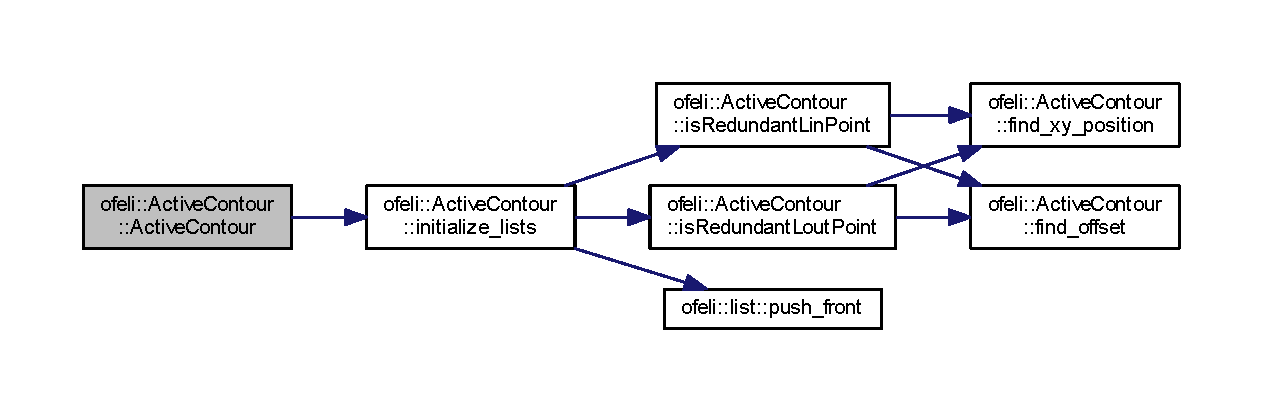
\includegraphics[width=350pt]{classofeli_1_1_active_contour_a38a162e1c928418608067e35c01c1970_cgraph}
\end{center}
\end{figure}




\subsection{Member Function Documentation}
\hypertarget{classofeli_1_1_active_contour_ae3871b40f2f3e27ae0d75775798cdee1}{\index{ofeli\-::\-Active\-Contour@{ofeli\-::\-Active\-Contour}!compute\-\_\-external\-\_\-speed\-\_\-\-Fd@{compute\-\_\-external\-\_\-speed\-\_\-\-Fd}}
\index{compute\-\_\-external\-\_\-speed\-\_\-\-Fd@{compute\-\_\-external\-\_\-speed\-\_\-\-Fd}!ofeli::ActiveContour@{ofeli\-::\-Active\-Contour}}
\subsubsection[{compute\-\_\-external\-\_\-speed\-\_\-\-Fd}]{\setlength{\rightskip}{0pt plus 5cm}int Active\-Contour\-::compute\-\_\-external\-\_\-speed\-\_\-\-Fd (
\begin{DoxyParamCaption}
\item[{int}]{offset}
\end{DoxyParamCaption}
)\hspace{0.3cm}{\ttfamily [private]}, {\ttfamily [virtual]}}}\label{classofeli_1_1_active_contour_ae3871b40f2f3e27ae0d75775798cdee1}


Computes the external speed {\itshape Fd} for a current point ({\itshape x},{\itshape y}) of \hyperlink{classofeli_1_1_active_contour_a31e0eb18a7ea6ae90acf66ed018fcd85}{Lout} or \hyperlink{classofeli_1_1_active_contour_a7662d4f5c8b87d3e642b08b7e341bd79}{Lin}. 


\begin{DoxyParams}{Parameters}
{\em offset} & offset of the image data buffer with {\itshape offset} = {\itshape x} + {\itshape y} × \hyperlink{classofeli_1_1_active_contour_a3623de7ebc0d27ba7fac21a5929afbc6}{img\-\_\-width} \\
\hline
\end{DoxyParams}
\begin{DoxyReturn}{Returns}
Fd, the external speed for the data dependant evolution of the active contour used in the cycle 1 
\end{DoxyReturn}


Reimplemented in \hyperlink{classofeli_1_1_a_cwithout_edges_y_u_v_ae61e98ace069646a009de7cd7148e065}{ofeli\-::\-A\-Cwithout\-Edges\-Y\-U\-V}, \hyperlink{classofeli_1_1_a_cwithout_edges_a4190840f934080ff6eb64fa48c993f98}{ofeli\-::\-A\-Cwithout\-Edges}, and \hyperlink{classofeli_1_1_geodesic_a_c_a1e4d1d3011526eaff49b5404f00f27f9}{ofeli\-::\-Geodesic\-A\-C}.



Definition at line 996 of file activecontour.\-cpp.



Here is the caller graph for this function\-:\nopagebreak
\begin{figure}[H]
\begin{center}
\leavevmode
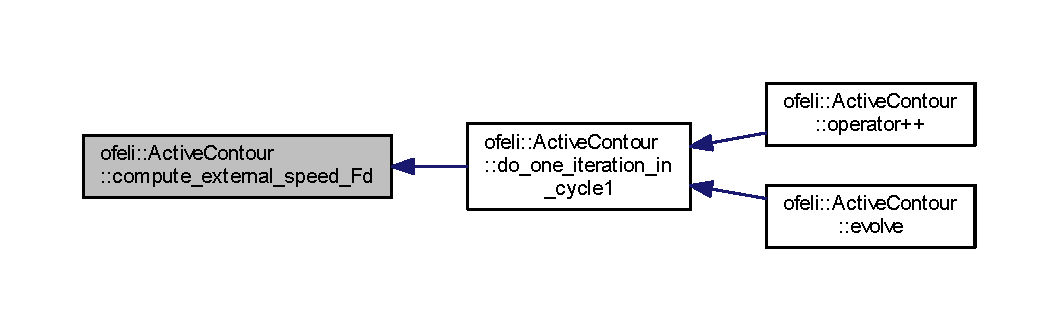
\includegraphics[width=350pt]{classofeli_1_1_active_contour_ae3871b40f2f3e27ae0d75775798cdee1_icgraph}
\end{center}
\end{figure}


\hypertarget{classofeli_1_1_active_contour_ad920bced735a1a78b0bf32e9f452dccb}{\index{ofeli\-::\-Active\-Contour@{ofeli\-::\-Active\-Contour}!compute\-\_\-internal\-\_\-speed\-\_\-\-Fint@{compute\-\_\-internal\-\_\-speed\-\_\-\-Fint}}
\index{compute\-\_\-internal\-\_\-speed\-\_\-\-Fint@{compute\-\_\-internal\-\_\-speed\-\_\-\-Fint}!ofeli::ActiveContour@{ofeli\-::\-Active\-Contour}}
\subsubsection[{compute\-\_\-internal\-\_\-speed\-\_\-\-Fint}]{\setlength{\rightskip}{0pt plus 5cm}int Active\-Contour\-::compute\-\_\-internal\-\_\-speed\-\_\-\-Fint (
\begin{DoxyParamCaption}
\item[{int}]{offset}
\end{DoxyParamCaption}
)\hspace{0.3cm}{\ttfamily [private]}}}\label{classofeli_1_1_active_contour_ad920bced735a1a78b0bf32e9f452dccb}


Computes the internal speed Fint for a current point ({\itshape x},{\itshape y}) of \hyperlink{classofeli_1_1_active_contour_a31e0eb18a7ea6ae90acf66ed018fcd85}{Lout} or \hyperlink{classofeli_1_1_active_contour_a7662d4f5c8b87d3e642b08b7e341bd79}{Lin}. 


\begin{DoxyParams}{Parameters}
{\em offset} & offset of the buffer pointed by \hyperlink{classofeli_1_1_active_contour_aacb03a6ded4ca51cb52f58aeff955ef7}{phi} with {\itshape offset} = {\itshape x} + {\itshape y} × \hyperlink{classofeli_1_1_active_contour_a3623de7ebc0d27ba7fac21a5929afbc6}{img\-\_\-width} \\
\hline
\end{DoxyParams}
\begin{DoxyReturn}{Returns}
Fint, the internal speed for the regularization of the active contour used in the cycle 2 
\end{DoxyReturn}


Definition at line 715 of file activecontour.\-cpp.



Here is the call graph for this function\-:\nopagebreak
\begin{figure}[H]
\begin{center}
\leavevmode
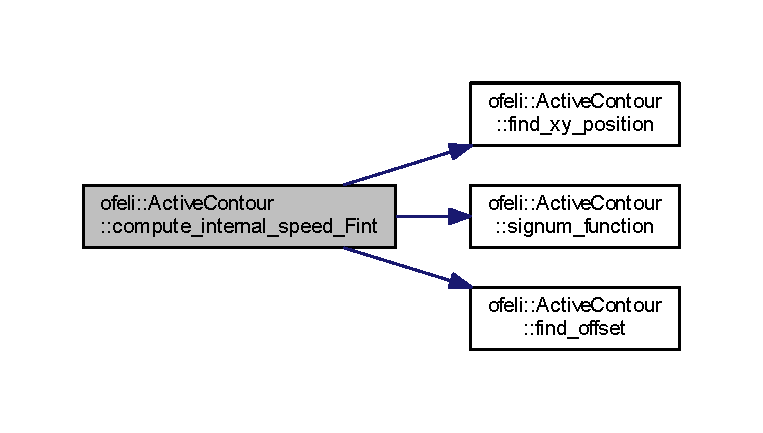
\includegraphics[width=350pt]{classofeli_1_1_active_contour_ad920bced735a1a78b0bf32e9f452dccb_cgraph}
\end{center}
\end{figure}




Here is the caller graph for this function\-:\nopagebreak
\begin{figure}[H]
\begin{center}
\leavevmode
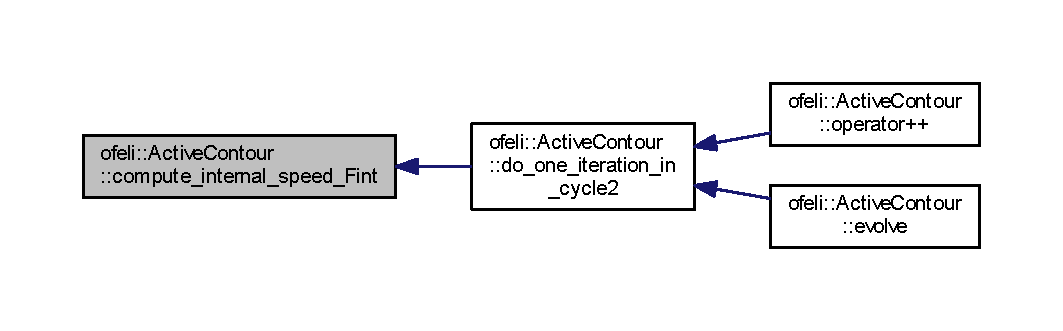
\includegraphics[width=350pt]{classofeli_1_1_active_contour_ad920bced735a1a78b0bf32e9f452dccb_icgraph}
\end{center}
\end{figure}


\hypertarget{classofeli_1_1_active_contour_ac734c690a9d10f37b99b6803af335d1d}{\index{ofeli\-::\-Active\-Contour@{ofeli\-::\-Active\-Contour}!is\-Redundant\-Lin\-Point@{is\-Redundant\-Lin\-Point}}
\index{is\-Redundant\-Lin\-Point@{is\-Redundant\-Lin\-Point}!ofeli::ActiveContour@{ofeli\-::\-Active\-Contour}}
\subsubsection[{is\-Redundant\-Lin\-Point}]{\setlength{\rightskip}{0pt plus 5cm}bool Active\-Contour\-::is\-Redundant\-Lin\-Point (
\begin{DoxyParamCaption}
\item[{int}]{offset}
\end{DoxyParamCaption}
) const\hspace{0.3cm}{\ttfamily [private]}}}\label{classofeli_1_1_active_contour_ac734c690a9d10f37b99b6803af335d1d}


Finds if a current point ({\itshape x},{\itshape y}) of \hyperlink{classofeli_1_1_active_contour_a7662d4f5c8b87d3e642b08b7e341bd79}{Lin} is redundant. 


\begin{DoxyParams}{Parameters}
{\em offset} & offset of the buffer pointed by \hyperlink{classofeli_1_1_active_contour_aacb03a6ded4ca51cb52f58aeff955ef7}{phi} with {\itshape offset} = {\itshape x} + {\itshape y} × \hyperlink{classofeli_1_1_active_contour_a3623de7ebc0d27ba7fac21a5929afbc6}{img\-\_\-width} \\
\hline
\end{DoxyParams}
\begin{DoxyReturn}{Returns}
{\ttfamily true} if the point ({\itshape x},{\itshape y}) of \hyperlink{classofeli_1_1_active_contour_a7662d4f5c8b87d3e642b08b7e341bd79}{Lin} is redundant, otherwise, {\ttfamily false} 
\end{DoxyReturn}


Definition at line 760 of file activecontour.\-cpp.



Here is the call graph for this function\-:\nopagebreak
\begin{figure}[H]
\begin{center}
\leavevmode
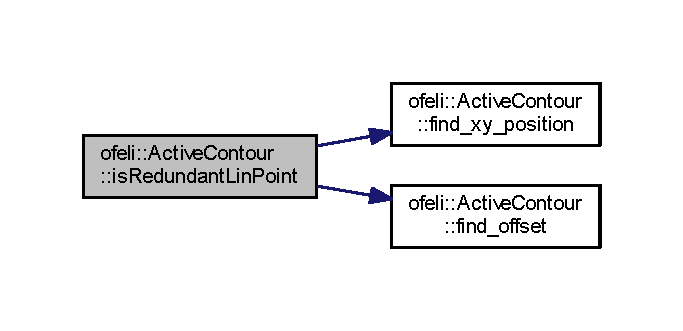
\includegraphics[width=328pt]{classofeli_1_1_active_contour_ac734c690a9d10f37b99b6803af335d1d_cgraph}
\end{center}
\end{figure}




Here is the caller graph for this function\-:\nopagebreak
\begin{figure}[H]
\begin{center}
\leavevmode
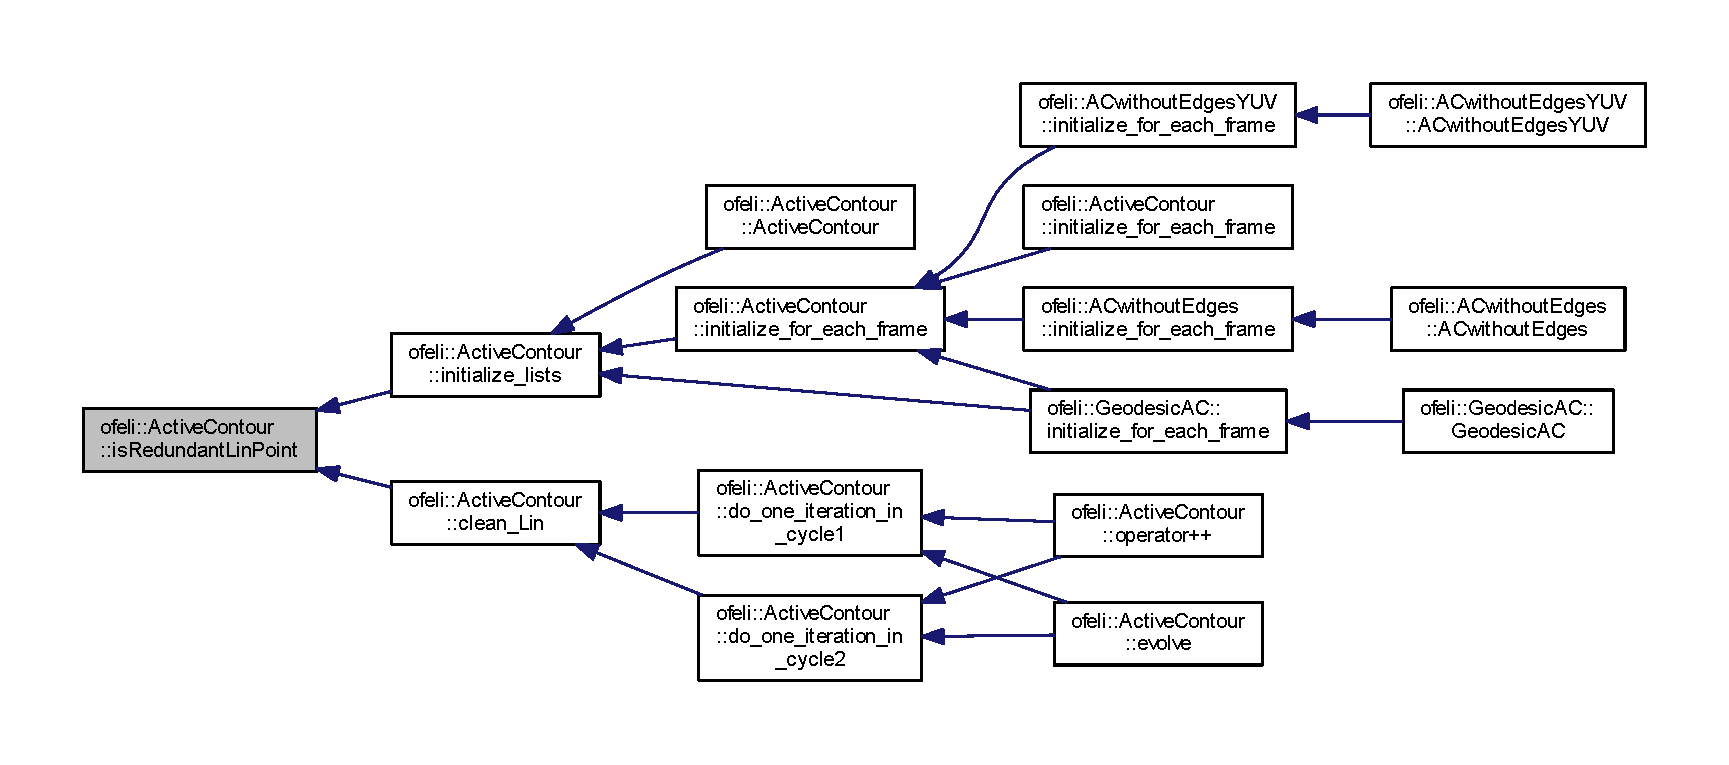
\includegraphics[width=350pt]{classofeli_1_1_active_contour_ac734c690a9d10f37b99b6803af335d1d_icgraph}
\end{center}
\end{figure}


\hypertarget{classofeli_1_1_active_contour_a9af52a939f0fd059680383b9d087d6fd}{\index{ofeli\-::\-Active\-Contour@{ofeli\-::\-Active\-Contour}!is\-Redundant\-Lout\-Point@{is\-Redundant\-Lout\-Point}}
\index{is\-Redundant\-Lout\-Point@{is\-Redundant\-Lout\-Point}!ofeli::ActiveContour@{ofeli\-::\-Active\-Contour}}
\subsubsection[{is\-Redundant\-Lout\-Point}]{\setlength{\rightskip}{0pt plus 5cm}bool Active\-Contour\-::is\-Redundant\-Lout\-Point (
\begin{DoxyParamCaption}
\item[{int}]{offset}
\end{DoxyParamCaption}
) const\hspace{0.3cm}{\ttfamily [private]}}}\label{classofeli_1_1_active_contour_a9af52a939f0fd059680383b9d087d6fd}


Finds if a current point ({\itshape x},{\itshape y}) of \hyperlink{classofeli_1_1_active_contour_a31e0eb18a7ea6ae90acf66ed018fcd85}{Lout} is redundant. 


\begin{DoxyParams}{Parameters}
{\em offset} & offset of the buffer pointed by \hyperlink{classofeli_1_1_active_contour_aacb03a6ded4ca51cb52f58aeff955ef7}{phi} with {\itshape offset} = {\itshape x} + {\itshape y} × \hyperlink{classofeli_1_1_active_contour_a3623de7ebc0d27ba7fac21a5929afbc6}{img\-\_\-width} \\
\hline
\end{DoxyParams}
\begin{DoxyReturn}{Returns}
{\ttfamily true} if the point ({\itshape x},{\itshape y}) of \hyperlink{classofeli_1_1_active_contour_a31e0eb18a7ea6ae90acf66ed018fcd85}{Lout} is redundant, otherwise, {\ttfamily false} 
\end{DoxyReturn}


Definition at line 852 of file activecontour.\-cpp.



Here is the call graph for this function\-:\nopagebreak
\begin{figure}[H]
\begin{center}
\leavevmode
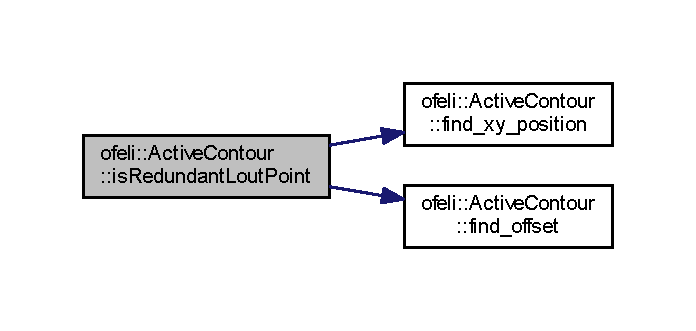
\includegraphics[width=334pt]{classofeli_1_1_active_contour_a9af52a939f0fd059680383b9d087d6fd_cgraph}
\end{center}
\end{figure}




Here is the caller graph for this function\-:\nopagebreak
\begin{figure}[H]
\begin{center}
\leavevmode
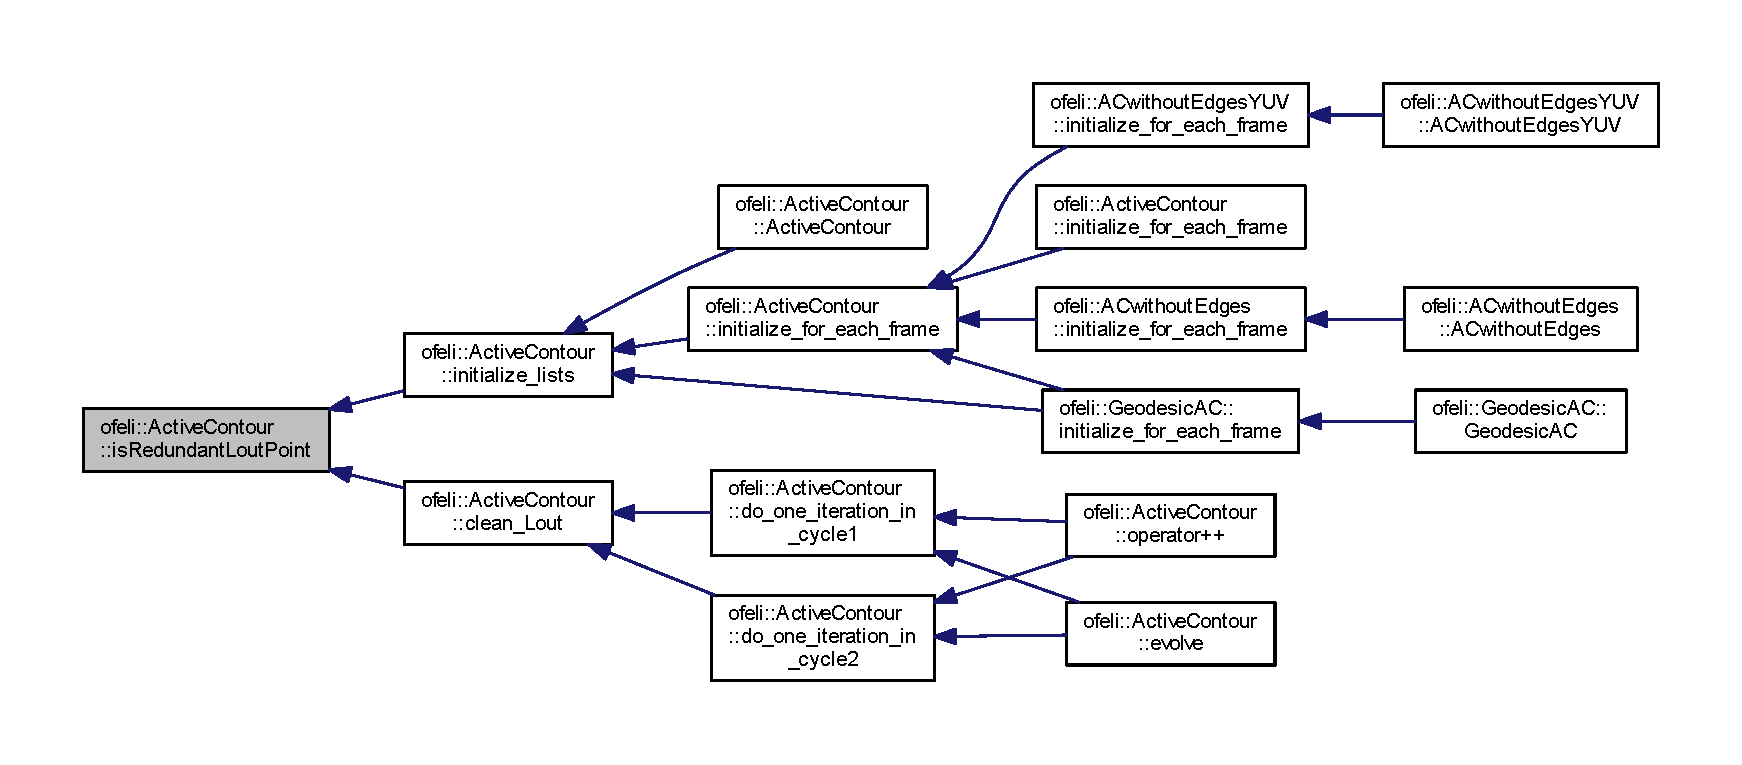
\includegraphics[width=350pt]{classofeli_1_1_active_contour_a9af52a939f0fd059680383b9d087d6fd_icgraph}
\end{center}
\end{figure}


\hypertarget{classofeli_1_1_active_contour_a7d9a557b580af708155ff4ab8bbfd73b}{\index{ofeli\-::\-Active\-Contour@{ofeli\-::\-Active\-Contour}!switch\-\_\-in@{switch\-\_\-in}}
\index{switch\-\_\-in@{switch\-\_\-in}!ofeli::ActiveContour@{ofeli\-::\-Active\-Contour}}
\subsubsection[{switch\-\_\-in}]{\setlength{\rightskip}{0pt plus 5cm}void Active\-Contour\-::switch\-\_\-in (
\begin{DoxyParamCaption}
\item[{{\bf ofeli\-::list}$<$ int $>$\-::iterator}]{Lout\-\_\-point}
\end{DoxyParamCaption}
)\hspace{0.3cm}{\ttfamily [private]}}}\label{classofeli_1_1_active_contour_a7d9a557b580af708155ff4ab8bbfd73b}


Outward local movement of the curve for a current point ({\itshape x},{\itshape y}) of \hyperlink{classofeli_1_1_active_contour_a31e0eb18a7ea6ae90acf66ed018fcd85}{Lout} that is switched in \hyperlink{classofeli_1_1_active_contour_a7662d4f5c8b87d3e642b08b7e341bd79}{Lin}. 


\begin{DoxyParams}{Parameters}
{\em Lout\-\_\-point} & iterator which contains offset of the buffer pointed by \hyperlink{classofeli_1_1_active_contour_aacb03a6ded4ca51cb52f58aeff955ef7}{phi} with {\itshape offset} = {\itshape x} + {\itshape y} × \hyperlink{classofeli_1_1_active_contour_a3623de7ebc0d27ba7fac21a5929afbc6}{img\-\_\-width} \\
\hline
\end{DoxyParams}


Definition at line 563 of file activecontour.\-cpp.



Here is the call graph for this function\-:\nopagebreak
\begin{figure}[H]
\begin{center}
\leavevmode
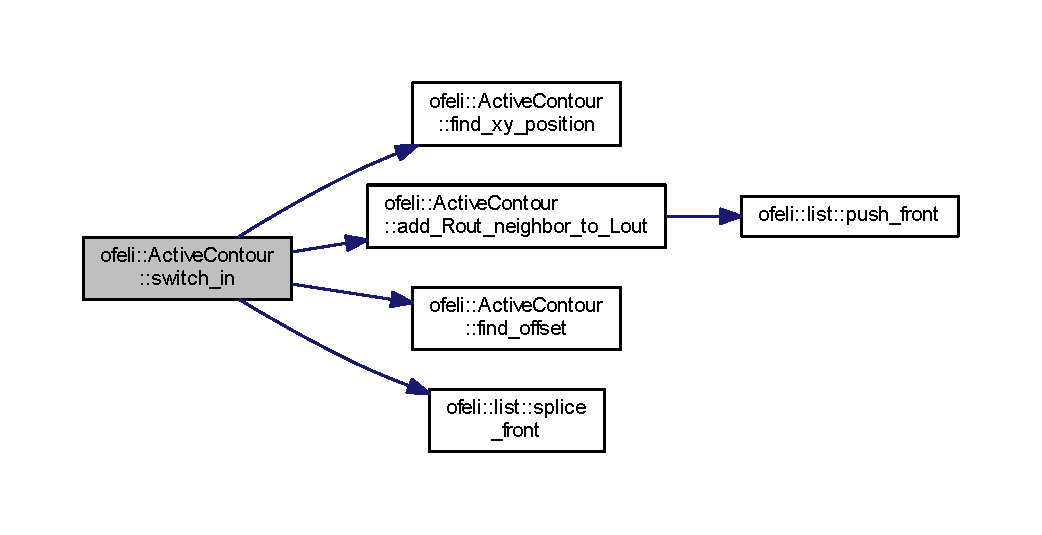
\includegraphics[width=350pt]{classofeli_1_1_active_contour_a7d9a557b580af708155ff4ab8bbfd73b_cgraph}
\end{center}
\end{figure}




Here is the caller graph for this function\-:\nopagebreak
\begin{figure}[H]
\begin{center}
\leavevmode
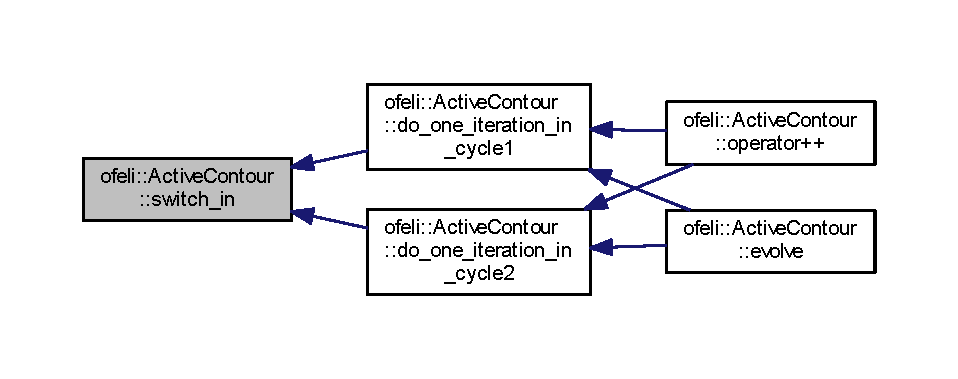
\includegraphics[width=350pt]{classofeli_1_1_active_contour_a7d9a557b580af708155ff4ab8bbfd73b_icgraph}
\end{center}
\end{figure}


\hypertarget{classofeli_1_1_active_contour_a98af656dfc038e6f03c9e4bb67e39bd0}{\index{ofeli\-::\-Active\-Contour@{ofeli\-::\-Active\-Contour}!switch\-\_\-out@{switch\-\_\-out}}
\index{switch\-\_\-out@{switch\-\_\-out}!ofeli::ActiveContour@{ofeli\-::\-Active\-Contour}}
\subsubsection[{switch\-\_\-out}]{\setlength{\rightskip}{0pt plus 5cm}void Active\-Contour\-::switch\-\_\-out (
\begin{DoxyParamCaption}
\item[{{\bf ofeli\-::list}$<$ int $>$\-::iterator}]{Lin\-\_\-point}
\end{DoxyParamCaption}
)\hspace{0.3cm}{\ttfamily [private]}}}\label{classofeli_1_1_active_contour_a98af656dfc038e6f03c9e4bb67e39bd0}


Inward local movement of the curve for a current point ({\itshape x},{\itshape y}) of \hyperlink{classofeli_1_1_active_contour_a7662d4f5c8b87d3e642b08b7e341bd79}{Lin} that is switched in \hyperlink{classofeli_1_1_active_contour_a31e0eb18a7ea6ae90acf66ed018fcd85}{Lout}. 


\begin{DoxyParams}{Parameters}
{\em Lin\-\_\-point} & which contains offset of the buffer pointed by \hyperlink{classofeli_1_1_active_contour_aacb03a6ded4ca51cb52f58aeff955ef7}{phi} with {\itshape offset} = {\itshape x} + {\itshape y} × \hyperlink{classofeli_1_1_active_contour_a3623de7ebc0d27ba7fac21a5929afbc6}{img\-\_\-width} \\
\hline
\end{DoxyParams}


Definition at line 639 of file activecontour.\-cpp.



Here is the call graph for this function\-:\nopagebreak
\begin{figure}[H]
\begin{center}
\leavevmode
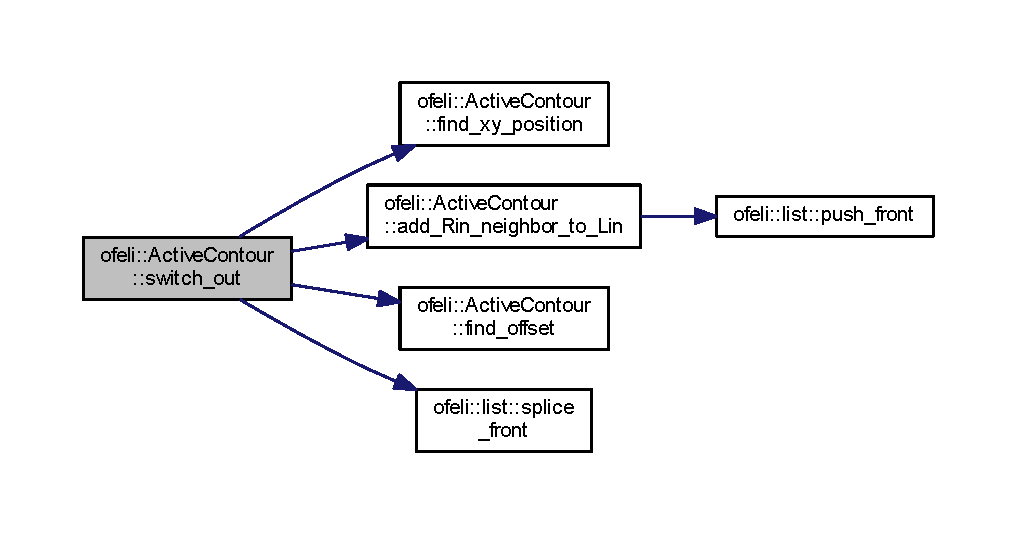
\includegraphics[width=350pt]{classofeli_1_1_active_contour_a98af656dfc038e6f03c9e4bb67e39bd0_cgraph}
\end{center}
\end{figure}




Here is the caller graph for this function\-:\nopagebreak
\begin{figure}[H]
\begin{center}
\leavevmode
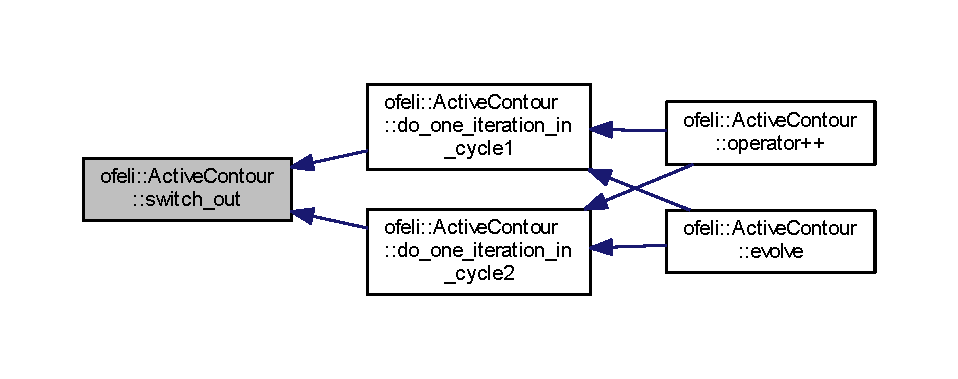
\includegraphics[width=350pt]{classofeli_1_1_active_contour_a98af656dfc038e6f03c9e4bb67e39bd0_icgraph}
\end{center}
\end{figure}


\hypertarget{classofeli_1_1_active_contour_a77e9dc7bcbd0ba48499a499891e021cb}{\index{ofeli\-::\-Active\-Contour@{ofeli\-::\-Active\-Contour}!updates\-\_\-for\-\_\-means\-\_\-in2@{updates\-\_\-for\-\_\-means\-\_\-in2}}
\index{updates\-\_\-for\-\_\-means\-\_\-in2@{updates\-\_\-for\-\_\-means\-\_\-in2}!ofeli::ActiveContour@{ofeli\-::\-Active\-Contour}}
\subsubsection[{updates\-\_\-for\-\_\-means\-\_\-in2}]{\setlength{\rightskip}{0pt plus 5cm}void Active\-Contour\-::updates\-\_\-for\-\_\-means\-\_\-in2 (
\begin{DoxyParamCaption}
\item[{int}]{offset}
\end{DoxyParamCaption}
)\hspace{0.3cm}{\ttfamily [private]}, {\ttfamily [virtual]}}}\label{classofeli_1_1_active_contour_a77e9dc7bcbd0ba48499a499891e021cb}


Specific step reimplemented in the children active contours \hyperlink{classofeli_1_1_a_cwithout_edges}{A\-Cwithout\-Edges} and \hyperlink{classofeli_1_1_a_cwithout_edges_y_u_v}{A\-Cwithout\-Edges\-Y\-U\-V} to update the variables to calculate the means {\itshape Cout} and {\itshape Cin} before each \hyperlink{classofeli_1_1_active_contour_a7d9a557b580af708155ff4ab8bbfd73b}{switch\-\_\-in}, in the cycle 2. 


\begin{DoxyParams}{Parameters}
{\em offset} & offset of the image data buffer with {\itshape offset} = {\itshape x} + {\itshape y} × \hyperlink{classofeli_1_1_active_contour_a3623de7ebc0d27ba7fac21a5929afbc6}{img\-\_\-width} \\
\hline
\end{DoxyParams}


Reimplemented in \hyperlink{classofeli_1_1_a_cwithout_edges_y_u_v_a249aa0e9664cf4f024997ac4475fe70c}{ofeli\-::\-A\-Cwithout\-Edges\-Y\-U\-V}, and \hyperlink{classofeli_1_1_a_cwithout_edges_aae62ec3548eb47ca5f67c2ede19a251b}{ofeli\-::\-A\-Cwithout\-Edges}.



Definition at line 1130 of file activecontour.\-cpp.



Here is the caller graph for this function\-:\nopagebreak
\begin{figure}[H]
\begin{center}
\leavevmode
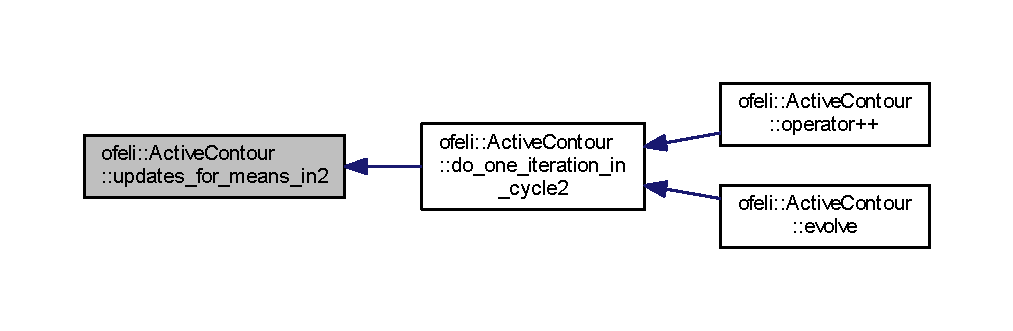
\includegraphics[width=350pt]{classofeli_1_1_active_contour_a77e9dc7bcbd0ba48499a499891e021cb_icgraph}
\end{center}
\end{figure}


\hypertarget{classofeli_1_1_active_contour_a347e650493750ad29b8b73ed52bdcf7a}{\index{ofeli\-::\-Active\-Contour@{ofeli\-::\-Active\-Contour}!updates\-\_\-for\-\_\-means\-\_\-out2@{updates\-\_\-for\-\_\-means\-\_\-out2}}
\index{updates\-\_\-for\-\_\-means\-\_\-out2@{updates\-\_\-for\-\_\-means\-\_\-out2}!ofeli::ActiveContour@{ofeli\-::\-Active\-Contour}}
\subsubsection[{updates\-\_\-for\-\_\-means\-\_\-out2}]{\setlength{\rightskip}{0pt plus 5cm}void Active\-Contour\-::updates\-\_\-for\-\_\-means\-\_\-out2 (
\begin{DoxyParamCaption}
\item[{int}]{offset}
\end{DoxyParamCaption}
)\hspace{0.3cm}{\ttfamily [private]}, {\ttfamily [virtual]}}}\label{classofeli_1_1_active_contour_a347e650493750ad29b8b73ed52bdcf7a}


Specific step reimplemented in the children active contours \hyperlink{classofeli_1_1_a_cwithout_edges}{A\-Cwithout\-Edges} and \hyperlink{classofeli_1_1_a_cwithout_edges_y_u_v}{A\-Cwithout\-Edges\-Y\-U\-V} to update the variables to calculate the means {\itshape Cout} and {\itshape Cin} before each \hyperlink{classofeli_1_1_active_contour_a98af656dfc038e6f03c9e4bb67e39bd0}{switch\-\_\-out}, in the cycle 2. 


\begin{DoxyParams}{Parameters}
{\em offset} & offset of the image data buffer with {\itshape offset} = {\itshape x} + {\itshape y} × \hyperlink{classofeli_1_1_active_contour_a3623de7ebc0d27ba7fac21a5929afbc6}{img\-\_\-width} \\
\hline
\end{DoxyParams}


Reimplemented in \hyperlink{classofeli_1_1_a_cwithout_edges_y_u_v_a43b463f3b8d5cb9604fd73b18083409a}{ofeli\-::\-A\-Cwithout\-Edges\-Y\-U\-V}, and \hyperlink{classofeli_1_1_a_cwithout_edges_a80021d0ca688f3cbf46bccc870706e4c}{ofeli\-::\-A\-Cwithout\-Edges}.



Definition at line 1135 of file activecontour.\-cpp.



Here is the caller graph for this function\-:\nopagebreak
\begin{figure}[H]
\begin{center}
\leavevmode
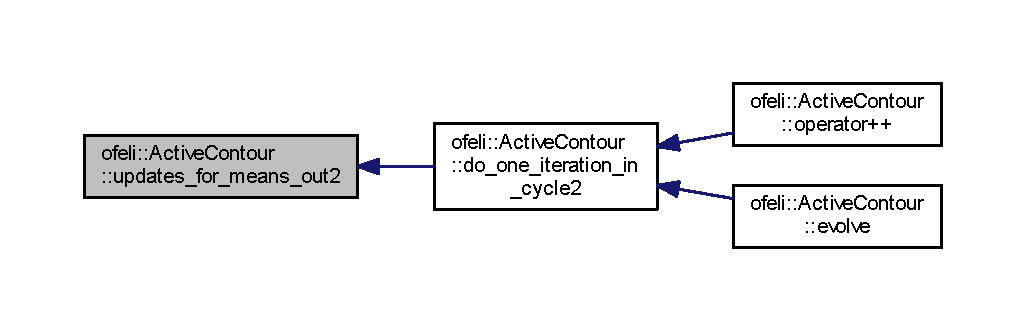
\includegraphics[width=350pt]{classofeli_1_1_active_contour_a347e650493750ad29b8b73ed52bdcf7a_icgraph}
\end{center}
\end{figure}




The documentation for this class was generated from the following files\-:\begin{DoxyCompactItemize}
\item 
activecontour.\-hpp\item 
activecontour.\-cpp\end{DoxyCompactItemize}

\hypertarget{classofeli_1_1_a_cwithout_edges}{\section{ofeli\-:\-:A\-Cwithout\-Edges Class Reference}
\label{classofeli_1_1_a_cwithout_edges}\index{ofeli\-::\-A\-Cwithout\-Edges@{ofeli\-::\-A\-Cwithout\-Edges}}
}


{\ttfamily \#include $<$ac\-\_\-withoutedges.\-hpp$>$}



Inheritance diagram for ofeli\-:\-:A\-Cwithout\-Edges\-:\nopagebreak
\begin{figure}[H]
\begin{center}
\leavevmode
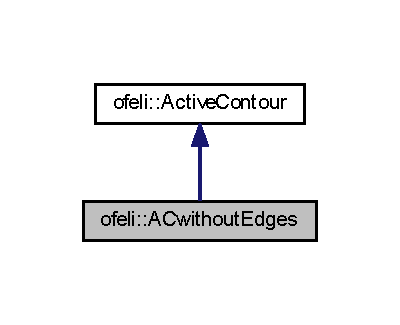
\includegraphics[width=192pt]{classofeli_1_1_a_cwithout_edges__inherit__graph}
\end{center}
\end{figure}


Collaboration diagram for ofeli\-:\-:A\-Cwithout\-Edges\-:\nopagebreak
\begin{figure}[H]
\begin{center}
\leavevmode
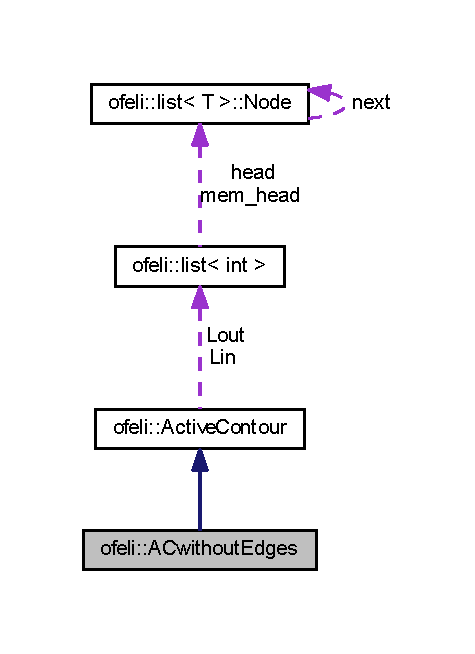
\includegraphics[width=228pt]{classofeli_1_1_a_cwithout_edges__coll__graph}
\end{center}
\end{figure}
\subsection*{Public Member Functions}
\begin{DoxyCompactItemize}
\item 
\hypertarget{classofeli_1_1_a_cwithout_edges_a50545482590fb3d7ea40df3382452dfb}{\hyperlink{classofeli_1_1_a_cwithout_edges_a50545482590fb3d7ea40df3382452dfb}{A\-Cwithout\-Edges} (const unsigned char $\ast$img\-\_\-data1, int img\-\_\-width1, int img\-\_\-height1)}\label{classofeli_1_1_a_cwithout_edges_a50545482590fb3d7ea40df3382452dfb}

\begin{DoxyCompactList}\small\item\em Constructor to initialize the active contour with a centered rectangle and the default values of the algorithm parameters. \end{DoxyCompactList}\item 
\hyperlink{classofeli_1_1_a_cwithout_edges_ad3be07385b0a0d693036ddee99bdaf2b}{A\-Cwithout\-Edges} (const unsigned char $\ast$img\-\_\-data1, int img\-\_\-width1, int img\-\_\-height1, bool has\-Ellipse1, double init\-\_\-width1, double init\-\_\-height1, double center\-\_\-x1, double center\-\_\-y1, bool has\-Cycle2\-\_\-1, int kernel\-\_\-length1, double sigma1, int Na1, int Ns1, int lambda\-\_\-out1, int lambda\-\_\-in1)
\begin{DoxyCompactList}\small\item\em Constructor to initialize the active contour from geometrical parameters of an unique shape, an ellipse or a rectangle. \end{DoxyCompactList}\item 
\hyperlink{classofeli_1_1_a_cwithout_edges_a3aafada5bffe3d4251ff22cd22ebb401}{A\-Cwithout\-Edges} (const unsigned char $\ast$img\-\_\-data1, int img\-\_\-width1, int img\-\_\-height1, const char $\ast$phi\-\_\-init1, bool has\-Cycle2\-\_\-1, int kernel\-\_\-length1, double sigma1, int Na1, int Ns1, int lambda\-\_\-out1, int lambda\-\_\-in1)
\begin{DoxyCompactList}\small\item\em Constructor to initialize the active contour from an initial phi level-\/set function. \end{DoxyCompactList}\item 
\hypertarget{classofeli_1_1_a_cwithout_edges_ad5d3e6800f33e0fdd396adcd031ca401}{\hyperlink{classofeli_1_1_a_cwithout_edges_ad5d3e6800f33e0fdd396adcd031ca401}{A\-Cwithout\-Edges} (const \hyperlink{classofeli_1_1_a_cwithout_edges}{A\-Cwithout\-Edges} \&ac)}\label{classofeli_1_1_a_cwithout_edges_ad5d3e6800f33e0fdd396adcd031ca401}

\begin{DoxyCompactList}\small\item\em Copy constructor. \end{DoxyCompactList}\item 
\hypertarget{classofeli_1_1_a_cwithout_edges_a73ac34cabdc4aae95531996e394d59a7}{virtual void \hyperlink{classofeli_1_1_a_cwithout_edges_a73ac34cabdc4aae95531996e394d59a7}{initialize\-\_\-for\-\_\-each\-\_\-frame} ()}\label{classofeli_1_1_a_cwithout_edges_a73ac34cabdc4aae95531996e394d59a7}

\begin{DoxyCompactList}\small\item\em Initialization for each new frame buffer, used for video tracking. \end{DoxyCompactList}\item 
\hypertarget{classofeli_1_1_a_cwithout_edges_af6248d9b93cf8a651824216b2dd175b9}{int \hyperlink{classofeli_1_1_a_cwithout_edges_af6248d9b93cf8a651824216b2dd175b9}{get\-\_\-\-Cout} () const }\label{classofeli_1_1_a_cwithout_edges_af6248d9b93cf8a651824216b2dd175b9}

\begin{DoxyCompactList}\small\item\em Getter function for \hyperlink{classofeli_1_1_a_cwithout_edges_a02c32b73dcc676251330a42b6fb4e6f4}{Cout}. \end{DoxyCompactList}\item 
\hypertarget{classofeli_1_1_a_cwithout_edges_ad4da88f6edd9e97f16d783182a1bcb3a}{int \hyperlink{classofeli_1_1_a_cwithout_edges_ad4da88f6edd9e97f16d783182a1bcb3a}{get\-\_\-\-Cin} () const }\label{classofeli_1_1_a_cwithout_edges_ad4da88f6edd9e97f16d783182a1bcb3a}

\begin{DoxyCompactList}\small\item\em Getter function for \hyperlink{classofeli_1_1_a_cwithout_edges_af26f696be73588b2a150c3eef6f62c85}{Cin}. \end{DoxyCompactList}\end{DoxyCompactItemize}
\subsection*{Private Member Functions}
\begin{DoxyCompactItemize}
\item 
\hypertarget{classofeli_1_1_a_cwithout_edges_a39c8f6940d7574aadec3953b4704e8af}{void \hyperlink{classofeli_1_1_a_cwithout_edges_a39c8f6940d7574aadec3953b4704e8af}{initialize\-\_\-sums} ()}\label{classofeli_1_1_a_cwithout_edges_a39c8f6940d7574aadec3953b4704e8af}

\begin{DoxyCompactList}\small\item\em Initializes the variables \hyperlink{classofeli_1_1_a_cwithout_edges_a14f61eabccbac71bf616674e8feb44f5}{sum\-\_\-in}, \hyperlink{classofeli_1_1_a_cwithout_edges_a799b4078bc22cbde48cc29c93727efc5}{sum\-\_\-out}, \hyperlink{classofeli_1_1_a_cwithout_edges_a8d2c28710176ae9b562b4001f8171348}{n\-\_\-in} and \hyperlink{classofeli_1_1_a_cwithout_edges_a07818e5c3700b0164037e982077de10c}{n\-\_\-out} with scanning through the image. \end{DoxyCompactList}\item 
\hypertarget{classofeli_1_1_a_cwithout_edges_a6dd4cde332938ec033cb8a5e870ec132}{virtual void \hyperlink{classofeli_1_1_a_cwithout_edges_a6dd4cde332938ec033cb8a5e870ec132}{calculate\-\_\-means} ()}\label{classofeli_1_1_a_cwithout_edges_a6dd4cde332938ec033cb8a5e870ec132}

\begin{DoxyCompactList}\small\item\em Calculates means \hyperlink{classofeli_1_1_a_cwithout_edges_a02c32b73dcc676251330a42b6fb4e6f4}{Cout} and \hyperlink{classofeli_1_1_a_cwithout_edges_af26f696be73588b2a150c3eef6f62c85}{Cin} in {\itshape O(1)} or accounting for the previous updates of \hyperlink{classofeli_1_1_a_cwithout_edges_a799b4078bc22cbde48cc29c93727efc5}{sum\-\_\-out} and \hyperlink{classofeli_1_1_a_cwithout_edges_a14f61eabccbac71bf616674e8feb44f5}{sum\-\_\-in}, in {\itshape O}(\hyperlink{classofeli_1_1_active_contour_aefe0738d8a43f3981d591a0cc78ed717}{lists\-\_\-length}) and not in {\itshape O}(\hyperlink{classofeli_1_1_active_contour_a9182e11132f64d7607fbd19a78f58387}{img\-\_\-size}). \end{DoxyCompactList}\item 
virtual int \hyperlink{classofeli_1_1_a_cwithout_edges_a4190840f934080ff6eb64fa48c993f98}{compute\-\_\-external\-\_\-speed\-\_\-\-Fd} (int offset)
\begin{DoxyCompactList}\small\item\em Computes external speed {\itshape Fd} with the Chan-\/\-Vese model for a current point {\itshape }(x,y) of \hyperlink{classofeli_1_1_active_contour_a31e0eb18a7ea6ae90acf66ed018fcd85}{Lout} or \hyperlink{classofeli_1_1_active_contour_a7662d4f5c8b87d3e642b08b7e341bd79}{Lin}. \end{DoxyCompactList}\item 
\hypertarget{classofeli_1_1_a_cwithout_edges_a4adb3d3d67dfd3bf9b62aa4e737f128c}{virtual void \hyperlink{classofeli_1_1_a_cwithout_edges_a4adb3d3d67dfd3bf9b62aa4e737f128c}{updates\-\_\-for\-\_\-means\-\_\-in1} ()}\label{classofeli_1_1_a_cwithout_edges_a4adb3d3d67dfd3bf9b62aa4e737f128c}

\begin{DoxyCompactList}\small\item\em Updates variables \hyperlink{classofeli_1_1_a_cwithout_edges_a14f61eabccbac71bf616674e8feb44f5}{sum\-\_\-in}, \hyperlink{classofeli_1_1_a_cwithout_edges_a799b4078bc22cbde48cc29c93727efc5}{sum\-\_\-out}, \hyperlink{classofeli_1_1_a_cwithout_edges_a8d2c28710176ae9b562b4001f8171348}{n\-\_\-in} and \hyperlink{classofeli_1_1_a_cwithout_edges_a07818e5c3700b0164037e982077de10c}{n\-\_\-out}, before each \hyperlink{classofeli_1_1_active_contour_a7d9a557b580af708155ff4ab8bbfd73b}{switch\-\_\-in}, in the cycle 1, in order to calculate means \hyperlink{classofeli_1_1_a_cwithout_edges_a02c32b73dcc676251330a42b6fb4e6f4}{Cout} and \hyperlink{classofeli_1_1_a_cwithout_edges_af26f696be73588b2a150c3eef6f62c85}{Cin}. \end{DoxyCompactList}\item 
\hypertarget{classofeli_1_1_a_cwithout_edges_a2d205edb71c6424fb8532fd5ddbed787}{virtual void \hyperlink{classofeli_1_1_a_cwithout_edges_a2d205edb71c6424fb8532fd5ddbed787}{updates\-\_\-for\-\_\-means\-\_\-out1} ()}\label{classofeli_1_1_a_cwithout_edges_a2d205edb71c6424fb8532fd5ddbed787}

\begin{DoxyCompactList}\small\item\em Updates variables \hyperlink{classofeli_1_1_a_cwithout_edges_a14f61eabccbac71bf616674e8feb44f5}{sum\-\_\-in}, \hyperlink{classofeli_1_1_a_cwithout_edges_a799b4078bc22cbde48cc29c93727efc5}{sum\-\_\-out}, \hyperlink{classofeli_1_1_a_cwithout_edges_a8d2c28710176ae9b562b4001f8171348}{n\-\_\-in} and \hyperlink{classofeli_1_1_a_cwithout_edges_a07818e5c3700b0164037e982077de10c}{n\-\_\-out}, before each \hyperlink{classofeli_1_1_active_contour_a98af656dfc038e6f03c9e4bb67e39bd0}{switch\-\_\-out}, in the cycle 1, in order to calculate means \hyperlink{classofeli_1_1_a_cwithout_edges_a02c32b73dcc676251330a42b6fb4e6f4}{Cout} and \hyperlink{classofeli_1_1_a_cwithout_edges_af26f696be73588b2a150c3eef6f62c85}{Cin}. \end{DoxyCompactList}\item 
virtual void \hyperlink{classofeli_1_1_a_cwithout_edges_aae62ec3548eb47ca5f67c2ede19a251b}{updates\-\_\-for\-\_\-means\-\_\-in2} (int offset)
\begin{DoxyCompactList}\small\item\em Updates variables \hyperlink{classofeli_1_1_a_cwithout_edges_a14f61eabccbac71bf616674e8feb44f5}{sum\-\_\-in}, \hyperlink{classofeli_1_1_a_cwithout_edges_a799b4078bc22cbde48cc29c93727efc5}{sum\-\_\-out}, \hyperlink{classofeli_1_1_a_cwithout_edges_a8d2c28710176ae9b562b4001f8171348}{n\-\_\-in} and \hyperlink{classofeli_1_1_a_cwithout_edges_a07818e5c3700b0164037e982077de10c}{n\-\_\-out}, before each \hyperlink{classofeli_1_1_active_contour_a7d9a557b580af708155ff4ab8bbfd73b}{switch\-\_\-in}, in the cycle 2, in order to calculate means \hyperlink{classofeli_1_1_a_cwithout_edges_a02c32b73dcc676251330a42b6fb4e6f4}{Cout} and \hyperlink{classofeli_1_1_a_cwithout_edges_af26f696be73588b2a150c3eef6f62c85}{Cin}. \end{DoxyCompactList}\item 
virtual void \hyperlink{classofeli_1_1_a_cwithout_edges_a80021d0ca688f3cbf46bccc870706e4c}{updates\-\_\-for\-\_\-means\-\_\-out2} (int offset)
\begin{DoxyCompactList}\small\item\em Updates variables \hyperlink{classofeli_1_1_a_cwithout_edges_a14f61eabccbac71bf616674e8feb44f5}{sum\-\_\-in}, \hyperlink{classofeli_1_1_a_cwithout_edges_a799b4078bc22cbde48cc29c93727efc5}{sum\-\_\-out}, \hyperlink{classofeli_1_1_a_cwithout_edges_a8d2c28710176ae9b562b4001f8171348}{n\-\_\-in} and \hyperlink{classofeli_1_1_a_cwithout_edges_a07818e5c3700b0164037e982077de10c}{n\-\_\-out}, before each \hyperlink{classofeli_1_1_active_contour_a98af656dfc038e6f03c9e4bb67e39bd0}{switch\-\_\-out}, in the cycle 2, in order to calculate means \hyperlink{classofeli_1_1_a_cwithout_edges_a02c32b73dcc676251330a42b6fb4e6f4}{Cout} and \hyperlink{classofeli_1_1_a_cwithout_edges_af26f696be73588b2a150c3eef6f62c85}{Cin}. \end{DoxyCompactList}\end{DoxyCompactItemize}
\subsection*{Private Attributes}
\begin{DoxyCompactItemize}
\item 
\hypertarget{classofeli_1_1_a_cwithout_edges_a02c32b73dcc676251330a42b6fb4e6f4}{int \hyperlink{classofeli_1_1_a_cwithout_edges_a02c32b73dcc676251330a42b6fb4e6f4}{Cout}}\label{classofeli_1_1_a_cwithout_edges_a02c32b73dcc676251330a42b6fb4e6f4}

\begin{DoxyCompactList}\small\item\em Mean of the intensities or grey-\/levels of the pixels outside the curve, i.\-e. pixels $i$ with $\phi \left( i\right) >0$ . \end{DoxyCompactList}\item 
\hypertarget{classofeli_1_1_a_cwithout_edges_af26f696be73588b2a150c3eef6f62c85}{int \hyperlink{classofeli_1_1_a_cwithout_edges_af26f696be73588b2a150c3eef6f62c85}{Cin}}\label{classofeli_1_1_a_cwithout_edges_af26f696be73588b2a150c3eef6f62c85}

\begin{DoxyCompactList}\small\item\em Mean of the intensities or grey-\/levels of the pixels inside the curve, i.\-e. pixels $i$ with $\phi \left( i\right) <0$ . \end{DoxyCompactList}\item 
\hypertarget{classofeli_1_1_a_cwithout_edges_a5bac46e9934764b6055b781f2528324c}{int \hyperlink{classofeli_1_1_a_cwithout_edges_a5bac46e9934764b6055b781f2528324c}{I}}\label{classofeli_1_1_a_cwithout_edges_a5bac46e9934764b6055b781f2528324c}

\begin{DoxyCompactList}\small\item\em Intensity or grey-\/level of the current pixel. \end{DoxyCompactList}\item 
\hypertarget{classofeli_1_1_a_cwithout_edges_a94489baa2bd0a04b86020e61de55680d}{const int \hyperlink{classofeli_1_1_a_cwithout_edges_a94489baa2bd0a04b86020e61de55680d}{lambda\-\_\-out}}\label{classofeli_1_1_a_cwithout_edges_a94489baa2bd0a04b86020e61de55680d}

\begin{DoxyCompactList}\small\item\em Weight of the outside homogeneity criterion in the Chan-\/\-Vese model. \end{DoxyCompactList}\item 
\hypertarget{classofeli_1_1_a_cwithout_edges_a43a550a7ba56e0b0861d120e47c96d95}{const int \hyperlink{classofeli_1_1_a_cwithout_edges_a43a550a7ba56e0b0861d120e47c96d95}{lambda\-\_\-in}}\label{classofeli_1_1_a_cwithout_edges_a43a550a7ba56e0b0861d120e47c96d95}

\begin{DoxyCompactList}\small\item\em Weight of the inside homogeneity criterion in the Chan-\/\-Vese model. \end{DoxyCompactList}\item 
\hypertarget{classofeli_1_1_a_cwithout_edges_a799b4078bc22cbde48cc29c93727efc5}{int \hyperlink{classofeli_1_1_a_cwithout_edges_a799b4078bc22cbde48cc29c93727efc5}{sum\-\_\-out}}\label{classofeli_1_1_a_cwithout_edges_a799b4078bc22cbde48cc29c93727efc5}

\begin{DoxyCompactList}\small\item\em Sum of the intensities or grey-\/levels of the pixels outside the curve, i.\-e. pixels $i$ with $\phi \left( i\right) >0$ . \end{DoxyCompactList}\item 
\hypertarget{classofeli_1_1_a_cwithout_edges_a14f61eabccbac71bf616674e8feb44f5}{int \hyperlink{classofeli_1_1_a_cwithout_edges_a14f61eabccbac71bf616674e8feb44f5}{sum\-\_\-in}}\label{classofeli_1_1_a_cwithout_edges_a14f61eabccbac71bf616674e8feb44f5}

\begin{DoxyCompactList}\small\item\em Sum of the intensities or grey-\/levels of the pixels intside the curve, i.\-e. pixels $i$ with $\phi \left( i\right) <0$ . \end{DoxyCompactList}\item 
\hypertarget{classofeli_1_1_a_cwithout_edges_a07818e5c3700b0164037e982077de10c}{int \hyperlink{classofeli_1_1_a_cwithout_edges_a07818e5c3700b0164037e982077de10c}{n\-\_\-out}}\label{classofeli_1_1_a_cwithout_edges_a07818e5c3700b0164037e982077de10c}

\begin{DoxyCompactList}\small\item\em Number of pixels outside the curve, i.\-e. pixels $i$ with $\phi \left( i\right) >0$ . \end{DoxyCompactList}\item 
\hypertarget{classofeli_1_1_a_cwithout_edges_a8d2c28710176ae9b562b4001f8171348}{int \hyperlink{classofeli_1_1_a_cwithout_edges_a8d2c28710176ae9b562b4001f8171348}{n\-\_\-in}}\label{classofeli_1_1_a_cwithout_edges_a8d2c28710176ae9b562b4001f8171348}

\begin{DoxyCompactList}\small\item\em Number of pixels inside the curve, i.\-e. pixels $i$ with $\phi \left( i\right) <0$ . \end{DoxyCompactList}\end{DoxyCompactItemize}
\subsection*{Additional Inherited Members}


\subsection{Detailed Description}
The child class \hyperlink{classofeli_1_1_a_cwithout_edges}{A\-Cwithout\-Edges} implements a function to calculate specifically speed {\itshape Fd} based on the Chan-\/\-Vese model, a region-\/based energy functional. The regularization of our active contour is performed by a gaussian smoothing of \hyperlink{classofeli_1_1_active_contour_aacb03a6ded4ca51cb52f58aeff955ef7}{phi} so we are interested uniquely by the external or data dependant term of this energy functional.\par
\par
 $F_{d}=\lambda _{out}\left( I-C_{out}\right) ^{2}- \lambda _{in}\left( I-C_{in}\right) ^{2}$ \par
\par

\begin{DoxyItemize}
\item $F_{d}$ \-: data dependant evolution speed calculated for each point of the active contour, only it sign is used by the algorithm. \par

\item $I$ \-: intensity or grey-\/level of the current pixel of the active contour. \par

\item $C_{out}$ \-: mean of the intensities or grey-\/levels of the pixels outside the curve, i.\-e. pixels $i$ with $\phi \left( i\right) >0$. \par

\item $C_{in}$ \-: mean of the intensities or grey-\/levels of the pixels inside the curve, i.\-e. pixels $i$ with $\phi \left( i\right) <0$. \par

\item $\lambda _{out}$ \-: weight of the outside homogeneity criterion in the Chan-\/\-Vese model. \par

\item $\lambda _{in}$ \-: weight of the inside homogeneity criterion in the Chan-\/\-Vese model. 
\end{DoxyItemize}\begin{Desc}
\item[Examples\-: ]\par
\hyperlink{interface-example}{interface}.\end{Desc}


Definition at line 48 of file ac\-\_\-withoutedges.\-hpp.



\subsection{Constructor \& Destructor Documentation}
\hypertarget{classofeli_1_1_a_cwithout_edges_ad3be07385b0a0d693036ddee99bdaf2b}{\index{ofeli\-::\-A\-Cwithout\-Edges@{ofeli\-::\-A\-Cwithout\-Edges}!A\-Cwithout\-Edges@{A\-Cwithout\-Edges}}
\index{A\-Cwithout\-Edges@{A\-Cwithout\-Edges}!ofeli::ACwithoutEdges@{ofeli\-::\-A\-Cwithout\-Edges}}
\subsubsection[{A\-Cwithout\-Edges}]{\setlength{\rightskip}{0pt plus 5cm}A\-Cwithout\-Edges\-::\-A\-Cwithout\-Edges (
\begin{DoxyParamCaption}
\item[{const unsigned char $\ast$}]{img\-\_\-data1, }
\item[{int}]{img\-\_\-width1, }
\item[{int}]{img\-\_\-height1, }
\item[{bool}]{has\-Ellipse1, }
\item[{double}]{init\-\_\-width1, }
\item[{double}]{init\-\_\-height1, }
\item[{double}]{center\-\_\-x1, }
\item[{double}]{center\-\_\-y1, }
\item[{bool}]{has\-Cycle2\-\_\-1, }
\item[{int}]{kernel\-\_\-length1, }
\item[{double}]{sigma1, }
\item[{int}]{Na1, }
\item[{int}]{Ns1, }
\item[{int}]{lambda\-\_\-out1, }
\item[{int}]{lambda\-\_\-in1}
\end{DoxyParamCaption}
)}}\label{classofeli_1_1_a_cwithout_edges_ad3be07385b0a0d693036ddee99bdaf2b}


Constructor to initialize the active contour from geometrical parameters of an unique shape, an ellipse or a rectangle. 


\begin{DoxyParams}{Parameters}
{\em img\-\_\-data1} & Input pointer on the grayscale or grey-\/level image data buffer. This buffer must be row-\/wise. Passed to \hyperlink{classofeli_1_1_active_contour_a96480d79e9a60817925903da233a5b1e}{img\-\_\-data}. \\
\hline
{\em img\-\_\-width1} & Image width, i.\-e. number of columns. Passed to \hyperlink{classofeli_1_1_active_contour_a3623de7ebc0d27ba7fac21a5929afbc6}{img\-\_\-width}. \\
\hline
{\em img\-\_\-height1} & Image height, i.\-e. number of rows. Passed to \hyperlink{classofeli_1_1_active_contour_a88d02b47bab737ec97fe3a7ea9554c0c}{img\-\_\-height}. \\
\hline
{\em has\-Ellipse1} & Boolean to choose the shape of the active contour initialization, {\ttfamily true} for an ellipse or {\ttfamily false} for a rectangle. \\
\hline
{\em init\-\_\-width1} & Width of the shape divided by the image \hyperlink{classofeli_1_1_active_contour_a3623de7ebc0d27ba7fac21a5929afbc6}{img\-\_\-width}. \\
\hline
{\em init\-\_\-height1} & Height of the shape divided by the image \hyperlink{classofeli_1_1_active_contour_a88d02b47bab737ec97fe3a7ea9554c0c}{img\-\_\-height}. \\
\hline
{\em center\-\_\-x1} & X-\/axis position (or column index) of the center of the shape divided by the image \hyperlink{classofeli_1_1_active_contour_a3623de7ebc0d27ba7fac21a5929afbc6}{img\-\_\-width} subtracted by 0.\-5. \\
\hline
{\em center\-\_\-y1} & Y-\/axis position (or row index) of the center of the shape divided by the image \hyperlink{classofeli_1_1_active_contour_a88d02b47bab737ec97fe3a7ea9554c0c}{img\-\_\-height} subtracted by 0.\-5.\par
 To have the center of the shape in the image \-: -\/0.\-5 $<$ center\-\_\-x1 $<$ 0.\-5 and -\/0.\-5 $<$ center\-\_\-y1 $<$ 0.\-5. \\
\hline
{\em has\-Cycle2\-\_\-1} & Boolean to have or not the curve smoothing, evolutions in the cycle 2 with an internal speed {\itshape Fint}. Passed to \hyperlink{classofeli_1_1_active_contour_aa763ff1bed211faa444013cbd5de0be3}{has\-Cycle2}. \\
\hline
{\em kernel\-\_\-length1} & Kernel length of the gaussian filter for the curve smoothing. \\
\hline
{\em sigma1} & Standard deviation of the gaussian kernel for the curve smoothing. \\
\hline
{\em Na1} & Number of times the active contour evolves in the cycle 1, external or data dependant evolutions with {\itshape Fd} speed. Passed to \hyperlink{classofeli_1_1_active_contour_a811a28ec9c39400d244783a8a2fe7e2d}{Na\-\_\-max}. \\
\hline
{\em Ns1} & Number of times the active contour evolves in the cycle 2, curve smoothing or internal evolutions with {\itshape Fint} speed. Passed to \hyperlink{classofeli_1_1_active_contour_a908322f93a50ce7808960236478649fe}{Ns\-\_\-max}. \\
\hline
{\em lambda\-\_\-out1} & Weight of the outside homogeneity criterion. Passed to \hyperlink{classofeli_1_1_a_cwithout_edges_a94489baa2bd0a04b86020e61de55680d}{lambda\-\_\-out}. \\
\hline
{\em lambda\-\_\-in1} & Weight of the inside homogeneity criterion. Passed to \hyperlink{classofeli_1_1_a_cwithout_edges_a43a550a7ba56e0b0861d120e47c96d95}{lambda\-\_\-in}. \\
\hline
\end{DoxyParams}


Definition at line 55 of file ac\-\_\-withoutedges.\-cpp.



Here is the call graph for this function\-:\nopagebreak
\begin{figure}[H]
\begin{center}
\leavevmode
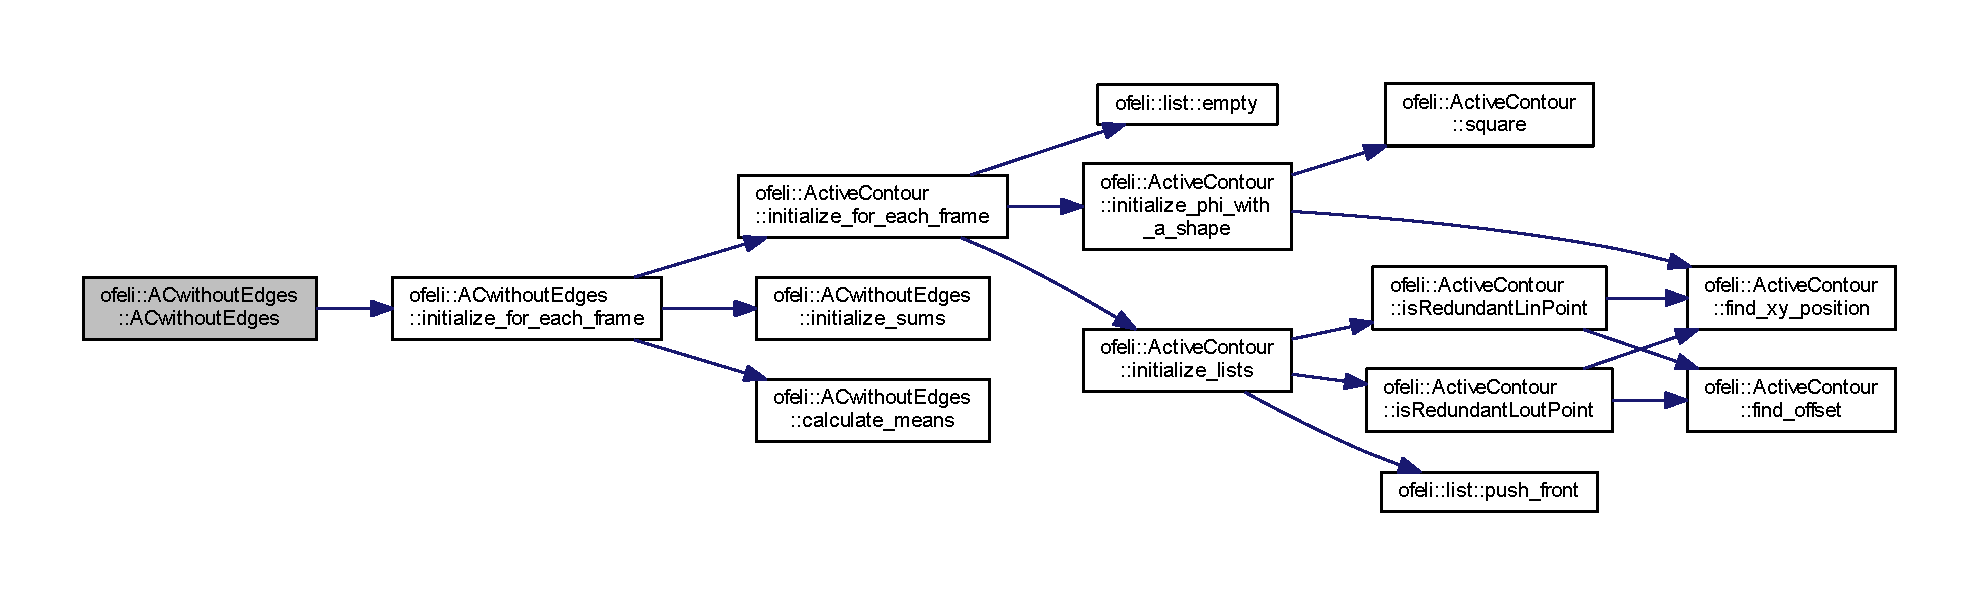
\includegraphics[width=350pt]{classofeli_1_1_a_cwithout_edges_ad3be07385b0a0d693036ddee99bdaf2b_cgraph}
\end{center}
\end{figure}


\hypertarget{classofeli_1_1_a_cwithout_edges_a3aafada5bffe3d4251ff22cd22ebb401}{\index{ofeli\-::\-A\-Cwithout\-Edges@{ofeli\-::\-A\-Cwithout\-Edges}!A\-Cwithout\-Edges@{A\-Cwithout\-Edges}}
\index{A\-Cwithout\-Edges@{A\-Cwithout\-Edges}!ofeli::ACwithoutEdges@{ofeli\-::\-A\-Cwithout\-Edges}}
\subsubsection[{A\-Cwithout\-Edges}]{\setlength{\rightskip}{0pt plus 5cm}A\-Cwithout\-Edges\-::\-A\-Cwithout\-Edges (
\begin{DoxyParamCaption}
\item[{const unsigned char $\ast$}]{img\-\_\-data1, }
\item[{int}]{img\-\_\-width1, }
\item[{int}]{img\-\_\-height1, }
\item[{const char $\ast$}]{phi\-\_\-init1, }
\item[{bool}]{has\-Cycle2\-\_\-1, }
\item[{int}]{kernel\-\_\-length1, }
\item[{double}]{sigma1, }
\item[{int}]{Na1, }
\item[{int}]{Ns1, }
\item[{int}]{lambda\-\_\-out1, }
\item[{int}]{lambda\-\_\-in1}
\end{DoxyParamCaption}
)}}\label{classofeli_1_1_a_cwithout_edges_a3aafada5bffe3d4251ff22cd22ebb401}


Constructor to initialize the active contour from an initial phi level-\/set function. 


\begin{DoxyParams}{Parameters}
{\em img\-\_\-data1} & Input pointer on the grayscale image data buffer. This buffer must be row-\/wise. Passed to \hyperlink{classofeli_1_1_active_contour_a96480d79e9a60817925903da233a5b1e}{img\-\_\-data}. \\
\hline
{\em img\-\_\-width1} & Image width, i.\-e. number of columns. Passed to \hyperlink{classofeli_1_1_active_contour_a3623de7ebc0d27ba7fac21a5929afbc6}{img\-\_\-width}. \\
\hline
{\em img\-\_\-height1} & Image height, i.\-e. number of rows. Passed to \hyperlink{classofeli_1_1_active_contour_a88d02b47bab737ec97fe3a7ea9554c0c}{img\-\_\-height}. \\
\hline
{\em phi\-\_\-init1} & Pointer on the initialized level-\/set function buffer. Copied to \hyperlink{classofeli_1_1_active_contour_aacb03a6ded4ca51cb52f58aeff955ef7}{phi}. \\
\hline
{\em has\-Cycle2\-\_\-1} & Boolean to have or not the curve smoothing, evolutions in the cycle 2 with an internal speed {\itshape Fint}. Passed to \hyperlink{classofeli_1_1_active_contour_aa763ff1bed211faa444013cbd5de0be3}{has\-Cycle2}. \\
\hline
{\em kernel\-\_\-length1} & Kernel length of the gaussian filter for the curve smoothing. \\
\hline
{\em sigma1} & Standard deviation of the gaussian kernel for the curve smoothing. \\
\hline
{\em Na1} & Number of times the active contour evolves in the cycle 1, external or data dependant evolutions with {\itshape Fd} speed. Passed to \hyperlink{classofeli_1_1_active_contour_a811a28ec9c39400d244783a8a2fe7e2d}{Na\-\_\-max}. \\
\hline
{\em Ns1} & Number of times the active contour evolves in the cycle 2, curve smoothing or internal evolutions with {\itshape Fint} speed. Passed to \hyperlink{classofeli_1_1_active_contour_a908322f93a50ce7808960236478649fe}{Ns\-\_\-max}. \\
\hline
{\em lambda\-\_\-out1} & Weight of the outside homogeneity criterion. Passed to \hyperlink{classofeli_1_1_a_cwithout_edges_a94489baa2bd0a04b86020e61de55680d}{lambda\-\_\-out}. \\
\hline
{\em lambda\-\_\-in1} & Weight of the inside homogeneity criterion. Passed to \hyperlink{classofeli_1_1_a_cwithout_edges_a43a550a7ba56e0b0861d120e47c96d95}{lambda\-\_\-in}. \\
\hline
\end{DoxyParams}


Definition at line 69 of file ac\-\_\-withoutedges.\-cpp.



Here is the call graph for this function\-:\nopagebreak
\begin{figure}[H]
\begin{center}
\leavevmode
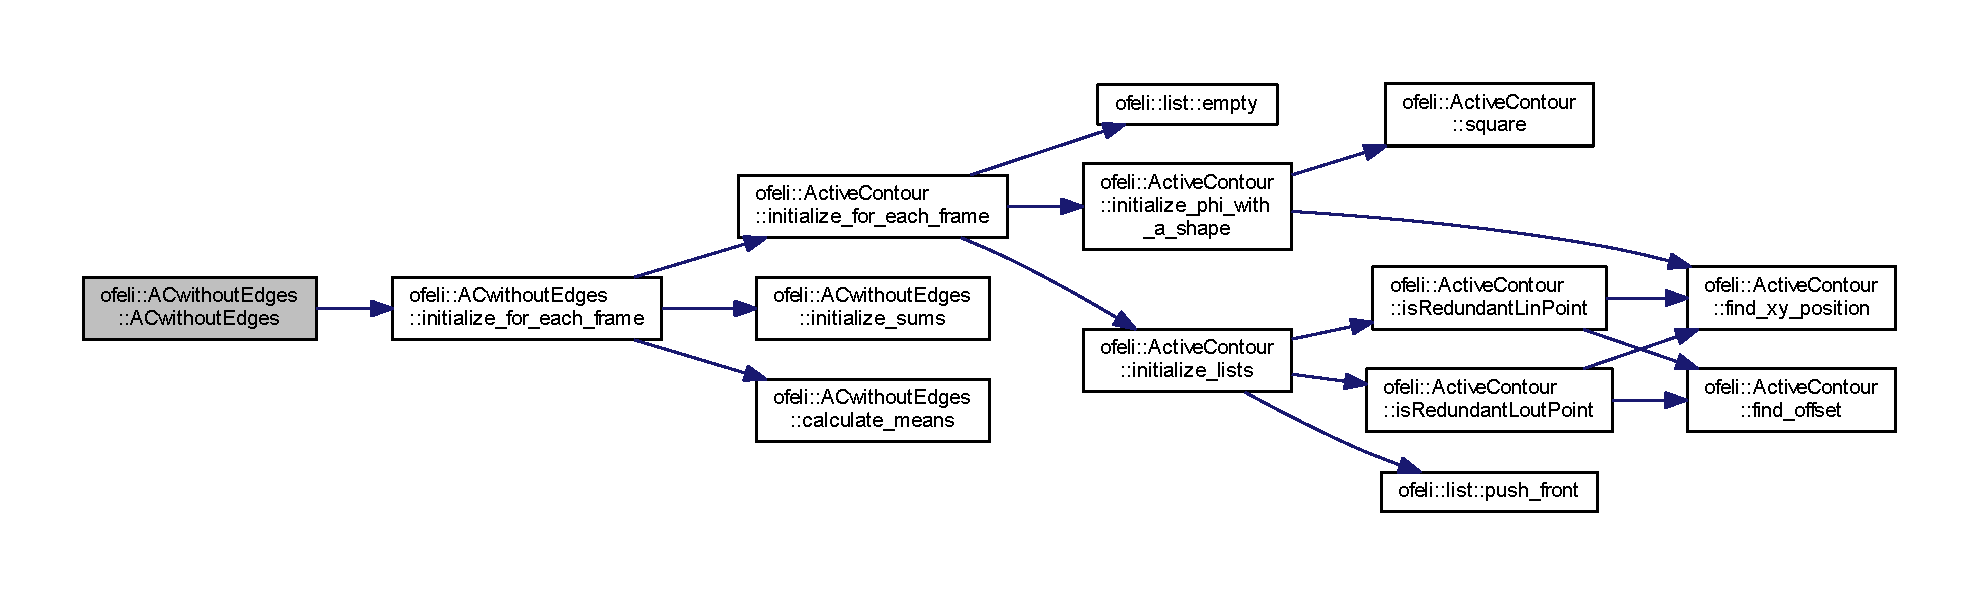
\includegraphics[width=350pt]{classofeli_1_1_a_cwithout_edges_a3aafada5bffe3d4251ff22cd22ebb401_cgraph}
\end{center}
\end{figure}




\subsection{Member Function Documentation}
\hypertarget{classofeli_1_1_a_cwithout_edges_a4190840f934080ff6eb64fa48c993f98}{\index{ofeli\-::\-A\-Cwithout\-Edges@{ofeli\-::\-A\-Cwithout\-Edges}!compute\-\_\-external\-\_\-speed\-\_\-\-Fd@{compute\-\_\-external\-\_\-speed\-\_\-\-Fd}}
\index{compute\-\_\-external\-\_\-speed\-\_\-\-Fd@{compute\-\_\-external\-\_\-speed\-\_\-\-Fd}!ofeli::ACwithoutEdges@{ofeli\-::\-A\-Cwithout\-Edges}}
\subsubsection[{compute\-\_\-external\-\_\-speed\-\_\-\-Fd}]{\setlength{\rightskip}{0pt plus 5cm}void A\-Cwithout\-Edges\-::compute\-\_\-external\-\_\-speed\-\_\-\-Fd (
\begin{DoxyParamCaption}
\item[{int}]{offset}
\end{DoxyParamCaption}
)\hspace{0.3cm}{\ttfamily [private]}, {\ttfamily [virtual]}}}\label{classofeli_1_1_a_cwithout_edges_a4190840f934080ff6eb64fa48c993f98}


Computes external speed {\itshape Fd} with the Chan-\/\-Vese model for a current point {\itshape }(x,y) of \hyperlink{classofeli_1_1_active_contour_a31e0eb18a7ea6ae90acf66ed018fcd85}{Lout} or \hyperlink{classofeli_1_1_active_contour_a7662d4f5c8b87d3e642b08b7e341bd79}{Lin}. 


\begin{DoxyParams}{Parameters}
{\em offset} & offset of the image data buffer with {\itshape offset} = {\itshape x} + {\itshape y} × \hyperlink{classofeli_1_1_active_contour_a3623de7ebc0d27ba7fac21a5929afbc6}{img\-\_\-width} \\
\hline
\end{DoxyParams}


Reimplemented from \hyperlink{classofeli_1_1_active_contour_ae3871b40f2f3e27ae0d75775798cdee1}{ofeli\-::\-Active\-Contour}.



Definition at line 140 of file ac\-\_\-withoutedges.\-cpp.



Here is the call graph for this function\-:\nopagebreak
\begin{figure}[H]
\begin{center}
\leavevmode
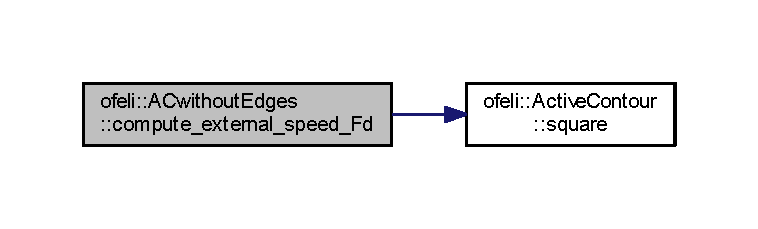
\includegraphics[width=350pt]{classofeli_1_1_a_cwithout_edges_a4190840f934080ff6eb64fa48c993f98_cgraph}
\end{center}
\end{figure}


\hypertarget{classofeli_1_1_a_cwithout_edges_aae62ec3548eb47ca5f67c2ede19a251b}{\index{ofeli\-::\-A\-Cwithout\-Edges@{ofeli\-::\-A\-Cwithout\-Edges}!updates\-\_\-for\-\_\-means\-\_\-in2@{updates\-\_\-for\-\_\-means\-\_\-in2}}
\index{updates\-\_\-for\-\_\-means\-\_\-in2@{updates\-\_\-for\-\_\-means\-\_\-in2}!ofeli::ACwithoutEdges@{ofeli\-::\-A\-Cwithout\-Edges}}
\subsubsection[{updates\-\_\-for\-\_\-means\-\_\-in2}]{\setlength{\rightskip}{0pt plus 5cm}void A\-Cwithout\-Edges\-::updates\-\_\-for\-\_\-means\-\_\-in2 (
\begin{DoxyParamCaption}
\item[{int}]{offset}
\end{DoxyParamCaption}
)\hspace{0.3cm}{\ttfamily [private]}, {\ttfamily [virtual]}}}\label{classofeli_1_1_a_cwithout_edges_aae62ec3548eb47ca5f67c2ede19a251b}


Updates variables \hyperlink{classofeli_1_1_a_cwithout_edges_a14f61eabccbac71bf616674e8feb44f5}{sum\-\_\-in}, \hyperlink{classofeli_1_1_a_cwithout_edges_a799b4078bc22cbde48cc29c93727efc5}{sum\-\_\-out}, \hyperlink{classofeli_1_1_a_cwithout_edges_a8d2c28710176ae9b562b4001f8171348}{n\-\_\-in} and \hyperlink{classofeli_1_1_a_cwithout_edges_a07818e5c3700b0164037e982077de10c}{n\-\_\-out}, before each \hyperlink{classofeli_1_1_active_contour_a7d9a557b580af708155ff4ab8bbfd73b}{switch\-\_\-in}, in the cycle 2, in order to calculate means \hyperlink{classofeli_1_1_a_cwithout_edges_a02c32b73dcc676251330a42b6fb4e6f4}{Cout} and \hyperlink{classofeli_1_1_a_cwithout_edges_af26f696be73588b2a150c3eef6f62c85}{Cin}. 


\begin{DoxyParams}{Parameters}
{\em offset} & offset of the image data buffer with {\itshape offset} = {\itshape x} + {\itshape y} × \hyperlink{classofeli_1_1_active_contour_a3623de7ebc0d27ba7fac21a5929afbc6}{img\-\_\-width} \\
\hline
\end{DoxyParams}


Reimplemented from \hyperlink{classofeli_1_1_active_contour_a77e9dc7bcbd0ba48499a499891e021cb}{ofeli\-::\-Active\-Contour}.



Definition at line 169 of file ac\-\_\-withoutedges.\-cpp.



Here is the call graph for this function\-:\nopagebreak
\begin{figure}[H]
\begin{center}
\leavevmode
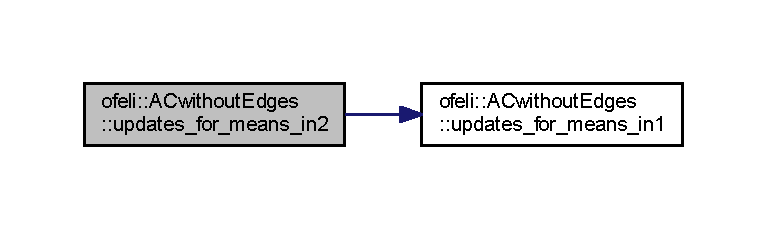
\includegraphics[width=350pt]{classofeli_1_1_a_cwithout_edges_aae62ec3548eb47ca5f67c2ede19a251b_cgraph}
\end{center}
\end{figure}


\hypertarget{classofeli_1_1_a_cwithout_edges_a80021d0ca688f3cbf46bccc870706e4c}{\index{ofeli\-::\-A\-Cwithout\-Edges@{ofeli\-::\-A\-Cwithout\-Edges}!updates\-\_\-for\-\_\-means\-\_\-out2@{updates\-\_\-for\-\_\-means\-\_\-out2}}
\index{updates\-\_\-for\-\_\-means\-\_\-out2@{updates\-\_\-for\-\_\-means\-\_\-out2}!ofeli::ACwithoutEdges@{ofeli\-::\-A\-Cwithout\-Edges}}
\subsubsection[{updates\-\_\-for\-\_\-means\-\_\-out2}]{\setlength{\rightskip}{0pt plus 5cm}void A\-Cwithout\-Edges\-::updates\-\_\-for\-\_\-means\-\_\-out2 (
\begin{DoxyParamCaption}
\item[{int}]{offset}
\end{DoxyParamCaption}
)\hspace{0.3cm}{\ttfamily [private]}, {\ttfamily [virtual]}}}\label{classofeli_1_1_a_cwithout_edges_a80021d0ca688f3cbf46bccc870706e4c}


Updates variables \hyperlink{classofeli_1_1_a_cwithout_edges_a14f61eabccbac71bf616674e8feb44f5}{sum\-\_\-in}, \hyperlink{classofeli_1_1_a_cwithout_edges_a799b4078bc22cbde48cc29c93727efc5}{sum\-\_\-out}, \hyperlink{classofeli_1_1_a_cwithout_edges_a8d2c28710176ae9b562b4001f8171348}{n\-\_\-in} and \hyperlink{classofeli_1_1_a_cwithout_edges_a07818e5c3700b0164037e982077de10c}{n\-\_\-out}, before each \hyperlink{classofeli_1_1_active_contour_a98af656dfc038e6f03c9e4bb67e39bd0}{switch\-\_\-out}, in the cycle 2, in order to calculate means \hyperlink{classofeli_1_1_a_cwithout_edges_a02c32b73dcc676251330a42b6fb4e6f4}{Cout} and \hyperlink{classofeli_1_1_a_cwithout_edges_af26f696be73588b2a150c3eef6f62c85}{Cin}. 


\begin{DoxyParams}{Parameters}
{\em offset} & offset of the image data buffer with {\itshape offset} = {\itshape x} + {\itshape y} × \hyperlink{classofeli_1_1_active_contour_a3623de7ebc0d27ba7fac21a5929afbc6}{img\-\_\-width} \\
\hline
\end{DoxyParams}


Reimplemented from \hyperlink{classofeli_1_1_active_contour_a347e650493750ad29b8b73ed52bdcf7a}{ofeli\-::\-Active\-Contour}.



Definition at line 178 of file ac\-\_\-withoutedges.\-cpp.



Here is the call graph for this function\-:\nopagebreak
\begin{figure}[H]
\begin{center}
\leavevmode
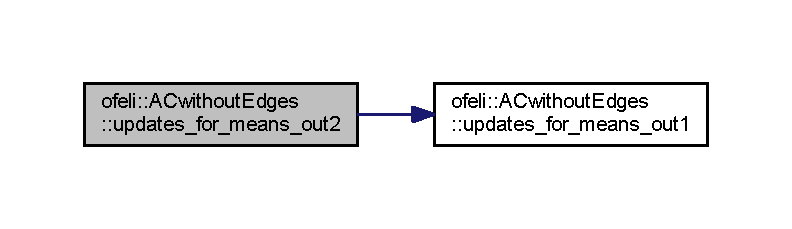
\includegraphics[width=350pt]{classofeli_1_1_a_cwithout_edges_a80021d0ca688f3cbf46bccc870706e4c_cgraph}
\end{center}
\end{figure}




The documentation for this class was generated from the following files\-:\begin{DoxyCompactItemize}
\item 
ac\-\_\-withoutedges.\-hpp\item 
ac\-\_\-withoutedges.\-cpp\end{DoxyCompactItemize}

\hypertarget{classofeli_1_1_a_cwithout_edges_y_u_v}{\section{ofeli\-:\-:A\-Cwithout\-Edges\-Y\-U\-V Class Reference}
\label{classofeli_1_1_a_cwithout_edges_y_u_v}\index{ofeli\-::\-A\-Cwithout\-Edges\-Y\-U\-V@{ofeli\-::\-A\-Cwithout\-Edges\-Y\-U\-V}}
}


{\ttfamily \#include $<$ac\-\_\-withoutedges\-\_\-yuv.\-hpp$>$}



Inheritance diagram for ofeli\-:\-:A\-Cwithout\-Edges\-Y\-U\-V\-:\nopagebreak
\begin{figure}[H]
\begin{center}
\leavevmode
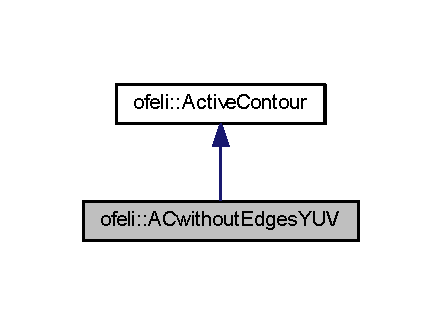
\includegraphics[width=212pt]{classofeli_1_1_a_cwithout_edges_y_u_v__inherit__graph}
\end{center}
\end{figure}


Collaboration diagram for ofeli\-:\-:A\-Cwithout\-Edges\-Y\-U\-V\-:\nopagebreak
\begin{figure}[H]
\begin{center}
\leavevmode
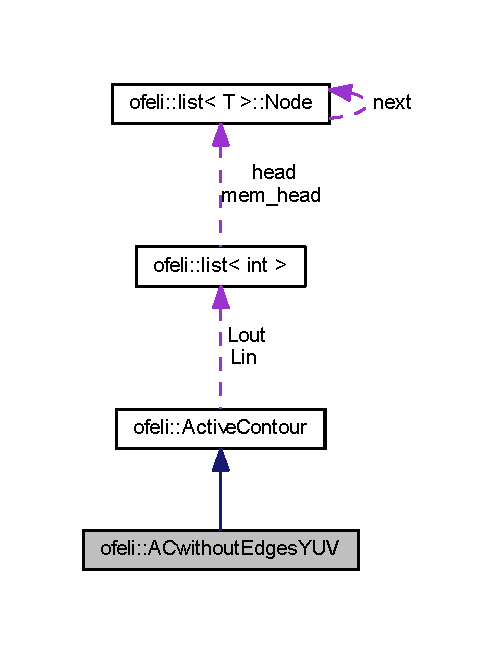
\includegraphics[width=238pt]{classofeli_1_1_a_cwithout_edges_y_u_v__coll__graph}
\end{center}
\end{figure}
\subsection*{Public Member Functions}
\begin{DoxyCompactItemize}
\item 
\hypertarget{classofeli_1_1_a_cwithout_edges_y_u_v_a80d0dc7b755e098cf08f1e155ec3e685}{\hyperlink{classofeli_1_1_a_cwithout_edges_y_u_v_a80d0dc7b755e098cf08f1e155ec3e685}{A\-Cwithout\-Edges\-Y\-U\-V} (const unsigned char $\ast$img\-\_\-rgb\-\_\-data1, int img\-\_\-width1, int img\-\_\-height1)}\label{classofeli_1_1_a_cwithout_edges_y_u_v_a80d0dc7b755e098cf08f1e155ec3e685}

\begin{DoxyCompactList}\small\item\em Constructor to initialize the active contour with a centered rectangle and the default values of the algorithm parameters. \end{DoxyCompactList}\item 
\hyperlink{classofeli_1_1_a_cwithout_edges_y_u_v_a31765b6ebe4825cc2a1ea815d1235c22}{A\-Cwithout\-Edges\-Y\-U\-V} (const unsigned char $\ast$img\-\_\-rgb\-\_\-data1, int img\-\_\-width1, int img\-\_\-height1, bool has\-Ellipse1, double init\-\_\-width1, double init\-\_\-height1, double center\-\_\-x1, double center\-\_\-y1, bool has\-Cycle2\-\_\-1, int kernel\-\_\-length1, double sigma1, int Na1, int Ns1, int lambda\-\_\-out1, int lambda\-\_\-in1, int alpha1, int beta1, int gamma1)
\begin{DoxyCompactList}\small\item\em Constructor to initialize the active contour from geometrical parameters of an unique shape, an ellipse or a rectangle. \end{DoxyCompactList}\item 
\hyperlink{classofeli_1_1_a_cwithout_edges_y_u_v_a63c5bcb0da045d930be9be686c5f5245}{A\-Cwithout\-Edges\-Y\-U\-V} (const unsigned char $\ast$img\-\_\-rgb\-\_\-data1, int img\-\_\-width1, int img\-\_\-height1, const char $\ast$phi\-\_\-init1, bool has\-Cycle2\-\_\-1, int kernel\-\_\-length1, double sigma1, int Na1, int Ns1, int lambda\-\_\-out1, int lambda\-\_\-in1, int alpha1, int beta1, int gamma1)
\begin{DoxyCompactList}\small\item\em Constructor to initialize the active contour from an initial phi level-\/set function. \end{DoxyCompactList}\item 
\hypertarget{classofeli_1_1_a_cwithout_edges_y_u_v_af4dc029288e6d49b6ac9c5a506a6b746}{\hyperlink{classofeli_1_1_a_cwithout_edges_y_u_v_af4dc029288e6d49b6ac9c5a506a6b746}{A\-Cwithout\-Edges\-Y\-U\-V} (const \hyperlink{classofeli_1_1_a_cwithout_edges_y_u_v}{A\-Cwithout\-Edges\-Y\-U\-V} \&ac)}\label{classofeli_1_1_a_cwithout_edges_y_u_v_af4dc029288e6d49b6ac9c5a506a6b746}

\begin{DoxyCompactList}\small\item\em Copy constructor. \end{DoxyCompactList}\item 
\hypertarget{classofeli_1_1_a_cwithout_edges_y_u_v_ad24ef70875e3435c524cb1385c3c43d3}{virtual void \hyperlink{classofeli_1_1_a_cwithout_edges_y_u_v_ad24ef70875e3435c524cb1385c3c43d3}{initialize\-\_\-for\-\_\-each\-\_\-frame} ()}\label{classofeli_1_1_a_cwithout_edges_y_u_v_ad24ef70875e3435c524cb1385c3c43d3}

\begin{DoxyCompactList}\small\item\em Initialization for each new frame buffer, used for video tracking. \end{DoxyCompactList}\item 
\hypertarget{classofeli_1_1_a_cwithout_edges_y_u_v_a27259e0b651cc835fd9eb0285ee0f2f3}{int \hyperlink{classofeli_1_1_a_cwithout_edges_y_u_v_a27259e0b651cc835fd9eb0285ee0f2f3}{get\-\_\-\-Cout\-R} () const }\label{classofeli_1_1_a_cwithout_edges_y_u_v_a27259e0b651cc835fd9eb0285ee0f2f3}

\begin{DoxyCompactList}\small\item\em Getter function for \hyperlink{classofeli_1_1_a_cwithout_edges_y_u_v_a6d5f27cda390c51891165958613a0e19}{Cout\-R}. \end{DoxyCompactList}\item 
\hypertarget{classofeli_1_1_a_cwithout_edges_y_u_v_a4b501d61dfea61cb63ef5799d75215fd}{int \hyperlink{classofeli_1_1_a_cwithout_edges_y_u_v_a4b501d61dfea61cb63ef5799d75215fd}{get\-\_\-\-Cout\-G} () const }\label{classofeli_1_1_a_cwithout_edges_y_u_v_a4b501d61dfea61cb63ef5799d75215fd}

\begin{DoxyCompactList}\small\item\em Getter function for \hyperlink{classofeli_1_1_a_cwithout_edges_y_u_v_a7204eb013515fad29ae5248219803225}{Cout\-G}. \end{DoxyCompactList}\item 
\hypertarget{classofeli_1_1_a_cwithout_edges_y_u_v_ae2abe7f7808159770231689922fbad88}{int \hyperlink{classofeli_1_1_a_cwithout_edges_y_u_v_ae2abe7f7808159770231689922fbad88}{get\-\_\-\-Cout\-B} () const }\label{classofeli_1_1_a_cwithout_edges_y_u_v_ae2abe7f7808159770231689922fbad88}

\begin{DoxyCompactList}\small\item\em Getter function for \hyperlink{classofeli_1_1_a_cwithout_edges_y_u_v_a74c6d6e79c6360ff67fa6402b44ddfc8}{Cout\-B}. \end{DoxyCompactList}\item 
\hypertarget{classofeli_1_1_a_cwithout_edges_y_u_v_a6059683b3761306d4155f11e39cfb6bd}{int \hyperlink{classofeli_1_1_a_cwithout_edges_y_u_v_a6059683b3761306d4155f11e39cfb6bd}{get\-\_\-\-Cin\-R} () const }\label{classofeli_1_1_a_cwithout_edges_y_u_v_a6059683b3761306d4155f11e39cfb6bd}

\begin{DoxyCompactList}\small\item\em Getter function for \hyperlink{classofeli_1_1_a_cwithout_edges_y_u_v_a530187c61ecd52f7205c31092717adbd}{Cin\-R}. \end{DoxyCompactList}\item 
\hypertarget{classofeli_1_1_a_cwithout_edges_y_u_v_aad7e64a5c29fa9adb9353f4667e30caf}{int \hyperlink{classofeli_1_1_a_cwithout_edges_y_u_v_aad7e64a5c29fa9adb9353f4667e30caf}{get\-\_\-\-Cin\-G} () const }\label{classofeli_1_1_a_cwithout_edges_y_u_v_aad7e64a5c29fa9adb9353f4667e30caf}

\begin{DoxyCompactList}\small\item\em Getter function for \hyperlink{classofeli_1_1_a_cwithout_edges_y_u_v_ac3fc93827ad0ab1513ff0b740d654106}{Cin\-G}. \end{DoxyCompactList}\item 
\hypertarget{classofeli_1_1_a_cwithout_edges_y_u_v_a388c2919ea7a3c0f7f31f590560e2c41}{int \hyperlink{classofeli_1_1_a_cwithout_edges_y_u_v_a388c2919ea7a3c0f7f31f590560e2c41}{get\-\_\-\-Cin\-B} () const }\label{classofeli_1_1_a_cwithout_edges_y_u_v_a388c2919ea7a3c0f7f31f590560e2c41}

\begin{DoxyCompactList}\small\item\em Getter function for \hyperlink{classofeli_1_1_a_cwithout_edges_y_u_v_a72114f3223a47ba7d688f0c755aa4ae8}{Cin\-B}. \end{DoxyCompactList}\item 
\hypertarget{classofeli_1_1_a_cwithout_edges_y_u_v_af86f85ff01de34d3125d90f3e50ce45d}{const int $\ast$ \hyperlink{classofeli_1_1_a_cwithout_edges_y_u_v_af86f85ff01de34d3125d90f3e50ce45d}{get\-\_\-\-Cout\-Y\-U\-V} () const }\label{classofeli_1_1_a_cwithout_edges_y_u_v_af86f85ff01de34d3125d90f3e50ce45d}

\begin{DoxyCompactList}\small\item\em Getter function for \hyperlink{classofeli_1_1_a_cwithout_edges_y_u_v_a1aea515bf36ea9f426cc653802252ce5}{Cout\-Y\-U\-V}. \end{DoxyCompactList}\item 
\hypertarget{classofeli_1_1_a_cwithout_edges_y_u_v_a1d9d8bb3e6ca6d92654399a88322641b}{const int $\ast$ \hyperlink{classofeli_1_1_a_cwithout_edges_y_u_v_a1d9d8bb3e6ca6d92654399a88322641b}{get\-\_\-\-Cin\-Y\-U\-V} () const }\label{classofeli_1_1_a_cwithout_edges_y_u_v_a1d9d8bb3e6ca6d92654399a88322641b}

\begin{DoxyCompactList}\small\item\em Getter function for \hyperlink{classofeli_1_1_a_cwithout_edges_y_u_v_ac5976def2629d484df763de752bb165d}{Cin\-Y\-U\-V}. \end{DoxyCompactList}\end{DoxyCompactItemize}
\subsection*{Private Member Functions}
\begin{DoxyCompactItemize}
\item 
\hypertarget{classofeli_1_1_a_cwithout_edges_y_u_v_a7913716e6f12f0020909fd1ff42149f4}{void \hyperlink{classofeli_1_1_a_cwithout_edges_y_u_v_a7913716e6f12f0020909fd1ff42149f4}{R\-G\-B\-\_\-from\-\_\-buffer} (int offset)}\label{classofeli_1_1_a_cwithout_edges_y_u_v_a7913716e6f12f0020909fd1ff42149f4}

\begin{DoxyCompactList}\small\item\em Affects the variable R, G, B from the buffer img\-\_\-rgb\-\_\-data. \end{DoxyCompactList}\item 
\hypertarget{classofeli_1_1_a_cwithout_edges_y_u_v_a68356b357307d95e2b431bb46c0223bb}{void \hyperlink{classofeli_1_1_a_cwithout_edges_y_u_v_a68356b357307d95e2b431bb46c0223bb}{initialize\-\_\-sums} ()}\label{classofeli_1_1_a_cwithout_edges_y_u_v_a68356b357307d95e2b431bb46c0223bb}

\begin{DoxyCompactList}\small\item\em Initializes the six sums and \hyperlink{classofeli_1_1_a_cwithout_edges_y_u_v_a63542bb13e9dd879714b6c71cd5fe62c}{n\-\_\-in} and \hyperlink{classofeli_1_1_a_cwithout_edges_y_u_v_a034adbc67a268bd84539fe8e76b9deec}{n\-\_\-out} with scanning through the image. \end{DoxyCompactList}\item 
\hypertarget{classofeli_1_1_a_cwithout_edges_y_u_v_ae8904a4a32fa48696641066ec5ae571d}{virtual void \hyperlink{classofeli_1_1_a_cwithout_edges_y_u_v_ae8904a4a32fa48696641066ec5ae571d}{calculate\-\_\-means} ()}\label{classofeli_1_1_a_cwithout_edges_y_u_v_ae8904a4a32fa48696641066ec5ae571d}

\begin{DoxyCompactList}\small\item\em Calculates means \hyperlink{classofeli_1_1_a_cwithout_edges_y_u_v_a1aea515bf36ea9f426cc653802252ce5}{Cout\-Y\-U\-V} and \hyperlink{classofeli_1_1_a_cwithout_edges_y_u_v_ac5976def2629d484df763de752bb165d}{Cin\-Y\-U\-V} in {\itshape O(1)} or accounting for the previous updates of (\hyperlink{classofeli_1_1_a_cwithout_edges_y_u_v_ad0f0935437296539710e4886afc94397}{sum\-\_\-out\-\_\-\-R}, \hyperlink{classofeli_1_1_a_cwithout_edges_y_u_v_a5ac2c58a2f10125ee7c2c21e80a321cc}{sum\-\_\-out\-\_\-\-G}, \hyperlink{classofeli_1_1_a_cwithout_edges_y_u_v_a978f68f2ac215e14c532cf794ce46881}{sum\-\_\-out\-\_\-\-B}) and (\hyperlink{classofeli_1_1_a_cwithout_edges_y_u_v_aba49728a621675acf3279f38134afc1f}{sum\-\_\-in\-\_\-\-R}, \hyperlink{classofeli_1_1_a_cwithout_edges_y_u_v_aa9a1b8f6a101ea6f016ad318e780e7a4}{sum\-\_\-in\-\_\-\-G}, \hyperlink{classofeli_1_1_a_cwithout_edges_y_u_v_aee9f33db9baf2e45063258250090f68c}{sum\-\_\-in\-\_\-\-B}), in {\itshape O}(\hyperlink{classofeli_1_1_active_contour_aefe0738d8a43f3981d591a0cc78ed717}{lists\-\_\-length}) and not in {\itshape O}(\hyperlink{classofeli_1_1_active_contour_a9182e11132f64d7607fbd19a78f58387}{img\-\_\-size}). \end{DoxyCompactList}\item 
virtual int \hyperlink{classofeli_1_1_a_cwithout_edges_y_u_v_ae61e98ace069646a009de7cd7148e065}{compute\-\_\-external\-\_\-speed\-\_\-\-Fd} (int offset)
\begin{DoxyCompactList}\small\item\em Computes external speed {\itshape Fd} with the Chan-\/\-Vese model for a current point {\itshape }(x,y) of \hyperlink{classofeli_1_1_active_contour_a31e0eb18a7ea6ae90acf66ed018fcd85}{Lout} or \hyperlink{classofeli_1_1_active_contour_a7662d4f5c8b87d3e642b08b7e341bd79}{Lin}. \end{DoxyCompactList}\item 
\hypertarget{classofeli_1_1_a_cwithout_edges_y_u_v_a35e76dc7dc884e9d40f69aa3f011890a}{virtual void \hyperlink{classofeli_1_1_a_cwithout_edges_y_u_v_a35e76dc7dc884e9d40f69aa3f011890a}{updates\-\_\-for\-\_\-means\-\_\-in1} ()}\label{classofeli_1_1_a_cwithout_edges_y_u_v_a35e76dc7dc884e9d40f69aa3f011890a}

\begin{DoxyCompactList}\small\item\em Updates the six sums, \hyperlink{classofeli_1_1_a_cwithout_edges_y_u_v_a63542bb13e9dd879714b6c71cd5fe62c}{n\-\_\-in} and \hyperlink{classofeli_1_1_a_cwithout_edges_y_u_v_a034adbc67a268bd84539fe8e76b9deec}{n\-\_\-out}, before each \hyperlink{classofeli_1_1_active_contour_a7d9a557b580af708155ff4ab8bbfd73b}{switch\-\_\-in}, in the cycle 1, in order to calculate means \hyperlink{classofeli_1_1_a_cwithout_edges_y_u_v_a1aea515bf36ea9f426cc653802252ce5}{Cout\-Y\-U\-V} and \hyperlink{classofeli_1_1_a_cwithout_edges_y_u_v_ac5976def2629d484df763de752bb165d}{Cin\-Y\-U\-V}. \end{DoxyCompactList}\item 
\hypertarget{classofeli_1_1_a_cwithout_edges_y_u_v_a884eb5753c80701150b8be4699688e6b}{virtual void \hyperlink{classofeli_1_1_a_cwithout_edges_y_u_v_a884eb5753c80701150b8be4699688e6b}{updates\-\_\-for\-\_\-means\-\_\-out1} ()}\label{classofeli_1_1_a_cwithout_edges_y_u_v_a884eb5753c80701150b8be4699688e6b}

\begin{DoxyCompactList}\small\item\em Updates the six sums, \hyperlink{classofeli_1_1_a_cwithout_edges_y_u_v_a63542bb13e9dd879714b6c71cd5fe62c}{n\-\_\-in} and \hyperlink{classofeli_1_1_a_cwithout_edges_y_u_v_a034adbc67a268bd84539fe8e76b9deec}{n\-\_\-out}, before each \hyperlink{classofeli_1_1_active_contour_a98af656dfc038e6f03c9e4bb67e39bd0}{switch\-\_\-out}, in the cycle 1, in order to calculate means \hyperlink{classofeli_1_1_a_cwithout_edges_y_u_v_a1aea515bf36ea9f426cc653802252ce5}{Cout\-Y\-U\-V} and \hyperlink{classofeli_1_1_a_cwithout_edges_y_u_v_ac5976def2629d484df763de752bb165d}{Cin\-Y\-U\-V}. \end{DoxyCompactList}\item 
virtual void \hyperlink{classofeli_1_1_a_cwithout_edges_y_u_v_a249aa0e9664cf4f024997ac4475fe70c}{updates\-\_\-for\-\_\-means\-\_\-in2} (int offset)
\begin{DoxyCompactList}\small\item\em Updates the six sums, \hyperlink{classofeli_1_1_a_cwithout_edges_y_u_v_a63542bb13e9dd879714b6c71cd5fe62c}{n\-\_\-in} and \hyperlink{classofeli_1_1_a_cwithout_edges_y_u_v_a034adbc67a268bd84539fe8e76b9deec}{n\-\_\-out}, before each \hyperlink{classofeli_1_1_active_contour_a7d9a557b580af708155ff4ab8bbfd73b}{switch\-\_\-in}, in the cycle 2, in order to calculate means \hyperlink{classofeli_1_1_a_cwithout_edges_y_u_v_a1aea515bf36ea9f426cc653802252ce5}{Cout\-Y\-U\-V} and \hyperlink{classofeli_1_1_a_cwithout_edges_y_u_v_ac5976def2629d484df763de752bb165d}{Cin\-Y\-U\-V}. \end{DoxyCompactList}\item 
virtual void \hyperlink{classofeli_1_1_a_cwithout_edges_y_u_v_a43b463f3b8d5cb9604fd73b18083409a}{updates\-\_\-for\-\_\-means\-\_\-out2} (int offset)
\begin{DoxyCompactList}\small\item\em Updates the six sums, \hyperlink{classofeli_1_1_a_cwithout_edges_y_u_v_a63542bb13e9dd879714b6c71cd5fe62c}{n\-\_\-in} and \hyperlink{classofeli_1_1_a_cwithout_edges_y_u_v_a034adbc67a268bd84539fe8e76b9deec}{n\-\_\-out}, before each \hyperlink{classofeli_1_1_active_contour_a98af656dfc038e6f03c9e4bb67e39bd0}{switch\-\_\-out}, in the cycle 2, in order to calculate means \hyperlink{classofeli_1_1_a_cwithout_edges_y_u_v_a1aea515bf36ea9f426cc653802252ce5}{Cout\-Y\-U\-V} and \hyperlink{classofeli_1_1_a_cwithout_edges_y_u_v_ac5976def2629d484df763de752bb165d}{Cin\-Y\-U\-V}. \end{DoxyCompactList}\end{DoxyCompactItemize}
\subsection*{Static Private Member Functions}
\begin{DoxyCompactItemize}
\item 
\hypertarget{classofeli_1_1_a_cwithout_edges_y_u_v_a2db2c26b4add310859ba36d701834d81}{static void \hyperlink{classofeli_1_1_a_cwithout_edges_y_u_v_a2db2c26b4add310859ba36d701834d81}{calculate\-\_\-\-Y\-U\-V} (int \hyperlink{classofeli_1_1_a_cwithout_edges_y_u_v_a2590133637eb415a75ba848efb3d15d0}{R}, int \hyperlink{classofeli_1_1_a_cwithout_edges_y_u_v_a39d9c82c2cebebd133d9aaa4faa2eef0}{G}, int \hyperlink{classofeli_1_1_a_cwithout_edges_y_u_v_af11928f0c101c0487b497b4249e5d5e4}{B}, int Y\-U\-V\mbox{[}$\,$\mbox{]})}\label{classofeli_1_1_a_cwithout_edges_y_u_v_a2db2c26b4add310859ba36d701834d81}

\begin{DoxyCompactList}\small\item\em Calculates {\itshape Y\-U\-V} value with a (\hyperlink{classofeli_1_1_a_cwithout_edges_y_u_v_a2590133637eb415a75ba848efb3d15d0}{R},\hyperlink{classofeli_1_1_a_cwithout_edges_y_u_v_a39d9c82c2cebebd133d9aaa4faa2eef0}{G},\hyperlink{classofeli_1_1_a_cwithout_edges_y_u_v_af11928f0c101c0487b497b4249e5d5e4}{B}) value. \end{DoxyCompactList}\end{DoxyCompactItemize}
\subsection*{Private Attributes}
\begin{DoxyCompactItemize}
\item 
\hypertarget{classofeli_1_1_a_cwithout_edges_y_u_v_a2590133637eb415a75ba848efb3d15d0}{int \hyperlink{classofeli_1_1_a_cwithout_edges_y_u_v_a2590133637eb415a75ba848efb3d15d0}{R}}\label{classofeli_1_1_a_cwithout_edges_y_u_v_a2590133637eb415a75ba848efb3d15d0}

\begin{DoxyCompactList}\small\item\em Red component of the current pixel. \end{DoxyCompactList}\item 
\hypertarget{classofeli_1_1_a_cwithout_edges_y_u_v_a39d9c82c2cebebd133d9aaa4faa2eef0}{int \hyperlink{classofeli_1_1_a_cwithout_edges_y_u_v_a39d9c82c2cebebd133d9aaa4faa2eef0}{G}}\label{classofeli_1_1_a_cwithout_edges_y_u_v_a39d9c82c2cebebd133d9aaa4faa2eef0}

\begin{DoxyCompactList}\small\item\em Green component of the current pixel. \end{DoxyCompactList}\item 
\hypertarget{classofeli_1_1_a_cwithout_edges_y_u_v_af11928f0c101c0487b497b4249e5d5e4}{int \hyperlink{classofeli_1_1_a_cwithout_edges_y_u_v_af11928f0c101c0487b497b4249e5d5e4}{B}}\label{classofeli_1_1_a_cwithout_edges_y_u_v_af11928f0c101c0487b497b4249e5d5e4}

\begin{DoxyCompactList}\small\item\em Blue component of the current pixel. \end{DoxyCompactList}\item 
\hypertarget{classofeli_1_1_a_cwithout_edges_y_u_v_a1aea515bf36ea9f426cc653802252ce5}{int \hyperlink{classofeli_1_1_a_cwithout_edges_y_u_v_a1aea515bf36ea9f426cc653802252ce5}{Cout\-Y\-U\-V} \mbox{[}3\mbox{]}}\label{classofeli_1_1_a_cwithout_edges_y_u_v_a1aea515bf36ea9f426cc653802252ce5}

\begin{DoxyCompactList}\small\item\em Y\-U\-V mean of the pixels outside the curve, i.\-e. pixels $i$ with $\phi \left( i\right) >0$ . \end{DoxyCompactList}\item 
\hypertarget{classofeli_1_1_a_cwithout_edges_y_u_v_ac5976def2629d484df763de752bb165d}{int \hyperlink{classofeli_1_1_a_cwithout_edges_y_u_v_ac5976def2629d484df763de752bb165d}{Cin\-Y\-U\-V} \mbox{[}3\mbox{]}}\label{classofeli_1_1_a_cwithout_edges_y_u_v_ac5976def2629d484df763de752bb165d}

\begin{DoxyCompactList}\small\item\em Y\-U\-V mean of the pixels inside the curve, i.\-e. pixels $i$ with $\phi \left( i\right) <0$ . \end{DoxyCompactList}\item 
\hypertarget{classofeli_1_1_a_cwithout_edges_y_u_v_a6d5f27cda390c51891165958613a0e19}{int \hyperlink{classofeli_1_1_a_cwithout_edges_y_u_v_a6d5f27cda390c51891165958613a0e19}{Cout\-R}}\label{classofeli_1_1_a_cwithout_edges_y_u_v_a6d5f27cda390c51891165958613a0e19}

\begin{DoxyCompactList}\small\item\em Mean of component {\itshape R} of the pixels outside the curve, i.\-e. pixels $i$ with $\phi \left( i\right) >0$ . \end{DoxyCompactList}\item 
\hypertarget{classofeli_1_1_a_cwithout_edges_y_u_v_a7204eb013515fad29ae5248219803225}{int \hyperlink{classofeli_1_1_a_cwithout_edges_y_u_v_a7204eb013515fad29ae5248219803225}{Cout\-G}}\label{classofeli_1_1_a_cwithout_edges_y_u_v_a7204eb013515fad29ae5248219803225}

\begin{DoxyCompactList}\small\item\em Mean of component {\itshape G} of the pixels outside the curve, i.\-e. pixels $i$ with $\phi \left( i\right) >0$ . \end{DoxyCompactList}\item 
\hypertarget{classofeli_1_1_a_cwithout_edges_y_u_v_a74c6d6e79c6360ff67fa6402b44ddfc8}{int \hyperlink{classofeli_1_1_a_cwithout_edges_y_u_v_a74c6d6e79c6360ff67fa6402b44ddfc8}{Cout\-B}}\label{classofeli_1_1_a_cwithout_edges_y_u_v_a74c6d6e79c6360ff67fa6402b44ddfc8}

\begin{DoxyCompactList}\small\item\em Mean of component {\itshape B} of the pixels outside the curve, i.\-e. pixels $i$ with $\phi \left( i\right) >0$ . \end{DoxyCompactList}\item 
\hypertarget{classofeli_1_1_a_cwithout_edges_y_u_v_a530187c61ecd52f7205c31092717adbd}{int \hyperlink{classofeli_1_1_a_cwithout_edges_y_u_v_a530187c61ecd52f7205c31092717adbd}{Cin\-R}}\label{classofeli_1_1_a_cwithout_edges_y_u_v_a530187c61ecd52f7205c31092717adbd}

\begin{DoxyCompactList}\small\item\em Mean of component {\itshape R} of the pixels inside the curve, i.\-e. pixels $i$ with $\phi \left( i\right) <0$ . \end{DoxyCompactList}\item 
\hypertarget{classofeli_1_1_a_cwithout_edges_y_u_v_ac3fc93827ad0ab1513ff0b740d654106}{int \hyperlink{classofeli_1_1_a_cwithout_edges_y_u_v_ac3fc93827ad0ab1513ff0b740d654106}{Cin\-G}}\label{classofeli_1_1_a_cwithout_edges_y_u_v_ac3fc93827ad0ab1513ff0b740d654106}

\begin{DoxyCompactList}\small\item\em Mean of component {\itshape G} of the pixels inside the curve, i.\-e. pixels $i$ with $\phi \left( i\right) <0$ . \end{DoxyCompactList}\item 
\hypertarget{classofeli_1_1_a_cwithout_edges_y_u_v_a72114f3223a47ba7d688f0c755aa4ae8}{int \hyperlink{classofeli_1_1_a_cwithout_edges_y_u_v_a72114f3223a47ba7d688f0c755aa4ae8}{Cin\-B}}\label{classofeli_1_1_a_cwithout_edges_y_u_v_a72114f3223a47ba7d688f0c755aa4ae8}

\begin{DoxyCompactList}\small\item\em Mean of component {\itshape B} of the pixels inside the curve, i.\-e. pixels $i$ with $\phi \left( i\right) <0$ . \end{DoxyCompactList}\item 
\hypertarget{classofeli_1_1_a_cwithout_edges_y_u_v_a613340fb017ff19af8510c9d72c9663b}{const int \hyperlink{classofeli_1_1_a_cwithout_edges_y_u_v_a613340fb017ff19af8510c9d72c9663b}{alpha}}\label{classofeli_1_1_a_cwithout_edges_y_u_v_a613340fb017ff19af8510c9d72c9663b}

\begin{DoxyCompactList}\small\item\em Weight of component {\itshape Y} to calculate external speed {\itshape Fd}. \end{DoxyCompactList}\item 
\hypertarget{classofeli_1_1_a_cwithout_edges_y_u_v_ae341898fb9f83bf41a731e1ada24cf0a}{const int \hyperlink{classofeli_1_1_a_cwithout_edges_y_u_v_ae341898fb9f83bf41a731e1ada24cf0a}{beta}}\label{classofeli_1_1_a_cwithout_edges_y_u_v_ae341898fb9f83bf41a731e1ada24cf0a}

\begin{DoxyCompactList}\small\item\em Weight of component {\itshape U} to calculate external speed {\itshape Fd}. \end{DoxyCompactList}\item 
\hypertarget{classofeli_1_1_a_cwithout_edges_y_u_v_a249bf1ba21819ddb9f63f0ceef8a97b2}{const int \hyperlink{classofeli_1_1_a_cwithout_edges_y_u_v_a249bf1ba21819ddb9f63f0ceef8a97b2}{gamma}}\label{classofeli_1_1_a_cwithout_edges_y_u_v_a249bf1ba21819ddb9f63f0ceef8a97b2}

\begin{DoxyCompactList}\small\item\em Weight of component {\itshape V} to calculate external speed {\itshape Fd}. \end{DoxyCompactList}\item 
\hypertarget{classofeli_1_1_a_cwithout_edges_y_u_v_a7e638b979761b49ad1aecc50a194dad0}{const int \hyperlink{classofeli_1_1_a_cwithout_edges_y_u_v_a7e638b979761b49ad1aecc50a194dad0}{lambda\-\_\-out}}\label{classofeli_1_1_a_cwithout_edges_y_u_v_a7e638b979761b49ad1aecc50a194dad0}

\begin{DoxyCompactList}\small\item\em Weight of the outside homogeneity criterion in the Chan-\/\-Vese model. \end{DoxyCompactList}\item 
\hypertarget{classofeli_1_1_a_cwithout_edges_y_u_v_a311f8c97d1fbdcdbb76b1b09aea59212}{const int \hyperlink{classofeli_1_1_a_cwithout_edges_y_u_v_a311f8c97d1fbdcdbb76b1b09aea59212}{lambda\-\_\-in}}\label{classofeli_1_1_a_cwithout_edges_y_u_v_a311f8c97d1fbdcdbb76b1b09aea59212}

\begin{DoxyCompactList}\small\item\em Weight of the inside homogeneity criterion in the Chan-\/\-Vese model. \end{DoxyCompactList}\item 
\hypertarget{classofeli_1_1_a_cwithout_edges_y_u_v_ad0f0935437296539710e4886afc94397}{int \hyperlink{classofeli_1_1_a_cwithout_edges_y_u_v_ad0f0935437296539710e4886afc94397}{sum\-\_\-out\-\_\-\-R}}\label{classofeli_1_1_a_cwithout_edges_y_u_v_ad0f0935437296539710e4886afc94397}

\begin{DoxyCompactList}\small\item\em Sum of component \hyperlink{classofeli_1_1_a_cwithout_edges_y_u_v_a2590133637eb415a75ba848efb3d15d0}{R} of the pixels outside the curve, i.\-e. pixels $i$ with $\phi \left( i\right) >0$ . \end{DoxyCompactList}\item 
\hypertarget{classofeli_1_1_a_cwithout_edges_y_u_v_aba49728a621675acf3279f38134afc1f}{int \hyperlink{classofeli_1_1_a_cwithout_edges_y_u_v_aba49728a621675acf3279f38134afc1f}{sum\-\_\-in\-\_\-\-R}}\label{classofeli_1_1_a_cwithout_edges_y_u_v_aba49728a621675acf3279f38134afc1f}

\begin{DoxyCompactList}\small\item\em Sum of component \hyperlink{classofeli_1_1_a_cwithout_edges_y_u_v_a2590133637eb415a75ba848efb3d15d0}{R} of the pixels intside the curve, i.\-e. pixels $i$ with $\phi \left( i\right) <0$ . \end{DoxyCompactList}\item 
\hypertarget{classofeli_1_1_a_cwithout_edges_y_u_v_a5ac2c58a2f10125ee7c2c21e80a321cc}{int \hyperlink{classofeli_1_1_a_cwithout_edges_y_u_v_a5ac2c58a2f10125ee7c2c21e80a321cc}{sum\-\_\-out\-\_\-\-G}}\label{classofeli_1_1_a_cwithout_edges_y_u_v_a5ac2c58a2f10125ee7c2c21e80a321cc}

\begin{DoxyCompactList}\small\item\em Sum of component \hyperlink{classofeli_1_1_a_cwithout_edges_y_u_v_a39d9c82c2cebebd133d9aaa4faa2eef0}{G} of the pixels outside the curve, i.\-e. pixels $i$ with $\phi \left( i\right) >0$ . \end{DoxyCompactList}\item 
\hypertarget{classofeli_1_1_a_cwithout_edges_y_u_v_aa9a1b8f6a101ea6f016ad318e780e7a4}{int \hyperlink{classofeli_1_1_a_cwithout_edges_y_u_v_aa9a1b8f6a101ea6f016ad318e780e7a4}{sum\-\_\-in\-\_\-\-G}}\label{classofeli_1_1_a_cwithout_edges_y_u_v_aa9a1b8f6a101ea6f016ad318e780e7a4}

\begin{DoxyCompactList}\small\item\em Sum of component \hyperlink{classofeli_1_1_a_cwithout_edges_y_u_v_a39d9c82c2cebebd133d9aaa4faa2eef0}{G} of the pixels intside the curve, i.\-e. pixels $i$ with $\phi \left( i\right) <0$ . \end{DoxyCompactList}\item 
\hypertarget{classofeli_1_1_a_cwithout_edges_y_u_v_a978f68f2ac215e14c532cf794ce46881}{int \hyperlink{classofeli_1_1_a_cwithout_edges_y_u_v_a978f68f2ac215e14c532cf794ce46881}{sum\-\_\-out\-\_\-\-B}}\label{classofeli_1_1_a_cwithout_edges_y_u_v_a978f68f2ac215e14c532cf794ce46881}

\begin{DoxyCompactList}\small\item\em Sum of component \hyperlink{classofeli_1_1_a_cwithout_edges_y_u_v_af11928f0c101c0487b497b4249e5d5e4}{B} of the pixels outside the curve, i.\-e. pixels $i$ with $\phi \left( i\right) >0$ . \end{DoxyCompactList}\item 
\hypertarget{classofeli_1_1_a_cwithout_edges_y_u_v_aee9f33db9baf2e45063258250090f68c}{int \hyperlink{classofeli_1_1_a_cwithout_edges_y_u_v_aee9f33db9baf2e45063258250090f68c}{sum\-\_\-in\-\_\-\-B}}\label{classofeli_1_1_a_cwithout_edges_y_u_v_aee9f33db9baf2e45063258250090f68c}

\begin{DoxyCompactList}\small\item\em Sum of component \hyperlink{classofeli_1_1_a_cwithout_edges_y_u_v_af11928f0c101c0487b497b4249e5d5e4}{B} of the pixels intside the curve, i.\-e. pixels $i$ with $\phi \left( i\right) <0$ . \end{DoxyCompactList}\item 
\hypertarget{classofeli_1_1_a_cwithout_edges_y_u_v_a034adbc67a268bd84539fe8e76b9deec}{int \hyperlink{classofeli_1_1_a_cwithout_edges_y_u_v_a034adbc67a268bd84539fe8e76b9deec}{n\-\_\-out}}\label{classofeli_1_1_a_cwithout_edges_y_u_v_a034adbc67a268bd84539fe8e76b9deec}

\begin{DoxyCompactList}\small\item\em Number of pixels outside the curve, i.\-e. pixels $i$ with $\phi \left( i\right) >0$ . \end{DoxyCompactList}\item 
\hypertarget{classofeli_1_1_a_cwithout_edges_y_u_v_a63542bb13e9dd879714b6c71cd5fe62c}{int \hyperlink{classofeli_1_1_a_cwithout_edges_y_u_v_a63542bb13e9dd879714b6c71cd5fe62c}{n\-\_\-in}}\label{classofeli_1_1_a_cwithout_edges_y_u_v_a63542bb13e9dd879714b6c71cd5fe62c}

\begin{DoxyCompactList}\small\item\em Number of pixels inside the curve, i.\-e. pixels $i$ with $\phi \left( i\right) <0$ . \end{DoxyCompactList}\end{DoxyCompactItemize}
\subsection*{Additional Inherited Members}


\subsection{Detailed Description}
The child class \hyperlink{classofeli_1_1_a_cwithout_edges_y_u_v}{A\-Cwithout\-Edges\-Y\-U\-V} implements a function to calculate specifically speed {\itshape Fd} based on the Chan-\/\-Vese model, a region-\/based energy functional. The regularization of our active contour is performed by a gaussian smoothing of \hyperlink{classofeli_1_1_active_contour_aacb03a6ded4ca51cb52f58aeff955ef7}{phi} so we are interested uniquely by the external or data dependant term of this energy functional.\par
 $F_{d}=\lambda _{out}\left[ \alpha \left( Y_{out}-C_{outC}\right) ^{2}+ \beta \left( U_{out}-C_{outU}\right) ^{2}+ \gamma \left( V_{out}-C_{outV}\right) ^{2}\right] + \lambda _{in}\left[ \alpha \left( Y_{in}-C_{inY}\right) ^{2}+ \beta \left( U_{in}-C_{inU}\right) ^{2}+ \gamma \left( V_{in}-C_{inV}\right) ^{2}\right]$
\begin{DoxyItemize}
\item $F_{d}$ \-: data dependant evolution speed calculated for each point of the active contour, only it sign is used by the algorithm. \par

\item $Y$ \-: luminance component Y of the (Y,U,V) color space of the current pixel of the active contour. \par

\item $U$ \-: chrominance component U of the (Y,U,V) color space of the current pixel of the active contour. \par

\item $V$ \-: chrominance component V of the (Y,U,V) color space of the current pixel of the active contour. \par

\item $C_{out}$ \-: mean of the intensities or grey-\/levels of the pixels outside the curve, i.\-e. pixels $i$ with $\phi \left( i\right) >0$. \par

\item $C_{in}$ \-: mean of the intensities or grey-\/levels of the pixels inside the curve, i.\-e. pixels $i$ with $\phi \left( i\right) <0$. \par

\item $C_{out}$ \-: mean of the intensities or grey-\/levels of the pixels outside the curve, i.\-e. pixels $i$ with $\phi \left( i\right) >0$. \par

\item $C_{in}$ \-: mean of the intensities or grey-\/levels of the pixels inside the curve, i.\-e. pixels $i$ with $\phi \left( i\right) <0$. \par

\item $C_{out}$ \-: mean of the intensities or grey-\/levels of the pixels outside the curve, i.\-e. pixels $i$ with $\phi \left( i\right) >0$. \par

\item $C_{in}$ \-: mean of the intensities or grey-\/levels of the pixels inside the curve, i.\-e. pixels $i$ with $\phi \left( i\right) <0$. \par

\item $\lambda _{out}$ \-: weight of the outside homogeneity criterion in the Chan-\/\-Vese model. \par

\item $\lambda _{in}$ \-: weight of the inside homogeneity criterion in the Chan-\/\-Vese model. \par

\item $\alpha$ \-: weight of the luminance component Y. \par

\item $\beta$ \-: weight of the chrominance component U. \par

\item $\gamma$ \-: weight of the chrominance component V. 
\end{DoxyItemize}

Definition at line 48 of file ac\-\_\-withoutedges\-\_\-yuv.\-hpp.



\subsection{Constructor \& Destructor Documentation}
\hypertarget{classofeli_1_1_a_cwithout_edges_y_u_v_a31765b6ebe4825cc2a1ea815d1235c22}{\index{ofeli\-::\-A\-Cwithout\-Edges\-Y\-U\-V@{ofeli\-::\-A\-Cwithout\-Edges\-Y\-U\-V}!A\-Cwithout\-Edges\-Y\-U\-V@{A\-Cwithout\-Edges\-Y\-U\-V}}
\index{A\-Cwithout\-Edges\-Y\-U\-V@{A\-Cwithout\-Edges\-Y\-U\-V}!ofeli::ACwithoutEdgesYUV@{ofeli\-::\-A\-Cwithout\-Edges\-Y\-U\-V}}
\subsubsection[{A\-Cwithout\-Edges\-Y\-U\-V}]{\setlength{\rightskip}{0pt plus 5cm}A\-Cwithout\-Edges\-Y\-U\-V\-::\-A\-Cwithout\-Edges\-Y\-U\-V (
\begin{DoxyParamCaption}
\item[{const unsigned char $\ast$}]{img\-\_\-rgb\-\_\-data1, }
\item[{int}]{img\-\_\-width1, }
\item[{int}]{img\-\_\-height1, }
\item[{bool}]{has\-Ellipse1, }
\item[{double}]{init\-\_\-width1, }
\item[{double}]{init\-\_\-height1, }
\item[{double}]{center\-\_\-x1, }
\item[{double}]{center\-\_\-y1, }
\item[{bool}]{has\-Cycle2\-\_\-1, }
\item[{int}]{kernel\-\_\-length1, }
\item[{double}]{sigma1, }
\item[{int}]{Na1, }
\item[{int}]{Ns1, }
\item[{int}]{lambda\-\_\-out1, }
\item[{int}]{lambda\-\_\-in1, }
\item[{int}]{alpha1, }
\item[{int}]{beta1, }
\item[{int}]{gamma1}
\end{DoxyParamCaption}
)}}\label{classofeli_1_1_a_cwithout_edges_y_u_v_a31765b6ebe4825cc2a1ea815d1235c22}


Constructor to initialize the active contour from geometrical parameters of an unique shape, an ellipse or a rectangle. 


\begin{DoxyParams}{Parameters}
{\em img\-\_\-rgb\-\_\-data1} & Input pointer on the R\-G\-B image data buffer. This buffer must be row-\/wise and interleaved (R1 G1 B1 R2 G2 B2 ...). Passed to \hyperlink{classofeli_1_1_active_contour_a96480d79e9a60817925903da233a5b1e}{img\-\_\-data}. \\
\hline
{\em img\-\_\-width1} & Image width, i.\-e. number of columns. Passed to \hyperlink{classofeli_1_1_active_contour_a3623de7ebc0d27ba7fac21a5929afbc6}{img\-\_\-width}. \\
\hline
{\em img\-\_\-height1} & Image height, i.\-e. number of rows. Passed to \hyperlink{classofeli_1_1_active_contour_a88d02b47bab737ec97fe3a7ea9554c0c}{img\-\_\-height}. \\
\hline
{\em has\-Ellipse1} & Boolean to choose the shape of the active contour initialization, {\ttfamily true} for an ellipse or {\ttfamily false} for a rectangle. \\
\hline
{\em init\-\_\-width1} & Width of the shape divided by the image \hyperlink{classofeli_1_1_active_contour_a3623de7ebc0d27ba7fac21a5929afbc6}{img\-\_\-width}. \\
\hline
{\em init\-\_\-height1} & Height of the shape divided by the image \hyperlink{classofeli_1_1_active_contour_a88d02b47bab737ec97fe3a7ea9554c0c}{img\-\_\-height}. \\
\hline
{\em center\-\_\-x1} & X-\/axis position (or column index) of the center of the shape divided by the image \hyperlink{classofeli_1_1_active_contour_a3623de7ebc0d27ba7fac21a5929afbc6}{img\-\_\-width} subtracted by 0.\-5 \\
\hline
{\em center\-\_\-y1} & Y-\/axis position (or row index) of the center of the shape divided by the image \hyperlink{classofeli_1_1_active_contour_a88d02b47bab737ec97fe3a7ea9554c0c}{img\-\_\-height} subtracted by 0.\-5\par
 To have the center of the shape in the image \-: -\/0.\-5 $<$ center\-\_\-x1 $<$ 0.\-5 and -\/0.\-5 $<$ center\-\_\-y1 $<$ 0.\-5 \\
\hline
{\em has\-Cycle2\-\_\-1} & Boolean to have or not the curve smoothing, evolutions in the cycle 2 with an internal speed {\itshape Fint}. Passed to \hyperlink{classofeli_1_1_active_contour_aa763ff1bed211faa444013cbd5de0be3}{has\-Cycle2}. \\
\hline
{\em kernel\-\_\-length1} & Kernel length of the gaussian filter for the curve smoothing. Passed to \hyperlink{classofeli_1_1_active_contour_a2b32161d0a9ac64a4e4f4c242fabe27c}{kernel\-\_\-length}. \\
\hline
{\em sigma1} & Standard deviation of the gaussian kernel for the curve smoothing. Passed to \hyperlink{classofeli_1_1_active_contour_a66303b7f6b88270133462feb303b039a}{sigma}. \\
\hline
{\em Na1} & Number of times the active contour evolves in the cycle 1, external or data dependant evolutions with {\itshape Fd} speed. Passed to \hyperlink{classofeli_1_1_active_contour_a811a28ec9c39400d244783a8a2fe7e2d}{Na\-\_\-max}. \\
\hline
{\em Ns1} & Number of times the active contour evolves in the cycle 2, curve smoothing or internal evolutions with {\itshape Fint} speed. Passed to \hyperlink{classofeli_1_1_active_contour_a908322f93a50ce7808960236478649fe}{Ns\-\_\-max}. \\
\hline
{\em lambda\-\_\-out1} & Weight of the outside homogeneity criterion. Passed to \hyperlink{classofeli_1_1_a_cwithout_edges_y_u_v_a7e638b979761b49ad1aecc50a194dad0}{lambda\-\_\-out}. \\
\hline
{\em lambda\-\_\-in1} & Weight of the inside homogeneity criterion. Passed to \hyperlink{classofeli_1_1_a_cwithout_edges_y_u_v_a311f8c97d1fbdcdbb76b1b09aea59212}{lambda\-\_\-in}. \\
\hline
{\em alpha1} & Weight of luminance Y. Passed to \hyperlink{classofeli_1_1_a_cwithout_edges_y_u_v_a613340fb017ff19af8510c9d72c9663b}{alpha}. \\
\hline
{\em beta1} & Weight of chrominance U. Passed to \hyperlink{classofeli_1_1_a_cwithout_edges_y_u_v_ae341898fb9f83bf41a731e1ada24cf0a}{beta}. \\
\hline
{\em gamma1} & Weight of chrominance V. Passed to \hyperlink{classofeli_1_1_a_cwithout_edges_y_u_v_a249bf1ba21819ddb9f63f0ceef8a97b2}{gamma}. \\
\hline
\end{DoxyParams}


Definition at line 60 of file ac\-\_\-withoutedges\-\_\-yuv.\-cpp.



Here is the call graph for this function\-:\nopagebreak
\begin{figure}[H]
\begin{center}
\leavevmode
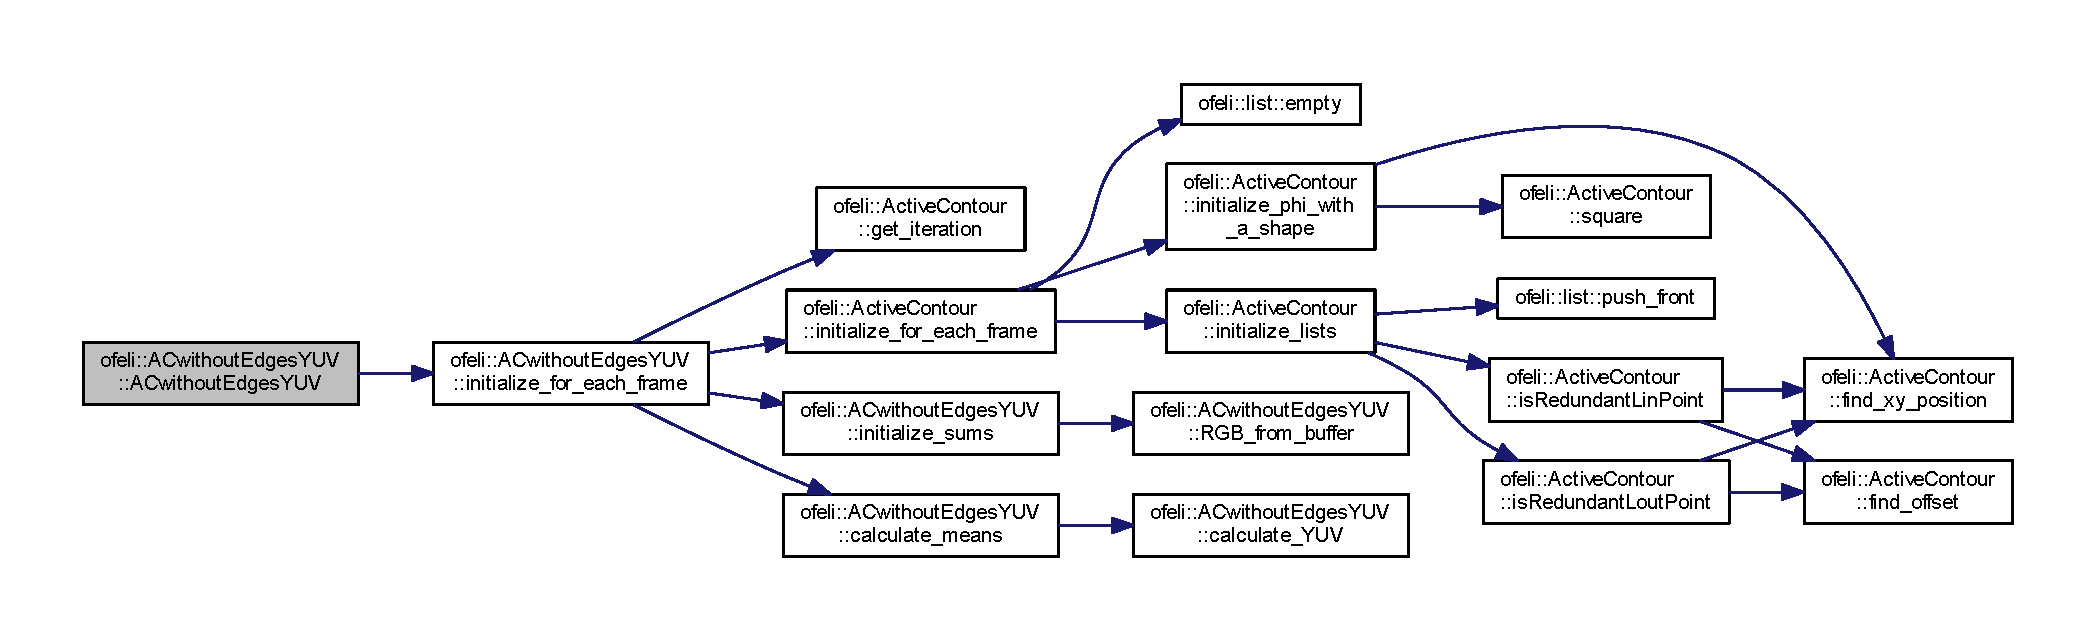
\includegraphics[width=350pt]{classofeli_1_1_a_cwithout_edges_y_u_v_a31765b6ebe4825cc2a1ea815d1235c22_cgraph}
\end{center}
\end{figure}


\hypertarget{classofeli_1_1_a_cwithout_edges_y_u_v_a63c5bcb0da045d930be9be686c5f5245}{\index{ofeli\-::\-A\-Cwithout\-Edges\-Y\-U\-V@{ofeli\-::\-A\-Cwithout\-Edges\-Y\-U\-V}!A\-Cwithout\-Edges\-Y\-U\-V@{A\-Cwithout\-Edges\-Y\-U\-V}}
\index{A\-Cwithout\-Edges\-Y\-U\-V@{A\-Cwithout\-Edges\-Y\-U\-V}!ofeli::ACwithoutEdgesYUV@{ofeli\-::\-A\-Cwithout\-Edges\-Y\-U\-V}}
\subsubsection[{A\-Cwithout\-Edges\-Y\-U\-V}]{\setlength{\rightskip}{0pt plus 5cm}A\-Cwithout\-Edges\-Y\-U\-V\-::\-A\-Cwithout\-Edges\-Y\-U\-V (
\begin{DoxyParamCaption}
\item[{const unsigned char $\ast$}]{img\-\_\-rgb\-\_\-data1, }
\item[{int}]{img\-\_\-width1, }
\item[{int}]{img\-\_\-height1, }
\item[{const char $\ast$}]{phi\-\_\-init1, }
\item[{bool}]{has\-Cycle2\-\_\-1, }
\item[{int}]{kernel\-\_\-length1, }
\item[{double}]{sigma1, }
\item[{int}]{Na1, }
\item[{int}]{Ns1, }
\item[{int}]{lambda\-\_\-out1, }
\item[{int}]{lambda\-\_\-in1, }
\item[{int}]{alpha1, }
\item[{int}]{beta1, }
\item[{int}]{gamma1}
\end{DoxyParamCaption}
)}}\label{classofeli_1_1_a_cwithout_edges_y_u_v_a63c5bcb0da045d930be9be686c5f5245}


Constructor to initialize the active contour from an initial phi level-\/set function. 


\begin{DoxyParams}{Parameters}
{\em img\-\_\-rgb\-\_\-data1} & Input pointer on the R\-G\-B data image buffer. This buffer must be row-\/wise and interleaved (R1 G1 B1 R2 G2 B2 ...). Passed to \hyperlink{classofeli_1_1_active_contour_a96480d79e9a60817925903da233a5b1e}{img\-\_\-data}. \\
\hline
{\em img\-\_\-width1} & Image width, i.\-e. number of columns. Passed to \hyperlink{classofeli_1_1_active_contour_a3623de7ebc0d27ba7fac21a5929afbc6}{img\-\_\-width}. \\
\hline
{\em img\-\_\-height1} & Image height, i.\-e. number of rows. Passed to \hyperlink{classofeli_1_1_active_contour_a88d02b47bab737ec97fe3a7ea9554c0c}{img\-\_\-height}. \\
\hline
{\em phi\-\_\-init1} & Pointer on the initialized level-\/set function buffer. Copied to \hyperlink{classofeli_1_1_active_contour_aacb03a6ded4ca51cb52f58aeff955ef7}{phi}. \\
\hline
{\em has\-Cycle2\-\_\-1} & Boolean to have or not the curve smoothing, evolutions in the cycle 2 with an internal speed {\itshape Fint}. Passed to \hyperlink{classofeli_1_1_active_contour_aa763ff1bed211faa444013cbd5de0be3}{has\-Cycle2}. \\
\hline
{\em kernel\-\_\-length1} & Kernel length of the gaussian filter for the curve smoothing. Passed to \hyperlink{classofeli_1_1_active_contour_a2b32161d0a9ac64a4e4f4c242fabe27c}{kernel\-\_\-length}. \\
\hline
{\em sigma1} & Standard deviation of the gaussian kernel for the curve smoothing. Passed to \hyperlink{classofeli_1_1_active_contour_a66303b7f6b88270133462feb303b039a}{sigma}. \\
\hline
{\em Na1} & Number of times the active contour evolves in the cycle 1, external or data dependant evolutions with {\itshape Fd} speed. Passed to \hyperlink{classofeli_1_1_active_contour_a811a28ec9c39400d244783a8a2fe7e2d}{Na\-\_\-max}. \\
\hline
{\em Ns1} & Number of times the active contour evolves in the cycle 2, curve smoothing or internal evolutions with {\itshape Fint} speed. Passed to \hyperlink{classofeli_1_1_active_contour_a908322f93a50ce7808960236478649fe}{Ns\-\_\-max}. \\
\hline
{\em lambda\-\_\-out1} & Weight of the outside homogeneity criterion. Passed to \hyperlink{classofeli_1_1_a_cwithout_edges_y_u_v_a7e638b979761b49ad1aecc50a194dad0}{lambda\-\_\-out}. \\
\hline
{\em lambda\-\_\-in1} & Weight of the inside homogeneity criterion. Passed to \hyperlink{classofeli_1_1_a_cwithout_edges_y_u_v_a311f8c97d1fbdcdbb76b1b09aea59212}{lambda\-\_\-in}. \\
\hline
{\em alpha1} & Weight of luminance Y. Passed to \hyperlink{classofeli_1_1_a_cwithout_edges_y_u_v_a613340fb017ff19af8510c9d72c9663b}{alpha}. \\
\hline
{\em beta1} & Weight of chrominance U. Passed to \hyperlink{classofeli_1_1_a_cwithout_edges_y_u_v_ae341898fb9f83bf41a731e1ada24cf0a}{beta}. \\
\hline
{\em gamma1} & Weight of chrominance V. Passed to \hyperlink{classofeli_1_1_a_cwithout_edges_y_u_v_a249bf1ba21819ddb9f63f0ceef8a97b2}{gamma}. \\
\hline
\end{DoxyParams}


Definition at line 74 of file ac\-\_\-withoutedges\-\_\-yuv.\-cpp.



Here is the call graph for this function\-:\nopagebreak
\begin{figure}[H]
\begin{center}
\leavevmode
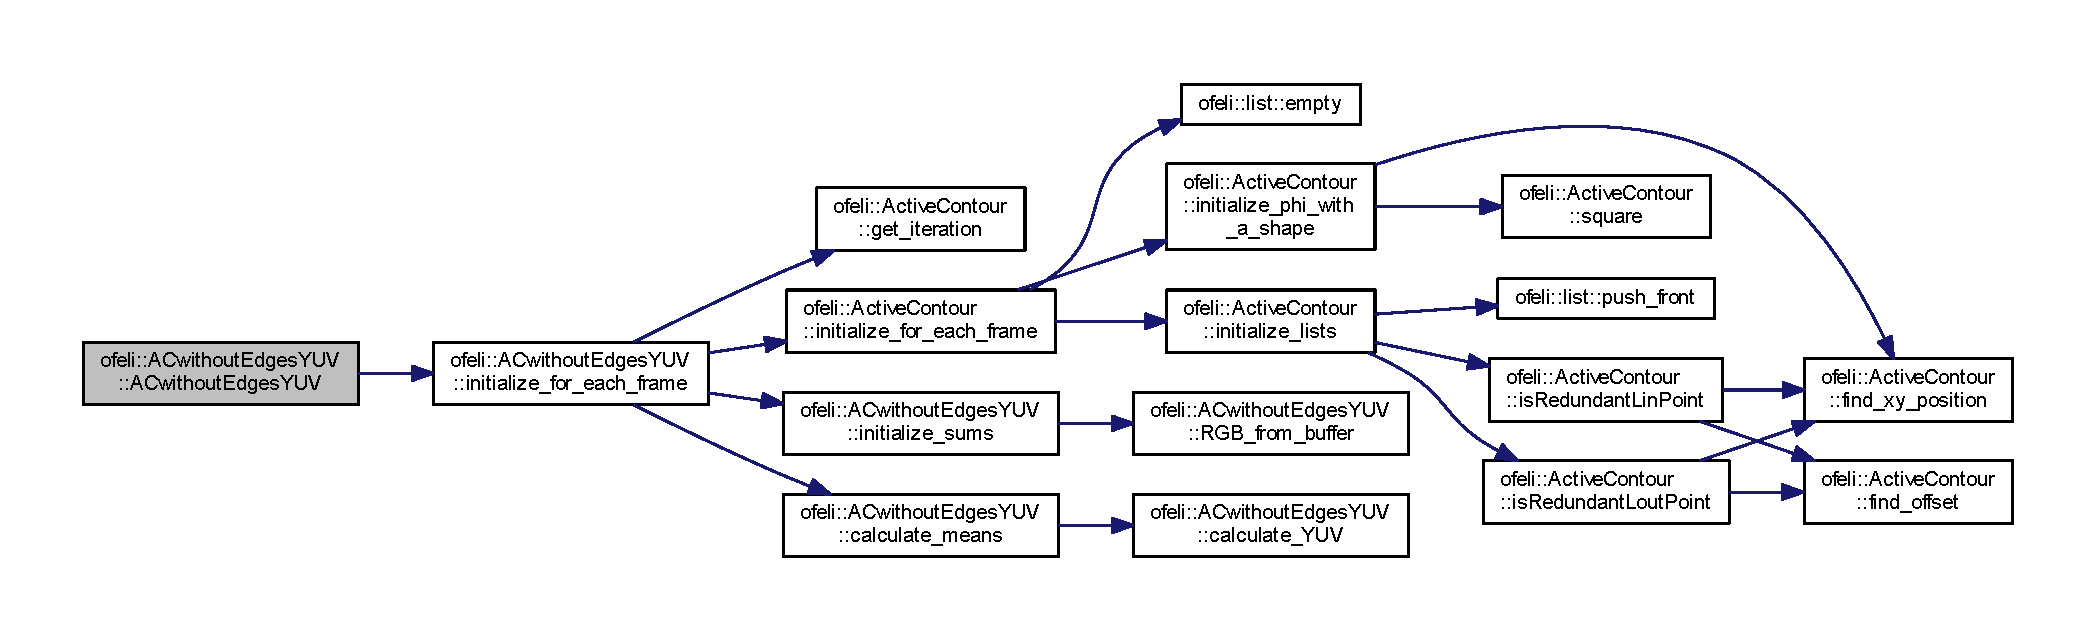
\includegraphics[width=350pt]{classofeli_1_1_a_cwithout_edges_y_u_v_a63c5bcb0da045d930be9be686c5f5245_cgraph}
\end{center}
\end{figure}




\subsection{Member Function Documentation}
\hypertarget{classofeli_1_1_a_cwithout_edges_y_u_v_ae61e98ace069646a009de7cd7148e065}{\index{ofeli\-::\-A\-Cwithout\-Edges\-Y\-U\-V@{ofeli\-::\-A\-Cwithout\-Edges\-Y\-U\-V}!compute\-\_\-external\-\_\-speed\-\_\-\-Fd@{compute\-\_\-external\-\_\-speed\-\_\-\-Fd}}
\index{compute\-\_\-external\-\_\-speed\-\_\-\-Fd@{compute\-\_\-external\-\_\-speed\-\_\-\-Fd}!ofeli::ACwithoutEdgesYUV@{ofeli\-::\-A\-Cwithout\-Edges\-Y\-U\-V}}
\subsubsection[{compute\-\_\-external\-\_\-speed\-\_\-\-Fd}]{\setlength{\rightskip}{0pt plus 5cm}void A\-Cwithout\-Edges\-Y\-U\-V\-::compute\-\_\-external\-\_\-speed\-\_\-\-Fd (
\begin{DoxyParamCaption}
\item[{int}]{offset}
\end{DoxyParamCaption}
)\hspace{0.3cm}{\ttfamily [private]}, {\ttfamily [virtual]}}}\label{classofeli_1_1_a_cwithout_edges_y_u_v_ae61e98ace069646a009de7cd7148e065}


Computes external speed {\itshape Fd} with the Chan-\/\-Vese model for a current point {\itshape }(x,y) of \hyperlink{classofeli_1_1_active_contour_a31e0eb18a7ea6ae90acf66ed018fcd85}{Lout} or \hyperlink{classofeli_1_1_active_contour_a7662d4f5c8b87d3e642b08b7e341bd79}{Lin}. 


\begin{DoxyParams}{Parameters}
{\em offset} & offset of the image data buffer with {\itshape offset} = {\itshape x} + {\itshape y} × \hyperlink{classofeli_1_1_active_contour_a3623de7ebc0d27ba7fac21a5929afbc6}{img\-\_\-width} \\
\hline
\end{DoxyParams}


Reimplemented from \hyperlink{classofeli_1_1_active_contour_ae3871b40f2f3e27ae0d75775798cdee1}{ofeli\-::\-Active\-Contour}.



Definition at line 187 of file ac\-\_\-withoutedges\-\_\-yuv.\-cpp.



Here is the call graph for this function\-:\nopagebreak
\begin{figure}[H]
\begin{center}
\leavevmode
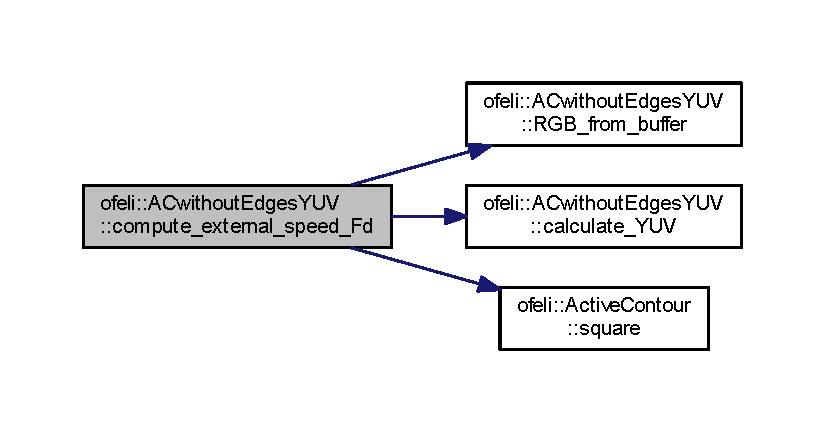
\includegraphics[width=350pt]{classofeli_1_1_a_cwithout_edges_y_u_v_ae61e98ace069646a009de7cd7148e065_cgraph}
\end{center}
\end{figure}


\hypertarget{classofeli_1_1_a_cwithout_edges_y_u_v_a249aa0e9664cf4f024997ac4475fe70c}{\index{ofeli\-::\-A\-Cwithout\-Edges\-Y\-U\-V@{ofeli\-::\-A\-Cwithout\-Edges\-Y\-U\-V}!updates\-\_\-for\-\_\-means\-\_\-in2@{updates\-\_\-for\-\_\-means\-\_\-in2}}
\index{updates\-\_\-for\-\_\-means\-\_\-in2@{updates\-\_\-for\-\_\-means\-\_\-in2}!ofeli::ACwithoutEdgesYUV@{ofeli\-::\-A\-Cwithout\-Edges\-Y\-U\-V}}
\subsubsection[{updates\-\_\-for\-\_\-means\-\_\-in2}]{\setlength{\rightskip}{0pt plus 5cm}void A\-Cwithout\-Edges\-Y\-U\-V\-::updates\-\_\-for\-\_\-means\-\_\-in2 (
\begin{DoxyParamCaption}
\item[{int}]{offset}
\end{DoxyParamCaption}
)\hspace{0.3cm}{\ttfamily [private]}, {\ttfamily [virtual]}}}\label{classofeli_1_1_a_cwithout_edges_y_u_v_a249aa0e9664cf4f024997ac4475fe70c}


Updates the six sums, \hyperlink{classofeli_1_1_a_cwithout_edges_y_u_v_a63542bb13e9dd879714b6c71cd5fe62c}{n\-\_\-in} and \hyperlink{classofeli_1_1_a_cwithout_edges_y_u_v_a034adbc67a268bd84539fe8e76b9deec}{n\-\_\-out}, before each \hyperlink{classofeli_1_1_active_contour_a7d9a557b580af708155ff4ab8bbfd73b}{switch\-\_\-in}, in the cycle 2, in order to calculate means \hyperlink{classofeli_1_1_a_cwithout_edges_y_u_v_a1aea515bf36ea9f426cc653802252ce5}{Cout\-Y\-U\-V} and \hyperlink{classofeli_1_1_a_cwithout_edges_y_u_v_ac5976def2629d484df763de752bb165d}{Cin\-Y\-U\-V}. 


\begin{DoxyParams}{Parameters}
{\em offset} & offset of the image data buffer with {\itshape offset} = {\itshape x} + {\itshape y} × \hyperlink{classofeli_1_1_active_contour_a3623de7ebc0d27ba7fac21a5929afbc6}{img\-\_\-width} \\
\hline
\end{DoxyParams}


Reimplemented from \hyperlink{classofeli_1_1_active_contour_a77e9dc7bcbd0ba48499a499891e021cb}{ofeli\-::\-Active\-Contour}.



Definition at line 233 of file ac\-\_\-withoutedges\-\_\-yuv.\-cpp.



Here is the call graph for this function\-:\nopagebreak
\begin{figure}[H]
\begin{center}
\leavevmode
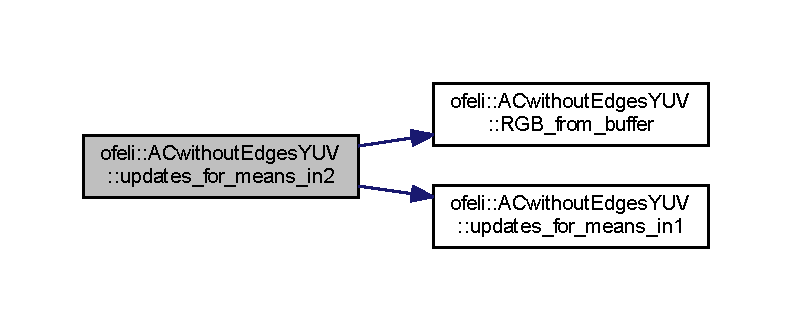
\includegraphics[width=350pt]{classofeli_1_1_a_cwithout_edges_y_u_v_a249aa0e9664cf4f024997ac4475fe70c_cgraph}
\end{center}
\end{figure}


\hypertarget{classofeli_1_1_a_cwithout_edges_y_u_v_a43b463f3b8d5cb9604fd73b18083409a}{\index{ofeli\-::\-A\-Cwithout\-Edges\-Y\-U\-V@{ofeli\-::\-A\-Cwithout\-Edges\-Y\-U\-V}!updates\-\_\-for\-\_\-means\-\_\-out2@{updates\-\_\-for\-\_\-means\-\_\-out2}}
\index{updates\-\_\-for\-\_\-means\-\_\-out2@{updates\-\_\-for\-\_\-means\-\_\-out2}!ofeli::ACwithoutEdgesYUV@{ofeli\-::\-A\-Cwithout\-Edges\-Y\-U\-V}}
\subsubsection[{updates\-\_\-for\-\_\-means\-\_\-out2}]{\setlength{\rightskip}{0pt plus 5cm}A\-Cwithout\-Edges\-Y\-U\-V\-::updates\-\_\-for\-\_\-means\-\_\-out2 (
\begin{DoxyParamCaption}
\item[{int}]{offset}
\end{DoxyParamCaption}
)\hspace{0.3cm}{\ttfamily [private]}, {\ttfamily [virtual]}}}\label{classofeli_1_1_a_cwithout_edges_y_u_v_a43b463f3b8d5cb9604fd73b18083409a}


Updates the six sums, \hyperlink{classofeli_1_1_a_cwithout_edges_y_u_v_a63542bb13e9dd879714b6c71cd5fe62c}{n\-\_\-in} and \hyperlink{classofeli_1_1_a_cwithout_edges_y_u_v_a034adbc67a268bd84539fe8e76b9deec}{n\-\_\-out}, before each \hyperlink{classofeli_1_1_active_contour_a98af656dfc038e6f03c9e4bb67e39bd0}{switch\-\_\-out}, in the cycle 2, in order to calculate means \hyperlink{classofeli_1_1_a_cwithout_edges_y_u_v_a1aea515bf36ea9f426cc653802252ce5}{Cout\-Y\-U\-V} and \hyperlink{classofeli_1_1_a_cwithout_edges_y_u_v_ac5976def2629d484df763de752bb165d}{Cin\-Y\-U\-V}. 


\begin{DoxyParams}{Parameters}
{\em offset} & offset of the image data buffer with {\itshape offset} = {\itshape x} + {\itshape y} × \hyperlink{classofeli_1_1_active_contour_a3623de7ebc0d27ba7fac21a5929afbc6}{img\-\_\-width} \\
\hline
\end{DoxyParams}


Reimplemented from \hyperlink{classofeli_1_1_active_contour_a347e650493750ad29b8b73ed52bdcf7a}{ofeli\-::\-Active\-Contour}.



Definition at line 242 of file ac\-\_\-withoutedges\-\_\-yuv.\-cpp.



Here is the call graph for this function\-:\nopagebreak
\begin{figure}[H]
\begin{center}
\leavevmode
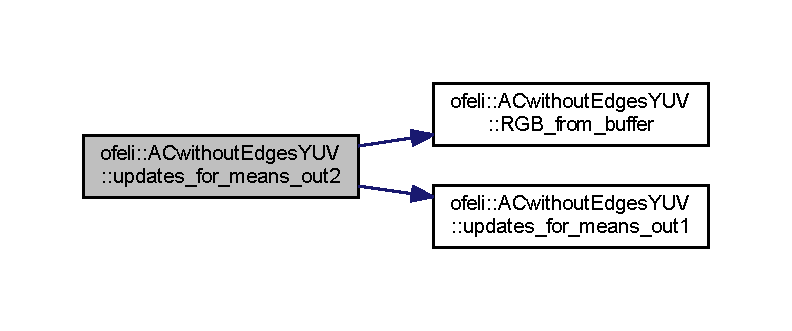
\includegraphics[width=350pt]{classofeli_1_1_a_cwithout_edges_y_u_v_a43b463f3b8d5cb9604fd73b18083409a_cgraph}
\end{center}
\end{figure}




The documentation for this class was generated from the following files\-:\begin{DoxyCompactItemize}
\item 
ac\-\_\-withoutedges\-\_\-yuv.\-hpp\item 
ac\-\_\-withoutedges\-\_\-yuv.\-cpp\end{DoxyCompactItemize}

\hypertarget{classofeli_1_1list_1_1const__iterator}{\section{ofeli\-:\-:list$<$ T $>$\-:\-:const\-\_\-iterator Class Reference}
\label{classofeli_1_1list_1_1const__iterator}\index{ofeli\-::list$<$ T $>$\-::const\-\_\-iterator@{ofeli\-::list$<$ T $>$\-::const\-\_\-iterator}}
}


const iterator to read a const list.  




{\ttfamily \#include $<$linked\-\_\-list.\-hpp$>$}



Collaboration diagram for ofeli\-:\-:list$<$ T $>$\-:\-:const\-\_\-iterator\-:\nopagebreak
\begin{figure}[H]
\begin{center}
\leavevmode
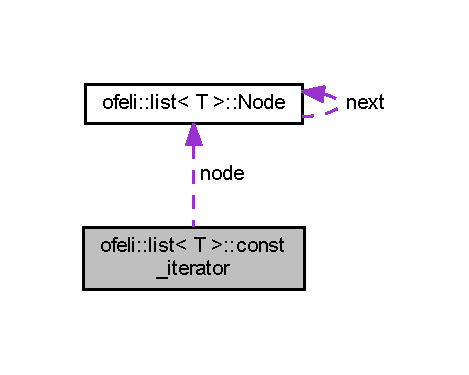
\includegraphics[width=225pt]{classofeli_1_1list_1_1const__iterator__coll__graph}
\end{center}
\end{figure}
\subsection*{Public Member Functions}
\begin{DoxyCompactItemize}
\item 
\hypertarget{classofeli_1_1list_1_1const__iterator_a2d0a1de571a02588a0dee230dc1534d2}{const T \& \hyperlink{classofeli_1_1list_1_1const__iterator_a2d0a1de571a02588a0dee230dc1534d2}{operator$\ast$} () const }\label{classofeli_1_1list_1_1const__iterator_a2d0a1de571a02588a0dee230dc1534d2}

\begin{DoxyCompactList}\small\item\em Gets the node data. {\itshape \hyperlink{classofeli_1_1list_1_1const__iterator}{const\-\_\-iterator}} protects the data against writing. \end{DoxyCompactList}\item 
\hypertarget{classofeli_1_1list_1_1const__iterator_aa79779e28253e61c8d1816f577de4ffd}{bool \hyperlink{classofeli_1_1list_1_1const__iterator_aa79779e28253e61c8d1816f577de4ffd}{end} () const }\label{classofeli_1_1list_1_1const__iterator_aa79779e28253e61c8d1816f577de4ffd}

\begin{DoxyCompactList}\small\item\em Checks if the {\itshape \hyperlink{classofeli_1_1list_1_1const__iterator}{const\-\_\-iterator}} is at the end of the list, i.\-e. if the node is the sentinel node. \end{DoxyCompactList}\item 
\hypertarget{classofeli_1_1list_1_1const__iterator_a31e40395e411104489e4235b775869ec}{\hyperlink{classofeli_1_1list_1_1const__iterator}{const\-\_\-iterator} \& \hyperlink{classofeli_1_1list_1_1const__iterator_a31e40395e411104489e4235b775869ec}{operator++} ()}\label{classofeli_1_1list_1_1const__iterator_a31e40395e411104489e4235b775869ec}

\begin{DoxyCompactList}\small\item\em Increment {\itshape \hyperlink{classofeli_1_1list_1_1const__iterator}{const\-\_\-iterator}}. \end{DoxyCompactList}\end{DoxyCompactItemize}
\subsection*{Private Member Functions}
\begin{DoxyCompactItemize}
\item 
\hypertarget{classofeli_1_1list_1_1const__iterator_a42996141faaf25e061ecf726a66c141b}{\hyperlink{classofeli_1_1list_1_1const__iterator_a42996141faaf25e061ecf726a66c141b}{const\-\_\-iterator} (\hyperlink{classofeli_1_1list_a7765ecb875543506d04dbd466f754503}{Link} node1)}\label{classofeli_1_1list_1_1const__iterator_a42996141faaf25e061ecf726a66c141b}

\begin{DoxyCompactList}\small\item\em Constructor with a node. \end{DoxyCompactList}\end{DoxyCompactItemize}
\subsection*{Private Attributes}
\begin{DoxyCompactItemize}
\item 
\hypertarget{classofeli_1_1list_1_1const__iterator_a4d13eb002aeaaa460605719cd043d116}{\hyperlink{classofeli_1_1list_a7765ecb875543506d04dbd466f754503}{Link} \hyperlink{classofeli_1_1list_1_1const__iterator_a4d13eb002aeaaa460605719cd043d116}{node}}\label{classofeli_1_1list_1_1const__iterator_a4d13eb002aeaaa460605719cd043d116}

\begin{DoxyCompactList}\small\item\em {\itshape \hyperlink{classofeli_1_1list_1_1const__iterator}{const\-\_\-iterator}} encapsulates a pointer to a node. \end{DoxyCompactList}\end{DoxyCompactItemize}
\subsection*{Friends}
\begin{DoxyCompactItemize}
\item 
\hypertarget{classofeli_1_1list_1_1const__iterator_a39e8296e3b93358d0af90000b5d9113c}{class \hyperlink{classofeli_1_1list_1_1const__iterator_a39e8296e3b93358d0af90000b5d9113c}{list}}\label{classofeli_1_1list_1_1const__iterator_a39e8296e3b93358d0af90000b5d9113c}

\begin{DoxyCompactList}\small\item\em list has access to the private members of {\itshape \hyperlink{classofeli_1_1list_1_1const__iterator}{const\-\_\-iterator}}. \end{DoxyCompactList}\end{DoxyCompactItemize}


\subsection{Detailed Description}
\subsubsection*{template$<$typename T = int$>$class ofeli\-::list$<$ T $>$\-::const\-\_\-iterator}

const iterator to read a const list. \begin{Desc}
\item[Examples\-: ]\par
\hyperlink{interface-example}{interface}, and \hyperlink{linked_list-example}{linked\-\_\-list}.\end{Desc}


Definition at line 80 of file linked\-\_\-list.\-hpp.



The documentation for this class was generated from the following file\-:\begin{DoxyCompactItemize}
\item 
linked\-\_\-list.\-hpp\end{DoxyCompactItemize}

\hypertarget{structofeli_1_1equal__to}{\section{ofeli\-:\-:equal\-\_\-to$<$ T $>$ Struct Template Reference}
\label{structofeli_1_1equal__to}\index{ofeli\-::equal\-\_\-to$<$ T $>$@{ofeli\-::equal\-\_\-to$<$ T $>$}}
}


{\ttfamily \#include $<$linked\-\_\-list.\-hpp$>$}

\subsection*{Public Member Functions}
\begin{DoxyCompactItemize}
\item 
\hypertarget{structofeli_1_1equal__to_a27b12a625a6eb0955bc710c57882d24c}{bool {\bfseries operator()} (const T \&x, const T \&y) const }\label{structofeli_1_1equal__to_a27b12a625a6eb0955bc710c57882d24c}

\end{DoxyCompactItemize}


\subsection{Detailed Description}
\subsubsection*{template$<$typename T = int$>$struct ofeli\-::equal\-\_\-to$<$ T $>$}

This class defines function objects for the equality comparison operation. Generically, function objects are instances of a class with member function {\ttfamily operator()} defined. This member function allows the object to be used with the same syntax as a regular function call, and therefore it can be used in templates instead of a pointer to a function. {\ttfamily \hyperlink{structofeli_1_1equal__to}{equal\-\_\-to}} has its {\ttfamily operator()} member defined such that it returns {\ttfamily true} if its two arguments compare equal to each other using {\ttfamily operator==}, and {\ttfamily false} otherwise. This class can be used with the template functions {\ttfamily \hyperlink{classofeli_1_1list_aaeedac18b70d233644d84c7ad3a9a3fa}{list$<$\-T$>$\-::sort(\-Binary\-Predicate compare)}} and list$<$\-T$>$\-::put\-\_\-away(\-Binary\-Predicate compare). 

Definition at line 376 of file linked\-\_\-list.\-hpp.



The documentation for this struct was generated from the following file\-:\begin{DoxyCompactItemize}
\item 
linked\-\_\-list.\-hpp\end{DoxyCompactItemize}

\hypertarget{classofeli_1_1_filters}{\section{ofeli\-:\-:Filters Class Reference}
\label{classofeli_1_1_filters}\index{ofeli\-::\-Filters@{ofeli\-::\-Filters}}
}


{\ttfamily \#include $<$filters.\-hpp$>$}

\subsection*{Public Member Functions}
\begin{DoxyCompactItemize}
\item 
\hypertarget{classofeli_1_1_filters_afdfd38460d9612c305776f4488a14546}{\hyperlink{classofeli_1_1_filters_afdfd38460d9612c305776f4488a14546}{Filters} (const unsigned char $\ast$img\-\_\-data1, int img\-\_\-width1, int img\-\_\-height1, int byte\-\_\-per\-\_\-pixel1)}\label{classofeli_1_1_filters_afdfd38460d9612c305776f4488a14546}

\begin{DoxyCompactList}\small\item\em Constructor with an input pointer on a row-\/wise image data buffer and the dimensions of the image. \end{DoxyCompactList}\item 
\hypertarget{classofeli_1_1_filters_aca1ba583de5930e46a3df2110ebbf21c}{\hyperlink{classofeli_1_1_filters_aca1ba583de5930e46a3df2110ebbf21c}{$\sim$\-Filters} ()}\label{classofeli_1_1_filters_aca1ba583de5930e46a3df2110ebbf21c}

\begin{DoxyCompactList}\small\item\em Desctructor. \end{DoxyCompactList}\item 
\hypertarget{classofeli_1_1_filters_a4bd1f0541cb045674548e292180fff0f}{void \hyperlink{classofeli_1_1_filters_a4bd1f0541cb045674548e292180fff0f}{initialyze\-\_\-filtered} ()}\label{classofeli_1_1_filters_a4bd1f0541cb045674548e292180fff0f}

\begin{DoxyCompactList}\small\item\em Copies {\itshape img} buffer to {\itshape filtered} buffer. \end{DoxyCompactList}\item 
void \hyperlink{classofeli_1_1_filters_ae4a65a5259b3a91a523eefdf2d90b920}{anisotropic\-\_\-diffusion} (int max\-\_\-itera, double lambda, double kappa, int option)
\begin{DoxyCompactList}\small\item\em Performs a Perona-\/\-Malik anisotropic diffusion with a 8-\/connected neighborhood. \end{DoxyCompactList}\item 
\hypertarget{classofeli_1_1_filters_a95fcd4385d6a115af0617407d91e6901}{void \hyperlink{classofeli_1_1_filters_a95fcd4385d6a115af0617407d91e6901}{morphological\-\_\-gradient} (int kernel\-\_\-length)}\label{classofeli_1_1_filters_a95fcd4385d6a115af0617407d91e6901}

\begin{DoxyCompactList}\small\item\em Performs a morphological\-\_\-gradient with a square structuring element with a naïve algorithm. \end{DoxyCompactList}\item 
\hypertarget{classofeli_1_1_filters_a13b390c3705e19c211c04f47daa17844}{void \hyperlink{classofeli_1_1_filters_a13b390c3705e19c211c04f47daa17844}{morphological\-\_\-gradient\-\_\-o1} (int kernel\-\_\-length)}\label{classofeli_1_1_filters_a13b390c3705e19c211c04f47daa17844}

\begin{DoxyCompactList}\small\item\em Performs a morphological\-\_\-gradient with a square structuring element with the Perreault's algorithm. \end{DoxyCompactList}\item 
\hypertarget{classofeli_1_1_filters_aceefc0f308d675d2cb752bd4a7a22dd1}{void \hyperlink{classofeli_1_1_filters_aceefc0f308d675d2cb752bd4a7a22dd1}{dilation} (int kernel\-\_\-length)}\label{classofeli_1_1_filters_aceefc0f308d675d2cb752bd4a7a22dd1}

\begin{DoxyCompactList}\small\item\em Performs a dilation with a square structuring element with a naïve algorithm. \end{DoxyCompactList}\item 
\hypertarget{classofeli_1_1_filters_a806b4e3976167324fa019d825e00286d}{void \hyperlink{classofeli_1_1_filters_a806b4e3976167324fa019d825e00286d}{dilation\-\_\-o1} (int kernel\-\_\-length)}\label{classofeli_1_1_filters_a806b4e3976167324fa019d825e00286d}

\begin{DoxyCompactList}\small\item\em Performs a dilation with a square structuring element with the Perreault's algorithm. \end{DoxyCompactList}\item 
\hypertarget{classofeli_1_1_filters_ab9bc3d5a53898251178515d5d6be8293}{void \hyperlink{classofeli_1_1_filters_ab9bc3d5a53898251178515d5d6be8293}{erosion} (int kernel\-\_\-length)}\label{classofeli_1_1_filters_ab9bc3d5a53898251178515d5d6be8293}

\begin{DoxyCompactList}\small\item\em Performs an erosion with a square structuring element with a naïve algorithm. \end{DoxyCompactList}\item 
\hypertarget{classofeli_1_1_filters_a8f6d16a2ebbc52ea041cda0c7336343a}{void \hyperlink{classofeli_1_1_filters_a8f6d16a2ebbc52ea041cda0c7336343a}{erosion\-\_\-o1} (int kernel\-\_\-length)}\label{classofeli_1_1_filters_a8f6d16a2ebbc52ea041cda0c7336343a}

\begin{DoxyCompactList}\small\item\em Performs an erosion with a square structuring element with the Perreault's algorithm. \end{DoxyCompactList}\item 
\hypertarget{classofeli_1_1_filters_a01cbcf40deec00feca16f982e3e081a2}{void \hyperlink{classofeli_1_1_filters_a01cbcf40deec00feca16f982e3e081a2}{closing} (int kernel\-\_\-length)}\label{classofeli_1_1_filters_a01cbcf40deec00feca16f982e3e081a2}

\begin{DoxyCompactList}\small\item\em Performs a closing with a square structuring element with a naïve algorithm. \end{DoxyCompactList}\item 
\hypertarget{classofeli_1_1_filters_a04f01e51d6feee4246ede96f767d36c5}{void \hyperlink{classofeli_1_1_filters_a04f01e51d6feee4246ede96f767d36c5}{closing\-\_\-o1} (int kernel\-\_\-length)}\label{classofeli_1_1_filters_a04f01e51d6feee4246ede96f767d36c5}

\begin{DoxyCompactList}\small\item\em Performs a closing with a square structuring element with the Perreault's algorithm. \end{DoxyCompactList}\item 
\hypertarget{classofeli_1_1_filters_aab4788b300a3229c61b7cae344eb2142}{void \hyperlink{classofeli_1_1_filters_aab4788b300a3229c61b7cae344eb2142}{opening} (int kernel\-\_\-length)}\label{classofeli_1_1_filters_aab4788b300a3229c61b7cae344eb2142}

\begin{DoxyCompactList}\small\item\em Performs a closing with a square structuring element with a naïve algorithm. \end{DoxyCompactList}\item 
\hypertarget{classofeli_1_1_filters_a157720e1dbc58827f515de30a18b546a}{void \hyperlink{classofeli_1_1_filters_a157720e1dbc58827f515de30a18b546a}{opening\-\_\-o1} (int kernel\-\_\-length)}\label{classofeli_1_1_filters_a157720e1dbc58827f515de30a18b546a}

\begin{DoxyCompactList}\small\item\em Performs an opening with a square structuring element with the Perreault's algorithm. \end{DoxyCompactList}\item 
\hypertarget{classofeli_1_1_filters_a29dbdd34e2cffc4f37b104f3fab6ead0}{void \hyperlink{classofeli_1_1_filters_a29dbdd34e2cffc4f37b104f3fab6ead0}{black\-\_\-top\-\_\-hat} (int kernel\-\_\-length)}\label{classofeli_1_1_filters_a29dbdd34e2cffc4f37b104f3fab6ead0}

\begin{DoxyCompactList}\small\item\em Performs a black top hat transform with a square structuring element with a naïve algorithm. \end{DoxyCompactList}\item 
\hypertarget{classofeli_1_1_filters_a6343e4176fd069a285b6da83de0cd63d}{void \hyperlink{classofeli_1_1_filters_a6343e4176fd069a285b6da83de0cd63d}{black\-\_\-top\-\_\-hat\-\_\-o1} (int kernel\-\_\-length)}\label{classofeli_1_1_filters_a6343e4176fd069a285b6da83de0cd63d}

\begin{DoxyCompactList}\small\item\em Performs a black top hat transform with a square structuring element with the Perreault's algorithm. \end{DoxyCompactList}\item 
\hypertarget{classofeli_1_1_filters_adaade4352062899127d46615a8e31b42}{void \hyperlink{classofeli_1_1_filters_adaade4352062899127d46615a8e31b42}{white\-\_\-top\-\_\-hat} (int kernel\-\_\-length)}\label{classofeli_1_1_filters_adaade4352062899127d46615a8e31b42}

\begin{DoxyCompactList}\small\item\em Performs a white top hat transform with a square structuring element with a naïve algorithm. \end{DoxyCompactList}\item 
\hypertarget{classofeli_1_1_filters_a2e3a6b4aa3329dcb021430748c83d992}{void \hyperlink{classofeli_1_1_filters_a2e3a6b4aa3329dcb021430748c83d992}{white\-\_\-top\-\_\-hat\-\_\-o1} (int kernel\-\_\-length)}\label{classofeli_1_1_filters_a2e3a6b4aa3329dcb021430748c83d992}

\begin{DoxyCompactList}\small\item\em Performs a white top hat transform with a square structuring element with the Perreault's algorithm. \end{DoxyCompactList}\item 
\hypertarget{classofeli_1_1_filters_a525926351892d87d4fee244474d9ac8f}{void \hyperlink{classofeli_1_1_filters_a525926351892d87d4fee244474d9ac8f}{fas} (int kernel\-\_\-length)}\label{classofeli_1_1_filters_a525926351892d87d4fee244474d9ac8f}

\begin{DoxyCompactList}\small\item\em Performs a filter alternate sequential. \end{DoxyCompactList}\item 
\hypertarget{classofeli_1_1_filters_a9b4e4ebbfe46d648181eb4193d829972}{void \hyperlink{classofeli_1_1_filters_a9b4e4ebbfe46d648181eb4193d829972}{mean\-\_\-filtering} (int kernel\-\_\-length)}\label{classofeli_1_1_filters_a9b4e4ebbfe46d648181eb4193d829972}

\begin{DoxyCompactList}\small\item\em Performs a mean filtering. \end{DoxyCompactList}\item 
\hypertarget{classofeli_1_1_filters_ac34d1b5157e16d92176acc0548f62ff3}{void \hyperlink{classofeli_1_1_filters_ac34d1b5157e16d92176acc0548f62ff3}{nagao\-\_\-filtering} (int kernel\-\_\-length)}\label{classofeli_1_1_filters_ac34d1b5157e16d92176acc0548f62ff3}

\begin{DoxyCompactList}\small\item\em Performs a Nagao filtering. \end{DoxyCompactList}\item 
\hypertarget{classofeli_1_1_filters_a22c697b23c38bc3122975e3b923d2bf2}{void \hyperlink{classofeli_1_1_filters_a22c697b23c38bc3122975e3b923d2bf2}{gaussian\-\_\-filtering} (int kernel\-\_\-length, double sigma)}\label{classofeli_1_1_filters_a22c697b23c38bc3122975e3b923d2bf2}

\begin{DoxyCompactList}\small\item\em Performs a gaussian filtering with the kernel length and the standard deviation {\ttfamily sigma}. \end{DoxyCompactList}\item 
\hypertarget{classofeli_1_1_filters_a2dff0282c738fff489f18d9173cfec24}{void \hyperlink{classofeli_1_1_filters_a2dff0282c738fff489f18d9173cfec24}{median\-\_\-filtering\-\_\-o\-Nlog\-N} (int kernel\-\_\-length)}\label{classofeli_1_1_filters_a2dff0282c738fff489f18d9173cfec24}

\begin{DoxyCompactList}\small\item\em Performs a median filtering based on the quick sort algorithm. Complexity is in {\ttfamily O}(kernel\-\_\-length×log(kernel\-\_\-length)). \end{DoxyCompactList}\item 
\hypertarget{classofeli_1_1_filters_a65e7324360cac62a715a61565399ad85}{void \hyperlink{classofeli_1_1_filters_a65e7324360cac62a715a61565399ad85}{median\-\_\-filtering\-\_\-o1} (int kernel\-\_\-length)}\label{classofeli_1_1_filters_a65e7324360cac62a715a61565399ad85}

\begin{DoxyCompactList}\small\item\em Performs a median filtering based on the Perreault's algorithm. Complexity is in {\ttfamily O(1)}. \end{DoxyCompactList}\item 
\hypertarget{classofeli_1_1_filters_a0351b099fb22a9397b27ae1661b6c836}{void \hyperlink{classofeli_1_1_filters_a0351b099fb22a9397b27ae1661b6c836}{gaussian\-\_\-white\-\_\-noise} (double sigma)}\label{classofeli_1_1_filters_a0351b099fb22a9397b27ae1661b6c836}

\begin{DoxyCompactList}\small\item\em Adds a gaussian white noise with the standard deviation {\ttfamily sigma}. \end{DoxyCompactList}\item 
\hypertarget{classofeli_1_1_filters_a268bff23cc4814805605782aaa9e7fa6}{void \hyperlink{classofeli_1_1_filters_a268bff23cc4814805605782aaa9e7fa6}{salt\-\_\-pepper\-\_\-noise} (double proba)}\label{classofeli_1_1_filters_a268bff23cc4814805605782aaa9e7fa6}

\begin{DoxyCompactList}\small\item\em Does an impulsional noise with a probabity of noise for each pixel, i.\-e the density. \end{DoxyCompactList}\item 
\hypertarget{classofeli_1_1_filters_a04349ff8309e50ed6daf714ff66f3239}{void \hyperlink{classofeli_1_1_filters_a04349ff8309e50ed6daf714ff66f3239}{speckle} (double sigma)}\label{classofeli_1_1_filters_a04349ff8309e50ed6daf714ff66f3239}

\begin{DoxyCompactList}\small\item\em Performs a speckle noise, a multiplicative noise into the image. \end{DoxyCompactList}\item 
\hypertarget{classofeli_1_1_filters_a0ef873a93af4eab1de166af4b500506b}{void \hyperlink{classofeli_1_1_filters_a0ef873a93af4eab1de166af4b500506b}{local\-\_\-binary\-\_\-pattern} (int kernel\-\_\-length)}\label{classofeli_1_1_filters_a0ef873a93af4eab1de166af4b500506b}

\begin{DoxyCompactList}\small\item\em Computes the local binary pattern. \end{DoxyCompactList}\item 
void \hyperlink{classofeli_1_1_filters_a0f29ec08c3d9febd2f95ba54ec88e524}{morphological\-\_\-gradient\-\_\-yuv} (int kernel\-\_\-length, int alpha, int beta, int gamma)
\begin{DoxyCompactList}\small\item\em Computes a morphological gradient \hyperlink{classofeli_1_1_filters_a9c02bc4005c55eeb5a426485af0d03a9}{gradient}. \end{DoxyCompactList}\item 
\hypertarget{classofeli_1_1_filters_a6ed876388f175010735b4987a1a6f493}{const unsigned char $\ast$ \hyperlink{classofeli_1_1_filters_a6ed876388f175010735b4987a1a6f493}{get\-\_\-filtered} () const }\label{classofeli_1_1_filters_a6ed876388f175010735b4987a1a6f493}

\begin{DoxyCompactList}\small\item\em Getter function for \hyperlink{classofeli_1_1_filters_aa4afdd919dfccb08023dee3634b03a30}{filtered}. \end{DoxyCompactList}\item 
\hypertarget{classofeli_1_1_filters_a2c2f355ff0267554a4b2257560fc0085}{const unsigned char $\ast$ \hyperlink{classofeli_1_1_filters_a2c2f355ff0267554a4b2257560fc0085}{get\-\_\-gradient} () const }\label{classofeli_1_1_filters_a2c2f355ff0267554a4b2257560fc0085}

\begin{DoxyCompactList}\small\item\em Getter function for \hyperlink{classofeli_1_1_filters_a9c02bc4005c55eeb5a426485af0d03a9}{gradient}. \end{DoxyCompactList}\end{DoxyCompactItemize}
\subsection*{Private Member Functions}
\begin{DoxyCompactItemize}
\item 
\hypertarget{classofeli_1_1_filters_ac7e55934e49bacdb8dffafa6d60eb948}{int \hyperlink{classofeli_1_1_filters_ac7e55934e49bacdb8dffafa6d60eb948}{find\-\_\-offset} (int x, int y, int color\-\_\-channel) const }\label{classofeli_1_1_filters_ac7e55934e49bacdb8dffafa6d60eb948}

\begin{DoxyCompactList}\small\item\em Calculates the offset the image data buffer with the position ({\itshape x},{\itshape y}, {\itshape color\-\_\-channel}). \end{DoxyCompactList}\end{DoxyCompactItemize}
\subsection*{Static Private Member Functions}
\begin{DoxyCompactItemize}
\item 
\hypertarget{classofeli_1_1_filters_abfd6b12417b42693a903e35f01608969}{static const double $\ast$const \hyperlink{classofeli_1_1_filters_abfd6b12417b42693a903e35f01608969}{gaussian\-\_\-kernel} (int kernel\-\_\-length, double sigma)}\label{classofeli_1_1_filters_abfd6b12417b42693a903e35f01608969}

\begin{DoxyCompactList}\small\item\em Creates a gaussian kernel with the kernel length and the standard deviation sigma. \end{DoxyCompactList}\item 
\hypertarget{classofeli_1_1_filters_afe930659890f200f2f8874ef68be5a10}{static void \hyperlink{classofeli_1_1_filters_afe930659890f200f2f8874ef68be5a10}{swap} (unsigned char $\ast$const array, int a, int b)}\label{classofeli_1_1_filters_afe930659890f200f2f8874ef68be5a10}

\begin{DoxyCompactList}\small\item\em Swaps two values of an array. \end{DoxyCompactList}\item 
\hypertarget{classofeli_1_1_filters_a93dda800c3f3a0053cccde23a457656f}{static void \hyperlink{classofeli_1_1_filters_a93dda800c3f3a0053cccde23a457656f}{quick\-\_\-sort} (unsigned char $\ast$const array, int begin, int end)}\label{classofeli_1_1_filters_a93dda800c3f3a0053cccde23a457656f}

\begin{DoxyCompactList}\small\item\em Sorts an array with the quick sort algorithm. \end{DoxyCompactList}\item 
\hypertarget{classofeli_1_1_filters_a4db66fc6e849d67e5bc89dbc72fe6282}{{\footnotesize template$<$typename T $>$ }\\static T \hyperlink{classofeli_1_1_filters_a4db66fc6e849d67e5bc89dbc72fe6282}{square} (const T \&value)}\label{classofeli_1_1_filters_a4db66fc6e849d67e5bc89dbc72fe6282}

\begin{DoxyCompactList}\small\item\em Gives the square of a value. \end{DoxyCompactList}\end{DoxyCompactItemize}
\subsection*{Private Attributes}
\begin{DoxyCompactItemize}
\item 
\hypertarget{classofeli_1_1_filters_a375494bcc04ceef4f48e859f2c8afe09}{const unsigned char $\ast$const \hyperlink{classofeli_1_1_filters_a375494bcc04ceef4f48e859f2c8afe09}{img\-\_\-data}}\label{classofeli_1_1_filters_a375494bcc04ceef4f48e859f2c8afe09}

\begin{DoxyCompactList}\small\item\em Input pointer on the grayscale or grey-\/level image data buffer. This buffer must be row-\/wise. \end{DoxyCompactList}\item 
\hypertarget{classofeli_1_1_filters_aa4afdd919dfccb08023dee3634b03a30}{unsigned char $\ast$ \hyperlink{classofeli_1_1_filters_aa4afdd919dfccb08023dee3634b03a30}{filtered}}\label{classofeli_1_1_filters_aa4afdd919dfccb08023dee3634b03a30}

\begin{DoxyCompactList}\small\item\em Pointer on the current result image. \end{DoxyCompactList}\item 
\hypertarget{classofeli_1_1_filters_adfafb4edd683c3cc02997328296df055}{const int \hyperlink{classofeli_1_1_filters_adfafb4edd683c3cc02997328296df055}{img\-\_\-width}}\label{classofeli_1_1_filters_adfafb4edd683c3cc02997328296df055}

\begin{DoxyCompactList}\small\item\em Image width, i.\-e. number of columns. \end{DoxyCompactList}\item 
\hypertarget{classofeli_1_1_filters_a433940423042a8efbdbf1576db1cfa70}{const int \hyperlink{classofeli_1_1_filters_a433940423042a8efbdbf1576db1cfa70}{img\-\_\-height}}\label{classofeli_1_1_filters_a433940423042a8efbdbf1576db1cfa70}

\begin{DoxyCompactList}\small\item\em Image height, i.\-e. number of rows. \end{DoxyCompactList}\item 
\hypertarget{classofeli_1_1_filters_a1c8ad08ed27f16f0def6416ff009599c}{const int \hyperlink{classofeli_1_1_filters_a1c8ad08ed27f16f0def6416ff009599c}{img\-\_\-size}}\label{classofeli_1_1_filters_a1c8ad08ed27f16f0def6416ff009599c}

\begin{DoxyCompactList}\small\item\em Image size, i.\-e. number of pixels. Obviously, it egals to \hyperlink{classofeli_1_1_filters_adfafb4edd683c3cc02997328296df055}{img\-\_\-width} × \hyperlink{classofeli_1_1_filters_a433940423042a8efbdbf1576db1cfa70}{img\-\_\-height}. \end{DoxyCompactList}\item 
\hypertarget{classofeli_1_1_filters_a229e0fc77f59c4747d0251e38cee38a9}{const int \hyperlink{classofeli_1_1_filters_a229e0fc77f59c4747d0251e38cee38a9}{byte\-\_\-per\-\_\-pixel}}\label{classofeli_1_1_filters_a229e0fc77f59c4747d0251e38cee38a9}

\begin{DoxyCompactList}\small\item\em Number of byte or octet per pixel, i.\-e number of channels. It is equal 1 for a grayscale or grey-\/level image and 3 for a color image. \end{DoxyCompactList}\item 
\hypertarget{classofeli_1_1_filters_a888566343f6d0f63576c613d2418a83c}{unsigned char $\ast$ \hyperlink{classofeli_1_1_filters_a888566343f6d0f63576c613d2418a83c}{filtered\-\_\-modif}}\label{classofeli_1_1_filters_a888566343f6d0f63576c613d2418a83c}

\begin{DoxyCompactList}\small\item\em Pointer on the temporary result because the filters are not in place. \end{DoxyCompactList}\item 
\hypertarget{classofeli_1_1_filters_af5553609150251d5e5dbcf6a320136db}{unsigned char $\ast$ \hyperlink{classofeli_1_1_filters_af5553609150251d5e5dbcf6a320136db}{previous\-\_\-filtered}}\label{classofeli_1_1_filters_af5553609150251d5e5dbcf6a320136db}

\begin{DoxyCompactList}\small\item\em Pointer used by top-\/hat functions to keep in memory the previous result before opening or closing to subtract the both images then. \end{DoxyCompactList}\item 
\hypertarget{classofeli_1_1_filters_a9c02bc4005c55eeb5a426485af0d03a9}{unsigned char $\ast$ \hyperlink{classofeli_1_1_filters_a9c02bc4005c55eeb5a426485af0d03a9}{gradient}}\label{classofeli_1_1_filters_a9c02bc4005c55eeb5a426485af0d03a9}

\begin{DoxyCompactList}\small\item\em Pointer on the gradient used by the geodesic model in the case of an R\-G\-B image. \end{DoxyCompactList}\item 
\hypertarget{classofeli_1_1_filters_ab7294c70e210d8300f8fab04f6d8a734}{double $\ast$ \hyperlink{classofeli_1_1_filters_ab7294c70e210d8300f8fab04f6d8a734}{diff\-\_\-img}}\label{classofeli_1_1_filters_ab7294c70e210d8300f8fab04f6d8a734}

\begin{DoxyCompactList}\small\item\em Pointer on the diffused image buffer for the anisotropic diffusion filter. \end{DoxyCompactList}\item 
\hypertarget{classofeli_1_1_filters_af81a398844127108ad6a2742f8079b8d}{double $\ast$ \hyperlink{classofeli_1_1_filters_af81a398844127108ad6a2742f8079b8d}{diff\-\_\-img1}}\label{classofeli_1_1_filters_af81a398844127108ad6a2742f8079b8d}

\begin{DoxyCompactList}\small\item\em Pointer on the temporary diffused image buffer for the anisotropic diffusion filter because this filter is not in place. \end{DoxyCompactList}\item 
\hypertarget{classofeli_1_1_filters_a0c4833447639123fc17033fa375d0b8b}{int $\ast$const \hyperlink{classofeli_1_1_filters_a0c4833447639123fc17033fa375d0b8b}{columns\-\_\-histo}}\label{classofeli_1_1_filters_a0c4833447639123fc17033fa375d0b8b}

\begin{DoxyCompactList}\small\item\em Columns histogram used by the Perreault's algorithm. \end{DoxyCompactList}\item 
\hypertarget{classofeli_1_1_filters_aa48e946134f25fa04373cfd149f1ea0f}{int \hyperlink{classofeli_1_1_filters_aa48e946134f25fa04373cfd149f1ea0f}{kernel\-\_\-histo} \mbox{[}256\mbox{]}}\label{classofeli_1_1_filters_aa48e946134f25fa04373cfd149f1ea0f}

\begin{DoxyCompactList}\small\item\em Kernel histogram used by the Perreault's algorithm. \end{DoxyCompactList}\end{DoxyCompactItemize}


\subsection{Detailed Description}
This class implements filters and noise functions for R\-G\-B images. \par
 There are two linear filters \-: a mean filter and a gaussian filter. \par
 Moreover, there are seven operators of mathematical morphology (erosion, dilation, morphological gradient, opening, closing and the both top-\/hat transforms) with a square for a structuring element. \par
 Furthermore, there are two edge preserving filters \-: a median filter and a Perona-\/\-Malik anisotropic diffusion. \par
 The order filters (i.\-e. the median filter and the morphological filters) are implemented in a naïve version and in an optimized version (using Simon Perreault's algorithm). \par
 In addition, there are three functions to add noise, implemented with the random variables of Boost library \-: gaussian white noise, impulsional noise or salt and pepper and speckle. 

Definition at line 46 of file filters.\-hpp.



\subsection{Member Function Documentation}
\hypertarget{classofeli_1_1_filters_ae4a65a5259b3a91a523eefdf2d90b920}{\index{ofeli\-::\-Filters@{ofeli\-::\-Filters}!anisotropic\-\_\-diffusion@{anisotropic\-\_\-diffusion}}
\index{anisotropic\-\_\-diffusion@{anisotropic\-\_\-diffusion}!ofeli::Filters@{ofeli\-::\-Filters}}
\subsubsection[{anisotropic\-\_\-diffusion}]{\setlength{\rightskip}{0pt plus 5cm}void Filters\-::anisotropic\-\_\-diffusion (
\begin{DoxyParamCaption}
\item[{int}]{max\-\_\-itera, }
\item[{double}]{lambda, }
\item[{double}]{kappa, }
\item[{int}]{option}
\end{DoxyParamCaption}
)}}\label{classofeli_1_1_filters_ae4a65a5259b3a91a523eefdf2d90b920}


Performs a Perona-\/\-Malik anisotropic diffusion with a 8-\/connected neighborhood. 


\begin{DoxyParams}{Parameters}
{\em max\-\_\-itera} & maximum number of iterations \\
\hline
{\em lambda} & constant of integration ( $0\leq \lambda \leq \frac {1} {4}$ ), max value for the numerical stability \\
\hline
{\em kappa} & constant of diffusion \\
\hline
{\em option} & choice of the function of conduction coefficient \-: \par
 1 -\/ $g\left( \nabla I\right) =e^{\left( -\left( \left\| \nabla I\right\| / \kappa\right) ^{2}\right) }$ \par
 2 -\/ $g\left( \nabla I\right) =\frac {1} {1+\left( \frac {\left\| \nabla I\right\| } {\kappa}\right) ^{2}}$ \\
\hline
\end{DoxyParams}


Definition at line 105 of file filters.\-cpp.



Here is the call graph for this function\-:\nopagebreak
\begin{figure}[H]
\begin{center}
\leavevmode
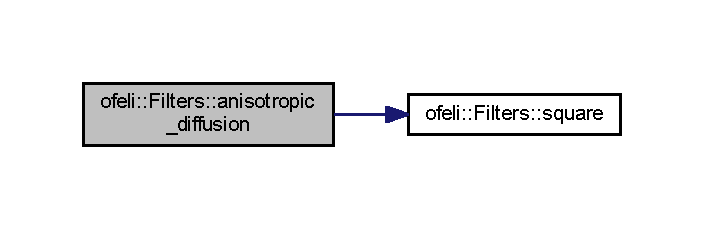
\includegraphics[width=338pt]{classofeli_1_1_filters_ae4a65a5259b3a91a523eefdf2d90b920_cgraph}
\end{center}
\end{figure}


\hypertarget{classofeli_1_1_filters_a0f29ec08c3d9febd2f95ba54ec88e524}{\index{ofeli\-::\-Filters@{ofeli\-::\-Filters}!morphological\-\_\-gradient\-\_\-yuv@{morphological\-\_\-gradient\-\_\-yuv}}
\index{morphological\-\_\-gradient\-\_\-yuv@{morphological\-\_\-gradient\-\_\-yuv}!ofeli::Filters@{ofeli\-::\-Filters}}
\subsubsection[{morphological\-\_\-gradient\-\_\-yuv}]{\setlength{\rightskip}{0pt plus 5cm}void ofeli\-::\-Filters\-::morphological\-\_\-gradient\-\_\-yuv (
\begin{DoxyParamCaption}
\item[{int}]{kernel\-\_\-length, }
\item[{int}]{alpha, }
\item[{int}]{beta, }
\item[{int}]{gamma}
\end{DoxyParamCaption}
)}}\label{classofeli_1_1_filters_a0f29ec08c3d9febd2f95ba54ec88e524}


Computes a morphological gradient \hyperlink{classofeli_1_1_filters_a9c02bc4005c55eeb5a426485af0d03a9}{gradient}. 

Gradient morphologique avec un élement structurant carré de taille kernel\-\_\-length. 

Definition at line 2755 of file filters.\-cpp.



The documentation for this class was generated from the following files\-:\begin{DoxyCompactItemize}
\item 
filters.\-hpp\item 
filters.\-cpp\end{DoxyCompactItemize}

\hypertarget{classofeli_1_1_geodesic_a_c}{\section{ofeli\-:\-:Geodesic\-A\-C Class Reference}
\label{classofeli_1_1_geodesic_a_c}\index{ofeli\-::\-Geodesic\-A\-C@{ofeli\-::\-Geodesic\-A\-C}}
}


{\ttfamily \#include $<$geodesic\-\_\-ac.\-hpp$>$}



Inheritance diagram for ofeli\-:\-:Geodesic\-A\-C\-:\nopagebreak
\begin{figure}[H]
\begin{center}
\leavevmode
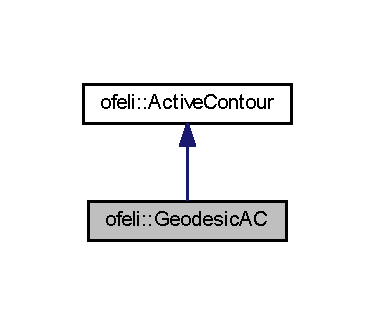
\includegraphics[width=180pt]{classofeli_1_1_geodesic_a_c__inherit__graph}
\end{center}
\end{figure}


Collaboration diagram for ofeli\-:\-:Geodesic\-A\-C\-:\nopagebreak
\begin{figure}[H]
\begin{center}
\leavevmode
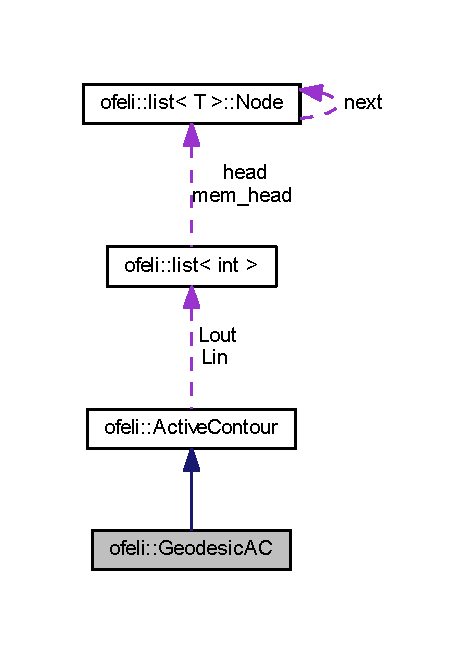
\includegraphics[width=224pt]{classofeli_1_1_geodesic_a_c__coll__graph}
\end{center}
\end{figure}
\subsection*{Public Member Functions}
\begin{DoxyCompactItemize}
\item 
\hypertarget{classofeli_1_1_geodesic_a_c_af7619ec4bd4c8b3a27e764054cbb5a57}{\hyperlink{classofeli_1_1_geodesic_a_c_af7619ec4bd4c8b3a27e764054cbb5a57}{Geodesic\-A\-C} (const unsigned char $\ast$img\-\_\-gradient\-\_\-data1, int img\-\_\-width1, int img\-\_\-height1)}\label{classofeli_1_1_geodesic_a_c_af7619ec4bd4c8b3a27e764054cbb5a57}

\begin{DoxyCompactList}\small\item\em Constructor to initialize the active contour with a centered rectangle and the default values of the algorithm parameters. \end{DoxyCompactList}\item 
\hyperlink{classofeli_1_1_geodesic_a_c_a460a9d62432ff49865c00e028b994252}{Geodesic\-A\-C} (const unsigned char $\ast$img\-\_\-gradient\-\_\-data1, int img\-\_\-width1, int img\-\_\-height1, bool has\-Ellipse1, double init\-\_\-width1, double init\-\_\-height1, double center\-\_\-x1, double center\-\_\-y1, bool has\-Cycle2\-\_\-1, int kernel\-\_\-length1, double sigma1, int Na1, int Ns1)
\begin{DoxyCompactList}\small\item\em Constructor to initialize the active contour from geometrical parameters of an unique shape, an ellipse or a rectangle. \end{DoxyCompactList}\item 
\hyperlink{classofeli_1_1_geodesic_a_c_a69faf0df5a2e9c8ce8128946bfb72653}{Geodesic\-A\-C} (const unsigned char $\ast$img\-\_\-gradient\-\_\-data1, int img\-\_\-width1, int img\-\_\-height1, const char $\ast$phi\-\_\-init1, bool has\-Cycle2\-\_\-1, int kernel\-\_\-length1, double sigma1, int Na1, int Ns1)
\begin{DoxyCompactList}\small\item\em Constructor to initialize the active contour from an initial phi level-\/set function. \end{DoxyCompactList}\item 
\hypertarget{classofeli_1_1_geodesic_a_c_af032dd46aec5735443cae0e04c2ea37a}{\hyperlink{classofeli_1_1_geodesic_a_c_af032dd46aec5735443cae0e04c2ea37a}{Geodesic\-A\-C} (const \hyperlink{classofeli_1_1_geodesic_a_c}{Geodesic\-A\-C} \&ac)}\label{classofeli_1_1_geodesic_a_c_af032dd46aec5735443cae0e04c2ea37a}

\begin{DoxyCompactList}\small\item\em Copy constructor. \end{DoxyCompactList}\item 
\hypertarget{classofeli_1_1_geodesic_a_c_a5f45547b45b9743a6fdf0388715dfcbc}{virtual void \hyperlink{classofeli_1_1_geodesic_a_c_a5f45547b45b9743a6fdf0388715dfcbc}{initialize\-\_\-for\-\_\-each\-\_\-frame} ()}\label{classofeli_1_1_geodesic_a_c_a5f45547b45b9743a6fdf0388715dfcbc}

\begin{DoxyCompactList}\small\item\em Initialization for each new frame buffer, used for video tracking. \end{DoxyCompactList}\item 
\hypertarget{classofeli_1_1_geodesic_a_c_ab2654dfef80654187878db4e961b2bfd}{unsigned char \hyperlink{classofeli_1_1_geodesic_a_c_ab2654dfef80654187878db4e961b2bfd}{get\-\_\-otsu\-\_\-threshold} () const }\label{classofeli_1_1_geodesic_a_c_ab2654dfef80654187878db4e961b2bfd}

\begin{DoxyCompactList}\small\item\em Getter function for \hyperlink{classofeli_1_1_geodesic_a_c_a1cde491f4e294413d5897e09fa0d3a39}{otsu\-\_\-threshold1}. \end{DoxyCompactList}\end{DoxyCompactItemize}
\subsection*{Private Member Functions}
\begin{DoxyCompactItemize}
\item 
virtual int \hyperlink{classofeli_1_1_geodesic_a_c_a1e4d1d3011526eaff49b5404f00f27f9}{compute\-\_\-external\-\_\-speed\-\_\-\-Fd} (int offset)
\begin{DoxyCompactList}\small\item\em Computes external speed {\itshape Fd} with a geodesic model for a current point {\itshape }(x,y) of \hyperlink{classofeli_1_1_active_contour_a31e0eb18a7ea6ae90acf66ed018fcd85}{Lout} or \hyperlink{classofeli_1_1_active_contour_a7662d4f5c8b87d3e642b08b7e341bd79}{Lin}. \end{DoxyCompactList}\item 
\hypertarget{classofeli_1_1_geodesic_a_c_a4cdf84261bfd4407e89984ea01f6c227}{bool \hyperlink{classofeli_1_1_geodesic_a_c_a4cdf84261bfd4407e89984ea01f6c227}{find\-\_\-direction\-\_\-evolution} ()}\label{classofeli_1_1_geodesic_a_c_a4cdf84261bfd4407e89984ea01f6c227}

\begin{DoxyCompactList}\small\item\em Calculates boolean \hyperlink{classofeli_1_1_geodesic_a_c_ada6b8ca4769ee7a03b0f47da3cbabc05}{is\-Inside}. \end{DoxyCompactList}\end{DoxyCompactItemize}
\subsection*{Static Private Member Functions}
\begin{DoxyCompactItemize}
\item 
\hypertarget{classofeli_1_1_geodesic_a_c_afab80d244aaf8d50902c9bb0de207bf2}{static unsigned char \hyperlink{classofeli_1_1_geodesic_a_c_afab80d244aaf8d50902c9bb0de207bf2}{otsu\-\_\-method} (const unsigned char $\ast$img\-\_\-data1, int img\-\_\-size1)}\label{classofeli_1_1_geodesic_a_c_afab80d244aaf8d50902c9bb0de207bf2}

\begin{DoxyCompactList}\small\item\em Otsu's method. \end{DoxyCompactList}\end{DoxyCompactItemize}
\subsection*{Private Attributes}
\begin{DoxyCompactItemize}
\item 
\hypertarget{classofeli_1_1_geodesic_a_c_a1cde491f4e294413d5897e09fa0d3a39}{const unsigned char \hyperlink{classofeli_1_1_geodesic_a_c_a1cde491f4e294413d5897e09fa0d3a39}{otsu\-\_\-threshold1}}\label{classofeli_1_1_geodesic_a_c_a1cde491f4e294413d5897e09fa0d3a39}

\begin{DoxyCompactList}\small\item\em Otsu's threshod of \hyperlink{classofeli_1_1_active_contour_a96480d79e9a60817925903da233a5b1e}{img\-\_\-data}. \end{DoxyCompactList}\item 
\hypertarget{classofeli_1_1_geodesic_a_c_ada6b8ca4769ee7a03b0f47da3cbabc05}{bool \hyperlink{classofeli_1_1_geodesic_a_c_ada6b8ca4769ee7a03b0f47da3cbabc05}{is\-Inside}}\label{classofeli_1_1_geodesic_a_c_ada6b8ca4769ee7a03b0f47da3cbabc05}

\begin{DoxyCompactList}\small\item\em Determines where are the high values of the gradient. \end{DoxyCompactList}\end{DoxyCompactItemize}
\subsection*{Additional Inherited Members}


\subsection{Detailed Description}
The child class \hyperlink{classofeli_1_1_geodesic_a_c}{Geodesic\-A\-C} implements a function to calculate specifically speed {\itshape Fd} based on a geodesic model, an edge-\/based energy functional. An Otsu's method is performed in order to find the high values of the gradient to converge even when the initialization of the curve is far of the solution. 

Definition at line 48 of file geodesic\-\_\-ac.\-hpp.



\subsection{Constructor \& Destructor Documentation}
\hypertarget{classofeli_1_1_geodesic_a_c_a460a9d62432ff49865c00e028b994252}{\index{ofeli\-::\-Geodesic\-A\-C@{ofeli\-::\-Geodesic\-A\-C}!Geodesic\-A\-C@{Geodesic\-A\-C}}
\index{Geodesic\-A\-C@{Geodesic\-A\-C}!ofeli::GeodesicAC@{ofeli\-::\-Geodesic\-A\-C}}
\subsubsection[{Geodesic\-A\-C}]{\setlength{\rightskip}{0pt plus 5cm}Geodesic\-A\-C\-::\-Geodesic\-A\-C (
\begin{DoxyParamCaption}
\item[{const unsigned char $\ast$}]{img\-\_\-gradient\-\_\-data1, }
\item[{int}]{img\-\_\-width1, }
\item[{int}]{img\-\_\-height1, }
\item[{bool}]{has\-Ellipse1, }
\item[{double}]{init\-\_\-width1, }
\item[{double}]{init\-\_\-height1, }
\item[{double}]{center\-\_\-x1, }
\item[{double}]{center\-\_\-y1, }
\item[{bool}]{has\-Cycle2\-\_\-1, }
\item[{int}]{kernel\-\_\-length1, }
\item[{double}]{sigma1, }
\item[{int}]{Na1, }
\item[{int}]{Ns1}
\end{DoxyParamCaption}
)}}\label{classofeli_1_1_geodesic_a_c_a460a9d62432ff49865c00e028b994252}


Constructor to initialize the active contour from geometrical parameters of an unique shape, an ellipse or a rectangle. 


\begin{DoxyParams}{Parameters}
{\em img\-\_\-gradient\-\_\-data1} & Input pointer on the grayscale image data buffer. Usually, this buffer is a smoothed gradient of an original image. This buffer must be row-\/wise. Passed to \hyperlink{classofeli_1_1_active_contour_a96480d79e9a60817925903da233a5b1e}{img\-\_\-data}. \\
\hline
{\em img\-\_\-width1} & Image width, i.\-e. number of columns. Passed to \hyperlink{classofeli_1_1_active_contour_a3623de7ebc0d27ba7fac21a5929afbc6}{img\-\_\-width}. \\
\hline
{\em img\-\_\-height1} & Image height, i.\-e. number of rows. Passed to \hyperlink{classofeli_1_1_active_contour_a88d02b47bab737ec97fe3a7ea9554c0c}{img\-\_\-height}. \\
\hline
{\em has\-Ellipse1} & Boolean to choose the shape of the active contour initialization, {\ttfamily true} for an ellipse or {\ttfamily false} for a rectangle. \\
\hline
{\em init\-\_\-width1} & Width of the shape divided by the image \hyperlink{classofeli_1_1_active_contour_a3623de7ebc0d27ba7fac21a5929afbc6}{img\-\_\-width}. \\
\hline
{\em init\-\_\-height1} & Height of the shape divided by the image \hyperlink{classofeli_1_1_active_contour_a88d02b47bab737ec97fe3a7ea9554c0c}{img\-\_\-height}. \\
\hline
{\em center\-\_\-x1} & X-\/axis position (or column index) of the center of the shape divided by the image \hyperlink{classofeli_1_1_active_contour_a3623de7ebc0d27ba7fac21a5929afbc6}{img\-\_\-width} subtracted by 0.\-5 \\
\hline
{\em center\-\_\-y1} & Y-\/axis position (or row index) of the center of the shape divided by the image \hyperlink{classofeli_1_1_active_contour_a88d02b47bab737ec97fe3a7ea9554c0c}{img\-\_\-height} subtracted by 0.\-5\par
 To have the center of the shape in the image \-: -\/0.\-5 $<$ center\-\_\-x1 $<$ 0.\-5 and -\/0.\-5 $<$ center\-\_\-y1 $<$ 0.\-5 \\
\hline
{\em has\-Cycle2\-\_\-1} & Boolean to have or not the curve smoothing, evolutions in the cycle 2 with an internal speed {\itshape Fint}. Passed to \hyperlink{classofeli_1_1_active_contour_aa763ff1bed211faa444013cbd5de0be3}{has\-Cycle2}. \\
\hline
{\em kernel\-\_\-length1} & Kernel length of the gaussian filter for the curve smoothing. Passed to \hyperlink{classofeli_1_1_active_contour_a2b32161d0a9ac64a4e4f4c242fabe27c}{kernel\-\_\-length}. \\
\hline
{\em sigma1} & Standard deviation of the gaussian kernel for the curve smoothing. Passed to \hyperlink{classofeli_1_1_active_contour_a66303b7f6b88270133462feb303b039a}{sigma}. \\
\hline
{\em Na1} & Number of times the active contour evolves in the cycle 1, external or data dependant evolutions with {\itshape Fd} speed. Passed to \hyperlink{classofeli_1_1_active_contour_a811a28ec9c39400d244783a8a2fe7e2d}{Na\-\_\-max}. \\
\hline
{\em Ns1} & Number of times the active contour evolves in the cycle 2, curve smoothing or internal evolutions with {\itshape Fint} speed. Passed to \hyperlink{classofeli_1_1_active_contour_a908322f93a50ce7808960236478649fe}{Ns\-\_\-max}. \\
\hline
\end{DoxyParams}


Definition at line 55 of file geodesic\-\_\-ac.\-cpp.



Here is the call graph for this function\-:\nopagebreak
\begin{figure}[H]
\begin{center}
\leavevmode
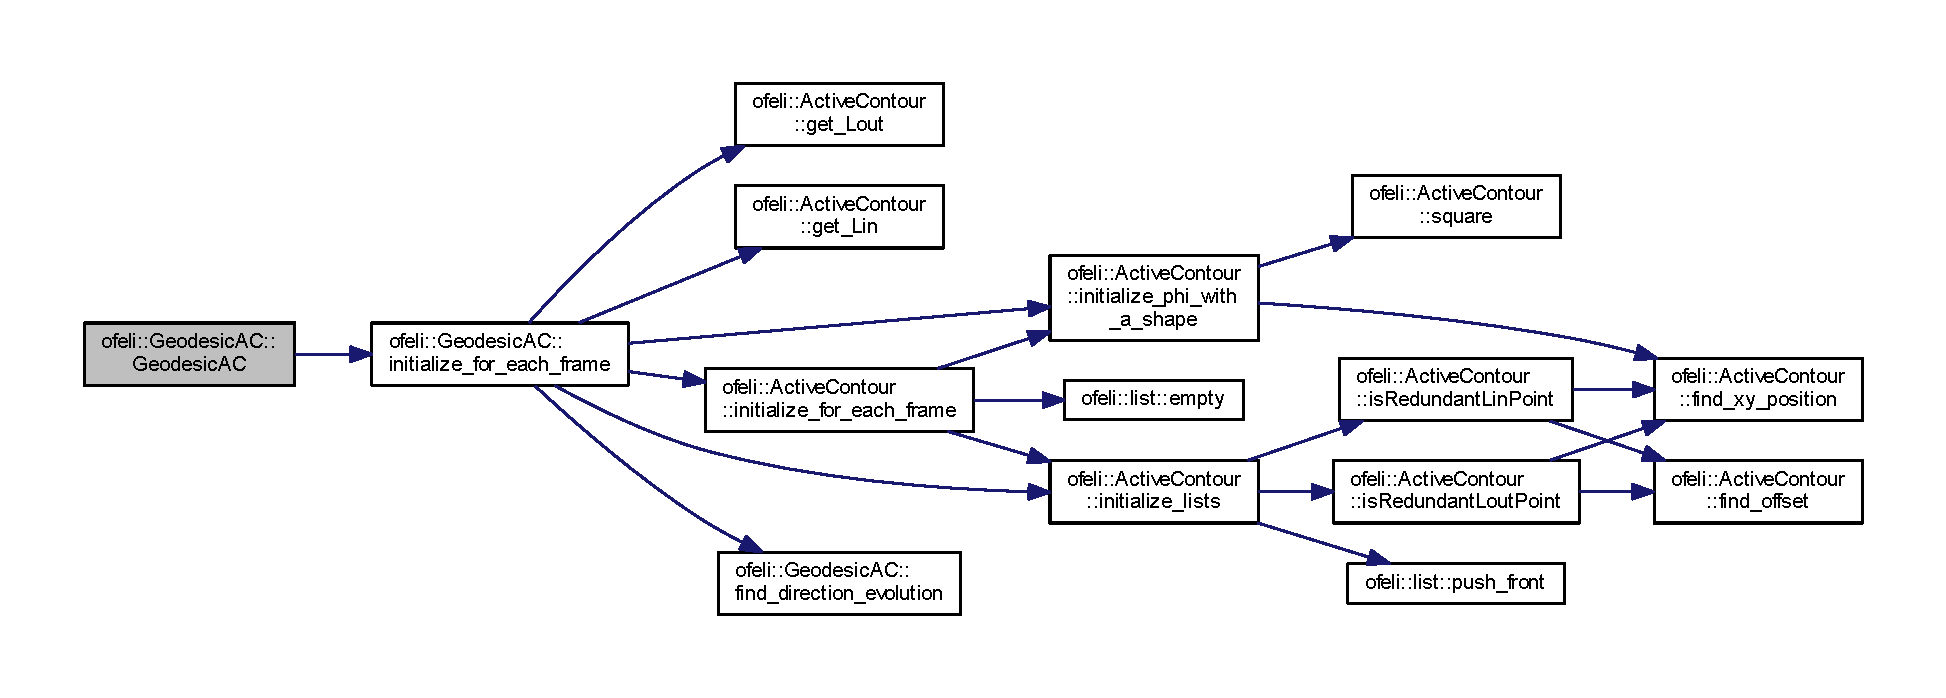
\includegraphics[width=350pt]{classofeli_1_1_geodesic_a_c_a460a9d62432ff49865c00e028b994252_cgraph}
\end{center}
\end{figure}


\hypertarget{classofeli_1_1_geodesic_a_c_a69faf0df5a2e9c8ce8128946bfb72653}{\index{ofeli\-::\-Geodesic\-A\-C@{ofeli\-::\-Geodesic\-A\-C}!Geodesic\-A\-C@{Geodesic\-A\-C}}
\index{Geodesic\-A\-C@{Geodesic\-A\-C}!ofeli::GeodesicAC@{ofeli\-::\-Geodesic\-A\-C}}
\subsubsection[{Geodesic\-A\-C}]{\setlength{\rightskip}{0pt plus 5cm}Geodesic\-A\-C\-::\-Geodesic\-A\-C (
\begin{DoxyParamCaption}
\item[{const unsigned char $\ast$}]{img\-\_\-gradient\-\_\-data1, }
\item[{int}]{img\-\_\-width1, }
\item[{int}]{img\-\_\-height1, }
\item[{const char $\ast$}]{phi\-\_\-init1, }
\item[{bool}]{has\-Cycle2\-\_\-1, }
\item[{int}]{kernel\-\_\-length1, }
\item[{double}]{sigma1, }
\item[{int}]{Na1, }
\item[{int}]{Ns1}
\end{DoxyParamCaption}
)}}\label{classofeli_1_1_geodesic_a_c_a69faf0df5a2e9c8ce8128946bfb72653}


Constructor to initialize the active contour from an initial phi level-\/set function. 


\begin{DoxyParams}{Parameters}
{\em img\-\_\-gradient\-\_\-data1} & Input pointer on the grayscale image data buffer. Usually, this buffer is a smoothed gradient of an original image. This buffer must be row-\/wise. Passed to \hyperlink{classofeli_1_1_active_contour_a96480d79e9a60817925903da233a5b1e}{img\-\_\-data}. \\
\hline
{\em img\-\_\-width1} & Image width, i.\-e. number of columns. Passed to \hyperlink{classofeli_1_1_active_contour_a3623de7ebc0d27ba7fac21a5929afbc6}{img\-\_\-width}. \\
\hline
{\em img\-\_\-height1} & Image height, i.\-e. number of rows. Passed to \hyperlink{classofeli_1_1_active_contour_a88d02b47bab737ec97fe3a7ea9554c0c}{img\-\_\-height}. \\
\hline
{\em phi\-\_\-init1} & Pointer on the initialized level-\/set function buffer. Copied to \hyperlink{classofeli_1_1_active_contour_aacb03a6ded4ca51cb52f58aeff955ef7}{phi}. \\
\hline
{\em has\-Cycle2\-\_\-1} & Boolean to have or not the curve smoothing, evolutions in the cycle 2 with an internal speed {\itshape Fint}. Passed to \hyperlink{classofeli_1_1_active_contour_aa763ff1bed211faa444013cbd5de0be3}{has\-Cycle2}. \\
\hline
{\em kernel\-\_\-length1} & Kernel length of the gaussian filter for the curve smoothing. Passed to \hyperlink{classofeli_1_1_active_contour_a2b32161d0a9ac64a4e4f4c242fabe27c}{kernel\-\_\-length}. \\
\hline
{\em sigma1} & Standard deviation of the gaussian kernel for the curve smoothing. Passed to \hyperlink{classofeli_1_1_active_contour_a66303b7f6b88270133462feb303b039a}{sigma}. \\
\hline
{\em Na1} & Number of times the active contour evolves in the cycle 1, external or data dependant evolutions with {\itshape Fd} speed. Passed to \hyperlink{classofeli_1_1_active_contour_a811a28ec9c39400d244783a8a2fe7e2d}{Na\-\_\-max}. \\
\hline
{\em Ns1} & Number of times the active contour evolves in the cycle 2, curve smoothing or internal evolutions with {\itshape Fint} speed. Passed to \hyperlink{classofeli_1_1_active_contour_a908322f93a50ce7808960236478649fe}{Ns\-\_\-max}. \\
\hline
\end{DoxyParams}


Definition at line 67 of file geodesic\-\_\-ac.\-cpp.



Here is the call graph for this function\-:\nopagebreak
\begin{figure}[H]
\begin{center}
\leavevmode
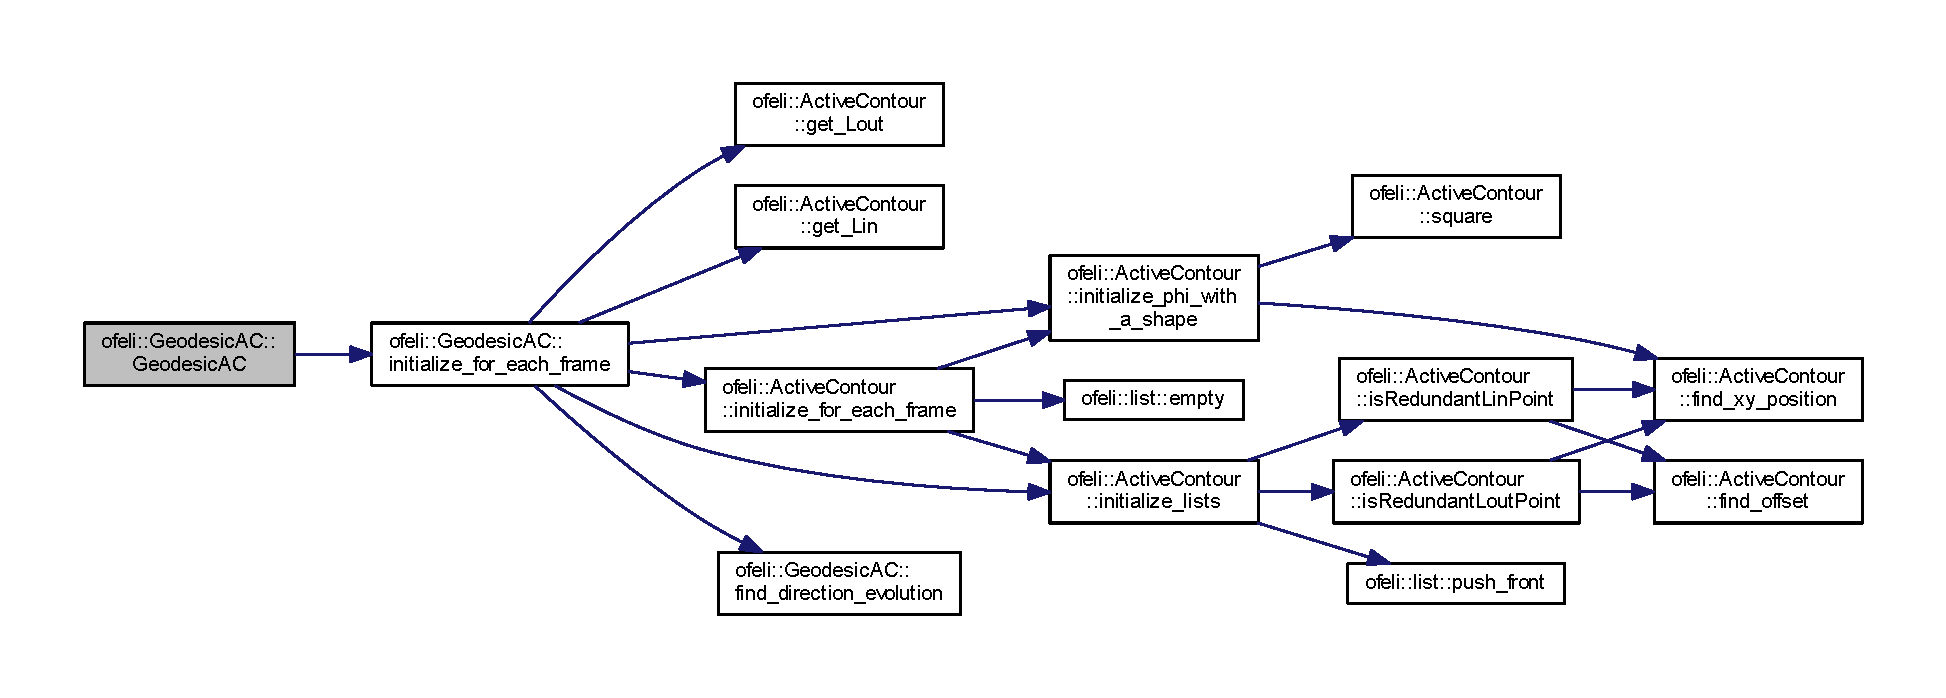
\includegraphics[width=350pt]{classofeli_1_1_geodesic_a_c_a69faf0df5a2e9c8ce8128946bfb72653_cgraph}
\end{center}
\end{figure}




\subsection{Member Function Documentation}
\hypertarget{classofeli_1_1_geodesic_a_c_a1e4d1d3011526eaff49b5404f00f27f9}{\index{ofeli\-::\-Geodesic\-A\-C@{ofeli\-::\-Geodesic\-A\-C}!compute\-\_\-external\-\_\-speed\-\_\-\-Fd@{compute\-\_\-external\-\_\-speed\-\_\-\-Fd}}
\index{compute\-\_\-external\-\_\-speed\-\_\-\-Fd@{compute\-\_\-external\-\_\-speed\-\_\-\-Fd}!ofeli::GeodesicAC@{ofeli\-::\-Geodesic\-A\-C}}
\subsubsection[{compute\-\_\-external\-\_\-speed\-\_\-\-Fd}]{\setlength{\rightskip}{0pt plus 5cm}int Geodesic\-A\-C\-::compute\-\_\-external\-\_\-speed\-\_\-\-Fd (
\begin{DoxyParamCaption}
\item[{int}]{offset}
\end{DoxyParamCaption}
)\hspace{0.3cm}{\ttfamily [private]}, {\ttfamily [virtual]}}}\label{classofeli_1_1_geodesic_a_c_a1e4d1d3011526eaff49b5404f00f27f9}


Computes external speed {\itshape Fd} with a geodesic model for a current point {\itshape }(x,y) of \hyperlink{classofeli_1_1_active_contour_a31e0eb18a7ea6ae90acf66ed018fcd85}{Lout} or \hyperlink{classofeli_1_1_active_contour_a7662d4f5c8b87d3e642b08b7e341bd79}{Lin}. 


\begin{DoxyParams}{Parameters}
{\em offset} & offset of the image data buffer with {\itshape offset} = {\itshape x} + {\itshape y} × \hyperlink{classofeli_1_1_active_contour_a3623de7ebc0d27ba7fac21a5929afbc6}{img\-\_\-width} \\
\hline
\end{DoxyParams}


Reimplemented from \hyperlink{classofeli_1_1_active_contour_ae3871b40f2f3e27ae0d75775798cdee1}{ofeli\-::\-Active\-Contour}.



Definition at line 105 of file geodesic\-\_\-ac.\-cpp.



Here is the call graph for this function\-:\nopagebreak
\begin{figure}[H]
\begin{center}
\leavevmode
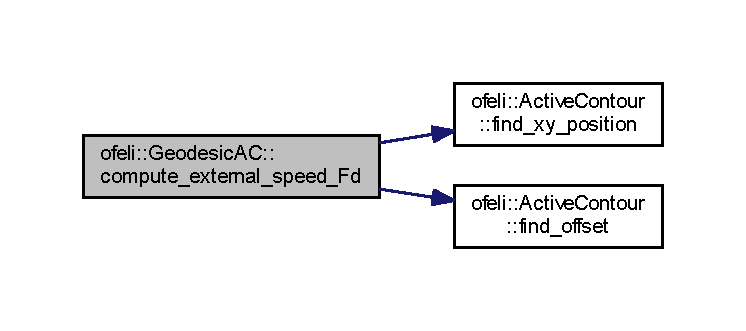
\includegraphics[width=350pt]{classofeli_1_1_geodesic_a_c_a1e4d1d3011526eaff49b5404f00f27f9_cgraph}
\end{center}
\end{figure}




The documentation for this class was generated from the following files\-:\begin{DoxyCompactItemize}
\item 
geodesic\-\_\-ac.\-hpp\item 
geodesic\-\_\-ac.\-cpp\end{DoxyCompactItemize}

\hypertarget{structofeli_1_1greater}{\section{ofeli\-:\-:greater$<$ T $>$ Struct Template Reference}
\label{structofeli_1_1greater}\index{ofeli\-::greater$<$ T $>$@{ofeli\-::greater$<$ T $>$}}
}


{\ttfamily \#include $<$linked\-\_\-list.\-hpp$>$}

\subsection*{Public Member Functions}
\begin{DoxyCompactItemize}
\item 
\hypertarget{structofeli_1_1greater_a9aaddf2c494e306c8c6d823d8b2dacf0}{bool {\bfseries operator()} (const T \&x, const T \&y) const }\label{structofeli_1_1greater_a9aaddf2c494e306c8c6d823d8b2dacf0}

\end{DoxyCompactItemize}


\subsection{Detailed Description}
\subsubsection*{template$<$typename T = int$>$struct ofeli\-::greater$<$ T $>$}

This class defines function objects for the \char`\"{}greater than\char`\"{} inequality comparison operation. Generically, function objects are instances of a class with member function {\ttfamily operator()} defined. This member function allows the object to be used with the same syntax as a regular function call, and therefore it can be used in templates instead of a pointer to a function. {\ttfamily greater} has its {\ttfamily operator()} member defined such that it returns {\ttfamily true} if its first argument compares greater than the second one using {\ttfamily operator$>$}, and {\ttfamily false} otherwise. This class can be used with the template function $<$\-T$>$\-::sort(\-Binary\-Predicate compare). 

Definition at line 382 of file linked\-\_\-list.\-hpp.



The documentation for this struct was generated from the following file\-:\begin{DoxyCompactItemize}
\item 
linked\-\_\-list.\-hpp\end{DoxyCompactItemize}

\hypertarget{structofeli_1_1greater__equal}{\section{ofeli\-:\-:greater\-\_\-equal$<$ T $>$ Struct Template Reference}
\label{structofeli_1_1greater__equal}\index{ofeli\-::greater\-\_\-equal$<$ T $>$@{ofeli\-::greater\-\_\-equal$<$ T $>$}}
}


{\ttfamily \#include $<$linked\-\_\-list.\-hpp$>$}

\subsection*{Public Member Functions}
\begin{DoxyCompactItemize}
\item 
\hypertarget{structofeli_1_1greater__equal_a5042ca3313adcc116ad2394b7aaacacc}{bool {\bfseries operator()} (const T \&x, const T \&y) const }\label{structofeli_1_1greater__equal_a5042ca3313adcc116ad2394b7aaacacc}

\end{DoxyCompactItemize}


\subsection{Detailed Description}
\subsubsection*{template$<$typename T = int$>$struct ofeli\-::greater\-\_\-equal$<$ T $>$}

This class defines function objects for the \char`\"{}greater than or equal to\char`\"{} comparison operation ($>$=). Generically, function objects are instances of a class with member function {\ttfamily operator()} defined. This member function allows the object to be used with the same syntax as a regular function call, and therefore it can be used in templates instead of a pointer to a function. {\ttfamily \hyperlink{structofeli_1_1greater__equal}{greater\-\_\-equal}} has its {\ttfamily operator()} member defined such that it returns {\ttfamily true} if its first argument compares greater than or equal to the second one using {\ttfamily operator$>$=}, and {\ttfamily false} otherwise. This class can be used with the template function {\ttfamily \hyperlink{classofeli_1_1list_aaeedac18b70d233644d84c7ad3a9a3fa}{list$<$\-T$>$\-::sort(\-Binary\-Predicate compare)}}. 

Definition at line 388 of file linked\-\_\-list.\-hpp.



The documentation for this struct was generated from the following file\-:\begin{DoxyCompactItemize}
\item 
linked\-\_\-list.\-hpp\end{DoxyCompactItemize}

\hypertarget{classofeli_1_1_hausdorff_distance}{\section{ofeli\-:\-:Hausdorff\-Distance Class Reference}
\label{classofeli_1_1_hausdorff_distance}\index{ofeli\-::\-Hausdorff\-Distance@{ofeli\-::\-Hausdorff\-Distance}}
}


{\ttfamily \#include $<$hausdorff\-\_\-distance.\-hpp$>$}

\subsection*{Public Member Functions}
\begin{DoxyCompactItemize}
\item 
\hypertarget{classofeli_1_1_hausdorff_distance_a4b1864bb0503e1a3b85bc75100ec1c91}{\hyperlink{classofeli_1_1_hausdorff_distance_a4b1864bb0503e1a3b85bc75100ec1c91}{Hausdorff\-Distance} (const int $\ast$list1\-\_\-1, int list1\-\_\-1\-\_\-length, int img1\-\_\-1\-\_\-width, int img1\-\_\-1\-\_\-height, const int $\ast$list2\-\_\-1, int list2\-\_\-1\-\_\-length, int img2\-\_\-1\-\_\-width, int img2\-\_\-1\-\_\-height)}\label{classofeli_1_1_hausdorff_distance_a4b1864bb0503e1a3b85bc75100ec1c91}

\begin{DoxyCompactList}\small\item\em Constructor considering lists A and B to compare and their sizes and image dimensions. All calculations are done in the construcor. \end{DoxyCompactList}\item 
\hypertarget{classofeli_1_1_hausdorff_distance_aeb09d86b41a000db23138bbd8e2fdd76}{double \hyperlink{classofeli_1_1_hausdorff_distance_aeb09d86b41a000db23138bbd8e2fdd76}{get\-\_\-hausdorff\-\_\-dist} () const }\label{classofeli_1_1_hausdorff_distance_aeb09d86b41a000db23138bbd8e2fdd76}

\begin{DoxyCompactList}\small\item\em Getter function for \hyperlink{classofeli_1_1_hausdorff_distance_a895012cca75a4f37ff0ef376dca57581}{hausdorff\-\_\-dist}. \end{DoxyCompactList}\item 
\hypertarget{classofeli_1_1_hausdorff_distance_a39798b7b04918d27059f9d93f1c3ac7c}{double \hyperlink{classofeli_1_1_hausdorff_distance_a39798b7b04918d27059f9d93f1c3ac7c}{get\-\_\-modified\-\_\-hausdorff\-\_\-dist} () const }\label{classofeli_1_1_hausdorff_distance_a39798b7b04918d27059f9d93f1c3ac7c}

\begin{DoxyCompactList}\small\item\em Getter function for \hyperlink{classofeli_1_1_hausdorff_distance_a895012cca75a4f37ff0ef376dca57581}{hausdorff\-\_\-dist}. \end{DoxyCompactList}\item 
\hypertarget{classofeli_1_1_hausdorff_distance_aa944abda5343393a0f0193aacb9188c3}{double \hyperlink{classofeli_1_1_hausdorff_distance_aa944abda5343393a0f0193aacb9188c3}{get\-\_\-hausdorff\-\_\-ratio} () const }\label{classofeli_1_1_hausdorff_distance_aa944abda5343393a0f0193aacb9188c3}

\begin{DoxyCompactList}\small\item\em Getter function for \hyperlink{classofeli_1_1_hausdorff_distance_a677f05cee335e19aaf4b931a75fd969c}{hausdorff\-\_\-ratio}. \end{DoxyCompactList}\item 
\hypertarget{classofeli_1_1_hausdorff_distance_af965376bb737c524ab3589e1637f17c9}{double \hyperlink{classofeli_1_1_hausdorff_distance_af965376bb737c524ab3589e1637f17c9}{get\-\_\-modified\-\_\-hausdorff\-\_\-ratio} () const }\label{classofeli_1_1_hausdorff_distance_af965376bb737c524ab3589e1637f17c9}

\begin{DoxyCompactList}\small\item\em Getter function for \hyperlink{classofeli_1_1_hausdorff_distance_aa567ae532fb26c06648463ed3e0db0c6}{modified\-\_\-hausdorff\-\_\-dist}. \end{DoxyCompactList}\item 
\hypertarget{classofeli_1_1_hausdorff_distance_ad0f1da8d98faaeda902470c89d321960}{double \hyperlink{classofeli_1_1_hausdorff_distance_ad0f1da8d98faaeda902470c89d321960}{get\-\_\-centroids\-\_\-dist} () const }\label{classofeli_1_1_hausdorff_distance_ad0f1da8d98faaeda902470c89d321960}

\begin{DoxyCompactList}\small\item\em Getter function for \hyperlink{classofeli_1_1_hausdorff_distance_a6e20d6be78d947d732eefb5d207cbaab}{centroids\-\_\-dist}. \end{DoxyCompactList}\item 
\hypertarget{classofeli_1_1_hausdorff_distance_af383f704380a7e9eb3c4e2ec8bb047da}{double \hyperlink{classofeli_1_1_hausdorff_distance_af383f704380a7e9eb3c4e2ec8bb047da}{get\-\_\-centroids\-\_\-ratio} () const }\label{classofeli_1_1_hausdorff_distance_af383f704380a7e9eb3c4e2ec8bb047da}

\begin{DoxyCompactList}\small\item\em Getter function for \hyperlink{classofeli_1_1_hausdorff_distance_ae0d112616201086a7480541b3ccaa62e}{centroids\-\_\-ratio}. \end{DoxyCompactList}\end{DoxyCompactItemize}
\subsection*{Private Member Functions}
\begin{DoxyCompactItemize}
\item 
\hypertarget{classofeli_1_1_hausdorff_distance_a60cd38cf5ac504a49fdae5aa8c1f5daa}{void \hyperlink{classofeli_1_1_hausdorff_distance_a60cd38cf5ac504a49fdae5aa8c1f5daa}{compute\-\_\-hausdorff\-\_\-dist} (double \&\hyperlink{classofeli_1_1_hausdorff_distance_a895012cca75a4f37ff0ef376dca57581}{hausdorff\-\_\-dist}, double \&\hyperlink{classofeli_1_1_hausdorff_distance_aa567ae532fb26c06648463ed3e0db0c6}{modified\-\_\-hausdorff\-\_\-dist}) const }\label{classofeli_1_1_hausdorff_distance_a60cd38cf5ac504a49fdae5aa8c1f5daa}

\begin{DoxyCompactList}\small\item\em Computes the distances \hyperlink{classofeli_1_1_hausdorff_distance_a895012cca75a4f37ff0ef376dca57581}{hausdorff\-\_\-dist} and \hyperlink{classofeli_1_1_hausdorff_distance_aa567ae532fb26c06648463ed3e0db0c6}{modified\-\_\-hausdorff\-\_\-dist} between \hyperlink{classofeli_1_1_hausdorff_distance_a363ef19e82b2743e828ec0a613b81a1d}{list1} and \hyperlink{classofeli_1_1_hausdorff_distance_a214f70f274ec1099b0b3fda1e5060c1f}{list2}. \end{DoxyCompactList}\item 
\hypertarget{classofeli_1_1_hausdorff_distance_a86ce0a178063d6d80c5c4d8dd89bf7c0}{void \hyperlink{classofeli_1_1_hausdorff_distance_a86ce0a178063d6d80c5c4d8dd89bf7c0}{swap\-\_\-lists} ()}\label{classofeli_1_1_hausdorff_distance_a86ce0a178063d6d80c5c4d8dd89bf7c0}

\begin{DoxyCompactList}\small\item\em Swaps lists to compute the backward distances. \end{DoxyCompactList}\end{DoxyCompactItemize}
\subsection*{Static Private Member Functions}
\begin{DoxyCompactItemize}
\item 
\hypertarget{classofeli_1_1_hausdorff_distance_ad6b75e3f7e4bedbd8eb9a280d25d4d21}{static double \hyperlink{classofeli_1_1_hausdorff_distance_ad6b75e3f7e4bedbd8eb9a280d25d4d21}{calculate\-\_\-max\-\_\-dist} (int width1, int height1, int width2, int height2)}\label{classofeli_1_1_hausdorff_distance_ad6b75e3f7e4bedbd8eb9a280d25d4d21}

\begin{DoxyCompactList}\small\item\em Calculates the maximum ditance. \end{DoxyCompactList}\item 
\hypertarget{classofeli_1_1_hausdorff_distance_a96693bddcceb4086bc8da73a0db696d8}{{\footnotesize template$<$typename T $>$ }\\static T \hyperlink{classofeli_1_1_hausdorff_distance_a96693bddcceb4086bc8da73a0db696d8}{square} (const T \&value)}\label{classofeli_1_1_hausdorff_distance_a96693bddcceb4086bc8da73a0db696d8}

\begin{DoxyCompactList}\small\item\em Gives the square of a value. \end{DoxyCompactList}\end{DoxyCompactItemize}
\subsection*{Private Attributes}
\begin{DoxyCompactItemize}
\item 
\hypertarget{classofeli_1_1_hausdorff_distance_a363ef19e82b2743e828ec0a613b81a1d}{const int $\ast$ \hyperlink{classofeli_1_1_hausdorff_distance_a363ef19e82b2743e828ec0a613b81a1d}{list1}}\label{classofeli_1_1_hausdorff_distance_a363ef19e82b2743e828ec0a613b81a1d}

\begin{DoxyCompactList}\small\item\em Pointer on a array containing the pixels' offsets of a boundary segmentation from an image data buffer {\itshape img1}. \end{DoxyCompactList}\item 
\hypertarget{classofeli_1_1_hausdorff_distance_afc53a51bbfac8467c349c50be57e3145}{int \hyperlink{classofeli_1_1_hausdorff_distance_afc53a51bbfac8467c349c50be57e3145}{list1\-\_\-length}}\label{classofeli_1_1_hausdorff_distance_afc53a51bbfac8467c349c50be57e3145}

\begin{DoxyCompactList}\small\item\em Length of the array pointed by \hyperlink{classofeli_1_1_hausdorff_distance_a363ef19e82b2743e828ec0a613b81a1d}{list1}. \end{DoxyCompactList}\item 
\hypertarget{classofeli_1_1_hausdorff_distance_a08a977f3abbb359c8f908b4df821c901}{int \hyperlink{classofeli_1_1_hausdorff_distance_a08a977f3abbb359c8f908b4df821c901}{img1\-\_\-width}}\label{classofeli_1_1_hausdorff_distance_a08a977f3abbb359c8f908b4df821c901}

\begin{DoxyCompactList}\small\item\em {\itshape img1} width, i.\-e. number of columns of {\itshape img1}. \end{DoxyCompactList}\item 
\hypertarget{classofeli_1_1_hausdorff_distance_af0c40e9fa7899ecd56147691be6b0399}{int \hyperlink{classofeli_1_1_hausdorff_distance_af0c40e9fa7899ecd56147691be6b0399}{img1\-\_\-height}}\label{classofeli_1_1_hausdorff_distance_af0c40e9fa7899ecd56147691be6b0399}

\begin{DoxyCompactList}\small\item\em {\itshape img1} height, i.\-e. number of rows of {\itshape img1}. \end{DoxyCompactList}\item 
\hypertarget{classofeli_1_1_hausdorff_distance_a214f70f274ec1099b0b3fda1e5060c1f}{const int $\ast$ \hyperlink{classofeli_1_1_hausdorff_distance_a214f70f274ec1099b0b3fda1e5060c1f}{list2}}\label{classofeli_1_1_hausdorff_distance_a214f70f274ec1099b0b3fda1e5060c1f}

\begin{DoxyCompactList}\small\item\em Pointer on a array containing the pixels' offsets of boundary segmentation from an image data buffer {\itshape img2}. \end{DoxyCompactList}\item 
\hypertarget{classofeli_1_1_hausdorff_distance_af722dd3132298fa7113e897129e587b3}{int \hyperlink{classofeli_1_1_hausdorff_distance_af722dd3132298fa7113e897129e587b3}{list2\-\_\-length}}\label{classofeli_1_1_hausdorff_distance_af722dd3132298fa7113e897129e587b3}

\begin{DoxyCompactList}\small\item\em Length of the array pointed by \hyperlink{classofeli_1_1_hausdorff_distance_a214f70f274ec1099b0b3fda1e5060c1f}{list2}. \end{DoxyCompactList}\item 
\hypertarget{classofeli_1_1_hausdorff_distance_a923f35c5cec18e61eae71f1e0a7b139f}{int \hyperlink{classofeli_1_1_hausdorff_distance_a923f35c5cec18e61eae71f1e0a7b139f}{img2\-\_\-width}}\label{classofeli_1_1_hausdorff_distance_a923f35c5cec18e61eae71f1e0a7b139f}

\begin{DoxyCompactList}\small\item\em {\itshape img2} width, i.\-e. number of columns of {\itshape img2}. \end{DoxyCompactList}\item 
\hypertarget{classofeli_1_1_hausdorff_distance_aa5e3dd2eff7f1302e861a294c7a92f44}{int \hyperlink{classofeli_1_1_hausdorff_distance_aa5e3dd2eff7f1302e861a294c7a92f44}{img2\-\_\-height}}\label{classofeli_1_1_hausdorff_distance_aa5e3dd2eff7f1302e861a294c7a92f44}

\begin{DoxyCompactList}\small\item\em img2 height, i.\-e. number of rows of img2. \end{DoxyCompactList}\item 
\hypertarget{classofeli_1_1_hausdorff_distance_a70e3c0b9d2d8ce97529266fbbae92338}{double \hyperlink{classofeli_1_1_hausdorff_distance_a70e3c0b9d2d8ce97529266fbbae92338}{mean\-\_\-x1}}\label{classofeli_1_1_hausdorff_distance_a70e3c0b9d2d8ce97529266fbbae92338}

\begin{DoxyCompactList}\small\item\em Mean position of list1 in the X-\/axis. \end{DoxyCompactList}\item 
\hypertarget{classofeli_1_1_hausdorff_distance_a493c07736724a1cc41124517242f767b}{double \hyperlink{classofeli_1_1_hausdorff_distance_a493c07736724a1cc41124517242f767b}{mean\-\_\-y1}}\label{classofeli_1_1_hausdorff_distance_a493c07736724a1cc41124517242f767b}

\begin{DoxyCompactList}\small\item\em Mean position of list1 in the Y-\/axis. \end{DoxyCompactList}\item 
\hypertarget{classofeli_1_1_hausdorff_distance_a068a35f111926abadb330c15a4d37d6a}{double \hyperlink{classofeli_1_1_hausdorff_distance_a068a35f111926abadb330c15a4d37d6a}{mean\-\_\-x2}}\label{classofeli_1_1_hausdorff_distance_a068a35f111926abadb330c15a4d37d6a}

\begin{DoxyCompactList}\small\item\em Mean position of list2 in the X-\/axis. \end{DoxyCompactList}\item 
\hypertarget{classofeli_1_1_hausdorff_distance_ac9edb4911499fa08e0adf8f08638cf30}{double \hyperlink{classofeli_1_1_hausdorff_distance_ac9edb4911499fa08e0adf8f08638cf30}{mean\-\_\-y2}}\label{classofeli_1_1_hausdorff_distance_ac9edb4911499fa08e0adf8f08638cf30}

\begin{DoxyCompactList}\small\item\em Mean position of list2 in the Y-\/axis. \end{DoxyCompactList}\item 
\hypertarget{classofeli_1_1_hausdorff_distance_a08abc6a0ea807a4f1eb500b159b5c34d}{const double \hyperlink{classofeli_1_1_hausdorff_distance_a08abc6a0ea807a4f1eb500b159b5c34d}{max\-\_\-dist}}\label{classofeli_1_1_hausdorff_distance_a08abc6a0ea807a4f1eb500b159b5c34d}

\begin{DoxyCompactList}\small\item\em Maximum distance or diagonal of the images. \end{DoxyCompactList}\item 
\hypertarget{classofeli_1_1_hausdorff_distance_a895012cca75a4f37ff0ef376dca57581}{double \hyperlink{classofeli_1_1_hausdorff_distance_a895012cca75a4f37ff0ef376dca57581}{hausdorff\-\_\-dist}}\label{classofeli_1_1_hausdorff_distance_a895012cca75a4f37ff0ef376dca57581}

\begin{DoxyCompactList}\small\item\em Hausdorff distance, i.\-e. max( min(distance) ). \end{DoxyCompactList}\item 
\hypertarget{classofeli_1_1_hausdorff_distance_a677f05cee335e19aaf4b931a75fd969c}{double \hyperlink{classofeli_1_1_hausdorff_distance_a677f05cee335e19aaf4b931a75fd969c}{hausdorff\-\_\-ratio}}\label{classofeli_1_1_hausdorff_distance_a677f05cee335e19aaf4b931a75fd969c}

\begin{DoxyCompactList}\small\item\em Hausdorff distance divides by max\-\_\-dist. \end{DoxyCompactList}\item 
\hypertarget{classofeli_1_1_hausdorff_distance_aa567ae532fb26c06648463ed3e0db0c6}{double \hyperlink{classofeli_1_1_hausdorff_distance_aa567ae532fb26c06648463ed3e0db0c6}{modified\-\_\-hausdorff\-\_\-dist}}\label{classofeli_1_1_hausdorff_distance_aa567ae532fb26c06648463ed3e0db0c6}

\begin{DoxyCompactList}\small\item\em Modified Hausdorff distance, i.\-e mean( min(distance) ). \end{DoxyCompactList}\item 
\hypertarget{classofeli_1_1_hausdorff_distance_ac7325ec0abebea6745ce9af9dbcbfe60}{double \hyperlink{classofeli_1_1_hausdorff_distance_ac7325ec0abebea6745ce9af9dbcbfe60}{modified\-\_\-hausdorff\-\_\-ratio}}\label{classofeli_1_1_hausdorff_distance_ac7325ec0abebea6745ce9af9dbcbfe60}

\begin{DoxyCompactList}\small\item\em Modified Hausdorff distance divides by max\-\_\-dist. \end{DoxyCompactList}\item 
\hypertarget{classofeli_1_1_hausdorff_distance_a6e20d6be78d947d732eefb5d207cbaab}{double \hyperlink{classofeli_1_1_hausdorff_distance_a6e20d6be78d947d732eefb5d207cbaab}{centroids\-\_\-dist}}\label{classofeli_1_1_hausdorff_distance_a6e20d6be78d947d732eefb5d207cbaab}

\begin{DoxyCompactList}\small\item\em Distance between the centroids of the lists. \end{DoxyCompactList}\item 
\hypertarget{classofeli_1_1_hausdorff_distance_ae0d112616201086a7480541b3ccaa62e}{double \hyperlink{classofeli_1_1_hausdorff_distance_ae0d112616201086a7480541b3ccaa62e}{centroids\-\_\-ratio}}\label{classofeli_1_1_hausdorff_distance_ae0d112616201086a7480541b3ccaa62e}

\begin{DoxyCompactList}\small\item\em Distance between the centroids of the lists divides by max\-\_\-dist. \end{DoxyCompactList}\end{DoxyCompactItemize}


\subsection{Detailed Description}
The class \hyperlink{classofeli_1_1_hausdorff_distance}{Hausdorff\-Distance} computes the Hausdorff distance and the modified Hausdorff distance from two arrays of points which contain the pixels' offsets of a boundary segmentation. 

Definition at line 46 of file hausdorff\-\_\-distance.\-hpp.



The documentation for this class was generated from the following files\-:\begin{DoxyCompactItemize}
\item 
hausdorff\-\_\-distance.\-hpp\item 
hausdorff\-\_\-distance.\-cpp\end{DoxyCompactItemize}

\hypertarget{classofeli_1_1_image_viewer}{\section{ofeli\-:\-:Image\-Viewer Class Reference}
\label{classofeli_1_1_image_viewer}\index{ofeli\-::\-Image\-Viewer@{ofeli\-::\-Image\-Viewer}}
}


{\ttfamily \#include $<$imageviewer.\-hpp$>$}



Inheritance diagram for ofeli\-:\-:Image\-Viewer\-:\nopagebreak
\begin{figure}[H]
\begin{center}
\leavevmode
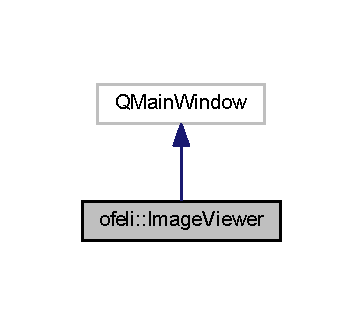
\includegraphics[width=174pt]{classofeli_1_1_image_viewer__inherit__graph}
\end{center}
\end{figure}


Collaboration diagram for ofeli\-:\-:Image\-Viewer\-:\nopagebreak
\begin{figure}[H]
\begin{center}
\leavevmode
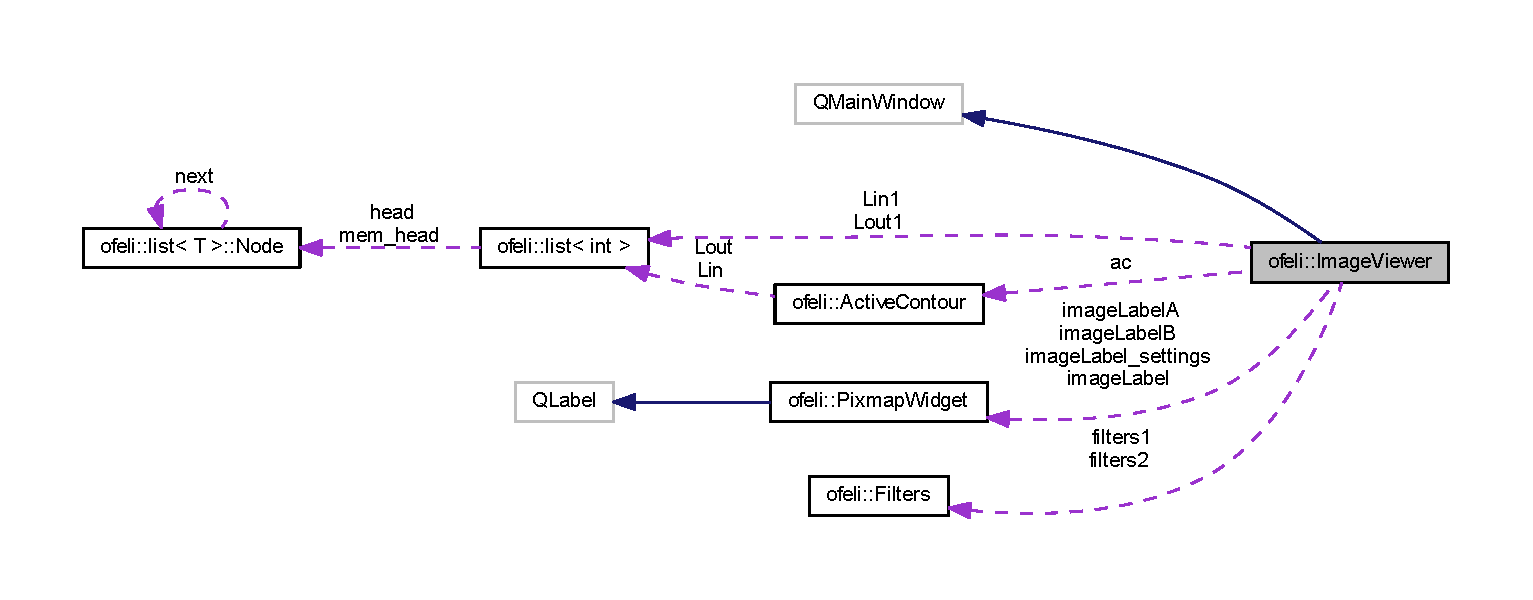
\includegraphics[width=350pt]{classofeli_1_1_image_viewer__coll__graph}
\end{center}
\end{figure}
\subsection*{Signals}
\begin{DoxyCompactItemize}
\item 
\hypertarget{classofeli_1_1_image_viewer_a524fa87199b9a93d35a686a4aa508f85}{void {\bfseries changed} (const Q\-Mime\-Data $\ast$mime\-Data=0)}\label{classofeli_1_1_image_viewer_a524fa87199b9a93d35a686a4aa508f85}

\end{DoxyCompactItemize}
\subsection*{Public Member Functions}
\begin{DoxyCompactItemize}
\item 
\hypertarget{classofeli_1_1_image_viewer_ad43b24d179c58e710b55fda869cc9f12}{void {\bfseries adjust\-Scroll} (float delta\-\_\-wheel)}\label{classofeli_1_1_image_viewer_ad43b24d179c58e710b55fda869cc9f12}

\end{DoxyCompactItemize}
\subsection*{Protected Types}
\begin{DoxyCompactItemize}
\item 
enum \{ {\bfseries Max\-Recent\-Files} = 5
 \}
\end{DoxyCompactItemize}
\subsection*{Protected Member Functions}
\begin{DoxyCompactItemize}
\item 
\hypertarget{classofeli_1_1_image_viewer_a534816218e53e993891b18a56f3fb3e1}{void {\bfseries drag\-Enter\-Event} (Q\-Drag\-Enter\-Event $\ast$event)}\label{classofeli_1_1_image_viewer_a534816218e53e993891b18a56f3fb3e1}

\item 
\hypertarget{classofeli_1_1_image_viewer_ac5e25abaf42c29c8df4814c61b2be553}{void {\bfseries drag\-Move\-Event} (Q\-Drag\-Move\-Event $\ast$event)}\label{classofeli_1_1_image_viewer_ac5e25abaf42c29c8df4814c61b2be553}

\item 
\hypertarget{classofeli_1_1_image_viewer_a866fe8cf08568642676a0a2de31bb1ab}{void {\bfseries drop\-Event} (Q\-Drop\-Event $\ast$event)}\label{classofeli_1_1_image_viewer_a866fe8cf08568642676a0a2de31bb1ab}

\item 
\hypertarget{classofeli_1_1_image_viewer_aa75d3565d22b17c3f9d29b28feacd370}{void {\bfseries drag\-Leave\-Event} (Q\-Drag\-Leave\-Event $\ast$event)}\label{classofeli_1_1_image_viewer_aa75d3565d22b17c3f9d29b28feacd370}

\item 
\hypertarget{classofeli_1_1_image_viewer_a613695ca0cceff6220ab5bee6304a552}{void {\bfseries drag\-Enter\-Event\-Phi} (Q\-Drag\-Enter\-Event $\ast$event)}\label{classofeli_1_1_image_viewer_a613695ca0cceff6220ab5bee6304a552}

\item 
\hypertarget{classofeli_1_1_image_viewer_a7c9d809ba8cfc00bb29f2d7a1e36ffb3}{void {\bfseries drag\-Move\-Event\-Phi} (Q\-Drag\-Move\-Event $\ast$event)}\label{classofeli_1_1_image_viewer_a7c9d809ba8cfc00bb29f2d7a1e36ffb3}

\item 
\hypertarget{classofeli_1_1_image_viewer_a214c884162fd9a9f177b4b1b9d369612}{void {\bfseries drop\-Event\-Phi} (Q\-Drop\-Event $\ast$event)}\label{classofeli_1_1_image_viewer_a214c884162fd9a9f177b4b1b9d369612}

\item 
\hypertarget{classofeli_1_1_image_viewer_a14d04be231f87451ca23b8673328dddf}{void {\bfseries drag\-Leave\-Event\-Phi} (Q\-Drag\-Leave\-Event $\ast$event)}\label{classofeli_1_1_image_viewer_a14d04be231f87451ca23b8673328dddf}

\item 
\hypertarget{classofeli_1_1_image_viewer_a0221fa500f57db919935f19e9d57ad61}{void {\bfseries drag\-Enter\-Event\-A} (Q\-Drag\-Enter\-Event $\ast$event)}\label{classofeli_1_1_image_viewer_a0221fa500f57db919935f19e9d57ad61}

\item 
\hypertarget{classofeli_1_1_image_viewer_a7d7591aaec61bc0bab866bf956aeb2cf}{void {\bfseries drag\-Move\-Event\-A} (Q\-Drag\-Move\-Event $\ast$event)}\label{classofeli_1_1_image_viewer_a7d7591aaec61bc0bab866bf956aeb2cf}

\item 
\hypertarget{classofeli_1_1_image_viewer_a77d68507e7e4cd9b3389273f0686d343}{void {\bfseries drop\-Event\-A} (Q\-Drop\-Event $\ast$event)}\label{classofeli_1_1_image_viewer_a77d68507e7e4cd9b3389273f0686d343}

\item 
\hypertarget{classofeli_1_1_image_viewer_aabc8e8fb012a80f28ac53ad40de01af1}{void {\bfseries drag\-Leave\-Event\-A} (Q\-Drag\-Leave\-Event $\ast$event)}\label{classofeli_1_1_image_viewer_aabc8e8fb012a80f28ac53ad40de01af1}

\item 
\hypertarget{classofeli_1_1_image_viewer_a239d538d35bef805d3b3f609f7abc5b8}{void {\bfseries drag\-Enter\-Event\-B} (Q\-Drag\-Enter\-Event $\ast$event)}\label{classofeli_1_1_image_viewer_a239d538d35bef805d3b3f609f7abc5b8}

\item 
\hypertarget{classofeli_1_1_image_viewer_ab4f1eb2554efc062d113866721fe8281}{void {\bfseries drag\-Move\-Event\-B} (Q\-Drag\-Move\-Event $\ast$event)}\label{classofeli_1_1_image_viewer_ab4f1eb2554efc062d113866721fe8281}

\item 
\hypertarget{classofeli_1_1_image_viewer_a578e38fbffd1091180c0ffed733c4639}{void {\bfseries drop\-Event\-B} (Q\-Drop\-Event $\ast$event)}\label{classofeli_1_1_image_viewer_a578e38fbffd1091180c0ffed733c4639}

\item 
\hypertarget{classofeli_1_1_image_viewer_a6bdf1b35756153bcffe193200315d643}{void {\bfseries drag\-Leave\-Event\-B} (Q\-Drag\-Leave\-Event $\ast$event)}\label{classofeli_1_1_image_viewer_a6bdf1b35756153bcffe193200315d643}

\end{DoxyCompactItemize}
\subsection*{Protected Attributes}
\begin{DoxyCompactItemize}
\item 
\hypertarget{classofeli_1_1_image_viewer_a68e92a3ca2f036c71850b90b2ef5cc60}{Q\-Printer {\bfseries printer}}\label{classofeli_1_1_image_viewer_a68e92a3ca2f036c71850b90b2ef5cc60}

\item 
\hypertarget{classofeli_1_1_image_viewer_af74c20facb2019ec466df6711b603c54}{Q\-Action $\ast$ {\bfseries open\-Act}}\label{classofeli_1_1_image_viewer_af74c20facb2019ec466df6711b603c54}

\item 
\hypertarget{classofeli_1_1_image_viewer_ae15f7be361756e444e9008a2d2ecf7af}{Q\-Action $\ast$ {\bfseries separator\-Act}}\label{classofeli_1_1_image_viewer_ae15f7be361756e444e9008a2d2ecf7af}

\item 
\hypertarget{classofeli_1_1_image_viewer_aeb845361ec50131ea5cac363be0596b7}{Q\-Action $\ast$ {\bfseries recent\-File\-Acts} \mbox{[}Max\-Recent\-Files\mbox{]}}\label{classofeli_1_1_image_viewer_aeb845361ec50131ea5cac363be0596b7}

\item 
\hypertarget{classofeli_1_1_image_viewer_adc303e02c43f3a116d5213746c8d21ab}{Q\-Action $\ast$ {\bfseries delete\-Act}}\label{classofeli_1_1_image_viewer_adc303e02c43f3a116d5213746c8d21ab}

\item 
\hypertarget{classofeli_1_1_image_viewer_a81707a5ca469a9fc0cbbf01edea05e0d}{Q\-Action $\ast$ {\bfseries save\-Act}}\label{classofeli_1_1_image_viewer_a81707a5ca469a9fc0cbbf01edea05e0d}

\item 
\hypertarget{classofeli_1_1_image_viewer_a2ec9531595fff5b1829ffec0cf7a9b70}{Q\-Action $\ast$ {\bfseries print\-Act}}\label{classofeli_1_1_image_viewer_a2ec9531595fff5b1829ffec0cf7a9b70}

\item 
\hypertarget{classofeli_1_1_image_viewer_af15390b9a5fde117a030fd71d6ba71c7}{Q\-Action $\ast$ {\bfseries exit\-Act}}\label{classofeli_1_1_image_viewer_af15390b9a5fde117a030fd71d6ba71c7}

\item 
\hypertarget{classofeli_1_1_image_viewer_aa55a59e9a962438e2f1cf9e3c662df87}{Q\-Action $\ast$ {\bfseries zoom\-In\-Act}}\label{classofeli_1_1_image_viewer_aa55a59e9a962438e2f1cf9e3c662df87}

\item 
\hypertarget{classofeli_1_1_image_viewer_a7be58dbd10dd831368aba1d7ef390256}{Q\-Action $\ast$ {\bfseries zoom\-Out\-Act}}\label{classofeli_1_1_image_viewer_a7be58dbd10dd831368aba1d7ef390256}

\item 
\hypertarget{classofeli_1_1_image_viewer_ad0111621184fe66da5aa0a3e18c1d523}{Q\-Action $\ast$ {\bfseries normal\-Size\-Act}}\label{classofeli_1_1_image_viewer_ad0111621184fe66da5aa0a3e18c1d523}

\item 
\hypertarget{classofeli_1_1_image_viewer_a48a0aa1a56f0815ba238155e54d8a25d}{Q\-Action $\ast$ {\bfseries start\-Act}}\label{classofeli_1_1_image_viewer_a48a0aa1a56f0815ba238155e54d8a25d}

\item 
\hypertarget{classofeli_1_1_image_viewer_abd2896b43016bf6eeb1d5eed2be9a688}{Q\-Action $\ast$ {\bfseries stop\-Act}}\label{classofeli_1_1_image_viewer_abd2896b43016bf6eeb1d5eed2be9a688}

\item 
\hypertarget{classofeli_1_1_image_viewer_a28b2078960d1682439bd24de71a66c8f}{Q\-Action $\ast$ {\bfseries evaluate\-Act}}\label{classofeli_1_1_image_viewer_a28b2078960d1682439bd24de71a66c8f}

\item 
\hypertarget{classofeli_1_1_image_viewer_a0ac0b9f086805d43b84294af0648e530}{Q\-Action $\ast$ {\bfseries settings\-Act}}\label{classofeli_1_1_image_viewer_a0ac0b9f086805d43b84294af0648e530}

\item 
\hypertarget{classofeli_1_1_image_viewer_a14fbe3ff029392ea3c1b4edfa61ad98f}{Q\-Action $\ast$ {\bfseries about\-Act}}\label{classofeli_1_1_image_viewer_a14fbe3ff029392ea3c1b4edfa61ad98f}

\item 
\hypertarget{classofeli_1_1_image_viewer_aef7404846f058e3cd9a3c1978681d8ae}{Q\-Action $\ast$ {\bfseries language\-Act}}\label{classofeli_1_1_image_viewer_aef7404846f058e3cd9a3c1978681d8ae}

\item 
\hypertarget{classofeli_1_1_image_viewer_ad72ec2509ae0fb581a26267595ef6fb7}{Q\-Action $\ast$ {\bfseries doc\-Act}}\label{classofeli_1_1_image_viewer_ad72ec2509ae0fb581a26267595ef6fb7}

\item 
\hypertarget{classofeli_1_1_image_viewer_a715a79ad388d9ab478d5dfac6b7af904}{Q\-Action $\ast$ {\bfseries about\-Qt\-Act}}\label{classofeli_1_1_image_viewer_a715a79ad388d9ab478d5dfac6b7af904}

\item 
\hypertarget{classofeli_1_1_image_viewer_a95fba08595e7ce3ec6d42fcb168a84aa}{Q\-Menu $\ast$ {\bfseries file\-Menu}}\label{classofeli_1_1_image_viewer_a95fba08595e7ce3ec6d42fcb168a84aa}

\item 
\hypertarget{classofeli_1_1_image_viewer_a5b3d8de07ed25983e2254f8f853ab26a}{Q\-Menu $\ast$ {\bfseries view\-Menu}}\label{classofeli_1_1_image_viewer_a5b3d8de07ed25983e2254f8f853ab26a}

\item 
\hypertarget{classofeli_1_1_image_viewer_a7b46beb5a1d98c324c759464db15a7fc}{Q\-Menu $\ast$ {\bfseries segmentation\-Menu}}\label{classofeli_1_1_image_viewer_a7b46beb5a1d98c324c759464db15a7fc}

\item 
\hypertarget{classofeli_1_1_image_viewer_a347ad962e181d613d9287f5953af906b}{Q\-Menu $\ast$ {\bfseries help\-Menu}}\label{classofeli_1_1_image_viewer_a347ad962e181d613d9287f5953af906b}

\end{DoxyCompactItemize}
\subsection*{Private Slots}
\begin{DoxyCompactItemize}
\item 
\hypertarget{classofeli_1_1_image_viewer_adb0e2c4f05726c3f844f22b2973c4ff6}{void {\bfseries open\-File\-Name} ()}\label{classofeli_1_1_image_viewer_adb0e2c4f05726c3f844f22b2973c4ff6}

\item 
\hypertarget{classofeli_1_1_image_viewer_a3c341929ce8e231c64df474c468c8f49}{void {\bfseries open\-Recent\-File} ()}\label{classofeli_1_1_image_viewer_a3c341929ce8e231c64df474c468c8f49}

\item 
\hypertarget{classofeli_1_1_image_viewer_a50124d52e0db39afd2b7086eddb7d25c}{void {\bfseries delete\-List} ()}\label{classofeli_1_1_image_viewer_a50124d52e0db39afd2b7086eddb7d25c}

\item 
\hypertarget{classofeli_1_1_image_viewer_a8dc13d0948cf3d65983c4c466739ad2d}{void {\bfseries save\-Image} ()}\label{classofeli_1_1_image_viewer_a8dc13d0948cf3d65983c4c466739ad2d}

\item 
void \hyperlink{classofeli_1_1_image_viewer_aa299b92ea9ecd416370ba6d5d3da4883}{print} ()
\begin{DoxyCompactList}\small\item\em \mbox{[}5\mbox{]} //! \mbox{[}6\mbox{]} \end{DoxyCompactList}\item 
\hypertarget{classofeli_1_1_image_viewer_aaa68c55025182893adb93ad9434a91bc}{void {\bfseries zoom\-In} ()}\label{classofeli_1_1_image_viewer_aaa68c55025182893adb93ad9434a91bc}

\item 
\hypertarget{classofeli_1_1_image_viewer_a758118e65f3921c8efd1b99a07eba33d}{void {\bfseries zoom\-Out} ()}\label{classofeli_1_1_image_viewer_a758118e65f3921c8efd1b99a07eba33d}

\item 
\hypertarget{classofeli_1_1_image_viewer_a46118646ff5948fe3e92595698841cc3}{void {\bfseries normal\-Size} ()}\label{classofeli_1_1_image_viewer_a46118646ff5948fe3e92595698841cc3}

\item 
\hypertarget{classofeli_1_1_image_viewer_a8f60a342757295835e76abf069808513}{void {\bfseries start} ()}\label{classofeli_1_1_image_viewer_a8f60a342757295835e76abf069808513}

\item 
\hypertarget{classofeli_1_1_image_viewer_ab0156df872a955dfb2bb72ed10b0ae67}{void {\bfseries stop} ()}\label{classofeli_1_1_image_viewer_ab0156df872a955dfb2bb72ed10b0ae67}

\item 
\hypertarget{classofeli_1_1_image_viewer_a59df53153290b19ed4f97b18678eb41f}{void {\bfseries settings} ()}\label{classofeli_1_1_image_viewer_a59df53153290b19ed4f97b18678eb41f}

\item 
\hypertarget{classofeli_1_1_image_viewer_a39e134c1e4cb2a4aa3f43cf0f2a9e769}{void {\bfseries evaluation} ()}\label{classofeli_1_1_image_viewer_a39e134c1e4cb2a4aa3f43cf0f2a9e769}

\item 
\hypertarget{classofeli_1_1_image_viewer_a6c5939e7f49a6d0a5493b475bf1650b9}{void {\bfseries language} ()}\label{classofeli_1_1_image_viewer_a6c5939e7f49a6d0a5493b475bf1650b9}

\item 
\hypertarget{classofeli_1_1_image_viewer_a6bd5ed3fcaef03a75ee870d96c7e4e6e}{void {\bfseries about} ()}\label{classofeli_1_1_image_viewer_a6bd5ed3fcaef03a75ee870d96c7e4e6e}

\item 
\hypertarget{classofeli_1_1_image_viewer_a43fd5020ac27e2cbd46a6f76dc4baead}{void {\bfseries doc} ()}\label{classofeli_1_1_image_viewer_a43fd5020ac27e2cbd46a6f76dc4baead}

\item 
\hypertarget{classofeli_1_1_image_viewer_aa92c221b2627c1c30774b53e9c09f515}{void {\bfseries do\-\_\-scale0} (int value)}\label{classofeli_1_1_image_viewer_aa92c221b2627c1c30774b53e9c09f515}

\item 
\hypertarget{classofeli_1_1_image_viewer_a8c128c8d582166c6a3b840e6fd69a1bf}{void {\bfseries default\-\_\-settings} ()}\label{classofeli_1_1_image_viewer_a8c128c8d582166c6a3b840e6fd69a1bf}

\item 
\hypertarget{classofeli_1_1_image_viewer_a02f7caa479c1dd09b24e6eccd03aa43c}{void {\bfseries tab\-\_\-visu} (int value)}\label{classofeli_1_1_image_viewer_a02f7caa479c1dd09b24e6eccd03aa43c}

\item 
\hypertarget{classofeli_1_1_image_viewer_a23ffdc4600a13abcc7016e45582745b8}{void {\bfseries open\-Filename\-Phi} ()}\label{classofeli_1_1_image_viewer_a23ffdc4600a13abcc7016e45582745b8}

\item 
\hypertarget{classofeli_1_1_image_viewer_af8adfd383e4b461b2a076a47866a900d}{void {\bfseries save\-\_\-phi} ()}\label{classofeli_1_1_image_viewer_af8adfd383e4b461b2a076a47866a900d}

\item 
\hypertarget{classofeli_1_1_image_viewer_add8d381738cfca9df4f8996ef8655b76}{void {\bfseries clean\-\_\-phi\-\_\-visu} ()}\label{classofeli_1_1_image_viewer_add8d381738cfca9df4f8996ef8655b76}

\item 
\hypertarget{classofeli_1_1_image_viewer_aa728ce043f68647db370bf30e0070831}{void {\bfseries shape\-\_\-visu} (int value)}\label{classofeli_1_1_image_viewer_aa728ce043f68647db370bf30e0070831}

\item 
\hypertarget{classofeli_1_1_image_viewer_a4e9b17c3244d8fc1064e4af111ef2ddb}{void {\bfseries phi\-\_\-visu} (int value)}\label{classofeli_1_1_image_viewer_a4e9b17c3244d8fc1064e4af111ef2ddb}

\item 
\hypertarget{classofeli_1_1_image_viewer_a1afdba578d46ef4b83b950a35b0b6f37}{void {\bfseries add\-\_\-visu} ()}\label{classofeli_1_1_image_viewer_a1afdba578d46ef4b83b950a35b0b6f37}

\item 
\hypertarget{classofeli_1_1_image_viewer_ac2e5e330e7365ab399129cab9f12d653}{void {\bfseries subtract\-\_\-visu} ()}\label{classofeli_1_1_image_viewer_ac2e5e330e7365ab399129cab9f12d653}

\item 
\hypertarget{classofeli_1_1_image_viewer_a88f837abbaa72e581c8a99301774b4aa}{void {\bfseries shape\-\_\-visu} ()}\label{classofeli_1_1_image_viewer_a88f837abbaa72e581c8a99301774b4aa}

\item 
\hypertarget{classofeli_1_1_image_viewer_a2149f390f1e634f7b9d2bb5c3324601f}{void {\bfseries filtering\-\_\-visu} ()}\label{classofeli_1_1_image_viewer_a2149f390f1e634f7b9d2bb5c3324601f}

\item 
\hypertarget{classofeli_1_1_image_viewer_a97180952c4f89bf6fc940f579f3ce448}{void {\bfseries do\-\_\-scale} (int value)}\label{classofeli_1_1_image_viewer_a97180952c4f89bf6fc940f579f3ce448}

\item 
\hypertarget{classofeli_1_1_image_viewer_aff40db962e3cb4a7ecbb288bacdffede}{void {\bfseries change\-\_\-display\-\_\-size} ()}\label{classofeli_1_1_image_viewer_aff40db962e3cb4a7ecbb288bacdffede}

\item 
\hypertarget{classofeli_1_1_image_viewer_afaed11cf29a2069faea86807ae0855b5}{void {\bfseries color\-\_\-out} ()}\label{classofeli_1_1_image_viewer_afaed11cf29a2069faea86807ae0855b5}

\item 
\hypertarget{classofeli_1_1_image_viewer_a9a2df1c6672c59fb3cd7e366838b0726}{void {\bfseries color\-\_\-in} ()}\label{classofeli_1_1_image_viewer_a9a2df1c6672c59fb3cd7e366838b0726}

\item 
\hypertarget{classofeli_1_1_image_viewer_abcb8c64d3c255f9275f3e4e6ce9cf393}{void {\bfseries open\-File\-Name\-A} ()}\label{classofeli_1_1_image_viewer_abcb8c64d3c255f9275f3e4e6ce9cf393}

\item 
\hypertarget{classofeli_1_1_image_viewer_a0cba84e909280d76977ad9a58f308173}{void {\bfseries open\-File\-Name\-B} ()}\label{classofeli_1_1_image_viewer_a0cba84e909280d76977ad9a58f308173}

\item 
\hypertarget{classofeli_1_1_image_viewer_abe8b43102693ee76ae3bc927e7bc9cb1}{void {\bfseries color\-A} ()}\label{classofeli_1_1_image_viewer_abe8b43102693ee76ae3bc927e7bc9cb1}

\item 
\hypertarget{classofeli_1_1_image_viewer_a10cb04ae7a8889fc465cf33037926f0e}{void {\bfseries color\-B} ()}\label{classofeli_1_1_image_viewer_a10cb04ae7a8889fc465cf33037926f0e}

\item 
\hypertarget{classofeli_1_1_image_viewer_a85e6ba63d5c69e8d966c3820fe3f7f9f}{void {\bfseries compute} (int index)}\label{classofeli_1_1_image_viewer_a85e6ba63d5c69e8d966c3820fe3f7f9f}

\item 
\hypertarget{classofeli_1_1_image_viewer_a624908fae0687ae867f433cefcabdd00}{void {\bfseries scale\-A} (int value)}\label{classofeli_1_1_image_viewer_a624908fae0687ae867f433cefcabdd00}

\item 
\hypertarget{classofeli_1_1_image_viewer_a016ec0bf84428a5a243c9d01477a253c}{void {\bfseries scale\-B} (int value)}\label{classofeli_1_1_image_viewer_a016ec0bf84428a5a243c9d01477a253c}

\item 
\hypertarget{classofeli_1_1_image_viewer_a5e9fe0dd9690575013390a77c4c5f3a7}{void {\bfseries create\-\_\-list\-A} (int index)}\label{classofeli_1_1_image_viewer_a5e9fe0dd9690575013390a77c4c5f3a7}

\item 
\hypertarget{classofeli_1_1_image_viewer_a89dd25a28e42b5943712046f21c102d0}{void {\bfseries create\-\_\-list\-B} (int index)}\label{classofeli_1_1_image_viewer_a89dd25a28e42b5943712046f21c102d0}

\item 
\hypertarget{classofeli_1_1_image_viewer_a561d12c93acb47f472e0ae180001afc5}{void {\bfseries open\-Webpage} ()}\label{classofeli_1_1_image_viewer_a561d12c93acb47f472e0ae180001afc5}

\item 
\hypertarget{classofeli_1_1_image_viewer_a4457774053d70de9eddc230f02aa6b5f}{void {\bfseries open\-License} ()}\label{classofeli_1_1_image_viewer_a4457774053d70de9eddc230f02aa6b5f}

\item 
\hypertarget{classofeli_1_1_image_viewer_ab360a7c05db70837e1ac2a328fa9a096}{void {\bfseries adjust\-Vertical\-Scroll} (int min, int max)}\label{classofeli_1_1_image_viewer_ab360a7c05db70837e1ac2a328fa9a096}

\item 
\hypertarget{classofeli_1_1_image_viewer_a7539b4c0185b55d51c33cec8b9c4899a}{void {\bfseries adjust\-Horizontal\-Scroll} (int min, int max)}\label{classofeli_1_1_image_viewer_a7539b4c0185b55d51c33cec8b9c4899a}

\item 
\hypertarget{classofeli_1_1_image_viewer_a7550a79a25130c81e44650c7b0b5dcbc}{void {\bfseries adjust\-Vertical\-Scroll\-\_\-settings} (int min, int max)}\label{classofeli_1_1_image_viewer_a7550a79a25130c81e44650c7b0b5dcbc}

\item 
\hypertarget{classofeli_1_1_image_viewer_a2bf77639e27562c2e32cd7c18d4653de}{void {\bfseries adjust\-Horizontal\-Scroll\-\_\-settings} (int min, int max)}\label{classofeli_1_1_image_viewer_a2bf77639e27562c2e32cd7c18d4653de}

\item 
\hypertarget{classofeli_1_1_image_viewer_a6e5cdde2aa31f9a32bba3362a9b83beb}{void {\bfseries adjust\-Vertical\-Scroll\-A} (int min, int max)}\label{classofeli_1_1_image_viewer_a6e5cdde2aa31f9a32bba3362a9b83beb}

\item 
\hypertarget{classofeli_1_1_image_viewer_a33c670d021ee9c818771c08c1789056b}{void {\bfseries adjust\-Horizontal\-Scroll\-A} (int min, int max)}\label{classofeli_1_1_image_viewer_a33c670d021ee9c818771c08c1789056b}

\item 
\hypertarget{classofeli_1_1_image_viewer_a86b807dbbba090104ad2f9c84fdebc14}{void {\bfseries adjust\-Vertical\-Scroll\-B} (int min, int max)}\label{classofeli_1_1_image_viewer_a86b807dbbba090104ad2f9c84fdebc14}

\item 
\hypertarget{classofeli_1_1_image_viewer_a896028502ad1fd86a0c8a90f6203a158}{void {\bfseries adjust\-Horizontal\-Scroll\-B} (int min, int max)}\label{classofeli_1_1_image_viewer_a896028502ad1fd86a0c8a90f6203a158}

\end{DoxyCompactItemize}
\subsection*{Private Member Functions}
\begin{DoxyCompactItemize}
\item 
\hypertarget{classofeli_1_1_image_viewer_adc037960bb21634459d1394ae25dfcfa}{void {\bfseries open} ()}\label{classofeli_1_1_image_viewer_adc037960bb21634459d1394ae25dfcfa}

\item 
\hypertarget{classofeli_1_1_image_viewer_ad6b4962d6bb9c60853d3c24c68765d94}{void {\bfseries create\-Actions} ()}\label{classofeli_1_1_image_viewer_ad6b4962d6bb9c60853d3c24c68765d94}

\item 
\hypertarget{classofeli_1_1_image_viewer_a71a5236f714ce4a7c403f55b386c14d6}{void {\bfseries create\-Menus} ()}\label{classofeli_1_1_image_viewer_a71a5236f714ce4a7c403f55b386c14d6}

\item 
\hypertarget{classofeli_1_1_image_viewer_a33abd30b066c192a70b0767f2c94a985}{void {\bfseries scale\-Image} (double factor)}\label{classofeli_1_1_image_viewer_a33abd30b066c192a70b0767f2c94a985}

\item 
\hypertarget{classofeli_1_1_image_viewer_a0749ffba0491f44389abeb4c086d80d4}{void {\bfseries adjust\-Scroll\-Bar} (Q\-Scroll\-Bar $\ast$scroll\-Bar, double factor)}\label{classofeli_1_1_image_viewer_a0749ffba0491f44389abeb4c086d80d4}

\item 
\hypertarget{classofeli_1_1_image_viewer_acf94844c75b8f3a3de806d64660243dc}{void {\bfseries wait} (double seconds)}\label{classofeli_1_1_image_viewer_acf94844c75b8f3a3de806d64660243dc}

\item 
\hypertarget{classofeli_1_1_image_viewer_a76e92eb5d2553e81759e1e0d3a9c0b93}{void {\bfseries phi\-\_\-add\-\_\-shape} ()}\label{classofeli_1_1_image_viewer_a76e92eb5d2553e81759e1e0d3a9c0b93}

\item 
\hypertarget{classofeli_1_1_image_viewer_a9cd2157fd04e6733b307af16ef937895}{void {\bfseries phi\-\_\-subtract\-\_\-shape} ()}\label{classofeli_1_1_image_viewer_a9cd2157fd04e6733b307af16ef937895}

\item 
\hypertarget{classofeli_1_1_image_viewer_aa0f1cdb05e205e28742698fba5266f79}{void {\bfseries phi\-\_\-visu} (bool dark\-\_\-color)}\label{classofeli_1_1_image_viewer_aa0f1cdb05e205e28742698fba5266f79}

\item 
\hypertarget{classofeli_1_1_image_viewer_a86075561ed658cec8e6352504f9195a8}{bool {\bfseries is\-Redundant\-Point\-Of\-Lout} (char $\ast$phi, int x, int y)}\label{classofeli_1_1_image_viewer_a86075561ed658cec8e6352504f9195a8}

\item 
\hypertarget{classofeli_1_1_image_viewer_ab4d24263fa3d9153b1104d6e45af8644}{bool {\bfseries is\-Redundant\-Point\-Of\-Lin} (char $\ast$phi, int x, int y)}\label{classofeli_1_1_image_viewer_ab4d24263fa3d9153b1104d6e45af8644}

\item 
\hypertarget{classofeli_1_1_image_viewer_a409969890163dc452ce2222a9e2dde8b}{void {\bfseries clean\-\_\-boundaries} (char $\ast$phi, char $\ast$phi\-\_\-clean)}\label{classofeli_1_1_image_viewer_a409969890163dc452ce2222a9e2dde8b}

\item 
\hypertarget{classofeli_1_1_image_viewer_aa6ee122637da193506c7afb0168b05e1}{void {\bfseries apply\-\_\-settings} ()}\label{classofeli_1_1_image_viewer_aa6ee122637da193506c7afb0168b05e1}

\item 
\hypertarget{classofeli_1_1_image_viewer_a2909d2c541e831ecc315648af5728058}{void {\bfseries cancel\-\_\-settings} ()}\label{classofeli_1_1_image_viewer_a2909d2c541e831ecc315648af5728058}

\item 
\hypertarget{classofeli_1_1_image_viewer_a4cb52d7220fc196558cee8618cb78d1d}{void {\bfseries close\-Event} (Q\-Close\-Event $\ast$event)}\label{classofeli_1_1_image_viewer_a4cb52d7220fc196558cee8618cb78d1d}

\item 
\hypertarget{classofeli_1_1_image_viewer_a11968ebe10eacaf7520b8251df85d227}{Q\-V\-Box\-Layout $\ast$ {\bfseries algorithm} ()}\label{classofeli_1_1_image_viewer_a11968ebe10eacaf7520b8251df85d227}

\item 
\hypertarget{classofeli_1_1_image_viewer_a84c2a8dfef07cca5b4a2318ebe8d5e77}{Q\-V\-Box\-Layout $\ast$ {\bfseries initialization} ()}\label{classofeli_1_1_image_viewer_a84c2a8dfef07cca5b4a2318ebe8d5e77}

\item 
\hypertarget{classofeli_1_1_image_viewer_a7a31b66ad7cd2e8d42bbf4b2225ed396}{void {\bfseries open\-\_\-phi} ()}\label{classofeli_1_1_image_viewer_a7a31b66ad7cd2e8d42bbf4b2225ed396}

\item 
\hypertarget{classofeli_1_1_image_viewer_ab5677569e65e6e6bd6d10c9630699bed}{void {\bfseries phi\-Init2img\-Phi} ()}\label{classofeli_1_1_image_viewer_ab5677569e65e6e6bd6d10c9630699bed}

\item 
\hypertarget{classofeli_1_1_image_viewer_a238d3ea2cf28650f103d8faf74c88e77}{void {\bfseries img\-Phi2phi\-Init} ()}\label{classofeli_1_1_image_viewer_a238d3ea2cf28650f103d8faf74c88e77}

\item 
\hypertarget{classofeli_1_1_image_viewer_aa1f612ad8e61bb95f6ed287e2e64e9c7}{Q\-Group\-Box $\ast$ {\bfseries preprocessing} ()}\label{classofeli_1_1_image_viewer_aa1f612ad8e61bb95f6ed287e2e64e9c7}

\item 
\hypertarget{classofeli_1_1_image_viewer_affd9a715f2a379f6291638b1e6fa62fb}{Q\-V\-Box\-Layout $\ast$ {\bfseries noise\-\_\-layout} ()}\label{classofeli_1_1_image_viewer_affd9a715f2a379f6291638b1e6fa62fb}

\item 
\hypertarget{classofeli_1_1_image_viewer_a7e725a2fa0c27866f220d9f83165de48}{Q\-V\-Box\-Layout $\ast$ {\bfseries filter\-\_\-layout} ()}\label{classofeli_1_1_image_viewer_a7e725a2fa0c27866f220d9f83165de48}

\item 
\hypertarget{classofeli_1_1_image_viewer_ae4b3836e6187703e165ae2d51db2a1e0}{Q\-V\-Box\-Layout $\ast$ {\bfseries display} ()}\label{classofeli_1_1_image_viewer_ae4b3836e6187703e165ae2d51db2a1e0}

\item 
\hypertarget{classofeli_1_1_image_viewer_adf28c2399e2ff215873b62eac58d5523}{void {\bfseries get\-\_\-color} (int index, unsigned char \&R, unsigned char \&G, unsigned char \&B)}\label{classofeli_1_1_image_viewer_adf28c2399e2ff215873b62eac58d5523}

\item 
\hypertarget{classofeli_1_1_image_viewer_a5406bbde688e6984575cb36842e9c0ac}{void {\bfseries open\-\_\-image\-A} ()}\label{classofeli_1_1_image_viewer_a5406bbde688e6984575cb36842e9c0ac}

\item 
\hypertarget{classofeli_1_1_image_viewer_a7ffd8753c0c58a1942543847891e098c}{void {\bfseries open\-\_\-image\-B} ()}\label{classofeli_1_1_image_viewer_a7ffd8753c0c58a1942543847891e098c}

\item 
\hypertarget{classofeli_1_1_image_viewer_aef95e86d4fd981ecb31fae2cec17a589}{void {\bfseries create\-\_\-list\-A} ()}\label{classofeli_1_1_image_viewer_aef95e86d4fd981ecb31fae2cec17a589}

\item 
\hypertarget{classofeli_1_1_image_viewer_a35076bf4e8c5af4cfd1a2fa27c863567}{void {\bfseries create\-\_\-list\-B} ()}\label{classofeli_1_1_image_viewer_a35076bf4e8c5af4cfd1a2fa27c863567}

\item 
\hypertarget{classofeli_1_1_image_viewer_a80832091bd71ca2b49fccc41d06e6c90}{void {\bfseries mouse\-Press\-Event} (Q\-Mouse\-Event $\ast$event)}\label{classofeli_1_1_image_viewer_a80832091bd71ca2b49fccc41d06e6c90}

\item 
\hypertarget{classofeli_1_1_image_viewer_a5a740136c914de611775ac2b68ea925b}{void {\bfseries mouse\-Release\-Event} (Q\-Mouse\-Event $\ast$event)}\label{classofeli_1_1_image_viewer_a5a740136c914de611775ac2b68ea925b}

\item 
\hypertarget{classofeli_1_1_image_viewer_a629aa0ee184fdfb436230e224b5957b4}{void {\bfseries key\-Press\-Event} (Q\-Key\-Event $\ast$event)}\label{classofeli_1_1_image_viewer_a629aa0ee184fdfb436230e224b5957b4}

\item 
\hypertarget{classofeli_1_1_image_viewer_af7a64aeac25f55bdaaf412939f393b6f}{void {\bfseries key\-Release\-Event} (Q\-Key\-Event $\ast$event)}\label{classofeli_1_1_image_viewer_af7a64aeac25f55bdaaf412939f393b6f}

\item 
\hypertarget{classofeli_1_1_image_viewer_aa8b83cdd4dcfcac62ef01e09d5d881bc}{void {\bfseries mouse\-Move\-Event} (Q\-Mouse\-Event $\ast$event)}\label{classofeli_1_1_image_viewer_aa8b83cdd4dcfcac62ef01e09d5d881bc}

\item 
\hypertarget{classofeli_1_1_image_viewer_a086dfab459e3060d90b94a9cd1ff1bfb}{void {\bfseries infinite\-\_\-loop} ()}\label{classofeli_1_1_image_viewer_a086dfab459e3060d90b94a9cd1ff1bfb}

\item 
\hypertarget{classofeli_1_1_image_viewer_a46ee5d42daaebda051a90f23e5aacc17}{bool {\bfseries event\-Filter} (Q\-Object $\ast$object, Q\-Event $\ast$event)}\label{classofeli_1_1_image_viewer_a46ee5d42daaebda051a90f23e5aacc17}

\item 
\hypertarget{classofeli_1_1_image_viewer_af83144951d25284a853dd1519a372ac1}{void {\bfseries show\-\_\-phi\-\_\-list\-\_\-value} ()}\label{classofeli_1_1_image_viewer_af83144951d25284a853dd1519a372ac1}

\item 
\hypertarget{classofeli_1_1_image_viewer_af69f69ea675d1d17276d33cbbd589c57}{void {\bfseries mouse\-Move\-Event2} (Q\-Mouse\-Event $\ast$event2)}\label{classofeli_1_1_image_viewer_af69f69ea675d1d17276d33cbbd589c57}

\item 
\hypertarget{classofeli_1_1_image_viewer_a24e7412d42c958a36f5ed592dc38efda}{void {\bfseries mouse\-Press\-Event2} (Q\-Mouse\-Event $\ast$event2)}\label{classofeli_1_1_image_viewer_a24e7412d42c958a36f5ed592dc38efda}

\item 
\hypertarget{classofeli_1_1_image_viewer_aa38752ad9f824765ae26547889419031}{void {\bfseries mouse\-Move\-Event\-A} (Q\-Mouse\-Event $\ast$event)}\label{classofeli_1_1_image_viewer_aa38752ad9f824765ae26547889419031}

\item 
\hypertarget{classofeli_1_1_image_viewer_a438b7db35e4df44911a3d4e028097715}{void {\bfseries mouse\-Press\-Event\-A} (Q\-Mouse\-Event $\ast$event)}\label{classofeli_1_1_image_viewer_a438b7db35e4df44911a3d4e028097715}

\item 
\hypertarget{classofeli_1_1_image_viewer_a079ab6a0848555c29d77625fd14f194f}{void {\bfseries mouse\-Move\-Event\-B} (Q\-Mouse\-Event $\ast$event)}\label{classofeli_1_1_image_viewer_a079ab6a0848555c29d77625fd14f194f}

\item 
\hypertarget{classofeli_1_1_image_viewer_ab7d1d3b695aec628ae3e4b96a4592a7a}{void {\bfseries mouse\-Press\-Event\-B} (Q\-Mouse\-Event $\ast$event)}\label{classofeli_1_1_image_viewer_ab7d1d3b695aec628ae3e4b96a4592a7a}

\item 
\hypertarget{classofeli_1_1_image_viewer_a5ef1ce66a902b2127e0e21b91c5c6063}{void {\bfseries wheel\-Event} (Q\-Wheel\-Event $\ast$event)}\label{classofeli_1_1_image_viewer_a5ef1ce66a902b2127e0e21b91c5c6063}

\item 
\hypertarget{classofeli_1_1_image_viewer_afb3c30ac1376971b792833a882ea23c6}{void {\bfseries img1\-\_\-visu} ()}\label{classofeli_1_1_image_viewer_afb3c30ac1376971b792833a882ea23c6}

\item 
\hypertarget{classofeli_1_1_image_viewer_a31b5970a4677140fffa7175952f8df10}{void {\bfseries set\-Current\-File} (const Q\-String \&file\-Name1)}\label{classofeli_1_1_image_viewer_a31b5970a4677140fffa7175952f8df10}

\item 
\hypertarget{classofeli_1_1_image_viewer_a9621347a448d8c9838f7ccbb07e92be1}{void {\bfseries update\-Recent\-File\-Actions} ()}\label{classofeli_1_1_image_viewer_a9621347a448d8c9838f7ccbb07e92be1}

\item 
\hypertarget{classofeli_1_1_image_viewer_aaed27c02206280896aaafef81749f018}{Q\-String {\bfseries stripped\-Name} (const Q\-String \&full\-File\-Name)}\label{classofeli_1_1_image_viewer_aaed27c02206280896aaafef81749f018}

\end{DoxyCompactItemize}
\subsection*{Static Private Member Functions}
\begin{DoxyCompactItemize}
\item 
\hypertarget{classofeli_1_1_image_viewer_ab98cf1e4b8593532d5527d49bbb1875b}{static unsigned char {\bfseries otsu\-\_\-method} (const int histogram\mbox{[}$\,$\mbox{]}, int img\-\_\-size)}\label{classofeli_1_1_image_viewer_ab98cf1e4b8593532d5527d49bbb1875b}

\end{DoxyCompactItemize}
\subsection*{Private Attributes}
\begin{DoxyCompactItemize}
\item 
\hypertarget{classofeli_1_1_image_viewer_a2a8b61bffbc753e6f3087b93ba3840e1}{double {\bfseries scale\-Factor}}\label{classofeli_1_1_image_viewer_a2a8b61bffbc753e6f3087b93ba3840e1}

\item 
\hypertarget{classofeli_1_1_image_viewer_a5f50cf6044a074fd0cbbdcc41ff832cd}{\hyperlink{classofeli_1_1_pixmap_widget}{ofeli\-::\-Pixmap\-Widget} $\ast$ {\bfseries image\-Label}}\label{classofeli_1_1_image_viewer_a5f50cf6044a074fd0cbbdcc41ff832cd}

\item 
\hypertarget{classofeli_1_1_image_viewer_ae0719cd871819def8d4e82e9d0463790}{Q\-Scroll\-Area $\ast$ {\bfseries scroll\-Area}}\label{classofeli_1_1_image_viewer_ae0719cd871819def8d4e82e9d0463790}

\item 
\hypertarget{classofeli_1_1_image_viewer_a88b112d076933325ba7a8ac0ee9e92f6}{Q\-Label $\ast$ {\bfseries Cin\-\_\-text}}\label{classofeli_1_1_image_viewer_a88b112d076933325ba7a8ac0ee9e92f6}

\item 
\hypertarget{classofeli_1_1_image_viewer_ac6900a00ef6341aee180907e0bd00283}{Q\-Label $\ast$ {\bfseries Cout\-\_\-text}}\label{classofeli_1_1_image_viewer_ac6900a00ef6341aee180907e0bd00283}

\item 
\hypertarget{classofeli_1_1_image_viewer_a26f1ff9e1ca8758f26bd7b6d07acb030}{Q\-Label $\ast$ {\bfseries threshold\-\_\-text}}\label{classofeli_1_1_image_viewer_a26f1ff9e1ca8758f26bd7b6d07acb030}

\item 
\hypertarget{classofeli_1_1_image_viewer_a5f28b1dba92beb94b5b4cf1fe0e1d9e2}{Q\-Stacked\-Widget $\ast$ {\bfseries stacked\-Widget}}\label{classofeli_1_1_image_viewer_a5f28b1dba92beb94b5b4cf1fe0e1d9e2}

\item 
\hypertarget{classofeli_1_1_image_viewer_a4a6f258ba08bfa36064d4f28fbe87292}{Q\-Label $\ast$ {\bfseries text}}\label{classofeli_1_1_image_viewer_a4a6f258ba08bfa36064d4f28fbe87292}

\item 
\hypertarget{classofeli_1_1_image_viewer_a24c1c25359911c3ecd0bbc8c34076065}{Q\-Label $\ast$ {\bfseries changes\-\_\-text}}\label{classofeli_1_1_image_viewer_a24c1c25359911c3ecd0bbc8c34076065}

\item 
\hypertarget{classofeli_1_1_image_viewer_a65f8c0953e5ca81881c272e51ecde553}{Q\-Label $\ast$ {\bfseries oscillation\-\_\-text}}\label{classofeli_1_1_image_viewer_a65f8c0953e5ca81881c272e51ecde553}

\item 
\hypertarget{classofeli_1_1_image_viewer_a85aebdd4922c384a57cb87174863c96e}{Q\-Label $\ast$ {\bfseries time\-\_\-text}}\label{classofeli_1_1_image_viewer_a85aebdd4922c384a57cb87174863c96e}

\item 
\hypertarget{classofeli_1_1_image_viewer_aaa08dc1a9d455c8b2df95dbd71ea9adf}{Q\-Label $\ast$ {\bfseries pixel\-\_\-text}}\label{classofeli_1_1_image_viewer_aaa08dc1a9d455c8b2df95dbd71ea9adf}

\item 
\hypertarget{classofeli_1_1_image_viewer_ac079c62a45c37258776b6ae96741c6d6}{Q\-Label $\ast$ {\bfseries phi\-\_\-text}}\label{classofeli_1_1_image_viewer_ac079c62a45c37258776b6ae96741c6d6}

\item 
\hypertarget{classofeli_1_1_image_viewer_a03739bbc46109b3f993a74b1dced1a17}{Q\-Label $\ast$ {\bfseries lists\-\_\-text}}\label{classofeli_1_1_image_viewer_a03739bbc46109b3f993a74b1dced1a17}

\item 
\hypertarget{classofeli_1_1_image_viewer_a67519cb608b9794929e8ad51de222412}{Q\-Spin\-Box $\ast$ {\bfseries scale\-\_\-spin0}}\label{classofeli_1_1_image_viewer_a67519cb608b9794929e8ad51de222412}

\item 
\hypertarget{classofeli_1_1_image_viewer_a2af83a09a49b127e1aace92d2e8dbaf1}{Q\-Slider $\ast$ {\bfseries scale\-\_\-slider0}}\label{classofeli_1_1_image_viewer_a2af83a09a49b127e1aace92d2e8dbaf1}

\item 
\hypertarget{classofeli_1_1_image_viewer_a7c9207d3bba9013ad1fda9eab672cd39}{Q\-String {\bfseries file\-Name}}\label{classofeli_1_1_image_viewer_a7c9207d3bba9013ad1fda9eab672cd39}

\item 
\hypertarget{classofeli_1_1_image_viewer_a7975723cb1b3b47e2e530cfc9901addf}{Q\-String {\bfseries file\-Name\-\_\-phi}}\label{classofeli_1_1_image_viewer_a7975723cb1b3b47e2e530cfc9901addf}

\item 
\hypertarget{classofeli_1_1_image_viewer_a92b07f2ee77bc7d7b779a7db110c907b}{unsigned char $\ast$ {\bfseries img1}}\label{classofeli_1_1_image_viewer_a92b07f2ee77bc7d7b779a7db110c907b}

\item 
\hypertarget{classofeli_1_1_image_viewer_afab5ad321963802f21dcb68b2159cc7e}{bool {\bfseries is\-Rgb1}}\label{classofeli_1_1_image_viewer_afab5ad321963802f21dcb68b2159cc7e}

\item 
\hypertarget{classofeli_1_1_image_viewer_ab917f5fc37bf35278faf635aa46cd1db}{int {\bfseries image\-\_\-format}}\label{classofeli_1_1_image_viewer_ab917f5fc37bf35278faf635aa46cd1db}

\item 
\hypertarget{classofeli_1_1_image_viewer_af9c97dfd9011ee72c4d3c9420ad63932}{int {\bfseries img\-\_\-height}}\label{classofeli_1_1_image_viewer_af9c97dfd9011ee72c4d3c9420ad63932}

\item 
\hypertarget{classofeli_1_1_image_viewer_a9e099c93f0efeb16b0d23d1bc7ab9b0e}{int {\bfseries img\-\_\-width}}\label{classofeli_1_1_image_viewer_a9e099c93f0efeb16b0d23d1bc7ab9b0e}

\item 
\hypertarget{classofeli_1_1_image_viewer_af09ea149fdc04d291fb817c345b2508c}{int {\bfseries img\-\_\-size}}\label{classofeli_1_1_image_viewer_af09ea149fdc04d291fb817c345b2508c}

\item 
\hypertarget{classofeli_1_1_image_viewer_a19a51a31d3f8383854badeb3b1bdbd85}{\hyperlink{classofeli_1_1_filters}{ofeli\-::\-Filters} $\ast$ {\bfseries filters1}}\label{classofeli_1_1_image_viewer_a19a51a31d3f8383854badeb3b1bdbd85}

\item 
\hypertarget{classofeli_1_1_image_viewer_aa73b90fb0d042e645a012c06eedba3c5}{\hyperlink{classofeli_1_1_active_contour}{ofeli\-::\-Active\-Contour} $\ast$ {\bfseries ac}}\label{classofeli_1_1_image_viewer_aa73b90fb0d042e645a012c06eedba3c5}

\item 
\hypertarget{classofeli_1_1_image_viewer_a9291ee968ad575ae4c1126da11c84692}{Q\-Image {\bfseries image\-\_\-result}}\label{classofeli_1_1_image_viewer_a9291ee968ad575ae4c1126da11c84692}

\item 
\hypertarget{classofeli_1_1_image_viewer_afa93ac594f6b21d0be9f07a3d5f16831}{unsigned char $\ast$ {\bfseries image\-\_\-result\-\_\-uchar}}\label{classofeli_1_1_image_viewer_afa93ac594f6b21d0be9f07a3d5f16831}

\item 
\hypertarget{classofeli_1_1_image_viewer_a77f0d67600444e03c5bacddeb15fbda1}{Q\-Image {\bfseries image\-\_\-save\-\_\-preprocess}}\label{classofeli_1_1_image_viewer_a77f0d67600444e03c5bacddeb15fbda1}

\item 
\hypertarget{classofeli_1_1_image_viewer_af5d950822a29187e2685473e9e31d770}{\hyperlink{classofeli_1_1_filters}{ofeli\-::\-Filters} $\ast$ {\bfseries filters2}}\label{classofeli_1_1_image_viewer_af5d950822a29187e2685473e9e31d770}

\item 
\hypertarget{classofeli_1_1_image_viewer_a11ac2691359f0e8d4c9e5e596763931e}{char $\ast$ {\bfseries phi\-\_\-init1}}\label{classofeli_1_1_image_viewer_a11ac2691359f0e8d4c9e5e596763931e}

\item 
\hypertarget{classofeli_1_1_image_viewer_a6ab50c8672af712e63919c1e7674b60f}{char $\ast$ {\bfseries phi\-\_\-init2}}\label{classofeli_1_1_image_viewer_a6ab50c8672af712e63919c1e7674b60f}

\item 
\hypertarget{classofeli_1_1_image_viewer_ad4d4524ab7a656743eb6b3f3e62004f1}{char $\ast$ {\bfseries phi\-\_\-init1\-\_\-clean}}\label{classofeli_1_1_image_viewer_ad4d4524ab7a656743eb6b3f3e62004f1}

\item 
\hypertarget{classofeli_1_1_image_viewer_ac5dd0f5c5d2d9a9e0006031ed3a93687}{char $\ast$ {\bfseries phi\-\_\-init2\-\_\-clean}}\label{classofeli_1_1_image_viewer_ac5dd0f5c5d2d9a9e0006031ed3a93687}

\item 
\hypertarget{classofeli_1_1_image_viewer_a16cfe9d1239d7657b898097fcef15fd3}{char $\ast$ {\bfseries shape}}\label{classofeli_1_1_image_viewer_a16cfe9d1239d7657b898097fcef15fd3}

\item 
\hypertarget{classofeli_1_1_image_viewer_ace57c1ecbdbeb4d61a8965bea62aeacd}{int $\ast$ {\bfseries shape\-\_\-points}}\label{classofeli_1_1_image_viewer_ace57c1ecbdbeb4d61a8965bea62aeacd}

\item 
\hypertarget{classofeli_1_1_image_viewer_ad8728f7fe072ca0058b8b817e7983bd4}{int $\ast$ {\bfseries Lout\-\_\-shape1}}\label{classofeli_1_1_image_viewer_ad8728f7fe072ca0058b8b817e7983bd4}

\item 
\hypertarget{classofeli_1_1_image_viewer_afea4dd80100d25cd89dcc18ad3b30515}{int $\ast$ {\bfseries Lin\-\_\-shape1}}\label{classofeli_1_1_image_viewer_afea4dd80100d25cd89dcc18ad3b30515}

\item 
\hypertarget{classofeli_1_1_image_viewer_a8da5f792176f35194ec65ec41ddcd5d7}{int $\ast$ {\bfseries Lout\-\_\-2}}\label{classofeli_1_1_image_viewer_a8da5f792176f35194ec65ec41ddcd5d7}

\item 
\hypertarget{classofeli_1_1_image_viewer_a46f3c660eb63d2da8c39954f77fb7440}{int $\ast$ {\bfseries Lin\-\_\-2}}\label{classofeli_1_1_image_viewer_a46f3c660eb63d2da8c39954f77fb7440}

\item 
\hypertarget{classofeli_1_1_image_viewer_a88988c0f43c9a2c169babc97c53ba1b7}{Q\-Image {\bfseries img}}\label{classofeli_1_1_image_viewer_a88988c0f43c9a2c169babc97c53ba1b7}

\item 
\hypertarget{classofeli_1_1_image_viewer_a5f3839e82e678cd9e128083e5996500a}{Q\-Image {\bfseries image}}\label{classofeli_1_1_image_viewer_a5f3839e82e678cd9e128083e5996500a}

\item 
\hypertarget{classofeli_1_1_image_viewer_a8e68f5c1c4f843c57daafb08b385487c}{unsigned char $\ast$ {\bfseries image\-\_\-uchar}}\label{classofeli_1_1_image_viewer_a8e68f5c1c4f843c57daafb08b385487c}

\item 
\hypertarget{classofeli_1_1_image_viewer_aafa9135f15a460be89896dcbfbb7c89d}{Q\-Image {\bfseries image\-\_\-filter}}\label{classofeli_1_1_image_viewer_aafa9135f15a460be89896dcbfbb7c89d}

\item 
\hypertarget{classofeli_1_1_image_viewer_a1aa89dbaf94058a28bd62c492d2b9c3a}{unsigned char $\ast$ {\bfseries image\-\_\-filter\-\_\-uchar}}\label{classofeli_1_1_image_viewer_a1aa89dbaf94058a28bd62c492d2b9c3a}

\item 
\hypertarget{classofeli_1_1_image_viewer_aeb8e37dafd8618c06ccc1e5b534b0d11}{Q\-Image {\bfseries image\-\_\-phi}}\label{classofeli_1_1_image_viewer_aeb8e37dafd8618c06ccc1e5b534b0d11}

\item 
\hypertarget{classofeli_1_1_image_viewer_a42cb802c7fd8951aa6ac73a5296a89a2}{unsigned char $\ast$ {\bfseries image\-\_\-phi\-\_\-uchar}}\label{classofeli_1_1_image_viewer_a42cb802c7fd8951aa6ac73a5296a89a2}

\item 
\hypertarget{classofeli_1_1_image_viewer_a4e70d64952f2f9f99d25e768098ced6d}{Q\-Image {\bfseries image\-\_\-shape}}\label{classofeli_1_1_image_viewer_a4e70d64952f2f9f99d25e768098ced6d}

\item 
\hypertarget{classofeli_1_1_image_viewer_ab4e6cc7b78d5b6163c5c80c06861b3fd}{unsigned char $\ast$ {\bfseries image\-\_\-shape\-\_\-uchar}}\label{classofeli_1_1_image_viewer_ab4e6cc7b78d5b6163c5c80c06861b3fd}

\item 
\hypertarget{classofeli_1_1_image_viewer_a6e022a1d057a7f2b2a1f13f895afc590}{const \hyperlink{classofeli_1_1list}{ofeli\-::list}$<$ int $>$ $\ast$ {\bfseries Lout1}}\label{classofeli_1_1_image_viewer_a6e022a1d057a7f2b2a1f13f895afc590}

\item 
\hypertarget{classofeli_1_1_image_viewer_a844fbab82294b3aee6aae250fe4ce078}{const \hyperlink{classofeli_1_1list}{ofeli\-::list}$<$ int $>$ $\ast$ {\bfseries Lin1}}\label{classofeli_1_1_image_viewer_a844fbab82294b3aee6aae250fe4ce078}

\item 
\hypertarget{classofeli_1_1_image_viewer_a98c4730aa4a8e74146b5d829808250a7}{Q\-Pixmap {\bfseries pixmap\-\_\-settings}}\label{classofeli_1_1_image_viewer_a98c4730aa4a8e74146b5d829808250a7}

\item 
\hypertarget{classofeli_1_1_image_viewer_a0acb098be8a44745dad42c0ac4ed9fdd}{Q\-Dialog $\ast$ {\bfseries settings\-\_\-window}}\label{classofeli_1_1_image_viewer_a0acb098be8a44745dad42c0ac4ed9fdd}

\item 
\hypertarget{classofeli_1_1_image_viewer_ae335532140cc1742883f6c19236cffe3}{\hyperlink{classofeli_1_1_pixmap_widget}{ofeli\-::\-Pixmap\-Widget} $\ast$ {\bfseries image\-Label\-\_\-settings}}\label{classofeli_1_1_image_viewer_ae335532140cc1742883f6c19236cffe3}

\item 
\hypertarget{classofeli_1_1_image_viewer_a9ecd4827af3fe9ed08b616bc85fd42e1}{Q\-Scroll\-Area $\ast$ {\bfseries scroll\-Area\-\_\-settings}}\label{classofeli_1_1_image_viewer_a9ecd4827af3fe9ed08b616bc85fd42e1}

\item 
\hypertarget{classofeli_1_1_image_viewer_a2c06ee4ebc8573af9a595f93046c259a}{Q\-Tab\-Widget $\ast$ {\bfseries onglets}}\label{classofeli_1_1_image_viewer_a2c06ee4ebc8573af9a595f93046c259a}

\item 
\hypertarget{classofeli_1_1_image_viewer_a00eb6a8e26b7c916cbf7bc4976984dc0}{Q\-Dialog\-Button\-Box $\ast$ {\bfseries dial\-\_\-buttons}}\label{classofeli_1_1_image_viewer_a00eb6a8e26b7c916cbf7bc4976984dc0}

\item 
\hypertarget{classofeli_1_1_image_viewer_aa9519954fdac44a7ec621a5293b248ed}{Q\-Spin\-Box $\ast$ {\bfseries Na\-\_\-spin}}\label{classofeli_1_1_image_viewer_aa9519954fdac44a7ec621a5293b248ed}

\item 
\hypertarget{classofeli_1_1_image_viewer_a0358603211de998fda197e8328851a06}{int {\bfseries Na1}}\label{classofeli_1_1_image_viewer_a0358603211de998fda197e8328851a06}

\item 
\hypertarget{classofeli_1_1_image_viewer_a8d855e081b8226c6385d742666486c71}{int {\bfseries Ns1}}\label{classofeli_1_1_image_viewer_a8d855e081b8226c6385d742666486c71}

\item 
\hypertarget{classofeli_1_1_image_viewer_a936045f30fc454bfb1fae77b0c10f7df}{Q\-Spin\-Box $\ast$ {\bfseries Ns\-\_\-spin}}\label{classofeli_1_1_image_viewer_a936045f30fc454bfb1fae77b0c10f7df}

\item 
\hypertarget{classofeli_1_1_image_viewer_a90ae7fece6f8cd5a13ebaad7c5a79a36}{Q\-Radio\-Button $\ast$ {\bfseries chanvese\-\_\-radio}}\label{classofeli_1_1_image_viewer_a90ae7fece6f8cd5a13ebaad7c5a79a36}

\item 
\hypertarget{classofeli_1_1_image_viewer_a0d54b0a66a113c1ada6123e9d3f6490a}{Q\-Spin\-Box $\ast$ {\bfseries lambda\-\_\-out\-\_\-spin}}\label{classofeli_1_1_image_viewer_a0d54b0a66a113c1ada6123e9d3f6490a}

\item 
\hypertarget{classofeli_1_1_image_viewer_aa2d60eb897226d9fcf48710a13f2821b}{Q\-Spin\-Box $\ast$ {\bfseries lambda\-\_\-in\-\_\-spin}}\label{classofeli_1_1_image_viewer_aa2d60eb897226d9fcf48710a13f2821b}

\item 
\hypertarget{classofeli_1_1_image_viewer_ad669c8a2489042799bd79d55ff205676}{Q\-Radio\-Button $\ast$ {\bfseries geodesic\-\_\-radio}}\label{classofeli_1_1_image_viewer_ad669c8a2489042799bd79d55ff205676}

\item 
\hypertarget{classofeli_1_1_image_viewer_a6bf077005808257d753fe133b60f0f7e}{Q\-Spin\-Box $\ast$ {\bfseries klength\-\_\-gradient\-\_\-spin}}\label{classofeli_1_1_image_viewer_a6bf077005808257d753fe133b60f0f7e}

\item 
\hypertarget{classofeli_1_1_image_viewer_a0b2d4fbf7f15a304b233d2e2baf95381}{Q\-Group\-Box $\ast$ {\bfseries yuv\-\_\-groupbox}}\label{classofeli_1_1_image_viewer_a0b2d4fbf7f15a304b233d2e2baf95381}

\item 
\hypertarget{classofeli_1_1_image_viewer_ae810071248d7002c657aa719343d1232}{Q\-Spin\-Box $\ast$ {\bfseries Yspin}}\label{classofeli_1_1_image_viewer_ae810071248d7002c657aa719343d1232}

\item 
\hypertarget{classofeli_1_1_image_viewer_a51f97d344ff8615b8ae3391beccfd445}{Q\-Spin\-Box $\ast$ {\bfseries Uspin}}\label{classofeli_1_1_image_viewer_a51f97d344ff8615b8ae3391beccfd445}

\item 
\hypertarget{classofeli_1_1_image_viewer_a7460deb23ba45dda418af424a3d9fe71}{Q\-Spin\-Box $\ast$ {\bfseries Vspin}}\label{classofeli_1_1_image_viewer_a7460deb23ba45dda418af424a3d9fe71}

\item 
\hypertarget{classofeli_1_1_image_viewer_a65f3910d74497d809fd845a79760b094}{int {\bfseries model}}\label{classofeli_1_1_image_viewer_a65f3910d74497d809fd845a79760b094}

\item 
\hypertarget{classofeli_1_1_image_viewer_a351e3e575a82cc6c916e09603b8fccb5}{int {\bfseries model2}}\label{classofeli_1_1_image_viewer_a351e3e575a82cc6c916e09603b8fccb5}

\item 
\hypertarget{classofeli_1_1_image_viewer_aac7ea123893e52d7aca6233097b97700}{int {\bfseries kernel\-\_\-gradient\-\_\-length1}}\label{classofeli_1_1_image_viewer_aac7ea123893e52d7aca6233097b97700}

\item 
\hypertarget{classofeli_1_1_image_viewer_a972807b0c06c1069c65aaa43be2b8454}{int {\bfseries kernel\-\_\-gradient\-\_\-length2}}\label{classofeli_1_1_image_viewer_a972807b0c06c1069c65aaa43be2b8454}

\item 
\hypertarget{classofeli_1_1_image_viewer_ab2a442b2fcce722183eae76a605a87c2}{int {\bfseries lambda\-\_\-out1}}\label{classofeli_1_1_image_viewer_ab2a442b2fcce722183eae76a605a87c2}

\item 
\hypertarget{classofeli_1_1_image_viewer_aea4d748d39d95517fdfd223953dece32}{int {\bfseries lambda\-\_\-in1}}\label{classofeli_1_1_image_viewer_aea4d748d39d95517fdfd223953dece32}

\item 
\hypertarget{classofeli_1_1_image_viewer_adfe3b06a8f60df7d98b19ee956d1efb0}{int {\bfseries alpha1}}\label{classofeli_1_1_image_viewer_adfe3b06a8f60df7d98b19ee956d1efb0}

\item 
\hypertarget{classofeli_1_1_image_viewer_ad4d8be0b9d8ce731ebcb2a243c487d38}{int {\bfseries beta1}}\label{classofeli_1_1_image_viewer_ad4d8be0b9d8ce731ebcb2a243c487d38}

\item 
\hypertarget{classofeli_1_1_image_viewer_ab28742dfd52ea70ecf47795bd4069624}{int {\bfseries gamma1}}\label{classofeli_1_1_image_viewer_ab28742dfd52ea70ecf47795bd4069624}

\item 
\hypertarget{classofeli_1_1_image_viewer_a5c1b77e181dd0d474a9f63e947c3560a}{int {\bfseries alpha2}}\label{classofeli_1_1_image_viewer_a5c1b77e181dd0d474a9f63e947c3560a}

\item 
\hypertarget{classofeli_1_1_image_viewer_a0ca73208fe0091ecf5ca0a860fffea43}{int {\bfseries beta2}}\label{classofeli_1_1_image_viewer_a0ca73208fe0091ecf5ca0a860fffea43}

\item 
\hypertarget{classofeli_1_1_image_viewer_a73266ce62c7c16c487a03a30d4faf459}{int {\bfseries gamma2}}\label{classofeli_1_1_image_viewer_a73266ce62c7c16c487a03a30d4faf459}

\item 
\hypertarget{classofeli_1_1_image_viewer_af3e9725f3e1b57c3ac479d23e93c7afa}{Q\-Group\-Box $\ast$ {\bfseries internalspeed\-\_\-groupbox}}\label{classofeli_1_1_image_viewer_af3e9725f3e1b57c3ac479d23e93c7afa}

\item 
\hypertarget{classofeli_1_1_image_viewer_a6d01b74a23f60d40a9b79e9a38ff48cc}{bool {\bfseries has\-Smoothing\-Cycle1}}\label{classofeli_1_1_image_viewer_a6d01b74a23f60d40a9b79e9a38ff48cc}

\item 
\hypertarget{classofeli_1_1_image_viewer_aa55e305bf88bf75323eeed7c1e305ea7}{Q\-Spin\-Box $\ast$ {\bfseries klength\-\_\-spin}}\label{classofeli_1_1_image_viewer_aa55e305bf88bf75323eeed7c1e305ea7}

\item 
\hypertarget{classofeli_1_1_image_viewer_abbd8f5a55e74f9d6025f3b2d10da3ae6}{int {\bfseries kernel\-\_\-curve1}}\label{classofeli_1_1_image_viewer_abbd8f5a55e74f9d6025f3b2d10da3ae6}

\item 
\hypertarget{classofeli_1_1_image_viewer_ac4ab556f04b9a6c2b041a5ea3940cd72}{Q\-Double\-Spin\-Box $\ast$ {\bfseries std\-\_\-spin}}\label{classofeli_1_1_image_viewer_ac4ab556f04b9a6c2b041a5ea3940cd72}

\item 
\hypertarget{classofeli_1_1_image_viewer_a1c7e6aefaaeb1d80165e738caa849f0a}{double {\bfseries std\-\_\-curve1}}\label{classofeli_1_1_image_viewer_a1c7e6aefaaeb1d80165e738caa849f0a}

\item 
\hypertarget{classofeli_1_1_image_viewer_af6b71523279eb6d25251c1c093e87480}{Q\-Push\-Button $\ast$ {\bfseries open\-\_\-phi\-\_\-button}}\label{classofeli_1_1_image_viewer_af6b71523279eb6d25251c1c093e87480}

\item 
\hypertarget{classofeli_1_1_image_viewer_a57c6ae727c34874978512ad4da2c50ce}{Q\-Push\-Button $\ast$ {\bfseries save\-\_\-phi\-\_\-button}}\label{classofeli_1_1_image_viewer_a57c6ae727c34874978512ad4da2c50ce}

\item 
\hypertarget{classofeli_1_1_image_viewer_a28c4383ab516ce1eab7ec35f488c3fea}{Q\-Image {\bfseries img\-\_\-phi}}\label{classofeli_1_1_image_viewer_a28c4383ab516ce1eab7ec35f488c3fea}

\item 
\hypertarget{classofeli_1_1_image_viewer_accb30d5741ef21155b1d9c75f53de436}{Q\-Radio\-Button $\ast$ {\bfseries rectangle\-\_\-radio}}\label{classofeli_1_1_image_viewer_accb30d5741ef21155b1d9c75f53de436}

\item 
\hypertarget{classofeli_1_1_image_viewer_a153dfa34bbc94dc683cf507617be8801}{Q\-Radio\-Button $\ast$ {\bfseries ellipse\-\_\-radio}}\label{classofeli_1_1_image_viewer_a153dfa34bbc94dc683cf507617be8801}

\item 
\hypertarget{classofeli_1_1_image_viewer_abc778e1996912acbf10eb8d8e8de0489}{bool {\bfseries has\-Ellipse1}}\label{classofeli_1_1_image_viewer_abc778e1996912acbf10eb8d8e8de0489}

\item 
\hypertarget{classofeli_1_1_image_viewer_afe73b7ad05588436e879048e8424ada8}{bool {\bfseries has\-Ellipse2}}\label{classofeli_1_1_image_viewer_afe73b7ad05588436e879048e8424ada8}

\item 
\hypertarget{classofeli_1_1_image_viewer_a7dc9d6afcabfad9d390707f5d532f6c4}{Q\-Spin\-Box $\ast$ {\bfseries width\-\_\-shape\-\_\-spin}}\label{classofeli_1_1_image_viewer_a7dc9d6afcabfad9d390707f5d532f6c4}

\item 
\hypertarget{classofeli_1_1_image_viewer_af2eef304e5cca586cf2eed611f0cac4f}{Q\-Slider $\ast$ {\bfseries width\-\_\-slider}}\label{classofeli_1_1_image_viewer_af2eef304e5cca586cf2eed611f0cac4f}

\item 
\hypertarget{classofeli_1_1_image_viewer_a7af552e2627f1678c5a6df99ef2c5f56}{double {\bfseries init\-\_\-width1}}\label{classofeli_1_1_image_viewer_a7af552e2627f1678c5a6df99ef2c5f56}

\item 
\hypertarget{classofeli_1_1_image_viewer_a5c85e5a7ed189fedd2dcdd2bd403e3ec}{double {\bfseries init\-\_\-width2}}\label{classofeli_1_1_image_viewer_a5c85e5a7ed189fedd2dcdd2bd403e3ec}

\item 
\hypertarget{classofeli_1_1_image_viewer_a36e9346572fe2856f548fe0ef757585b}{Q\-Spin\-Box $\ast$ {\bfseries height\-\_\-shape\-\_\-spin}}\label{classofeli_1_1_image_viewer_a36e9346572fe2856f548fe0ef757585b}

\item 
\hypertarget{classofeli_1_1_image_viewer_ac0d3372a050524c8b1a60a7de5dc04d2}{Q\-Slider $\ast$ {\bfseries height\-\_\-slider}}\label{classofeli_1_1_image_viewer_ac0d3372a050524c8b1a60a7de5dc04d2}

\item 
\hypertarget{classofeli_1_1_image_viewer_a293185354e82d7822c08f9ba0800e0cb}{double {\bfseries init\-\_\-height1}}\label{classofeli_1_1_image_viewer_a293185354e82d7822c08f9ba0800e0cb}

\item 
\hypertarget{classofeli_1_1_image_viewer_a0cbce494ab42ca95a16809ee40bd819e}{double {\bfseries init\-\_\-height2}}\label{classofeli_1_1_image_viewer_a0cbce494ab42ca95a16809ee40bd819e}

\item 
\hypertarget{classofeli_1_1_image_viewer_ac1fb1aef32dcf29fbdd537712cff224e}{Q\-Spin\-Box $\ast$ {\bfseries abscissa\-\_\-spin}}\label{classofeli_1_1_image_viewer_ac1fb1aef32dcf29fbdd537712cff224e}

\item 
\hypertarget{classofeli_1_1_image_viewer_aa65f346211877276708f5204f1f18234}{Q\-Slider $\ast$ {\bfseries abscissa\-\_\-slider}}\label{classofeli_1_1_image_viewer_aa65f346211877276708f5204f1f18234}

\item 
\hypertarget{classofeli_1_1_image_viewer_a6795cefdd74d3b54296e8b4c84b07683}{double {\bfseries center\-\_\-x1}}\label{classofeli_1_1_image_viewer_a6795cefdd74d3b54296e8b4c84b07683}

\item 
\hypertarget{classofeli_1_1_image_viewer_aa454ad43969df84897186edec89091b2}{double {\bfseries center\-\_\-x2}}\label{classofeli_1_1_image_viewer_aa454ad43969df84897186edec89091b2}

\item 
\hypertarget{classofeli_1_1_image_viewer_af3fe43660828f237fe46a1b8b55ea27c}{Q\-Spin\-Box $\ast$ {\bfseries ordinate\-\_\-spin}}\label{classofeli_1_1_image_viewer_af3fe43660828f237fe46a1b8b55ea27c}

\item 
\hypertarget{classofeli_1_1_image_viewer_aeff0a7b2b032790305e859635dcbde77}{Q\-Slider $\ast$ {\bfseries ordinate\-\_\-slider}}\label{classofeli_1_1_image_viewer_aeff0a7b2b032790305e859635dcbde77}

\item 
\hypertarget{classofeli_1_1_image_viewer_a8aca0ebaea206274f349d1ff8a2e5a21}{double {\bfseries center\-\_\-y1}}\label{classofeli_1_1_image_viewer_a8aca0ebaea206274f349d1ff8a2e5a21}

\item 
\hypertarget{classofeli_1_1_image_viewer_a7e200e2a1bc5cc5c6e08c03e8bea478f}{double {\bfseries center\-\_\-y2}}\label{classofeli_1_1_image_viewer_a7e200e2a1bc5cc5c6e08c03e8bea478f}

\item 
\hypertarget{classofeli_1_1_image_viewer_a69ca122c310a3a2c39a2ea3232cfba63}{Q\-Push\-Button $\ast$ {\bfseries add\-\_\-button}}\label{classofeli_1_1_image_viewer_a69ca122c310a3a2c39a2ea3232cfba63}

\item 
\hypertarget{classofeli_1_1_image_viewer_a8065331d23d150c2daadff575eff8818}{Q\-Push\-Button $\ast$ {\bfseries subtract\-\_\-button}}\label{classofeli_1_1_image_viewer_a8065331d23d150c2daadff575eff8818}

\item 
\hypertarget{classofeli_1_1_image_viewer_a29746e53e60cd5d0ccd17067298ecb38}{Q\-Push\-Button $\ast$ {\bfseries clean\-\_\-button}}\label{classofeli_1_1_image_viewer_a29746e53e60cd5d0ccd17067298ecb38}

\item 
\hypertarget{classofeli_1_1_image_viewer_abaa2c93495fa071f6c220c87e4683942}{Q\-Group\-Box $\ast$ {\bfseries gaussian\-\_\-noise\-\_\-groupbox}}\label{classofeli_1_1_image_viewer_abaa2c93495fa071f6c220c87e4683942}

\item 
\hypertarget{classofeli_1_1_image_viewer_a7706d7fa088ae65ed8534df1dd00db9a}{bool {\bfseries has\-Gaussian\-Noise}}\label{classofeli_1_1_image_viewer_a7706d7fa088ae65ed8534df1dd00db9a}

\item 
\hypertarget{classofeli_1_1_image_viewer_a2c01a851e5154b35c526000a7cefefc6}{bool {\bfseries has\-Gaussian\-Noise2}}\label{classofeli_1_1_image_viewer_a2c01a851e5154b35c526000a7cefefc6}

\item 
\hypertarget{classofeli_1_1_image_viewer_aec2637bee6aeeb22a8da03bf6bbaa57b}{Q\-Double\-Spin\-Box $\ast$ {\bfseries std\-\_\-noise\-\_\-spin}}\label{classofeli_1_1_image_viewer_aec2637bee6aeeb22a8da03bf6bbaa57b}

\item 
\hypertarget{classofeli_1_1_image_viewer_a65120dcec3edee84aeaf4d0b7b0f3d8a}{double {\bfseries std\-\_\-noise}}\label{classofeli_1_1_image_viewer_a65120dcec3edee84aeaf4d0b7b0f3d8a}

\item 
\hypertarget{classofeli_1_1_image_viewer_a5a93ce9d2793170289b388be7b5f9dec}{double {\bfseries std\-\_\-noise2}}\label{classofeli_1_1_image_viewer_a5a93ce9d2793170289b388be7b5f9dec}

\item 
\hypertarget{classofeli_1_1_image_viewer_a58623b9fd59f2350bf5be73b54b50c99}{Q\-Group\-Box $\ast$ {\bfseries salt\-\_\-noise\-\_\-groupbox}}\label{classofeli_1_1_image_viewer_a58623b9fd59f2350bf5be73b54b50c99}

\item 
\hypertarget{classofeli_1_1_image_viewer_a27207accde7f8d411f87a40ed344c2a7}{bool {\bfseries has\-Salt\-Noise}}\label{classofeli_1_1_image_viewer_a27207accde7f8d411f87a40ed344c2a7}

\item 
\hypertarget{classofeli_1_1_image_viewer_aadc28f574a7c649d80a91f46ba6ebcec}{bool {\bfseries has\-Salt\-Noise2}}\label{classofeli_1_1_image_viewer_aadc28f574a7c649d80a91f46ba6ebcec}

\item 
\hypertarget{classofeli_1_1_image_viewer_ad349e936483173d5a082b6c6294704ca}{Q\-Double\-Spin\-Box $\ast$ {\bfseries proba\-\_\-noise\-\_\-spin}}\label{classofeli_1_1_image_viewer_ad349e936483173d5a082b6c6294704ca}

\item 
\hypertarget{classofeli_1_1_image_viewer_a54b3394cf311f27e53dd31e6c0a858a4}{double {\bfseries proba\-\_\-noise}}\label{classofeli_1_1_image_viewer_a54b3394cf311f27e53dd31e6c0a858a4}

\item 
\hypertarget{classofeli_1_1_image_viewer_ae673765403f942db6d1051b53b5de9c7}{double {\bfseries proba\-\_\-noise2}}\label{classofeli_1_1_image_viewer_ae673765403f942db6d1051b53b5de9c7}

\item 
\hypertarget{classofeli_1_1_image_viewer_a797f6dce00865bc790fb0d3cbb100b25}{Q\-Group\-Box $\ast$ {\bfseries speckle\-\_\-noise\-\_\-groupbox}}\label{classofeli_1_1_image_viewer_a797f6dce00865bc790fb0d3cbb100b25}

\item 
\hypertarget{classofeli_1_1_image_viewer_ab8bcd01e23c37f83e9ec320227d09755}{bool {\bfseries has\-Speckle\-Noise}}\label{classofeli_1_1_image_viewer_ab8bcd01e23c37f83e9ec320227d09755}

\item 
\hypertarget{classofeli_1_1_image_viewer_a6f3b2ff76d8e993103f688b97c5d3656}{bool {\bfseries has\-Speckle\-Noise2}}\label{classofeli_1_1_image_viewer_a6f3b2ff76d8e993103f688b97c5d3656}

\item 
\hypertarget{classofeli_1_1_image_viewer_ae91a35cd47ea36c56c3b518568906764}{Q\-Double\-Spin\-Box $\ast$ {\bfseries std\-\_\-speckle\-\_\-noise\-\_\-spin}}\label{classofeli_1_1_image_viewer_ae91a35cd47ea36c56c3b518568906764}

\item 
\hypertarget{classofeli_1_1_image_viewer_ae187aa2c90e70070e1685ffa9f6b55c4}{double {\bfseries std\-\_\-speckle\-\_\-noise}}\label{classofeli_1_1_image_viewer_ae187aa2c90e70070e1685ffa9f6b55c4}

\item 
\hypertarget{classofeli_1_1_image_viewer_a18403b8ee67ad749bf9405e5dc597105}{double {\bfseries std\-\_\-speckle\-\_\-noise2}}\label{classofeli_1_1_image_viewer_a18403b8ee67ad749bf9405e5dc597105}

\item 
\hypertarget{classofeli_1_1_image_viewer_a79ef1878cfbafb1eda2acf82eb0dc41f}{Q\-Group\-Box $\ast$ {\bfseries median\-\_\-groupbox}}\label{classofeli_1_1_image_viewer_a79ef1878cfbafb1eda2acf82eb0dc41f}

\item 
\hypertarget{classofeli_1_1_image_viewer_abe17d0f483722b171bf8c4f10fa2acdd}{Q\-Spin\-Box $\ast$ {\bfseries klength\-\_\-median\-\_\-spin}}\label{classofeli_1_1_image_viewer_abe17d0f483722b171bf8c4f10fa2acdd}

\item 
\hypertarget{classofeli_1_1_image_viewer_a4bcc6eb86df2a45ddfbae0b6d4a014fe}{Q\-Radio\-Button $\ast$ {\bfseries complex\-\_\-radio1}}\label{classofeli_1_1_image_viewer_a4bcc6eb86df2a45ddfbae0b6d4a014fe}

\item 
\hypertarget{classofeli_1_1_image_viewer_a5db7e85c426884a243a7817071058a9e}{Q\-Radio\-Button $\ast$ {\bfseries complex\-\_\-radio2}}\label{classofeli_1_1_image_viewer_a5db7e85c426884a243a7817071058a9e}

\item 
\hypertarget{classofeli_1_1_image_viewer_a2f74c916ea155a84804197a5080e454d}{bool {\bfseries has\-Median\-Filt}}\label{classofeli_1_1_image_viewer_a2f74c916ea155a84804197a5080e454d}

\item 
\hypertarget{classofeli_1_1_image_viewer_a1849d883561b1d8993f68c502a1a4528}{bool {\bfseries has\-Median\-Filt2}}\label{classofeli_1_1_image_viewer_a1849d883561b1d8993f68c502a1a4528}

\item 
\hypertarget{classofeli_1_1_image_viewer_a8685ff52888370a2a3da1689bda1c00f}{bool {\bfseries has\-O1algo1}}\label{classofeli_1_1_image_viewer_a8685ff52888370a2a3da1689bda1c00f}

\item 
\hypertarget{classofeli_1_1_image_viewer_ab48338f900b94f278956b6403546b423}{bool {\bfseries has\-O1algo2}}\label{classofeli_1_1_image_viewer_ab48338f900b94f278956b6403546b423}

\item 
\hypertarget{classofeli_1_1_image_viewer_a93e9727e7bf1638834210e432662fbfc}{int {\bfseries kernel\-\_\-median\-\_\-length1}}\label{classofeli_1_1_image_viewer_a93e9727e7bf1638834210e432662fbfc}

\item 
\hypertarget{classofeli_1_1_image_viewer_a9991eb4c07df30482485351e6cee775b}{int {\bfseries kernel\-\_\-median\-\_\-length2}}\label{classofeli_1_1_image_viewer_a9991eb4c07df30482485351e6cee775b}

\item 
\hypertarget{classofeli_1_1_image_viewer_a1f679cc5016651ed5500b25175a2960d}{Q\-Group\-Box $\ast$ {\bfseries mean\-\_\-groupbox}}\label{classofeli_1_1_image_viewer_a1f679cc5016651ed5500b25175a2960d}

\item 
\hypertarget{classofeli_1_1_image_viewer_ae71273f8b7ee03c7db462de396732e19}{Q\-Spin\-Box $\ast$ {\bfseries klength\-\_\-mean\-\_\-spin}}\label{classofeli_1_1_image_viewer_ae71273f8b7ee03c7db462de396732e19}

\item 
\hypertarget{classofeli_1_1_image_viewer_a79185ce4e3ef026c388e18428f041009}{bool {\bfseries has\-Mean\-Filt}}\label{classofeli_1_1_image_viewer_a79185ce4e3ef026c388e18428f041009}

\item 
\hypertarget{classofeli_1_1_image_viewer_a0a3e601c433d9ea95707f186a215319c}{bool {\bfseries has\-Mean\-Filt2}}\label{classofeli_1_1_image_viewer_a0a3e601c433d9ea95707f186a215319c}

\item 
\hypertarget{classofeli_1_1_image_viewer_a407a3b816c0da235a9ef0e500a6a7250}{int {\bfseries kernel\-\_\-mean\-\_\-length1}}\label{classofeli_1_1_image_viewer_a407a3b816c0da235a9ef0e500a6a7250}

\item 
\hypertarget{classofeli_1_1_image_viewer_a51c7841c4e4e7a4262fd699eeae4c0be}{int {\bfseries kernel\-\_\-mean\-\_\-length2}}\label{classofeli_1_1_image_viewer_a51c7841c4e4e7a4262fd699eeae4c0be}

\item 
\hypertarget{classofeli_1_1_image_viewer_a295e8fcf5ee3ada65ba821feff0c7ddd}{Q\-Group\-Box $\ast$ {\bfseries gaussian\-\_\-groupbox}}\label{classofeli_1_1_image_viewer_a295e8fcf5ee3ada65ba821feff0c7ddd}

\item 
\hypertarget{classofeli_1_1_image_viewer_a81ce3a86eb3f65cf87c020222678ae6c}{Q\-Spin\-Box $\ast$ {\bfseries klength\-\_\-gaussian\-\_\-spin}}\label{classofeli_1_1_image_viewer_a81ce3a86eb3f65cf87c020222678ae6c}

\item 
\hypertarget{classofeli_1_1_image_viewer_a8462c80e3039372809950d95080db851}{Q\-Double\-Spin\-Box $\ast$ {\bfseries std\-\_\-filter\-\_\-spin}}\label{classofeli_1_1_image_viewer_a8462c80e3039372809950d95080db851}

\item 
\hypertarget{classofeli_1_1_image_viewer_ab5a0895c853baa240b82a483944ca700}{bool {\bfseries has\-Gaussian\-Filt}}\label{classofeli_1_1_image_viewer_ab5a0895c853baa240b82a483944ca700}

\item 
\hypertarget{classofeli_1_1_image_viewer_a830cc1630a5cccda6e4c7f432266a208}{bool {\bfseries has\-Gaussian\-Filt2}}\label{classofeli_1_1_image_viewer_a830cc1630a5cccda6e4c7f432266a208}

\item 
\hypertarget{classofeli_1_1_image_viewer_aa83166d41a5504ab998c58ae019c0db1}{int {\bfseries kernel\-\_\-gaussian\-\_\-length1}}\label{classofeli_1_1_image_viewer_aa83166d41a5504ab998c58ae019c0db1}

\item 
\hypertarget{classofeli_1_1_image_viewer_a7f8be7cb49904804da056b6f32c83dad}{int {\bfseries kernel\-\_\-gaussian\-\_\-length2}}\label{classofeli_1_1_image_viewer_a7f8be7cb49904804da056b6f32c83dad}

\item 
\hypertarget{classofeli_1_1_image_viewer_a437c6250fe803d9f176ed1603b9e4b51}{double {\bfseries sigma}}\label{classofeli_1_1_image_viewer_a437c6250fe803d9f176ed1603b9e4b51}

\item 
\hypertarget{classofeli_1_1_image_viewer_a147c968b41275af300e95e417ce3a6d7}{double {\bfseries sigma2}}\label{classofeli_1_1_image_viewer_a147c968b41275af300e95e417ce3a6d7}

\item 
\hypertarget{classofeli_1_1_image_viewer_ab1e8bce2435eaee848153b007d90b44a}{Q\-Group\-Box $\ast$ {\bfseries aniso\-\_\-groupbox}}\label{classofeli_1_1_image_viewer_ab1e8bce2435eaee848153b007d90b44a}

\item 
\hypertarget{classofeli_1_1_image_viewer_aff8fe3162bf4dd17c662f3a58c9b4522}{Q\-Radio\-Button $\ast$ {\bfseries aniso1\-\_\-radio}}\label{classofeli_1_1_image_viewer_aff8fe3162bf4dd17c662f3a58c9b4522}

\item 
\hypertarget{classofeli_1_1_image_viewer_a1e6fd5a2e98ffcb31ce0eb8d640cc973}{Q\-Radio\-Button $\ast$ {\bfseries aniso2\-\_\-radio}}\label{classofeli_1_1_image_viewer_a1e6fd5a2e98ffcb31ce0eb8d640cc973}

\item 
\hypertarget{classofeli_1_1_image_viewer_af0654643e420b73bd5ffc2a7e59672e3}{Q\-Spin\-Box $\ast$ {\bfseries iteration\-\_\-filter\-\_\-spin}}\label{classofeli_1_1_image_viewer_af0654643e420b73bd5ffc2a7e59672e3}

\item 
\hypertarget{classofeli_1_1_image_viewer_acebc20b45db5cad039500116e027d531}{Q\-Double\-Spin\-Box $\ast$ {\bfseries lambda\-\_\-spin}}\label{classofeli_1_1_image_viewer_acebc20b45db5cad039500116e027d531}

\item 
\hypertarget{classofeli_1_1_image_viewer_ace84e42ef18a0498215554ad81510d5f}{Q\-Double\-Spin\-Box $\ast$ {\bfseries kappa\-\_\-spin}}\label{classofeli_1_1_image_viewer_ace84e42ef18a0498215554ad81510d5f}

\item 
\hypertarget{classofeli_1_1_image_viewer_abf3bba5d285b23bfa46e292d2f7fa235}{bool {\bfseries has\-Aniso\-Diff}}\label{classofeli_1_1_image_viewer_abf3bba5d285b23bfa46e292d2f7fa235}

\item 
\hypertarget{classofeli_1_1_image_viewer_a652428a6733193b9f0e746dfd7ee3407}{bool {\bfseries has\-Aniso\-Diff2}}\label{classofeli_1_1_image_viewer_a652428a6733193b9f0e746dfd7ee3407}

\item 
\hypertarget{classofeli_1_1_image_viewer_a04d5db207ff3b2007645153e5c3a4ba9}{int {\bfseries max\-\_\-itera1}}\label{classofeli_1_1_image_viewer_a04d5db207ff3b2007645153e5c3a4ba9}

\item 
\hypertarget{classofeli_1_1_image_viewer_a347ca3fee2ad37ba3e2c17a06b37d0ba}{int {\bfseries max\-\_\-itera2}}\label{classofeli_1_1_image_viewer_a347ca3fee2ad37ba3e2c17a06b37d0ba}

\item 
\hypertarget{classofeli_1_1_image_viewer_aa9eeeb861215390c6cb8c9b8f04affa3}{double {\bfseries lambda1}}\label{classofeli_1_1_image_viewer_aa9eeeb861215390c6cb8c9b8f04affa3}

\item 
\hypertarget{classofeli_1_1_image_viewer_aff85862ca40caa7d320af858c4de93a0}{double {\bfseries lambda2}}\label{classofeli_1_1_image_viewer_aff85862ca40caa7d320af858c4de93a0}

\item 
\hypertarget{classofeli_1_1_image_viewer_accec94961657a14244d42be572599f9c}{double {\bfseries kappa1}}\label{classofeli_1_1_image_viewer_accec94961657a14244d42be572599f9c}

\item 
\hypertarget{classofeli_1_1_image_viewer_abd22cf07f6279edf398406da86e31330}{double {\bfseries kappa2}}\label{classofeli_1_1_image_viewer_abd22cf07f6279edf398406da86e31330}

\item 
\hypertarget{classofeli_1_1_image_viewer_a5e9e8c0ce78cdf9d990af721b3e2117c}{int {\bfseries aniso\-\_\-option1}}\label{classofeli_1_1_image_viewer_a5e9e8c0ce78cdf9d990af721b3e2117c}

\item 
\hypertarget{classofeli_1_1_image_viewer_a0c8465fe713f8be646c9e21f15ca2063}{int {\bfseries aniso\-\_\-option2}}\label{classofeli_1_1_image_viewer_a0c8465fe713f8be646c9e21f15ca2063}

\item 
\hypertarget{classofeli_1_1_image_viewer_acaf64617e26f9bef991963312af8bfc8}{Q\-Group\-Box $\ast$ {\bfseries open\-\_\-groupbox}}\label{classofeli_1_1_image_viewer_acaf64617e26f9bef991963312af8bfc8}

\item 
\hypertarget{classofeli_1_1_image_viewer_a99be6890b97225f05e2df93701cb1b14}{Q\-Spin\-Box $\ast$ {\bfseries klength\-\_\-open\-\_\-spin}}\label{classofeli_1_1_image_viewer_a99be6890b97225f05e2df93701cb1b14}

\item 
\hypertarget{classofeli_1_1_image_viewer_a3a5529559595e32007d2fe248c14b744}{bool {\bfseries has\-Open\-Filt}}\label{classofeli_1_1_image_viewer_a3a5529559595e32007d2fe248c14b744}

\item 
\hypertarget{classofeli_1_1_image_viewer_adf6e5e2e46bd21fc2aac50b9c73e6f87}{bool {\bfseries has\-Open\-Filt2}}\label{classofeli_1_1_image_viewer_adf6e5e2e46bd21fc2aac50b9c73e6f87}

\item 
\hypertarget{classofeli_1_1_image_viewer_a5aa4a4541349771caa3bcb0878f860ca}{int {\bfseries kernel\-\_\-open\-\_\-length1}}\label{classofeli_1_1_image_viewer_a5aa4a4541349771caa3bcb0878f860ca}

\item 
\hypertarget{classofeli_1_1_image_viewer_a1cb5522118724e3bd23775c3b3eea3b7}{int {\bfseries kernel\-\_\-open\-\_\-length2}}\label{classofeli_1_1_image_viewer_a1cb5522118724e3bd23775c3b3eea3b7}

\item 
\hypertarget{classofeli_1_1_image_viewer_a32ea9ae6d5a59d0c522dde4e57f4a879}{Q\-Group\-Box $\ast$ {\bfseries close\-\_\-groupbox}}\label{classofeli_1_1_image_viewer_a32ea9ae6d5a59d0c522dde4e57f4a879}

\item 
\hypertarget{classofeli_1_1_image_viewer_aaf39972001e44982da9177dd40981b56}{Q\-Spin\-Box $\ast$ {\bfseries klength\-\_\-close\-\_\-spin}}\label{classofeli_1_1_image_viewer_aaf39972001e44982da9177dd40981b56}

\item 
\hypertarget{classofeli_1_1_image_viewer_aa25c9343b9ffe3ef80fb6deb008c6e05}{bool {\bfseries has\-Close\-Filt}}\label{classofeli_1_1_image_viewer_aa25c9343b9ffe3ef80fb6deb008c6e05}

\item 
\hypertarget{classofeli_1_1_image_viewer_a7eaf9e59fc4a7acdd4d600d5228ad7e1}{bool {\bfseries has\-Close\-Filt2}}\label{classofeli_1_1_image_viewer_a7eaf9e59fc4a7acdd4d600d5228ad7e1}

\item 
\hypertarget{classofeli_1_1_image_viewer_a6f2d81964a28649ab19e5813c1acb3ea}{int {\bfseries kernel\-\_\-close\-\_\-length1}}\label{classofeli_1_1_image_viewer_a6f2d81964a28649ab19e5813c1acb3ea}

\item 
\hypertarget{classofeli_1_1_image_viewer_a2ef3e36686d9278dd2e4b60ddb1f260c}{int {\bfseries kernel\-\_\-close\-\_\-length2}}\label{classofeli_1_1_image_viewer_a2ef3e36686d9278dd2e4b60ddb1f260c}

\item 
\hypertarget{classofeli_1_1_image_viewer_a53905bae38c9d28fb3b27795c6d795c1}{Q\-Group\-Box $\ast$ {\bfseries tophat\-\_\-groupbox}}\label{classofeli_1_1_image_viewer_a53905bae38c9d28fb3b27795c6d795c1}

\item 
\hypertarget{classofeli_1_1_image_viewer_a766fe75a7692e17004151d010009d272}{Q\-Radio\-Button $\ast$ {\bfseries whitetophat\-\_\-radio}}\label{classofeli_1_1_image_viewer_a766fe75a7692e17004151d010009d272}

\item 
\hypertarget{classofeli_1_1_image_viewer_af56846249121984b9d63f1a9811419ec}{Q\-Radio\-Button $\ast$ {\bfseries blacktophat\-\_\-radio}}\label{classofeli_1_1_image_viewer_af56846249121984b9d63f1a9811419ec}

\item 
\hypertarget{classofeli_1_1_image_viewer_a47c6cff4ad2997151cd5fe094986b17a}{Q\-Spin\-Box $\ast$ {\bfseries klength\-\_\-tophat\-\_\-spin}}\label{classofeli_1_1_image_viewer_a47c6cff4ad2997151cd5fe094986b17a}

\item 
\hypertarget{classofeli_1_1_image_viewer_a703078008605fe4cc644a147904822b5}{bool {\bfseries has\-Tophat\-Filt}}\label{classofeli_1_1_image_viewer_a703078008605fe4cc644a147904822b5}

\item 
\hypertarget{classofeli_1_1_image_viewer_a75b914193ae9d6d3e1cd56d8a7c0bd68}{bool {\bfseries has\-Tophat\-Filt2}}\label{classofeli_1_1_image_viewer_a75b914193ae9d6d3e1cd56d8a7c0bd68}

\item 
\hypertarget{classofeli_1_1_image_viewer_a7ff4bed5ab6bae0033120cfdc51a31f6}{bool {\bfseries is\-White\-Tophat}}\label{classofeli_1_1_image_viewer_a7ff4bed5ab6bae0033120cfdc51a31f6}

\item 
\hypertarget{classofeli_1_1_image_viewer_ab2d12a0de1c94af3a6440b9c29fc3fc0}{bool {\bfseries is\-White\-Tophat2}}\label{classofeli_1_1_image_viewer_ab2d12a0de1c94af3a6440b9c29fc3fc0}

\item 
\hypertarget{classofeli_1_1_image_viewer_a4b5a11085658835b035ebae84e62662a}{int {\bfseries kernel\-\_\-tophat\-\_\-length1}}\label{classofeli_1_1_image_viewer_a4b5a11085658835b035ebae84e62662a}

\item 
\hypertarget{classofeli_1_1_image_viewer_aebc01218f6a27e8cc328446a7d29df2b}{int {\bfseries kernel\-\_\-tophat\-\_\-length2}}\label{classofeli_1_1_image_viewer_aebc01218f6a27e8cc328446a7d29df2b}

\item 
\hypertarget{classofeli_1_1_image_viewer_a49add6e89123e241ca37260213c1c266}{Q\-Group\-Box $\ast$ {\bfseries algo\-\_\-groupbox}}\label{classofeli_1_1_image_viewer_a49add6e89123e241ca37260213c1c266}

\item 
\hypertarget{classofeli_1_1_image_viewer_a81f19750185da5c700ae13aa7c36afd1}{Q\-Radio\-Button $\ast$ {\bfseries complex1\-\_\-morpho\-\_\-radio}}\label{classofeli_1_1_image_viewer_a81f19750185da5c700ae13aa7c36afd1}

\item 
\hypertarget{classofeli_1_1_image_viewer_a657507a0e9b2c28bea047c58bbbe7861}{Q\-Radio\-Button $\ast$ {\bfseries complex2\-\_\-morpho\-\_\-radio}}\label{classofeli_1_1_image_viewer_a657507a0e9b2c28bea047c58bbbe7861}

\item 
\hypertarget{classofeli_1_1_image_viewer_a2933dd1a5d53bb1efdce3561167fec2c}{bool {\bfseries has\-O1morpho1}}\label{classofeli_1_1_image_viewer_a2933dd1a5d53bb1efdce3561167fec2c}

\item 
\hypertarget{classofeli_1_1_image_viewer_a00f5b7d2f70b110183e1e0d3095c4c98}{bool {\bfseries has\-O1morpho2}}\label{classofeli_1_1_image_viewer_a00f5b7d2f70b110183e1e0d3095c4c98}

\item 
\hypertarget{classofeli_1_1_image_viewer_ac9988f296f4ebeeb70af43283ad88bf9}{Q\-Tab\-Widget $\ast$ {\bfseries page3}}\label{classofeli_1_1_image_viewer_ac9988f296f4ebeeb70af43283ad88bf9}

\item 
\hypertarget{classofeli_1_1_image_viewer_a9a14a19ed154fc3843fca9754ced9a49}{Q\-Group\-Box $\ast$ {\bfseries preprocessing\-\_\-groupbox}}\label{classofeli_1_1_image_viewer_a9a14a19ed154fc3843fca9754ced9a49}

\item 
\hypertarget{classofeli_1_1_image_viewer_a32a9d60f15a914535c4197a698ef2eed}{bool {\bfseries has\-Preprocess}}\label{classofeli_1_1_image_viewer_a32a9d60f15a914535c4197a698ef2eed}

\item 
\hypertarget{classofeli_1_1_image_viewer_ab7eb5747d27c55300f9584fbe430b633}{bool {\bfseries has\-Preprocess2}}\label{classofeli_1_1_image_viewer_ab7eb5747d27c55300f9584fbe430b633}

\item 
\hypertarget{classofeli_1_1_image_viewer_aacef4abd54deef0e26c8b583db09ca30}{Q\-Label $\ast$ {\bfseries time\-\_\-filt}}\label{classofeli_1_1_image_viewer_aacef4abd54deef0e26c8b583db09ca30}

\item 
\hypertarget{classofeli_1_1_image_viewer_a1697ec43ac29da12d0cb585b7a2c7fc6}{Q\-Spin\-Box $\ast$ {\bfseries scale\-\_\-spin}}\label{classofeli_1_1_image_viewer_a1697ec43ac29da12d0cb585b7a2c7fc6}

\item 
\hypertarget{classofeli_1_1_image_viewer_a1bc0d91fd217cb6806a5b520f45dffe2}{Q\-Slider $\ast$ {\bfseries scale\-\_\-slider}}\label{classofeli_1_1_image_viewer_a1bc0d91fd217cb6806a5b520f45dffe2}

\item 
\hypertarget{classofeli_1_1_image_viewer_a5cee5963db78b7840aa4b1ce65915a32}{Q\-Check\-Box $\ast$ {\bfseries histo\-\_\-checkbox}}\label{classofeli_1_1_image_viewer_a5cee5963db78b7840aa4b1ce65915a32}

\item 
\hypertarget{classofeli_1_1_image_viewer_a1dbddccc2fa4429a43be2340da169c98}{bool {\bfseries has\-Histo\-Normaliz}}\label{classofeli_1_1_image_viewer_a1dbddccc2fa4429a43be2340da169c98}

\item 
\hypertarget{classofeli_1_1_image_viewer_ae1e85bbc3587534d9c99bd3045243370}{bool {\bfseries has\-Histo\-Normaliz2}}\label{classofeli_1_1_image_viewer_ae1e85bbc3587534d9c99bd3045243370}

\item 
\hypertarget{classofeli_1_1_image_viewer_a5e3ce24a4af3582dd2a59539ca5980c8}{Q\-Check\-Box $\ast$ {\bfseries step\-\_\-checkbox}}\label{classofeli_1_1_image_viewer_a5e3ce24a4af3582dd2a59539ca5980c8}

\item 
\hypertarget{classofeli_1_1_image_viewer_a59d3b04fe613c14a3aa7e76ba61f6907}{bool {\bfseries has\-Display\-Each}}\label{classofeli_1_1_image_viewer_a59d3b04fe613c14a3aa7e76ba61f6907}

\item 
\hypertarget{classofeli_1_1_image_viewer_a227e3529ad13e275127a2a8a810018c0}{Q\-Combo\-Box $\ast$ {\bfseries outsidecolor\-\_\-combobox}}\label{classofeli_1_1_image_viewer_a227e3529ad13e275127a2a8a810018c0}

\item 
\hypertarget{classofeli_1_1_image_viewer_a0dc33f4f10a3f9fab10518af08c668cb}{unsigned char {\bfseries Rout1}}\label{classofeli_1_1_image_viewer_a0dc33f4f10a3f9fab10518af08c668cb}

\item 
\hypertarget{classofeli_1_1_image_viewer_a5da62762d46e4d5c2a97e6e6a449de79}{unsigned char {\bfseries Gout1}}\label{classofeli_1_1_image_viewer_a5da62762d46e4d5c2a97e6e6a449de79}

\item 
\hypertarget{classofeli_1_1_image_viewer_abc971bfada276d8c9108b4a1e26fa423}{unsigned char {\bfseries Bout1}}\label{classofeli_1_1_image_viewer_abc971bfada276d8c9108b4a1e26fa423}

\item 
\hypertarget{classofeli_1_1_image_viewer_ae8b16d16ff21ce54d6a564d11207f9f3}{unsigned char {\bfseries Rout2}}\label{classofeli_1_1_image_viewer_ae8b16d16ff21ce54d6a564d11207f9f3}

\item 
\hypertarget{classofeli_1_1_image_viewer_a265177ed63ed52b229e76756c323775e}{unsigned char {\bfseries Gout2}}\label{classofeli_1_1_image_viewer_a265177ed63ed52b229e76756c323775e}

\item 
\hypertarget{classofeli_1_1_image_viewer_a6ad956c0d704d2839a6283ff236de585}{unsigned char {\bfseries Bout2}}\label{classofeli_1_1_image_viewer_a6ad956c0d704d2839a6283ff236de585}

\item 
\hypertarget{classofeli_1_1_image_viewer_aada71c1b0a226b3f93751c7ea664360a}{unsigned char {\bfseries Rout\-\_\-selected1}}\label{classofeli_1_1_image_viewer_aada71c1b0a226b3f93751c7ea664360a}

\item 
\hypertarget{classofeli_1_1_image_viewer_a48a5c95dbf27facb7565ab49b375026c}{unsigned char {\bfseries Gout\-\_\-selected1}}\label{classofeli_1_1_image_viewer_a48a5c95dbf27facb7565ab49b375026c}

\item 
\hypertarget{classofeli_1_1_image_viewer_a0a909c153ed23980dd6150a10a20dd95}{unsigned char {\bfseries Bout\-\_\-selected1}}\label{classofeli_1_1_image_viewer_a0a909c153ed23980dd6150a10a20dd95}

\item 
\hypertarget{classofeli_1_1_image_viewer_a09b598d55ec2bfbde151cd114ec58334}{unsigned char {\bfseries Rout\-\_\-selected2}}\label{classofeli_1_1_image_viewer_a09b598d55ec2bfbde151cd114ec58334}

\item 
\hypertarget{classofeli_1_1_image_viewer_a11e9a8ff80eb8a7b2a05f9bd57dee7cd}{unsigned char {\bfseries Gout\-\_\-selected2}}\label{classofeli_1_1_image_viewer_a11e9a8ff80eb8a7b2a05f9bd57dee7cd}

\item 
\hypertarget{classofeli_1_1_image_viewer_aff751619e92111c38b7c46a33b59015d}{unsigned char {\bfseries Bout\-\_\-selected2}}\label{classofeli_1_1_image_viewer_aff751619e92111c38b7c46a33b59015d}

\item 
\hypertarget{classofeli_1_1_image_viewer_a07084addab39e1ec55e597a15e1e277f}{Q\-Combo\-Box $\ast$ {\bfseries insidecolor\-\_\-combobox}}\label{classofeli_1_1_image_viewer_a07084addab39e1ec55e597a15e1e277f}

\item 
\hypertarget{classofeli_1_1_image_viewer_ab1ab4455130ecd3e491e69864bdaeb45}{unsigned char {\bfseries Rin1}}\label{classofeli_1_1_image_viewer_ab1ab4455130ecd3e491e69864bdaeb45}

\item 
\hypertarget{classofeli_1_1_image_viewer_a322c17f24fa909a321e49cd679063f8d}{unsigned char {\bfseries Gin1}}\label{classofeli_1_1_image_viewer_a322c17f24fa909a321e49cd679063f8d}

\item 
\hypertarget{classofeli_1_1_image_viewer_a36db92c5767a5185cea418f6720822d6}{unsigned char {\bfseries Bin1}}\label{classofeli_1_1_image_viewer_a36db92c5767a5185cea418f6720822d6}

\item 
\hypertarget{classofeli_1_1_image_viewer_aeea6bb1760d883fa4e88f8d6c231cc53}{unsigned char {\bfseries Rin2}}\label{classofeli_1_1_image_viewer_aeea6bb1760d883fa4e88f8d6c231cc53}

\item 
\hypertarget{classofeli_1_1_image_viewer_ae6e9ea5e43f9de938d42dce2700dc65c}{unsigned char {\bfseries Gin2}}\label{classofeli_1_1_image_viewer_ae6e9ea5e43f9de938d42dce2700dc65c}

\item 
\hypertarget{classofeli_1_1_image_viewer_a3d55b753581fb262c67ce8da6719121e}{unsigned char {\bfseries Bin2}}\label{classofeli_1_1_image_viewer_a3d55b753581fb262c67ce8da6719121e}

\item 
\hypertarget{classofeli_1_1_image_viewer_a2ed8ff37cfbc4416df1c4196be54de03}{unsigned char {\bfseries Rin\-\_\-selected1}}\label{classofeli_1_1_image_viewer_a2ed8ff37cfbc4416df1c4196be54de03}

\item 
\hypertarget{classofeli_1_1_image_viewer_ac6cfb5886358568010dd8226f242e9eb}{unsigned char {\bfseries Gin\-\_\-selected1}}\label{classofeli_1_1_image_viewer_ac6cfb5886358568010dd8226f242e9eb}

\item 
\hypertarget{classofeli_1_1_image_viewer_adaa4c480bbfd4b41410b75fbecd89fe1}{unsigned char {\bfseries Bin\-\_\-selected1}}\label{classofeli_1_1_image_viewer_adaa4c480bbfd4b41410b75fbecd89fe1}

\item 
\hypertarget{classofeli_1_1_image_viewer_a704d50efa66b185faae0c3ffbbe3f45e}{unsigned char {\bfseries Rin\-\_\-selected2}}\label{classofeli_1_1_image_viewer_a704d50efa66b185faae0c3ffbbe3f45e}

\item 
\hypertarget{classofeli_1_1_image_viewer_a88556a5731a862452d6dcf07cecbe055}{unsigned char {\bfseries Gin\-\_\-selected2}}\label{classofeli_1_1_image_viewer_a88556a5731a862452d6dcf07cecbe055}

\item 
\hypertarget{classofeli_1_1_image_viewer_a2a2b4a1c8238f82cd8bb4770853f6769}{unsigned char {\bfseries Bin\-\_\-selected2}}\label{classofeli_1_1_image_viewer_a2a2b4a1c8238f82cd8bb4770853f6769}

\item 
\hypertarget{classofeli_1_1_image_viewer_a482c94ea75808872edba17c2209501f9}{int {\bfseries inside\-\_\-combo}}\label{classofeli_1_1_image_viewer_a482c94ea75808872edba17c2209501f9}

\item 
\hypertarget{classofeli_1_1_image_viewer_a99b25c43a38957b539ef4f4ad5d1b945}{int {\bfseries outside\-\_\-combo}}\label{classofeli_1_1_image_viewer_a99b25c43a38957b539ef4f4ad5d1b945}

\item 
\hypertarget{classofeli_1_1_image_viewer_aece87a739d7a98182ef054917f2846cf}{double {\bfseries seconds\-\_\-wait}}\label{classofeli_1_1_image_viewer_aece87a739d7a98182ef054917f2846cf}

\item 
\hypertarget{classofeli_1_1_image_viewer_af76a40cd63a267d1536a93f2a8731093}{Q\-Double\-Spin\-Box $\ast$ {\bfseries init\-\_\-time\-\_\-spin}}\label{classofeli_1_1_image_viewer_af76a40cd63a267d1536a93f2a8731093}

\item 
\hypertarget{classofeli_1_1_image_viewer_a55fb371c14b4f7933e8ee3b4402c2628}{Q\-Dialog $\ast$ {\bfseries evaluation\-\_\-window}}\label{classofeli_1_1_image_viewer_a55fb371c14b4f7933e8ee3b4402c2628}

\item 
\hypertarget{classofeli_1_1_image_viewer_a22b87168ceb72530e6d4e49192cbe46e}{Q\-Tab\-Widget $\ast$ {\bfseries onglets\-\_\-eval}}\label{classofeli_1_1_image_viewer_a22b87168ceb72530e6d4e49192cbe46e}

\item 
\hypertarget{classofeli_1_1_image_viewer_a64d170a0779ba4626a15bb2c3e2404ff}{Q\-String {\bfseries file\-Name\-A}}\label{classofeli_1_1_image_viewer_a64d170a0779ba4626a15bb2c3e2404ff}

\item 
\hypertarget{classofeli_1_1_image_viewer_a76b9ff237797ba87726f4275a41dc440}{\hyperlink{classofeli_1_1_pixmap_widget}{ofeli\-::\-Pixmap\-Widget} $\ast$ {\bfseries image\-Label\-A}}\label{classofeli_1_1_image_viewer_a76b9ff237797ba87726f4275a41dc440}

\item 
\hypertarget{classofeli_1_1_image_viewer_a95439bd2f13fdeff56996716c97333b9}{Q\-Scroll\-Area $\ast$ {\bfseries scroll\-Area\-A}}\label{classofeli_1_1_image_viewer_a95439bd2f13fdeff56996716c97333b9}

\item 
\hypertarget{classofeli_1_1_image_viewer_a0dfcf06c35671ee2aace19f10cc20113}{Q\-Spin\-Box $\ast$ {\bfseries scale\-\_\-spin\-A}}\label{classofeli_1_1_image_viewer_a0dfcf06c35671ee2aace19f10cc20113}

\item 
\hypertarget{classofeli_1_1_image_viewer_a1fd3eaede2f57bd289ebc638fab41c9c}{Q\-Label $\ast$ {\bfseries label\-\_\-name1}}\label{classofeli_1_1_image_viewer_a1fd3eaede2f57bd289ebc638fab41c9c}

\item 
\hypertarget{classofeli_1_1_image_viewer_a36a6aadee17ca62f20acf88d127bb7c7}{Q\-Combo\-Box $\ast$ {\bfseries Acolor\-\_\-combobox}}\label{classofeli_1_1_image_viewer_a36a6aadee17ca62f20acf88d127bb7c7}

\item 
\hypertarget{classofeli_1_1_image_viewer_a1ee1ea36bf296a3bf88f42acc85c0de9}{unsigned char {\bfseries red\-Aselected}}\label{classofeli_1_1_image_viewer_a1ee1ea36bf296a3bf88f42acc85c0de9}

\item 
\hypertarget{classofeli_1_1_image_viewer_ad41d255606f74bb156c18e964bcb3a8a}{unsigned char {\bfseries green\-Aselected}}\label{classofeli_1_1_image_viewer_ad41d255606f74bb156c18e964bcb3a8a}

\item 
\hypertarget{classofeli_1_1_image_viewer_afff0f83ab5ff53148fe8ad48f88d7223}{unsigned char {\bfseries blue\-Aselected}}\label{classofeli_1_1_image_viewer_afff0f83ab5ff53148fe8ad48f88d7223}

\item 
\hypertarget{classofeli_1_1_image_viewer_a3708aadc9c9bec6ee3b5aa5e40ae184a}{Q\-Push\-Button $\ast$ {\bfseries open1\-\_\-button}}\label{classofeli_1_1_image_viewer_a3708aadc9c9bec6ee3b5aa5e40ae184a}

\item 
\hypertarget{classofeli_1_1_image_viewer_a3d6ee11462320655bcbb10eeed4c638e}{Q\-Image {\bfseries image1}}\label{classofeli_1_1_image_viewer_a3d6ee11462320655bcbb10eeed4c638e}

\item 
\hypertarget{classofeli_1_1_image_viewer_a5c04445c2dbb271f32594c711c8a0523}{int {\bfseries img\-A\-\_\-width}}\label{classofeli_1_1_image_viewer_a5c04445c2dbb271f32594c711c8a0523}

\item 
\hypertarget{classofeli_1_1_image_viewer_a5209da89af6e7de8e4c5c33962ed8291}{int {\bfseries img\-A\-\_\-height}}\label{classofeli_1_1_image_viewer_a5209da89af6e7de8e4c5c33962ed8291}

\item 
\hypertarget{classofeli_1_1_image_viewer_a93a19625bda7f9c0cf96c1f874649154}{int {\bfseries img\-A\-\_\-size}}\label{classofeli_1_1_image_viewer_a93a19625bda7f9c0cf96c1f874649154}

\item 
\hypertarget{classofeli_1_1_image_viewer_af11ab90a80f8c0c6c6da725949d703e8}{int {\bfseries position\-Xa}}\label{classofeli_1_1_image_viewer_af11ab90a80f8c0c6c6da725949d703e8}

\item 
\hypertarget{classofeli_1_1_image_viewer_a8e3085b521fd5cdae834dcac0bbb701e}{int {\bfseries position\-Ya}}\label{classofeli_1_1_image_viewer_a8e3085b521fd5cdae834dcac0bbb701e}

\item 
\hypertarget{classofeli_1_1_image_viewer_ac0f4ce6329ea1ef5db274b554733c9db}{int $\ast$ {\bfseries list\-A}}\label{classofeli_1_1_image_viewer_ac0f4ce6329ea1ef5db274b554733c9db}

\item 
\hypertarget{classofeli_1_1_image_viewer_af040b06afed77bd69307cc357ac7d888}{int {\bfseries list\-A\-\_\-length}}\label{classofeli_1_1_image_viewer_af040b06afed77bd69307cc357ac7d888}

\item 
\hypertarget{classofeli_1_1_image_viewer_ad4b1a344bd83bc46a98477ade75e1ce7}{Q\-Label $\ast$ {\bfseries text\-\_\-list\-A\-\_\-length}}\label{classofeli_1_1_image_viewer_ad4b1a344bd83bc46a98477ade75e1ce7}

\item 
\hypertarget{classofeli_1_1_image_viewer_a8e732fe63effdeb70dbc1d25c4ffc68a}{Q\-String {\bfseries file\-Name\-B}}\label{classofeli_1_1_image_viewer_a8e732fe63effdeb70dbc1d25c4ffc68a}

\item 
\hypertarget{classofeli_1_1_image_viewer_a239e41833db5d08985c5e06d07da6ab4}{\hyperlink{classofeli_1_1_pixmap_widget}{ofeli\-::\-Pixmap\-Widget} $\ast$ {\bfseries image\-Label\-B}}\label{classofeli_1_1_image_viewer_a239e41833db5d08985c5e06d07da6ab4}

\item 
\hypertarget{classofeli_1_1_image_viewer_afd5acd89a5952af423768e0270358fc6}{Q\-Scroll\-Area $\ast$ {\bfseries scroll\-Area\-B}}\label{classofeli_1_1_image_viewer_afd5acd89a5952af423768e0270358fc6}

\item 
\hypertarget{classofeli_1_1_image_viewer_a1cb40a14a91a68b5a8cafdbce3aa497f}{Q\-Spin\-Box $\ast$ {\bfseries scale\-\_\-spin\-B}}\label{classofeli_1_1_image_viewer_a1cb40a14a91a68b5a8cafdbce3aa497f}

\item 
\hypertarget{classofeli_1_1_image_viewer_afd8a455bee1d5f84591612e38ab040f2}{Q\-Label $\ast$ {\bfseries label\-\_\-name2}}\label{classofeli_1_1_image_viewer_afd8a455bee1d5f84591612e38ab040f2}

\item 
\hypertarget{classofeli_1_1_image_viewer_a77f86fcc1b181ef187dcf36f2de96045}{Q\-Combo\-Box $\ast$ {\bfseries Bcolor\-\_\-combobox}}\label{classofeli_1_1_image_viewer_a77f86fcc1b181ef187dcf36f2de96045}

\item 
\hypertarget{classofeli_1_1_image_viewer_a65082154ba897708947fe3a7d93aa384}{unsigned char {\bfseries red\-Bselected}}\label{classofeli_1_1_image_viewer_a65082154ba897708947fe3a7d93aa384}

\item 
\hypertarget{classofeli_1_1_image_viewer_a820402ed28aaf6bfd7c181505211ed8e}{unsigned char {\bfseries green\-Bselected}}\label{classofeli_1_1_image_viewer_a820402ed28aaf6bfd7c181505211ed8e}

\item 
\hypertarget{classofeli_1_1_image_viewer_a0473db0e93fd4aa06b98cd74cef32878}{unsigned char {\bfseries blue\-Bselected}}\label{classofeli_1_1_image_viewer_a0473db0e93fd4aa06b98cd74cef32878}

\item 
\hypertarget{classofeli_1_1_image_viewer_af5243cc8e01f273d159af8816189a619}{Q\-Push\-Button $\ast$ {\bfseries open2\-\_\-button}}\label{classofeli_1_1_image_viewer_af5243cc8e01f273d159af8816189a619}

\item 
\hypertarget{classofeli_1_1_image_viewer_a5b1b0f7273d9a5ee4f9bb08b7866072c}{Q\-Image {\bfseries image2}}\label{classofeli_1_1_image_viewer_a5b1b0f7273d9a5ee4f9bb08b7866072c}

\item 
\hypertarget{classofeli_1_1_image_viewer_af0c2159cf0b8ce5a77567c0458c6eefa}{int {\bfseries img\-B\-\_\-width}}\label{classofeli_1_1_image_viewer_af0c2159cf0b8ce5a77567c0458c6eefa}

\item 
\hypertarget{classofeli_1_1_image_viewer_addeed36435eb4deae243802f6088ffd8}{int {\bfseries img\-B\-\_\-height}}\label{classofeli_1_1_image_viewer_addeed36435eb4deae243802f6088ffd8}

\item 
\hypertarget{classofeli_1_1_image_viewer_a25af50bd8dec7ea9fc8349e910e45f5b}{int {\bfseries img\-B\-\_\-size}}\label{classofeli_1_1_image_viewer_a25af50bd8dec7ea9fc8349e910e45f5b}

\item 
\hypertarget{classofeli_1_1_image_viewer_adaa6dd1bd978f5600a60b439be0fe189}{int {\bfseries position\-Xb}}\label{classofeli_1_1_image_viewer_adaa6dd1bd978f5600a60b439be0fe189}

\item 
\hypertarget{classofeli_1_1_image_viewer_a992a5502d24a5066324360cc5f594570}{int {\bfseries position\-Yb}}\label{classofeli_1_1_image_viewer_a992a5502d24a5066324360cc5f594570}

\item 
\hypertarget{classofeli_1_1_image_viewer_a70c8ca6555963e03f825d282e16e6b48}{int $\ast$ {\bfseries list\-B}}\label{classofeli_1_1_image_viewer_a70c8ca6555963e03f825d282e16e6b48}

\item 
\hypertarget{classofeli_1_1_image_viewer_a7e6fa116decbfd578c8a129ba01fddcf}{int {\bfseries list\-B\-\_\-length}}\label{classofeli_1_1_image_viewer_a7e6fa116decbfd578c8a129ba01fddcf}

\item 
\hypertarget{classofeli_1_1_image_viewer_abd074356c3478e5cf8601ae7bfb11235}{Q\-Label $\ast$ {\bfseries text\-\_\-list\-B\-\_\-length}}\label{classofeli_1_1_image_viewer_abd074356c3478e5cf8601ae7bfb11235}

\item 
\hypertarget{classofeli_1_1_image_viewer_a84d52970c24ed83be25a2ee3699c27ab}{Q\-Label $\ast$ {\bfseries label\-\_\-hausdorff}}\label{classofeli_1_1_image_viewer_a84d52970c24ed83be25a2ee3699c27ab}

\item 
\hypertarget{classofeli_1_1_image_viewer_a003cbe50fc58c4b52747608b0645f997}{Q\-Label $\ast$ {\bfseries label\-\_\-modified\-\_\-hausdorff}}\label{classofeli_1_1_image_viewer_a003cbe50fc58c4b52747608b0645f997}

\item 
\hypertarget{classofeli_1_1_image_viewer_a91e59f307e4f7ec800498c7ab17df47d}{Q\-Label $\ast$ {\bfseries label\-\_\-hausdorff\-\_\-ratio}}\label{classofeli_1_1_image_viewer_a91e59f307e4f7ec800498c7ab17df47d}

\item 
\hypertarget{classofeli_1_1_image_viewer_a3f143ce92f2615d1d396a9c71b06d48d}{Q\-Label $\ast$ {\bfseries label\-\_\-modified\-\_\-hausdorff\-\_\-ratio}}\label{classofeli_1_1_image_viewer_a3f143ce92f2615d1d396a9c71b06d48d}

\item 
\hypertarget{classofeli_1_1_image_viewer_a04e9043aae91eaed0682381971a0f550}{Q\-Label $\ast$ {\bfseries label\-\_\-centroids\-\_\-dist}}\label{classofeli_1_1_image_viewer_a04e9043aae91eaed0682381971a0f550}

\item 
\hypertarget{classofeli_1_1_image_viewer_a52402824aaafa3dfe12b0d3b93b79607}{Q\-Label $\ast$ {\bfseries label\-\_\-centroids\-\_\-ratio}}\label{classofeli_1_1_image_viewer_a52402824aaafa3dfe12b0d3b93b79607}

\item 
\hypertarget{classofeli_1_1_image_viewer_a7a500218f8899e01fee72249a15a0f2b}{Q\-Dialog $\ast$ {\bfseries about\-\_\-window}}\label{classofeli_1_1_image_viewer_a7a500218f8899e01fee72249a15a0f2b}

\item 
\hypertarget{classofeli_1_1_image_viewer_a19287b3a2e0554b948434b7a117508b7}{Q\-Tab\-Widget $\ast$ {\bfseries onglets1}}\label{classofeli_1_1_image_viewer_a19287b3a2e0554b948434b7a117508b7}

\item 
\hypertarget{classofeli_1_1_image_viewer_a66ddbdda75f6b223693eb1761a180176}{Q\-Dialog $\ast$ {\bfseries license\-\_\-window}}\label{classofeli_1_1_image_viewer_a66ddbdda75f6b223693eb1761a180176}

\item 
\hypertarget{classofeli_1_1_image_viewer_adeaf563e642a9f9e9c590edbc3ee2ef2}{Q\-Dialog $\ast$ {\bfseries language\-\_\-window}}\label{classofeli_1_1_image_viewer_adeaf563e642a9f9e9c590edbc3ee2ef2}

\item 
\hypertarget{classofeli_1_1_image_viewer_a392613cca3af1897617e33f75298468e}{Q\-List\-Widget $\ast$ {\bfseries list\-Widget}}\label{classofeli_1_1_image_viewer_a392613cca3af1897617e33f75298468e}

\item 
\hypertarget{classofeli_1_1_image_viewer_a1b11cbded2e641c0fe0597a3bf599720}{Q\-Dialog\-Button\-Box $\ast$ {\bfseries language\-\_\-button}}\label{classofeli_1_1_image_viewer_a1b11cbded2e641c0fe0597a3bf599720}

\item 
\hypertarget{classofeli_1_1_image_viewer_a123c840cb74fc160c138741a59d5dbff}{bool {\bfseries has\-Click\-Stopping}}\label{classofeli_1_1_image_viewer_a123c840cb74fc160c138741a59d5dbff}

\item 
\hypertarget{classofeli_1_1_image_viewer_a820e4dfe2b1bc9bf6ac13d6368de1aa9}{bool {\bfseries has\-Step\-By\-Step}}\label{classofeli_1_1_image_viewer_a820e4dfe2b1bc9bf6ac13d6368de1aa9}

\item 
\hypertarget{classofeli_1_1_image_viewer_a6823ec4eaf61992e1de705ce8b38135b}{bool {\bfseries has\-Algo\-Breaking}}\label{classofeli_1_1_image_viewer_a6823ec4eaf61992e1de705ce8b38135b}

\item 
\hypertarget{classofeli_1_1_image_viewer_a283cd66fb114797763686d8f0ac75579}{int {\bfseries image\-\_\-disp}}\label{classofeli_1_1_image_viewer_a283cd66fb114797763686d8f0ac75579}

\item 
\hypertarget{classofeli_1_1_image_viewer_af739ea4d9c0efbb38383bd5fcde90c87}{bool {\bfseries has\-Result\-Disp}}\label{classofeli_1_1_image_viewer_af739ea4d9c0efbb38383bd5fcde90c87}

\item 
\hypertarget{classofeli_1_1_image_viewer_abfb7690ba66af73618f34b7d28c54162}{int {\bfseries position\-X}}\label{classofeli_1_1_image_viewer_abfb7690ba66af73618f34b7d28c54162}

\item 
\hypertarget{classofeli_1_1_image_viewer_abaf30b3b3fb47f654ef0f775d7637cb4}{int {\bfseries position\-Y}}\label{classofeli_1_1_image_viewer_abaf30b3b3fb47f654ef0f775d7637cb4}

\item 
\hypertarget{classofeli_1_1_image_viewer_a52d567ba148c11ebd5911371e04b14ef}{bool {\bfseries has\-Contours\-Hidden}}\label{classofeli_1_1_image_viewer_a52d567ba148c11ebd5911371e04b14ef}

\item 
\hypertarget{classofeli_1_1_image_viewer_a5046f0e7218d98b351515e8feeb2ab61}{bool {\bfseries has\-Show\-Img1}}\label{classofeli_1_1_image_viewer_a5046f0e7218d98b351515e8feeb2ab61}

\item 
\hypertarget{classofeli_1_1_image_viewer_a03310c15b3f983b93b569e636a18f0ff}{unsigned int {\bfseries R\-G\-B}}\label{classofeli_1_1_image_viewer_a03310c15b3f983b93b569e636a18f0ff}

\item 
\hypertarget{classofeli_1_1_image_viewer_a8ec6ab932fa15c00848a22bfeb3441e1}{int {\bfseries iteration1}}\label{classofeli_1_1_image_viewer_a8ec6ab932fa15c00848a22bfeb3441e1}

\item 
\hypertarget{classofeli_1_1_image_viewer_a44002d4e9a27af4460c7dea2825b76ee}{Q\-String\-List {\bfseries name\-Filters}}\label{classofeli_1_1_image_viewer_a44002d4e9a27af4460c7dea2825b76ee}

\item 
\hypertarget{classofeli_1_1_image_viewer_a0c298be547131232dcdddbcb71f21ea7}{Q\-String {\bfseries last\-\_\-directory\-\_\-used}}\label{classofeli_1_1_image_viewer_a0c298be547131232dcdddbcb71f21ea7}

\item 
\hypertarget{classofeli_1_1_image_viewer_ae774fbb40a9c861cdb120c72326778a4}{Q\-String {\bfseries cur\-File}}\label{classofeli_1_1_image_viewer_ae774fbb40a9c861cdb120c72326778a4}

\end{DoxyCompactItemize}
\subsection*{Static Private Attributes}
\begin{DoxyCompactItemize}
\item 
\hypertarget{classofeli_1_1_image_viewer_a51037b1ee95d4bad8cd657000849960e}{static const int {\bfseries operating\-\_\-system} = 1}\label{classofeli_1_1_image_viewer_a51037b1ee95d4bad8cd657000849960e}

\item 
\hypertarget{classofeli_1_1_image_viewer_a97168fb71a42beeade579d5a8f530fca}{static const int {\bfseries list\-\_\-end} = -\/9999999}\label{classofeli_1_1_image_viewer_a97168fb71a42beeade579d5a8f530fca}

\end{DoxyCompactItemize}


\subsection{Detailed Description}
The class \hyperlink{classofeli_1_1_image_viewer}{Image\-Viewer} is a graphical user interface using the Qt4 framework (Qt\-Core and Qt\-Gui) to show an image with the active contour, to configure the parameters of the active contour and optionally the preprocessing step and to evaluate two segmentation results thanks to the evaluation window. It based on the Qt example of the documentation \href{http://doc.qt.nokia.com/4.7/widgets-imageviewer.html}{\tt http\-://doc.\-qt.\-nokia.\-com/4.\-7/widgets-\/imageviewer.\-html}. 

Definition at line 68 of file imageviewer.\-hpp.



\subsection{Member Function Documentation}
\hypertarget{classofeli_1_1_image_viewer_aa299b92ea9ecd416370ba6d5d3da4883}{\index{ofeli\-::\-Image\-Viewer@{ofeli\-::\-Image\-Viewer}!print@{print}}
\index{print@{print}!ofeli::ImageViewer@{ofeli\-::\-Image\-Viewer}}
\subsubsection[{print}]{\setlength{\rightskip}{0pt plus 5cm}void ofeli\-::\-Image\-Viewer\-::print (
\begin{DoxyParamCaption}
{}
\end{DoxyParamCaption}
)\hspace{0.3cm}{\ttfamily [private]}, {\ttfamily [slot]}}}\label{classofeli_1_1_image_viewer_aa299b92ea9ecd416370ba6d5d3da4883}


\mbox{[}5\mbox{]} //! \mbox{[}6\mbox{]} 

\mbox{[}6\mbox{]} //! \mbox{[}7\mbox{]}

\mbox{[}7\mbox{]} //! \mbox{[}8\mbox{]} 

Definition at line 1652 of file imageviewer.\-cpp.



The documentation for this class was generated from the following files\-:\begin{DoxyCompactItemize}
\item 
imageviewer.\-hpp\item 
imageviewer.\-cpp\end{DoxyCompactItemize}

\hypertarget{classofeli_1_1list_1_1iterator}{\section{ofeli\-:\-:list$<$ T $>$\-:\-:iterator Class Reference}
\label{classofeli_1_1list_1_1iterator}\index{ofeli\-::list$<$ T $>$\-::iterator@{ofeli\-::list$<$ T $>$\-::iterator}}
}


Iterator to modify a list.  




{\ttfamily \#include $<$linked\-\_\-list.\-hpp$>$}



Collaboration diagram for ofeli\-:\-:list$<$ T $>$\-:\-:iterator\-:\nopagebreak
\begin{figure}[H]
\begin{center}
\leavevmode
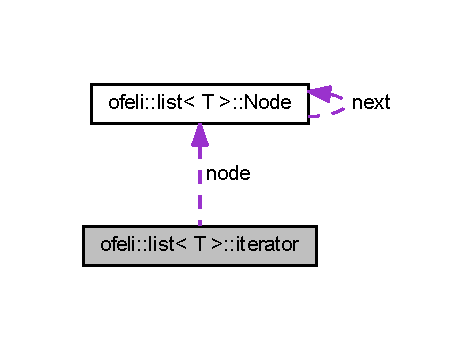
\includegraphics[width=228pt]{classofeli_1_1list_1_1iterator__coll__graph}
\end{center}
\end{figure}
\subsection*{Public Member Functions}
\begin{DoxyCompactItemize}
\item 
\hypertarget{classofeli_1_1list_1_1iterator_a4a8d4e7e15187464c623be990bf3d962}{T \& \hyperlink{classofeli_1_1list_1_1iterator_a4a8d4e7e15187464c623be990bf3d962}{operator$\ast$} () const }\label{classofeli_1_1list_1_1iterator_a4a8d4e7e15187464c623be990bf3d962}

\begin{DoxyCompactList}\small\item\em Gets the node data. {\itshape iterator} does not protect the data against writing. \end{DoxyCompactList}\item 
\hypertarget{classofeli_1_1list_1_1iterator_a687a367e3b5b94b3055e56f59b960567}{bool \hyperlink{classofeli_1_1list_1_1iterator_a687a367e3b5b94b3055e56f59b960567}{end} () const }\label{classofeli_1_1list_1_1iterator_a687a367e3b5b94b3055e56f59b960567}

\begin{DoxyCompactList}\small\item\em Checks if the iterator is at the end of the list, i.\-e. if the node is the sentinel node. \end{DoxyCompactList}\item 
\hypertarget{classofeli_1_1list_1_1iterator_a9c99a73cccabc3dd1325e1c243aca667}{\hyperlink{classofeli_1_1list_1_1iterator}{iterator} \& \hyperlink{classofeli_1_1list_1_1iterator_a9c99a73cccabc3dd1325e1c243aca667}{operator++} ()}\label{classofeli_1_1list_1_1iterator_a9c99a73cccabc3dd1325e1c243aca667}

\begin{DoxyCompactList}\small\item\em Increment the iterator. \end{DoxyCompactList}\end{DoxyCompactItemize}
\subsection*{Private Member Functions}
\begin{DoxyCompactItemize}
\item 
\hypertarget{classofeli_1_1list_1_1iterator_ac45584122cd0b4f60d046503595736b1}{\hyperlink{classofeli_1_1list_1_1iterator_ac45584122cd0b4f60d046503595736b1}{iterator} (\hyperlink{classofeli_1_1list_a7765ecb875543506d04dbd466f754503}{Link} node1)}\label{classofeli_1_1list_1_1iterator_ac45584122cd0b4f60d046503595736b1}

\begin{DoxyCompactList}\small\item\em Constructor with a node. \end{DoxyCompactList}\end{DoxyCompactItemize}
\subsection*{Private Attributes}
\begin{DoxyCompactItemize}
\item 
\hypertarget{classofeli_1_1list_1_1iterator_a6be3588fe536436d8c35c7db94beeb08}{\hyperlink{classofeli_1_1list_a7765ecb875543506d04dbd466f754503}{Link} \hyperlink{classofeli_1_1list_1_1iterator_a6be3588fe536436d8c35c7db94beeb08}{node}}\label{classofeli_1_1list_1_1iterator_a6be3588fe536436d8c35c7db94beeb08}

\begin{DoxyCompactList}\small\item\em {\itshape \hyperlink{classofeli_1_1list_1_1const__iterator}{const\-\_\-iterator}} encapsulates a pointer to a node. \end{DoxyCompactList}\end{DoxyCompactItemize}
\subsection*{Friends}
\begin{DoxyCompactItemize}
\item 
\hypertarget{classofeli_1_1list_1_1iterator_a39e8296e3b93358d0af90000b5d9113c}{class \hyperlink{classofeli_1_1list_1_1iterator_a39e8296e3b93358d0af90000b5d9113c}{list}}\label{classofeli_1_1list_1_1iterator_a39e8296e3b93358d0af90000b5d9113c}

\begin{DoxyCompactList}\small\item\em {\itshape list} has access to the private members of iterator. \end{DoxyCompactList}\end{DoxyCompactItemize}


\subsection{Detailed Description}
\subsubsection*{template$<$typename T = int$>$class ofeli\-::list$<$ T $>$\-::iterator}

Iterator to modify a list. 

Definition at line 119 of file linked\-\_\-list.\-hpp.



The documentation for this class was generated from the following file\-:\begin{DoxyCompactItemize}
\item 
linked\-\_\-list.\-hpp\end{DoxyCompactItemize}

\hypertarget{structofeli_1_1less}{\section{ofeli\-:\-:less$<$ T $>$ Struct Template Reference}
\label{structofeli_1_1less}\index{ofeli\-::less$<$ T $>$@{ofeli\-::less$<$ T $>$}}
}


{\ttfamily \#include $<$linked\-\_\-list.\-hpp$>$}

\subsection*{Public Member Functions}
\begin{DoxyCompactItemize}
\item 
\hypertarget{structofeli_1_1less_a4afc25c0817a8118a6222052c45bd597}{bool {\bfseries operator()} (const T \&x, const T \&y) const }\label{structofeli_1_1less_a4afc25c0817a8118a6222052c45bd597}

\end{DoxyCompactItemize}


\subsection{Detailed Description}
\subsubsection*{template$<$typename T = int$>$struct ofeli\-::less$<$ T $>$}

This class defines function objects for the \char`\"{}less than\char`\"{} inequality comparison operation. Generically, function objects are instances of a class with member function {\ttfamily operator()} defined. This member function allows the object to be used with the same syntax as a regular function call, and therefore it can be used in templates instead of a pointer to a function. {\ttfamily less} has its {\ttfamily operator()} member defined such that it returns {\ttfamily true} if its first argument compares lower than the second one using {\ttfamily operator$<$}, and {\ttfamily false} otherwise. This class can be used with the template function {\ttfamily \hyperlink{classofeli_1_1list_aaeedac18b70d233644d84c7ad3a9a3fa}{list$<$\-T$>$\-::sort(\-Binary\-Predicate compare)}}. 

Definition at line 385 of file linked\-\_\-list.\-hpp.



The documentation for this struct was generated from the following file\-:\begin{DoxyCompactItemize}
\item 
linked\-\_\-list.\-hpp\end{DoxyCompactItemize}

\hypertarget{structofeli_1_1less__equal}{\section{ofeli\-:\-:less\-\_\-equal$<$ T $>$ Struct Template Reference}
\label{structofeli_1_1less__equal}\index{ofeli\-::less\-\_\-equal$<$ T $>$@{ofeli\-::less\-\_\-equal$<$ T $>$}}
}


{\ttfamily \#include $<$linked\-\_\-list.\-hpp$>$}

\subsection*{Public Member Functions}
\begin{DoxyCompactItemize}
\item 
\hypertarget{structofeli_1_1less__equal_a8691d82bcc8b0cb6aa5e06ebc47d1a1d}{bool {\bfseries operator()} (const T \&x, const T \&y) const }\label{structofeli_1_1less__equal_a8691d82bcc8b0cb6aa5e06ebc47d1a1d}

\end{DoxyCompactItemize}


\subsection{Detailed Description}
\subsubsection*{template$<$typename T = int$>$struct ofeli\-::less\-\_\-equal$<$ T $>$}

This class defines function objects for the \char`\"{}less than or equal to\char`\"{} comparison operation ($<$=). Generically, function objects are instances of a class with member function {\ttfamily operator()} defined. This member function allows the object to be used with the same syntax as a regular function call, and therefore it can be used in templates instead of a pointer to a function. {\ttfamily \hyperlink{structofeli_1_1less__equal}{less\-\_\-equal}} has its {\ttfamily operator()} member defined such that it returns {\ttfamily true} if its first argument compares lower than or equal to the second one using {\ttfamily operator$<$=}, and {\ttfamily false} otherwise. This class can be used with the template function {\ttfamily \hyperlink{classofeli_1_1list_aaeedac18b70d233644d84c7ad3a9a3fa}{list$<$\-T$>$\-::sort(\-Binary\-Predicate compare)}}. 

Definition at line 391 of file linked\-\_\-list.\-hpp.



The documentation for this struct was generated from the following file\-:\begin{DoxyCompactItemize}
\item 
linked\-\_\-list.\-hpp\end{DoxyCompactItemize}

\hypertarget{classofeli_1_1list}{\section{ofeli\-:\-:list$<$ T $>$ Class Template Reference}
\label{classofeli_1_1list}\index{ofeli\-::list$<$ T $>$@{ofeli\-::list$<$ T $>$}}
}


{\ttfamily \#include $<$linked\-\_\-list.\-hpp$>$}



Collaboration diagram for ofeli\-:\-:list$<$ T $>$\-:\nopagebreak
\begin{figure}[H]
\begin{center}
\leavevmode
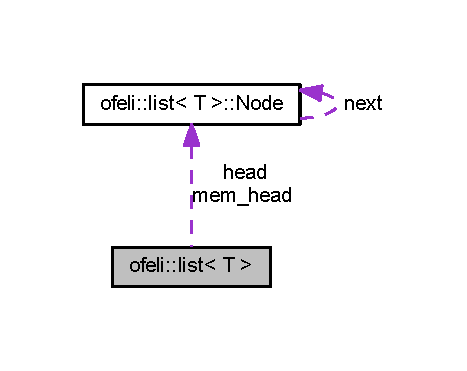
\includegraphics[width=224pt]{classofeli_1_1list__coll__graph}
\end{center}
\end{figure}
\subsection*{Classes}
\begin{DoxyCompactItemize}
\item 
class \hyperlink{classofeli_1_1list_1_1const__iterator}{const\-\_\-iterator}
\begin{DoxyCompactList}\small\item\em const iterator to read a const list. \end{DoxyCompactList}\item 
class \hyperlink{classofeli_1_1list_1_1iterator}{iterator}
\begin{DoxyCompactList}\small\item\em Iterator to modify a list. \end{DoxyCompactList}\item 
struct \hyperlink{structofeli_1_1list_1_1_node}{Node}
\begin{DoxyCompactList}\small\item\em This structure implements a node of class {\itshape list}. It is composed by an element of type {\itshape T} and a pointer on the next node. \end{DoxyCompactList}\end{DoxyCompactItemize}
\subsection*{Public Member Functions}
\begin{DoxyCompactItemize}
\item 
\hypertarget{classofeli_1_1list_a39932b3048b4ddbac43b00e7bad6a9da}{\hyperlink{classofeli_1_1list_a39932b3048b4ddbac43b00e7bad6a9da}{list} (int mem\-\_\-pool\-\_\-size1)}\label{classofeli_1_1list_a39932b3048b4ddbac43b00e7bad6a9da}

\begin{DoxyCompactList}\small\item\em Constructor. \end{DoxyCompactList}\item 
\hypertarget{classofeli_1_1list_add13c528e17c77a568aea94adec5db71}{\hyperlink{classofeli_1_1list_add13c528e17c77a568aea94adec5db71}{list} (int mem\-\_\-pool\-\_\-size1, int n, const T \&value)}\label{classofeli_1_1list_add13c528e17c77a568aea94adec5db71}

\begin{DoxyCompactList}\small\item\em Constructor to create a list with {\itshape n} value. \end{DoxyCompactList}\item 
\hypertarget{classofeli_1_1list_ac02bf0a0e738893734778313def2b557}{\hyperlink{classofeli_1_1list_ac02bf0a0e738893734778313def2b557}{list} (int mem\-\_\-pool\-\_\-size1, const T array\mbox{[}$\,$\mbox{]}, int array\-\_\-length)}\label{classofeli_1_1list_ac02bf0a0e738893734778313def2b557}

\begin{DoxyCompactList}\small\item\em Constructor to create a list from an array. \end{DoxyCompactList}\item 
\hypertarget{classofeli_1_1list_a6634b04ef70d4a4a11af6974e0b2b685}{\hyperlink{classofeli_1_1list_a6634b04ef70d4a4a11af6974e0b2b685}{list} (int mem\-\_\-pool\-\_\-size1, const \hyperlink{classofeli_1_1list}{list} \&copied)}\label{classofeli_1_1list_a6634b04ef70d4a4a11af6974e0b2b685}

\begin{DoxyCompactList}\small\item\em Copy constructor. \end{DoxyCompactList}\item 
\hypertarget{classofeli_1_1list_a0093d68c35e21c0b52c12a371be58826}{\hyperlink{classofeli_1_1list}{list} \& \hyperlink{classofeli_1_1list_a0093d68c35e21c0b52c12a371be58826}{operator=} (const \hyperlink{classofeli_1_1list}{list} \&rhs)}\label{classofeli_1_1list_a0093d68c35e21c0b52c12a371be58826}

\begin{DoxyCompactList}\small\item\em Assignment operator overloading. \end{DoxyCompactList}\item 
\hypertarget{classofeli_1_1list_a68fef2e0c33ffa015c2d4e9e8f11356a}{\hyperlink{classofeli_1_1list_a68fef2e0c33ffa015c2d4e9e8f11356a}{$\sim$list} ()}\label{classofeli_1_1list_a68fef2e0c33ffa015c2d4e9e8f11356a}

\begin{DoxyCompactList}\small\item\em Destructor. All the elements in the list container are dropped (including the sentinel node) \-: their destructors are called, and then they are removed from the list container, leaving it with a size of 0. \end{DoxyCompactList}\item 
\hypertarget{classofeli_1_1list_a1b4ab444619f6d412a461752ba019514}{void \hyperlink{classofeli_1_1list_a1b4ab444619f6d412a461752ba019514}{clear} ()}\label{classofeli_1_1list_a1b4ab444619f6d412a461752ba019514}

\begin{DoxyCompactList}\small\item\em All the elements in the list container are dropped (except the sentinel node) \-: their destructors are called, and then they are removed from the list container, leaving it with a size of 0. \end{DoxyCompactList}\item 
\hypertarget{classofeli_1_1list_a4f7f0567a64758636e3835ecea28a36f}{\hyperlink{classofeli_1_1list_1_1iterator}{iterator} \hyperlink{classofeli_1_1list_a4f7f0567a64758636e3835ecea28a36f}{begin} ()}\label{classofeli_1_1list_a4f7f0567a64758636e3835ecea28a36f}

\begin{DoxyCompactList}\small\item\em Returns the head link. \end{DoxyCompactList}\item 
\hypertarget{classofeli_1_1list_a2abcaf1bc66a9c292018efa55d6250ff}{\hyperlink{classofeli_1_1list_1_1const__iterator}{const\-\_\-iterator} \hyperlink{classofeli_1_1list_a2abcaf1bc66a9c292018efa55d6250ff}{begin} () const }\label{classofeli_1_1list_a2abcaf1bc66a9c292018efa55d6250ff}

\begin{DoxyCompactList}\small\item\em Returns the head link. \end{DoxyCompactList}\item 
void \hyperlink{classofeli_1_1list_a8c619ab7fedd643db5f3894889d91c74}{assign} (int n, const T \&value)
\item 
void \hyperlink{classofeli_1_1list_a7fbe8cc25a5c413924db708e47161306}{assign} (const T array\mbox{[}$\,$\mbox{]}, int array\-\_\-length)
\item 
\hypertarget{classofeli_1_1list_a38beb590b14408cbe2e0e5d573fbf5e2}{void \hyperlink{classofeli_1_1list_a38beb590b14408cbe2e0e5d573fbf5e2}{pop\-\_\-front} ()}\label{classofeli_1_1list_a38beb590b14408cbe2e0e5d573fbf5e2}

\begin{DoxyCompactList}\small\item\em Removes the first element in the {\itshape list} container, effectively reducing its size by one. \end{DoxyCompactList}\item 
\hypertarget{classofeli_1_1list_a87b7f6a90670e08d99e23f3377b001f9}{void \hyperlink{classofeli_1_1list_a87b7f6a90670e08d99e23f3377b001f9}{push\-\_\-front} (const T \&value)}\label{classofeli_1_1list_a87b7f6a90670e08d99e23f3377b001f9}

\begin{DoxyCompactList}\small\item\em Inserts a new element at the beginning of the list. \end{DoxyCompactList}\item 
\hypertarget{classofeli_1_1list_a05ae0af886d7932bdf5a5183e2a64c91}{void \hyperlink{classofeli_1_1list_a05ae0af886d7932bdf5a5183e2a64c91}{push\-\_\-front} (const \hyperlink{classofeli_1_1list}{list} \&copied)}\label{classofeli_1_1list_a05ae0af886d7932bdf5a5183e2a64c91}

\begin{DoxyCompactList}\small\item\em Inserts copies of list {\itshape copied} elements at the beginning of the list {\itshape $\ast$this}. \end{DoxyCompactList}\item 
\hypertarget{classofeli_1_1list_a3925aa31728a510af35d3229cd00a43f}{{\footnotesize template$<$typename Binary\-Predicate $>$ }\\void \hyperlink{classofeli_1_1list_a3925aa31728a510af35d3229cd00a43f}{put\-\_\-away} (const T \&value, Binary\-Predicate compare)}\label{classofeli_1_1list_a3925aa31728a510af35d3229cd00a43f}

\begin{DoxyCompactList}\small\item\em Puts away a new element to maintain sorted list into the specified order. \end{DoxyCompactList}\item 
\hypertarget{classofeli_1_1list_a0970694ba9e35222daa2ecc156f71661}{void \hyperlink{classofeli_1_1list_a0970694ba9e35222daa2ecc156f71661}{put\-\_\-away} (const T \&value)}\label{classofeli_1_1list_a0970694ba9e35222daa2ecc156f71661}

\begin{DoxyCompactList}\small\item\em Puts away a new element to maintain sorted list into ascending order. \end{DoxyCompactList}\item 
\hypertarget{classofeli_1_1list_a347778b1ef2f0530cb73403665f28caf}{\hyperlink{classofeli_1_1list_1_1iterator}{iterator} \hyperlink{classofeli_1_1list_a347778b1ef2f0530cb73403665f28caf}{insert\-\_\-before} (\hyperlink{classofeli_1_1list_1_1iterator}{iterator} position, const T \&value)}\label{classofeli_1_1list_a347778b1ef2f0530cb73403665f28caf}

\begin{DoxyCompactList}\small\item\em Inserts a new element before {\itshape position}. Returns the position of the inserted element. \end{DoxyCompactList}\item 
\hypertarget{classofeli_1_1list_a89cdc246b5f3b431d18e148d3dcad54e}{\hyperlink{classofeli_1_1list_1_1iterator}{iterator} \hyperlink{classofeli_1_1list_a89cdc246b5f3b431d18e148d3dcad54e}{insert\-\_\-after} (\hyperlink{classofeli_1_1list_1_1iterator}{iterator} position, const T \&value)}\label{classofeli_1_1list_a89cdc246b5f3b431d18e148d3dcad54e}

\begin{DoxyCompactList}\small\item\em Inserts a new element after {\itshape position}. Returns the position of the inserted element. \end{DoxyCompactList}\item 
\hypertarget{classofeli_1_1list_ae160d4ea7224becad437add3b1d594e4}{\hyperlink{classofeli_1_1list_1_1iterator}{iterator} \hyperlink{classofeli_1_1list_ae160d4ea7224becad437add3b1d594e4}{erase} (\hyperlink{classofeli_1_1list_1_1iterator}{iterator} position)}\label{classofeli_1_1list_ae160d4ea7224becad437add3b1d594e4}

\begin{DoxyCompactList}\small\item\em Removes from the list container the element at {\itshape position} and returns a valid iterator, i.\-e. the position of the next element. \end{DoxyCompactList}\item 
\hypertarget{classofeli_1_1list_a5f61ba4f2a9f7d67c4737baa9096386c}{\hyperlink{classofeli_1_1list_1_1iterator}{iterator} \hyperlink{classofeli_1_1list_a5f61ba4f2a9f7d67c4737baa9096386c}{erase\-\_\-after} (\hyperlink{classofeli_1_1list_1_1iterator}{iterator} position)}\label{classofeli_1_1list_a5f61ba4f2a9f7d67c4737baa9096386c}

\begin{DoxyCompactList}\small\item\em Removes from the list container the element at {\itshape ++position} and returns the position. \end{DoxyCompactList}\item 
\hyperlink{classofeli_1_1list_1_1iterator}{iterator} \hyperlink{classofeli_1_1list_af38ebb4b33ce7f5518b78eb1e8ae3464}{splice\-\_\-front} (\hyperlink{classofeli_1_1list_1_1iterator}{iterator} moved)
\item 
\hypertarget{classofeli_1_1list_a92338c30de397c0ac7bf224280c5607e}{void \hyperlink{classofeli_1_1list_a92338c30de397c0ac7bf224280c5607e}{splice\-\_\-front} (\hyperlink{classofeli_1_1list}{list} \&moved)}\label{classofeli_1_1list_a92338c30de397c0ac7bf224280c5607e}

\begin{DoxyCompactList}\small\item\em Moves all elements of list {\itshape moved} to the beginnning of list {\itshape $\ast$this}. \end{DoxyCompactList}\item 
\hypertarget{classofeli_1_1list_a6e9d56b7ca0771d3a768b588239a29f3}{void \hyperlink{classofeli_1_1list_a6e9d56b7ca0771d3a768b588239a29f3}{remove} (const T \&value)}\label{classofeli_1_1list_a6e9d56b7ca0771d3a768b588239a29f3}

\begin{DoxyCompactList}\small\item\em Removes elements by their value. \end{DoxyCompactList}\item 
{\footnotesize template$<$typename Unary\-Predicate $>$ }\\void \hyperlink{classofeli_1_1list_a2982d8f3bf7593929fe6ea3a7ad03fc6}{remove\-\_\-if} (Unary\-Predicate predicate)
\item 
{\footnotesize template$<$typename Binary\-Predicate $>$ }\\void \hyperlink{classofeli_1_1list_a640cb310a5241b411436ff39577706b1}{unique} (Binary\-Predicate compare)
\item 
\hypertarget{classofeli_1_1list_abc2cd2b67b1e9aab234cfeb647870f96}{void \hyperlink{classofeli_1_1list_abc2cd2b67b1e9aab234cfeb647870f96}{unique} ()}\label{classofeli_1_1list_abc2cd2b67b1e9aab234cfeb647870f96}

\begin{DoxyCompactList}\small\item\em Remove consecutive duplicate values. \end{DoxyCompactList}\item 
\hypertarget{classofeli_1_1list_a3cd2eabfec966e211118a90ab9d0a5f5}{void \hyperlink{classofeli_1_1list_a3cd2eabfec966e211118a90ab9d0a5f5}{reverse} ()}\label{classofeli_1_1list_a3cd2eabfec966e211118a90ab9d0a5f5}

\begin{DoxyCompactList}\small\item\em Reverses the order of the elements in the {\itshape list} container. \end{DoxyCompactList}\item 
\hypertarget{classofeli_1_1list_aaeedac18b70d233644d84c7ad3a9a3fa}{{\footnotesize template$<$typename Binary\-Predicate $>$ }\\void \hyperlink{classofeli_1_1list_aaeedac18b70d233644d84c7ad3a9a3fa}{sort} (Binary\-Predicate compare)}\label{classofeli_1_1list_aaeedac18b70d233644d84c7ad3a9a3fa}

\begin{DoxyCompactList}\small\item\em Sorts the elements with a specified order. The order of equal elements is guaranteed to be preserved (stability). The sorting is performed by merge sort algorithm in {\itshape O(n log n)} in worst-\/case, where {\itshape n} is the size of the container. It does not require {\itshape O(n)} extra space. \end{DoxyCompactList}\item 
\hypertarget{classofeli_1_1list_a6b47643ddf2f9ceeb952fb6a8617daf9}{void \hyperlink{classofeli_1_1list_a6b47643ddf2f9ceeb952fb6a8617daf9}{sort} ()}\label{classofeli_1_1list_a6b47643ddf2f9ceeb952fb6a8617daf9}

\begin{DoxyCompactList}\small\item\em Sorts the elements into ascending order. Calls the function void \hyperlink{classofeli_1_1list_aaeedac18b70d233644d84c7ad3a9a3fa}{sort(\-Binary\-Predicate compare)} with an object of the class {\itshape less} because parameter by default for a template function is not allowed. \end{DoxyCompactList}\item 
\hypertarget{classofeli_1_1list_ab3e6e91f6df59f3bf1b290a36577e474}{bool \hyperlink{classofeli_1_1list_ab3e6e91f6df59f3bf1b290a36577e474}{empty} () const }\label{classofeli_1_1list_ab3e6e91f6df59f3bf1b290a36577e474}

\begin{DoxyCompactList}\small\item\em Returns whether the list container is empty, i.\-e. whether its size is 0. \end{DoxyCompactList}\item 
int \hyperlink{classofeli_1_1list_ab4901f65fa96e300ce11dc75e0760dda}{size} () const 
\item 
\hypertarget{classofeli_1_1list_ac904f35ef541477948b304f69cdc7384}{void \hyperlink{classofeli_1_1list_ac904f35ef541477948b304f69cdc7384}{display} () const }\label{classofeli_1_1list_ac904f35ef541477948b304f69cdc7384}

\begin{DoxyCompactList}\small\item\em A second way to display a linked list. \end{DoxyCompactList}\item 
\hypertarget{classofeli_1_1list_ad0f411dfb78ecfa34f66078a64f7ccb6}{T $\ast$ \hyperlink{classofeli_1_1list_ad0f411dfb78ecfa34f66078a64f7ccb6}{get\-\_\-array} (int array\-\_\-length) const }\label{classofeli_1_1list_ad0f411dfb78ecfa34f66078a64f7ccb6}

\begin{DoxyCompactList}\small\item\em Gets an array with the value of list {\itshape $\ast$this}. \end{DoxyCompactList}\end{DoxyCompactItemize}
\subsection*{Static Public Member Functions}
\begin{DoxyCompactItemize}
\item 
static void \hyperlink{classofeli_1_1list_a471424ff8c258a2c00e9246035304cff}{swap} (\hyperlink{classofeli_1_1list}{list} \&list1, \hyperlink{classofeli_1_1list}{list} \&list2)
\end{DoxyCompactItemize}
\subsection*{Private Types}
\begin{DoxyCompactItemize}
\item 
\hypertarget{classofeli_1_1list_a7765ecb875543506d04dbd466f754503}{typedef \hyperlink{structofeli_1_1list_1_1_node}{Node} $\ast$ \hyperlink{classofeli_1_1list_a7765ecb875543506d04dbd466f754503}{Link}}\label{classofeli_1_1list_a7765ecb875543506d04dbd466f754503}

\begin{DoxyCompactList}\small\item\em Link is a pointer to a \hyperlink{structofeli_1_1list_1_1_node}{Node}. \end{DoxyCompactList}\end{DoxyCompactItemize}
\subsection*{Private Member Functions}
\begin{DoxyCompactItemize}
\item 
\hypertarget{classofeli_1_1list_ac969c1209e5bd5b41a8e56e192061aea}{void \hyperlink{classofeli_1_1list_ac969c1209e5bd5b41a8e56e192061aea}{alloc\-\_\-mem\-\_\-pool} ()}\label{classofeli_1_1list_ac969c1209e5bd5b41a8e56e192061aea}

\begin{DoxyCompactList}\small\item\em Creates a memory pool with a shared linked list. \end{DoxyCompactList}\end{DoxyCompactItemize}
\subsection*{Private Attributes}
\begin{DoxyCompactItemize}
\item 
\hypertarget{classofeli_1_1list_aed33fb6086a95ce25dd474aef8063661}{\hyperlink{classofeli_1_1list_a7765ecb875543506d04dbd466f754503}{Link} \hyperlink{classofeli_1_1list_aed33fb6086a95ce25dd474aef8063661}{head}}\label{classofeli_1_1list_aed33fb6086a95ce25dd474aef8063661}

\begin{DoxyCompactList}\small\item\em Head of the list. \end{DoxyCompactList}\item 
\hypertarget{classofeli_1_1list_a4751e1b2279d0dcff01b0081d0dcbd19}{const int \hyperlink{classofeli_1_1list_a4751e1b2279d0dcff01b0081d0dcbd19}{mem\-\_\-pool\-\_\-size}}\label{classofeli_1_1list_a4751e1b2279d0dcff01b0081d0dcbd19}

\begin{DoxyCompactList}\small\item\em Number of nodes of the memory pool list created by list $\ast$this. \end{DoxyCompactList}\end{DoxyCompactItemize}
\subsection*{Static Private Attributes}
\begin{DoxyCompactItemize}
\item 
\hypertarget{classofeli_1_1list_a8a313f391f6672c8c26ab5d9c7f58396}{static \hyperlink{classofeli_1_1list_a7765ecb875543506d04dbd466f754503}{Link} \hyperlink{classofeli_1_1list_a8a313f391f6672c8c26ab5d9c7f58396}{mem\-\_\-head}}\label{classofeli_1_1list_a8a313f391f6672c8c26ab5d9c7f58396}

\begin{DoxyCompactList}\small\item\em Head of the memory pool list which is shared for all lists. \end{DoxyCompactList}\end{DoxyCompactItemize}
\subsection*{Friends}
\begin{DoxyCompactItemize}
\item 
\hypertarget{classofeli_1_1list_a4ad2e66a0acf1d35b209f40c861aeae8}{{\footnotesize template$<$class U $>$ }\\bool \hyperlink{classofeli_1_1list_a4ad2e66a0acf1d35b209f40c861aeae8}{operator==} (const \hyperlink{classofeli_1_1list}{list}$<$ U $>$ \&lhs, const \hyperlink{classofeli_1_1list}{list}$<$ U $>$ \&rhs)}\label{classofeli_1_1list_a4ad2e66a0acf1d35b209f40c861aeae8}

\begin{DoxyCompactList}\small\item\em {\itshape Equal} {\itshape to} operator overloading. \end{DoxyCompactList}\item 
\hypertarget{classofeli_1_1list_a5f0cc9d1a3a2bcb2450cec7eb0f2dcb6}{{\footnotesize template$<$class U $>$ }\\bool \hyperlink{classofeli_1_1list_a5f0cc9d1a3a2bcb2450cec7eb0f2dcb6}{operator!=} (const \hyperlink{classofeli_1_1list}{list}$<$ U $>$ \&lhs, const \hyperlink{classofeli_1_1list}{list}$<$ U $>$ \&rhs)}\label{classofeli_1_1list_a5f0cc9d1a3a2bcb2450cec7eb0f2dcb6}

\begin{DoxyCompactList}\small\item\em {\itshape Not} {\itshape equal} {\itshape to} operator overloading. \end{DoxyCompactList}\item 
\hypertarget{classofeli_1_1list_ab34eccc5c4d4d114a5f6654becd48c9c}{{\footnotesize template$<$class U $>$ }\\std\-::ostream \& \hyperlink{classofeli_1_1list_ab34eccc5c4d4d114a5f6654becd48c9c}{operator$<$$<$} (std\-::ostream \&os, const \hyperlink{classofeli_1_1list}{list}$<$ U $>$ \&displayed)}\label{classofeli_1_1list_ab34eccc5c4d4d114a5f6654becd48c9c}

\begin{DoxyCompactList}\small\item\em Overloading of cout $<$$<$. It displays a linked list in the same way as integral-\/type variable. \end{DoxyCompactList}\end{DoxyCompactItemize}


\subsection{Detailed Description}
\subsubsection*{template$<$typename T = int$>$class ofeli\-::list$<$ T $>$}

This class implements a singly linked list used by the implementation of Shi and Karl' algorithm. The elements stored are integers by default that correspond of the offset of the level set function buffer. 

Definition at line 50 of file linked\-\_\-list.\-hpp.



\subsection{Member Function Documentation}
\hypertarget{classofeli_1_1list_a8c619ab7fedd643db5f3894889d91c74}{\index{ofeli\-::list@{ofeli\-::list}!assign@{assign}}
\index{assign@{assign}!ofeli::list@{ofeli\-::list}}
\subsubsection[{assign}]{\setlength{\rightskip}{0pt plus 5cm}template$<$typename T = int$>$ void {\bf ofeli\-::list}$<$ T $>$\-::assign (
\begin{DoxyParamCaption}
\item[{int}]{n, }
\item[{const T \&}]{value}
\end{DoxyParamCaption}
)}}\label{classofeli_1_1list_a8c619ab7fedd643db5f3894889d91c74}
Assigns new content to the container, dropping all the elements contained in the container object before the call and replacing them by those specified by the parameters\-:
\begin{DoxyItemize}
\item the new content is the repetition {\itshape n} times of copies of element value. 
\end{DoxyItemize}\hypertarget{classofeli_1_1list_a7fbe8cc25a5c413924db708e47161306}{\index{ofeli\-::list@{ofeli\-::list}!assign@{assign}}
\index{assign@{assign}!ofeli::list@{ofeli\-::list}}
\subsubsection[{assign}]{\setlength{\rightskip}{0pt plus 5cm}template$<$typename T = int$>$ void {\bf ofeli\-::list}$<$ T $>$\-::assign (
\begin{DoxyParamCaption}
\item[{const T}]{array\mbox{[}$\,$\mbox{]}, }
\item[{int}]{array\-\_\-length}
\end{DoxyParamCaption}
)}}\label{classofeli_1_1list_a7fbe8cc25a5c413924db708e47161306}
Assigns new content to the container, dropping all the elements contained in the container object before the call and replacing them by those specified by the parameters\-:
\begin{DoxyItemize}
\item the new content is a copy of an array. 
\end{DoxyItemize}\hypertarget{classofeli_1_1list_a2982d8f3bf7593929fe6ea3a7ad03fc6}{\index{ofeli\-::list@{ofeli\-::list}!remove\-\_\-if@{remove\-\_\-if}}
\index{remove\-\_\-if@{remove\-\_\-if}!ofeli::list@{ofeli\-::list}}
\subsubsection[{remove\-\_\-if}]{\setlength{\rightskip}{0pt plus 5cm}template$<$typename T = int$>$ template$<$typename Unary\-Predicate $>$ void {\bf ofeli\-::list}$<$ T $>$\-::remove\-\_\-if (
\begin{DoxyParamCaption}
\item[{Unary\-Predicate}]{predicate}
\end{DoxyParamCaption}
)}}\label{classofeli_1_1list_a2982d8f3bf7593929fe6ea3a7ad03fc6}
Removes from the container all the elements for which {\itshape Predicate} {\itshape predicate} returns {\ttfamily true}. This calls the destructor of these objects and reduces the container size by the number of elements removed. Unary\-Predicate {\itshape predicate} can be implemented as any typed expression taking one argument of the same type as the elements container in the {\itshape list} and returning a bool (this may either be a function pointer or an object whose class implements {\ttfamily operator()}). \hypertarget{classofeli_1_1list_ab4901f65fa96e300ce11dc75e0760dda}{\index{ofeli\-::list@{ofeli\-::list}!size@{size}}
\index{size@{size}!ofeli::list@{ofeli\-::list}}
\subsubsection[{size}]{\setlength{\rightskip}{0pt plus 5cm}template$<$typename T = int$>$ int {\bf ofeli\-::list}$<$ T $>$\-::size (
\begin{DoxyParamCaption}
{}
\end{DoxyParamCaption}
) const}}\label{classofeli_1_1list_ab4901f65fa96e300ce11dc75e0760dda}
Returns the number of elements in the list without counting the sentinel node. The complexity of this function is in {\itshape O(n)} so if you want to get often the size of the list, you should update the size in a variable after each modification. \hypertarget{classofeli_1_1list_af38ebb4b33ce7f5518b78eb1e8ae3464}{\index{ofeli\-::list@{ofeli\-::list}!splice\-\_\-front@{splice\-\_\-front}}
\index{splice\-\_\-front@{splice\-\_\-front}!ofeli::list@{ofeli\-::list}}
\subsubsection[{splice\-\_\-front}]{\setlength{\rightskip}{0pt plus 5cm}template$<$typename T = int$>$ {\bf iterator} {\bf ofeli\-::list}$<$ T $>$\-::splice\-\_\-front (
\begin{DoxyParamCaption}
\item[{{\bf iterator}}]{moved}
\end{DoxyParamCaption}
)}}\label{classofeli_1_1list_af38ebb4b33ce7f5518b78eb1e8ae3464}
Removes an element {\itshape moved} (of another list or list {\itshape $\ast$this}) and inserts at the beginning of list {\itshape $\ast$this}. Equivalent to push\-\_\-front($\ast$it) and it = erase(it) without use of the operators {\itshape new} and {\itshape delete}. Returns a valid iterator, i.\-e the position of the next element. 

Here is the caller graph for this function\-:\nopagebreak
\begin{figure}[H]
\begin{center}
\leavevmode
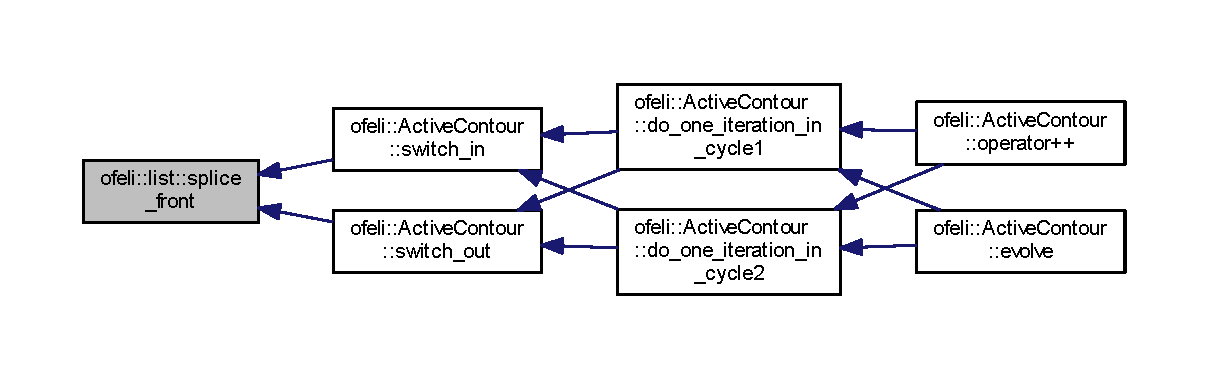
\includegraphics[width=350pt]{classofeli_1_1list_af38ebb4b33ce7f5518b78eb1e8ae3464_icgraph}
\end{center}
\end{figure}


\hypertarget{classofeli_1_1list_a471424ff8c258a2c00e9246035304cff}{\index{ofeli\-::list@{ofeli\-::list}!swap@{swap}}
\index{swap@{swap}!ofeli::list@{ofeli\-::list}}
\subsubsection[{swap}]{\setlength{\rightskip}{0pt plus 5cm}template$<$typename T = int$>$ static void {\bf ofeli\-::list}$<$ T $>$\-::swap (
\begin{DoxyParamCaption}
\item[{{\bf list}$<$ T $>$ \&}]{list1, }
\item[{{\bf list}$<$ T $>$ \&}]{list2}
\end{DoxyParamCaption}
)\hspace{0.3cm}{\ttfamily [static]}}}\label{classofeli_1_1list_a471424ff8c258a2c00e9246035304cff}
Exchanges the content of container {\itshape list1} by the content of {\itshape list2}, which is another list object containing elements of the same type. Sizes may differ. Performs it in a constant time without copying. Use this function if you don't have accesss to C++11 (formerly known as C++0x) \char`\"{}void std\-::swap(\-T\& a, T\& b)\char`\"{} version with semantic move. \hypertarget{classofeli_1_1list_a640cb310a5241b411436ff39577706b1}{\index{ofeli\-::list@{ofeli\-::list}!unique@{unique}}
\index{unique@{unique}!ofeli::list@{ofeli\-::list}}
\subsubsection[{unique}]{\setlength{\rightskip}{0pt plus 5cm}template$<$typename T = int$>$ template$<$typename Binary\-Predicate $>$ void {\bf ofeli\-::list}$<$ T $>$\-::unique (
\begin{DoxyParamCaption}
\item[{Binary\-Predicate}]{compare}
\end{DoxyParamCaption}
)}}\label{classofeli_1_1list_a640cb310a5241b411436ff39577706b1}
This version accepting a binary predicate, a specific comparison function to determine the \char`\"{}uniqueness\char`\"{} of an element can be specified. In fact, any behavior can be implemented (and not only an equality comparison), but notice that the function will call binary\-\_\-pred({\itshape i,}(i-\/1)) for all pairs of elements (where i is an iterator to an element, starting from the second) and remove i from the list if the predicate returns {\ttfamily true}. 

The documentation for this class was generated from the following file\-:\begin{DoxyCompactItemize}
\item 
linked\-\_\-list.\-hpp\end{DoxyCompactItemize}

\hypertarget{classlist}{\section{list$<$ T $>$ Class Template Reference}
\label{classlist}\index{list$<$ T $>$@{list$<$ T $>$}}
}


\subsection{Detailed Description}
\subsubsection*{template$<$typename T$>$class list$<$ T $>$}

\begin{Desc}
\item[Examples\-: ]\par
\hyperlink{linked_list-example}{linked\-\_\-list}.\end{Desc}


Definition at line 64 of file imageviewer.\-hpp.



The documentation for this class was generated from the following file\-:\begin{DoxyCompactItemize}
\item 
imageviewer.\-hpp\end{DoxyCompactItemize}

\hypertarget{structofeli_1_1list_1_1_node}{\section{ofeli\-:\-:list$<$ T $>$\-:\-:Node Struct Reference}
\label{structofeli_1_1list_1_1_node}\index{ofeli\-::list$<$ T $>$\-::\-Node@{ofeli\-::list$<$ T $>$\-::\-Node}}
}


This structure implements a node of class {\itshape list}. It is composed by an element of type {\itshape T} and a pointer on the next node.  




Collaboration diagram for ofeli\-:\-:list$<$ T $>$\-:\-:Node\-:\nopagebreak
\begin{figure}[H]
\begin{center}
\leavevmode
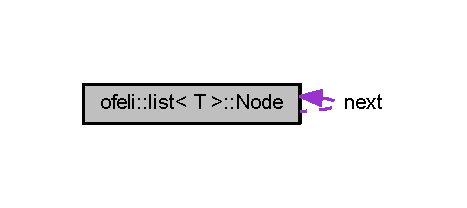
\includegraphics[width=224pt]{structofeli_1_1list_1_1_node__coll__graph}
\end{center}
\end{figure}
\subsection*{Public Member Functions}
\begin{DoxyCompactItemize}
\item 
\hypertarget{structofeli_1_1list_1_1_node_aa51604521fb273117e7008fb2ebd2949}{\hyperlink{structofeli_1_1list_1_1_node_aa51604521fb273117e7008fb2ebd2949}{Node} (const T \&data1, \hyperlink{classofeli_1_1list_a7765ecb875543506d04dbd466f754503}{Link} next1)}\label{structofeli_1_1list_1_1_node_aa51604521fb273117e7008fb2ebd2949}

\begin{DoxyCompactList}\small\item\em Constructor. \end{DoxyCompactList}\item 
\hypertarget{structofeli_1_1list_1_1_node_a0dec619f483d887884d5fcd963e65d9b}{bool \hyperlink{structofeli_1_1list_1_1_node_a0dec619f483d887884d5fcd963e65d9b}{end} () const }\label{structofeli_1_1list_1_1_node_a0dec619f483d887884d5fcd963e65d9b}

\begin{DoxyCompactList}\small\item\em Checks if the node is at the end of the list, i.\-e. if the node is the sentinel node. \end{DoxyCompactList}\end{DoxyCompactItemize}
\subsection*{Static Public Member Functions}
\begin{DoxyCompactItemize}
\item 
\hypertarget{structofeli_1_1list_1_1_node_ac75b630e0b50f5eee672e8a0a8aca132}{static \hyperlink{classofeli_1_1list_a7765ecb875543506d04dbd466f754503}{Link} \hyperlink{structofeli_1_1list_1_1_node_ac75b630e0b50f5eee672e8a0a8aca132}{new\-\_\-} (const T \&data1, \hyperlink{classofeli_1_1list_a7765ecb875543506d04dbd466f754503}{Link} next1)}\label{structofeli_1_1list_1_1_node_ac75b630e0b50f5eee672e8a0a8aca132}

\begin{DoxyCompactList}\small\item\em Collects a node from the linked list memory pool and initializes it. It mimes operator {\ttfamily new}. \end{DoxyCompactList}\item 
\hypertarget{structofeli_1_1list_1_1_node_a6b9d48c85eee2608978fe420d03b3e73}{static \hyperlink{classofeli_1_1list_a7765ecb875543506d04dbd466f754503}{Link} \hyperlink{structofeli_1_1list_1_1_node_a6b9d48c85eee2608978fe420d03b3e73}{new\-\_\-} (const \hyperlink{structofeli_1_1list_1_1_node}{Node} \&copied)}\label{structofeli_1_1list_1_1_node_a6b9d48c85eee2608978fe420d03b3e73}

\begin{DoxyCompactList}\small\item\em Collects a node from the linked list memory pool and initializes it. It mimes operator {\ttfamily new}. \end{DoxyCompactList}\item 
\hypertarget{structofeli_1_1list_1_1_node_a42cedc598273b73b0f2bc34f7cd10043}{static void \hyperlink{structofeli_1_1list_1_1_node_a42cedc598273b73b0f2bc34f7cd10043}{delete\-\_\-} (\hyperlink{classofeli_1_1list_a7765ecb875543506d04dbd466f754503}{Link} node)}\label{structofeli_1_1list_1_1_node_a42cedc598273b73b0f2bc34f7cd10043}

\begin{DoxyCompactList}\small\item\em Moves a node to the linked list memory pool. It mimes operator {\ttfamily delete}. \end{DoxyCompactList}\end{DoxyCompactItemize}
\subsection*{Public Attributes}
\begin{DoxyCompactItemize}
\item 
\hypertarget{structofeli_1_1list_1_1_node_a50e84fcefcfc088b1beb4db228da2665}{T \hyperlink{structofeli_1_1list_1_1_node_a50e84fcefcfc088b1beb4db228da2665}{data}}\label{structofeli_1_1list_1_1_node_a50e84fcefcfc088b1beb4db228da2665}

\begin{DoxyCompactList}\small\item\em Element storage. \end{DoxyCompactList}\item 
\hypertarget{structofeli_1_1list_1_1_node_a6c04294f1a7e9fe11737c4e041e93f03}{\hyperlink{classofeli_1_1list_a7765ecb875543506d04dbd466f754503}{Link} \hyperlink{structofeli_1_1list_1_1_node_a6c04294f1a7e9fe11737c4e041e93f03}{next}}\label{structofeli_1_1list_1_1_node_a6c04294f1a7e9fe11737c4e041e93f03}

\begin{DoxyCompactList}\small\item\em Pointer to the next node. \end{DoxyCompactList}\end{DoxyCompactItemize}


\subsection{Detailed Description}
\subsubsection*{template$<$typename T = int$>$struct ofeli\-::list$<$ T $>$\-::\-Node}

This structure implements a node of class {\itshape list}. It is composed by an element of type {\itshape T} and a pointer on the next node. 

Definition at line 160 of file linked\-\_\-list.\-hpp.



The documentation for this struct was generated from the following file\-:\begin{DoxyCompactItemize}
\item 
linked\-\_\-list.\-hpp\end{DoxyCompactItemize}

\hypertarget{structofeli_1_1not__equal__to}{\section{ofeli\-:\-:not\-\_\-equal\-\_\-to$<$ T $>$ Struct Template Reference}
\label{structofeli_1_1not__equal__to}\index{ofeli\-::not\-\_\-equal\-\_\-to$<$ T $>$@{ofeli\-::not\-\_\-equal\-\_\-to$<$ T $>$}}
}


{\ttfamily \#include $<$linked\-\_\-list.\-hpp$>$}

\subsection*{Public Member Functions}
\begin{DoxyCompactItemize}
\item 
\hypertarget{structofeli_1_1not__equal__to_ac3562b5ed24603ab03e5acc462db9974}{bool {\bfseries operator()} (const T \&x, const T \&y) const }\label{structofeli_1_1not__equal__to_ac3562b5ed24603ab03e5acc462db9974}

\end{DoxyCompactItemize}


\subsection{Detailed Description}
\subsubsection*{template$<$typename T = int$>$struct ofeli\-::not\-\_\-equal\-\_\-to$<$ T $>$}

This class defines function objects for the non-\/equality comparison operation. Generically, function objects are instances of a class with member function {\ttfamily operator()} defined. This member function allows the object to be used with the same syntax as a regular function call, and therefore it can be used in templates instead of a pointer to a function. {\ttfamily \hyperlink{structofeli_1_1not__equal__to}{not\-\_\-equal\-\_\-to}} has its {\ttfamily operator()} member defined such that it returns {\ttfamily true} if its two arguments do not compare equal to each other using {\ttfamily operator!=}, and {\ttfamily false} otherwise. This class can be used with the template function {\ttfamily \hyperlink{classofeli_1_1list_aaeedac18b70d233644d84c7ad3a9a3fa}{list$<$\-T$>$\-::sort(\-Binary\-Predicate compare)}}. 

Definition at line 379 of file linked\-\_\-list.\-hpp.



The documentation for this struct was generated from the following file\-:\begin{DoxyCompactItemize}
\item 
linked\-\_\-list.\-hpp\end{DoxyCompactItemize}

\hypertarget{classofeli_1_1_pixmap_widget}{\section{ofeli\-:\-:Pixmap\-Widget Class Reference}
\label{classofeli_1_1_pixmap_widget}\index{ofeli\-::\-Pixmap\-Widget@{ofeli\-::\-Pixmap\-Widget}}
}


{\ttfamily \#include $<$pixmapwidget.\-hpp$>$}



Inheritance diagram for ofeli\-:\-:Pixmap\-Widget\-:\nopagebreak
\begin{figure}[H]
\begin{center}
\leavevmode
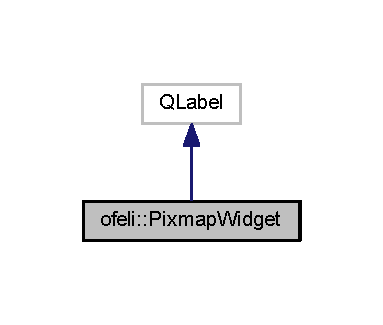
\includegraphics[width=184pt]{classofeli_1_1_pixmap_widget__inherit__graph}
\end{center}
\end{figure}


Collaboration diagram for ofeli\-:\-:Pixmap\-Widget\-:\nopagebreak
\begin{figure}[H]
\begin{center}
\leavevmode
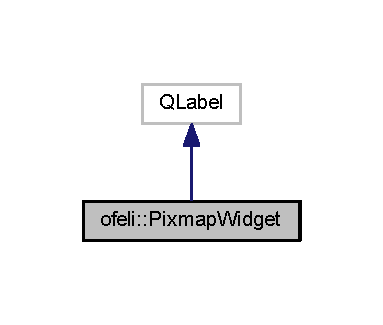
\includegraphics[width=184pt]{classofeli_1_1_pixmap_widget__coll__graph}
\end{center}
\end{figure}
\subsection*{Public Slots}
\begin{DoxyCompactItemize}
\item 
\hypertarget{classofeli_1_1_pixmap_widget_ae245448eabde60edd6d4543da56ae11b}{void {\bfseries set\-Zoom\-Factor} (float f)}\label{classofeli_1_1_pixmap_widget_ae245448eabde60edd6d4543da56ae11b}

\end{DoxyCompactItemize}
\subsection*{Signals}
\begin{DoxyCompactItemize}
\item 
\hypertarget{classofeli_1_1_pixmap_widget_ab817a81f26b323d58c0cf659912080d4}{void {\bfseries zoom\-Factor\-Changed} (float f)}\label{classofeli_1_1_pixmap_widget_ab817a81f26b323d58c0cf659912080d4}

\end{DoxyCompactItemize}
\subsection*{Public Member Functions}
\begin{DoxyCompactItemize}
\item 
\hypertarget{classofeli_1_1_pixmap_widget_a51fe3171285939f9fa39cb46afb505e0}{{\bfseries Pixmap\-Widget} (Q\-Widget $\ast$parent=0)}\label{classofeli_1_1_pixmap_widget_a51fe3171285939f9fa39cb46afb505e0}

\item 
\hypertarget{classofeli_1_1_pixmap_widget_a0169b3ce7c469ac8e809275cec1d6cdf}{void {\bfseries set\-\_\-qimage0} (const Q\-Image \&qimage1)}\label{classofeli_1_1_pixmap_widget_a0169b3ce7c469ac8e809275cec1d6cdf}

\item 
\hypertarget{classofeli_1_1_pixmap_widget_a553fb5a31a88e84ddf8490811cd8f6fe}{void {\bfseries set\-\_\-qimage} (const Q\-Image \&qimage1)}\label{classofeli_1_1_pixmap_widget_a553fb5a31a88e84ddf8490811cd8f6fe}

\item 
\hypertarget{classofeli_1_1_pixmap_widget_a16df598b66b7acca419e52172b1f91a7}{void {\bfseries set\-\_\-do\-Wheel\-Event} (bool do\-Wheel\-Event1)}\label{classofeli_1_1_pixmap_widget_a16df598b66b7acca419e52172b1f91a7}

\item 
\hypertarget{classofeli_1_1_pixmap_widget_ab051e68d52dad2be8636a48eab25da06}{void {\bfseries set\-\_\-zoom\-Factor} (float zoom\-Factor1)}\label{classofeli_1_1_pixmap_widget_ab051e68d52dad2be8636a48eab25da06}

\item 
\hypertarget{classofeli_1_1_pixmap_widget_a4484eb00d84068802f22735a8ed76e4c}{float {\bfseries get\-\_\-zoom\-Factor} () const }\label{classofeli_1_1_pixmap_widget_a4484eb00d84068802f22735a8ed76e4c}

\item 
\hypertarget{classofeli_1_1_pixmap_widget_aaa829326021c312a97374c1362f8d298}{int {\bfseries get\-Pix\-Width} () const }\label{classofeli_1_1_pixmap_widget_aaa829326021c312a97374c1362f8d298}

\item 
\hypertarget{classofeli_1_1_pixmap_widget_a978fbda49d780bb1444bd049aaf6e3fb}{int {\bfseries get\-Pix\-Height} () const }\label{classofeli_1_1_pixmap_widget_a978fbda49d780bb1444bd049aaf6e3fb}

\item 
\hypertarget{classofeli_1_1_pixmap_widget_a7e09147dfb98b3fb96e98d284b33fd71}{int {\bfseries get\-\_\-xoffset} () const }\label{classofeli_1_1_pixmap_widget_a7e09147dfb98b3fb96e98d284b33fd71}

\item 
\hypertarget{classofeli_1_1_pixmap_widget_a65b752a51f28973ef731cfd96ef1b726}{int {\bfseries get\-\_\-yoffset} () const }\label{classofeli_1_1_pixmap_widget_a65b752a51f28973ef731cfd96ef1b726}

\item 
\hypertarget{classofeli_1_1_pixmap_widget_a104e3d8592d5c6ed4bd06576e434d31b}{void {\bfseries set\-\_\-has\-Text} (bool has\-Text1)}\label{classofeli_1_1_pixmap_widget_a104e3d8592d5c6ed4bd06576e434d31b}

\item 
\hypertarget{classofeli_1_1_pixmap_widget_ab68827bf2b993a222b16e35a886f5b32}{const Q\-Image \& {\bfseries get\-\_\-qimage} () const }\label{classofeli_1_1_pixmap_widget_ab68827bf2b993a222b16e35a886f5b32}

\item 
\hypertarget{classofeli_1_1_pixmap_widget_ab98a6363c2b5bf9653fff1fa64e593d6}{void {\bfseries set\-\_\-text} (Q\-String text1)}\label{classofeli_1_1_pixmap_widget_ab98a6363c2b5bf9653fff1fa64e593d6}

\end{DoxyCompactItemize}
\subsection*{Protected Member Functions}
\begin{DoxyCompactItemize}
\item 
\hypertarget{classofeli_1_1_pixmap_widget_abd9c20f706e6d1ff8147ddb3a911e8f5}{void {\bfseries paint\-Event} (Q\-Paint\-Event $\ast$event)}\label{classofeli_1_1_pixmap_widget_abd9c20f706e6d1ff8147ddb3a911e8f5}

\item 
\hypertarget{classofeli_1_1_pixmap_widget_af12f9ad6114acba9f3907fe20577a2a9}{void {\bfseries wheel\-Event} (Q\-Wheel\-Event $\ast$event)}\label{classofeli_1_1_pixmap_widget_af12f9ad6114acba9f3907fe20577a2a9}

\end{DoxyCompactItemize}
\subsection*{Private Attributes}
\begin{DoxyCompactItemize}
\item 
\hypertarget{classofeli_1_1_pixmap_widget_aa9185a44438e16a0a423cb353f9ddacd}{Q\-Image {\bfseries qimage}}\label{classofeli_1_1_pixmap_widget_aa9185a44438e16a0a423cb353f9ddacd}

\item 
\hypertarget{classofeli_1_1_pixmap_widget_a621299723d4edde9cb4454ac4dfb3200}{float {\bfseries zoom\-Factor}}\label{classofeli_1_1_pixmap_widget_a621299723d4edde9cb4454ac4dfb3200}

\item 
\hypertarget{classofeli_1_1_pixmap_widget_adfedb996ccee157d87581a60af4dd278}{int {\bfseries xoffset}}\label{classofeli_1_1_pixmap_widget_adfedb996ccee157d87581a60af4dd278}

\item 
\hypertarget{classofeli_1_1_pixmap_widget_a7ca491af4dcb996a2af7eb9ae9f6a3ee}{int {\bfseries yoffset}}\label{classofeli_1_1_pixmap_widget_a7ca491af4dcb996a2af7eb9ae9f6a3ee}

\item 
\hypertarget{classofeli_1_1_pixmap_widget_a3da7d16f1a12fc64a85860ccb1f09598}{bool {\bfseries has\-Text}}\label{classofeli_1_1_pixmap_widget_a3da7d16f1a12fc64a85860ccb1f09598}

\item 
\hypertarget{classofeli_1_1_pixmap_widget_a1a75f2bd4da1f85d1e8ab3880dc76dbf}{Q\-String {\bfseries text}}\label{classofeli_1_1_pixmap_widget_a1a75f2bd4da1f85d1e8ab3880dc76dbf}

\item 
\hypertarget{classofeli_1_1_pixmap_widget_a9cbffb16d41dbaa2d0f6fc787c69966c}{bool {\bfseries do\-Wheel\-Event}}\label{classofeli_1_1_pixmap_widget_a9cbffb16d41dbaa2d0f6fc787c69966c}

\end{DoxyCompactItemize}


\subsection{Detailed Description}
The class \hyperlink{classofeli_1_1_pixmap_widget}{Pixmap\-Widget} is a Qt4 widget to display fastly an image (function draw\-Pixmap in a Paint\-Event is faster than function set\-Pixmap) and gives the possibility to zoom with a mouse wheel event in function of the position of the cursor. Thanks to Johan Thelin. This class is based on this example \href{http://qt4.digitalfanatics.org/articles/zoomer.html}{\tt http\-://qt4.\-digitalfanatics.\-org/articles/zoomer.\-html}. 

Definition at line 53 of file pixmapwidget.\-hpp.



The documentation for this class was generated from the following files\-:\begin{DoxyCompactItemize}
\item 
pixmapwidget.\-hpp\item 
pixmapwidget.\-cpp\end{DoxyCompactItemize}

\hypertarget{structofeli_1_1predicate__example}{\section{ofeli\-:\-:predicate\-\_\-example$<$ T $>$ Struct Template Reference}
\label{structofeli_1_1predicate__example}\index{ofeli\-::predicate\-\_\-example$<$ T $>$@{ofeli\-::predicate\-\_\-example$<$ T $>$}}
}


{\ttfamily \#include $<$linked\-\_\-list.\-hpp$>$}

\subsection*{Public Member Functions}
\begin{DoxyCompactItemize}
\item 
\hypertarget{structofeli_1_1predicate__example_a4369d6176a1d0f327851ee19986f4065}{bool {\bfseries operator()} (const T \&value) const }\label{structofeli_1_1predicate__example_a4369d6176a1d0f327851ee19986f4065}

\end{DoxyCompactItemize}


\subsection{Detailed Description}
\subsubsection*{template$<$typename T = int$>$struct ofeli\-::predicate\-\_\-example$<$ T $>$}

This class defines function object for an example of an unary predicate. The function returns {\ttfamily true} if a value is between 10 and 20 or is not equal to 13 and {\ttfamily false} otherwise. The user can implement his own unary predicate in order to use it with the template function {\ttfamily \hyperlink{classofeli_1_1list_a2982d8f3bf7593929fe6ea3a7ad03fc6}{list$<$\-T$>$\-::remove\-\_\-if(\-Unary\-Predicate predicate)}}. 

Definition at line 395 of file linked\-\_\-list.\-hpp.



The documentation for this struct was generated from the following file\-:\begin{DoxyCompactItemize}
\item 
linked\-\_\-list.\-hpp\end{DoxyCompactItemize}

\chapter{File Documentation}
\hypertarget{main_8cpp}{\section{main.\-cpp File Reference}
\label{main_8cpp}\index{main.\-cpp@{main.\-cpp}}
}


Ofeli.  


{\ttfamily \#include $<$Q\-Application$>$}\\*
{\ttfamily \#include $<$Q\-Core\-Application$>$}\\*
{\ttfamily \#include \char`\"{}imageviewer.\-hpp\char`\"{}}\\*
Include dependency graph for main.\-cpp\-:\nopagebreak
\begin{figure}[H]
\begin{center}
\leavevmode
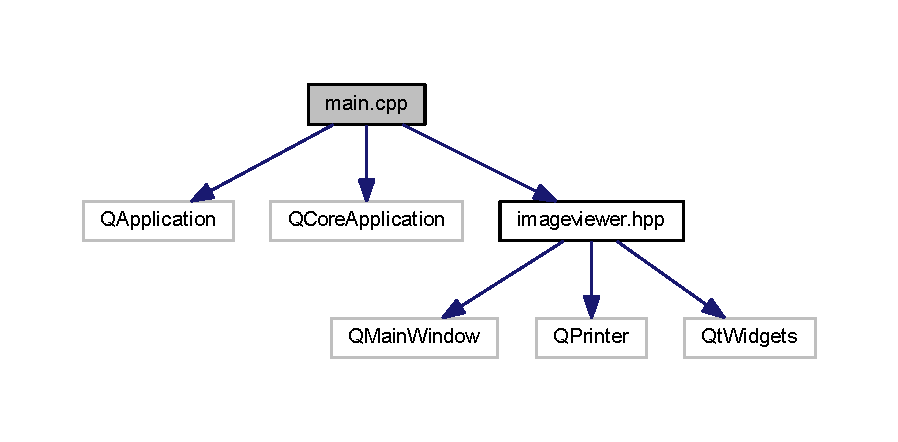
\includegraphics[width=350pt]{main_8cpp__incl}
\end{center}
\end{figure}
\subsection*{Functions}
\begin{DoxyCompactItemize}
\item 
\hypertarget{main_8cpp_a0ddf1224851353fc92bfbff6f499fa97}{int {\bfseries main} (int argc, char $\ast$argv\mbox{[}$\,$\mbox{]})}\label{main_8cpp_a0ddf1224851353fc92bfbff6f499fa97}

\end{DoxyCompactItemize}


\subsection{Detailed Description}
Ofeli. \begin{DoxyAuthor}{Author}
Fabien Bessy 
\end{DoxyAuthor}
\begin{DoxyVersion}{Version}
1.\-0.\-7 
\end{DoxyVersion}
\begin{DoxyDate}{Date}
August 2012 
\end{DoxyDate}


Definition in file \hyperlink{main_8cpp_source}{main.\-cpp}.


\chapter{Example Documentation}
\hypertarget{interface-example}{\section{interface}
}

\begin{DoxyCode}
\textcolor{comment}{// It interfaces the algorithm in order to display each iteration}

\textcolor{preprocessor}{#include "ac\_withoutedges.hpp"}
\textcolor{preprocessor}{#include "linked\_list.hpp"}
\textcolor{preprocessor}{#include <iostream>}

\textcolor{keywordtype}{int} offset \textcolor{comment}{// offset of the current pixel}
\textcolor{keywordtype}{unsigned} \textcolor{keywordtype}{char} I \textcolor{comment}{// intensity of the current pixel}

\textcolor{comment}{// Lout displayed in blue}
\textcolor{keywordtype}{unsigned} \textcolor{keywordtype}{char} Rout = 0;
\textcolor{keywordtype}{unsigned} \textcolor{keywordtype}{char} Gout = 0;
\textcolor{keywordtype}{unsigned} \textcolor{keywordtype}{char} Bout = 255;

\textcolor{comment}{// Lin displayed in red}
\textcolor{keywordtype}{unsigned} \textcolor{keywordtype}{char} Rin = 255;
\textcolor{keywordtype}{unsigned} \textcolor{keywordtype}{char} Gin = 0;
\textcolor{keywordtype}{unsigned} \textcolor{keywordtype}{char} Bin = 0;


\hyperlink{classofeli_1_1_a_cwithout_edges}{ofeli::ACwithoutEdges} ac(img1, img\_width1, img\_height1);


-----------------------------   Display the initial active contour   -----------------------------

\textcolor{keyword}{const} \hyperlink{classofeli_1_1list}{ofeli::list<int>}* Lout = &ac.get\_Lout();
\textcolor{keyword}{const} \hyperlink{classofeli_1_1list}{ofeli::list<int>}* Lin = &ac.get\_Lin();

\textcolor{comment}{// put the color of lists into the displayed buffer}
\textcolor{keywordflow}{for}( \hyperlink{classofeli_1_1list_1_1const__iterator}{ofeli::list<int>::const\_iterator} it = Lout->get\_begin(); !it.
      \hyperlink{classofeli_1_1list_1_1const__iterator_aa79779e28253e61c8d1816f577de4ffd}{end}(); ++it )
\{
    offset = *it*3;

    img\_displayed[offset] = Rout;
    img\_displayed[offset+1] = Gout;
    img\_displayed[offset+2] = Bout;
\}

\textcolor{keywordflow}{for}( \hyperlink{classofeli_1_1list_1_1const__iterator}{ofeli::list<int>::const\_iterator} it = Lin->get\_begin(); !it.end(); ++
      it )
\{
    offset = *it*3;

    img\_displayed[offset] = Rin;
    img\_displayed[offset+1] = Gin;
    img\_displayed[offset+2] = Bin;
\}

\textcolor{comment}{// paint event, refresh the widget witch display the buffer img\_displayed}
update();

\textcolor{comment}{// display the position of the active contour in the standard output}
std::cout << ac << std::endl;

--------------------------------------------------------------------------------------------------


\textcolor{comment}{// Loop for the evolution of the active contour}
\textcolor{keywordflow}{while}( !ac.get\_isStopped() )
\{
    \textcolor{comment}{// erase the previous lists Lout1 and Lin1 of the displayed buffer}
    \textcolor{keywordflow}{for}( \hyperlink{classofeli_1_1list_1_1const__iterator}{ofeli::list<int>::const\_iterator} it = Lout->get\_begin(); !it.
      \hyperlink{classofeli_1_1list_1_1const__iterator_aa79779e28253e61c8d1816f577de4ffd}{end}(); ++it )
    \{
        offset = *it;

        I = img1[offset];

        img\_displayed[3*offset] = I;
        img\_displayed[3*offset+1] = I;
        img\_displayed[3*offset+2] = I;
    \}

    \textcolor{keywordflow}{for}( \hyperlink{classofeli_1_1list_1_1const__iterator}{ofeli::list<int>::const\_iterator} it = Lin->get\_begin(); !it.end();
       ++it )
    \{
        offset = *it;

        I = img1[offset];

        img\_displayed[3*offset] = I;
        img\_displayed[3*offset+1] = I;
        img\_displayed[3*offset+2] = I;
    \}

    \textcolor{comment}{// to evolve the active contour of one iteration or one step}
    ++ac;

    \textcolor{comment}{// to get the temporary result}
    Lout = &ac.get\_Lout();
    Lin = &ac.get\_Lin();

    \textcolor{comment}{// put the color of lists into the displayed buffer}
    \textcolor{keywordflow}{for}( \hyperlink{classofeli_1_1list_1_1const__iterator}{ofeli::list<int>::const\_iterator} it = Lout->get\_begin(); !it.
      \hyperlink{classofeli_1_1list_1_1const__iterator_aa79779e28253e61c8d1816f577de4ffd}{end}(); ++it )

        offset = *it*3;

        img\_displayed[offset] = Rout;
        img\_displayed[offset+1] = Gout;
        img\_displayed[offset+2] = Bout;
    \}

    \textcolor{keywordflow}{for}( \hyperlink{classofeli_1_1list_1_1const__iterator}{ofeli::list<int>::const\_iterator} it = Lin->get\_begin(); !it.end();
       ++it )

        offset = *it*3;

        img\_displayed[offset] = Rin;
        img\_displayed[offset+1] = Gin;
        img\_displayed[offset+2] = Bin;
    \}

    \textcolor{comment}{// paint event, refresh the widget witch display the buffer img\_displayed}
    update();
\}
\end{DoxyCode}



\begin{DoxyCodeInclude}
\end{DoxyCodeInclude}
 
\hypertarget{linked_list-example}{\section{linked\-\_\-list}
}

\begin{DoxyCode}
\textcolor{comment}{// How to use the linked list ?}

\textcolor{preprocessor}{#include <iostream>}

\hyperlink{classofeli_1_1list}{ofeli::list<int>} list; \textcolor{comment}{// list is empty}
list.\hyperlink{classofeli_1_1list_a87b7f6a90670e08d99e23f3377b001f9}{push\_front}(99); \textcolor{comment}{// list = 99}
list.\hyperlink{classofeli_1_1list_a87b7f6a90670e08d99e23f3377b001f9}{push\_front}(99); \textcolor{comment}{// list = 99|99}
list.\hyperlink{classofeli_1_1list_a87b7f6a90670e08d99e23f3377b001f9}{push\_front}(2);  \textcolor{comment}{// list = 2|99|99}
list.\hyperlink{classofeli_1_1list_a87b7f6a90670e08d99e23f3377b001f9}{push\_front}(5);  \textcolor{comment}{// list = 5|2|99|99}
list.\hyperlink{classofeli_1_1list_a87b7f6a90670e08d99e23f3377b001f9}{push\_front}(99); \textcolor{comment}{// list = 99|5|2|99|99}
std::cout << list << std::endl;
\end{DoxyCode}
 
\begin{DoxyCode}
Standard output result :

     Linked list
---------------------
 Position | Value
---------------------
    1     |   99
    2     |   5
    3     |   2
    4     |   99
    5     |   99
---------------------
\end{DoxyCode}
 
\begin{DoxyCode}
list.\hyperlink{classofeli_1_1list_a87b7f6a90670e08d99e23f3377b001f9}{push\_front}(1);  \textcolor{comment}{// list = 1|99|5|2|99|99}
list.\hyperlink{classofeli_1_1list_a87b7f6a90670e08d99e23f3377b001f9}{push\_front}(99); \textcolor{comment}{// list = 99|1|99|5|2|99|99}
std::cout << list << std::endl;
\end{DoxyCode}
 
\begin{DoxyCode}
Standard output result :

     Linked list
---------------------
 Position | Value
---------------------
    1     |   99
    2     |   1
    3     |   99
    4     |   5
    5     |   2
    6     |   99
    7     |   99
---------------------
\end{DoxyCode}
 
\begin{DoxyCode}
\textcolor{comment}{// Removes all values of the list strictly greater than 50.}

\textcolor{comment}{// void begin() : the current position is the head of the list}
\textcolor{comment}{// bool end() : true if the current position is the tail of the list}

\textcolor{keywordflow}{for}( list.\hyperlink{classofeli_1_1list_a4f7f0567a64758636e3835ecea28a36f}{begin}(); !list.end(); )
\{
    \textcolor{keywordflow}{if}( list.get\_current() > 50 ) \textcolor{comment}{// if the value at the current position is greater than 50}
    \{
        list.\hyperlink{classofeli_1_1list_ae160d4ea7224becad437add3b1d594e4}{erase}(); \textcolor{comment}{// erase the value at the current position, the current position is the next
       element, now}
    \}
    \textcolor{keywordflow}{else}
    \{
        ++list; \textcolor{comment}{// similar to "++iterator;" for the STL list, moves to the next element in the list.}
    \}
\}
std::cout << list << std::endl;
\end{DoxyCode}
 
\begin{DoxyCode}
Standard output result :

     Linked list
---------------------
 Position | Value
---------------------
    1     |   1
    2     |   5
    3     |   2
---------------------
\end{DoxyCode}
 
\begin{DoxyCode}
list.\hyperlink{classofeli_1_1list_a1b4ab444619f6d412a461752ba019514}{clear}(); \textcolor{comment}{// list is empty}
list.\hyperlink{classofeli_1_1list_a87b7f6a90670e08d99e23f3377b001f9}{push\_front}(63);
std::cout << list << std::endl;
\end{DoxyCode}
 
\begin{DoxyCode}
Standard output result :

     Linked list
---------------------
 Position | Value
---------------------
    1     |   63
---------------------
\end{DoxyCode}
 
\begin{DoxyCode}
\textcolor{comment}{// If you want to read a list without modifying it. You should use const\_iterator.}
\textcolor{keywordflow}{for}( \hyperlink{classofeli_1_1list_1_1const__iterator}{ofeli::list<int>::const\_iterator} it = list.get\_begin(); !it.end(); ++
      it ) \textcolor{comment}{// scan through the list}
\{
    std::cout << \textcolor{stringliteral}{"value = "} << *it << std::endl;
\}
\end{DoxyCode}



\begin{DoxyCodeInclude}
\end{DoxyCodeInclude}
 
\addcontentsline{toc}{part}{Index}
\printindex
\end{document}
